\documentclass[oneside,11pt,dvipsnames]{book}
\setcounter{secnumdepth}{3}

\usepackage{xcolor}
\definecolor{myred}{RGB}{255,100,100}
\definecolor{yellowfill}{RGB}{255,245,200}
\definecolor{codegreen}{rgb}{0,0.6,0}
\definecolor{codegray}{rgb}{0.5,0.5,0.5}
\definecolor{codepurple}{rgb}{0.58,0,0.82}
\definecolor{backcolour}{rgb}{0.97,0.97,0.97}
\usepackage[utf8]{inputenc}
\usepackage[T1]{fontenc}
\usepackage[margin=1.5in]{geometry}
\usepackage{amsmath,amssymb,amsthm}
\usepackage{complexity}
\numberwithin{equation}{section}

\newtheorem{theorem}{Theorem}[section]
\newtheorem{lemma}{Lemma}[section]
\newtheorem{corollary}{Corollary}[section]

% Definitions and remarks usually use a different style:
\theoremstyle{definition}
\newtheorem{definition}{Definition}[section]
\newtheorem{example}{Example}[section]
\newtheorem{exercise}{Exercise}[section]

\theoremstyle{remark}
\newtheorem{remark}{Remark}


\usepackage{soul}
% \usepackage[small,compact]{titlesec} %very powerful
\usepackage[most]{tcolorbox}
% \setsecnumdepth{subsection}
% \setcounter{tocdepth}{3}
\usepackage{multirow,multicol}
\usepackage{enumitem}
\usepackage{epigraph}
\usepackage{cite}
\usepackage{caption}
\captionsetup{font=small}
\usepackage{graphicx}
\usepackage{pdfpages}
\usepackage{wrapfig}
\usepackage{subcaption}
\setlength\intextsep{0pt} % remove extra space above and below in-line float
\usepackage{hyperref}
\hypersetup{
  colorlinks,
  citecolor=black,
  filecolor=black,
  linkcolor=blue,
  urlcolor=blue,
}
\usepackage{cleveref}
\usepackage{booktabs}
\usepackage{tikz}
\usetikzlibrary{calc,positioning}
\usepackage{pgfplots}
\pgfplotsset{compat=1.18}



\usepackage{anyfontsize}
\usepackage{sectsty}

\usepackage[makeroom]{cancel}

\usepackage[linesnumbered,ruled,vlined]{algorithm2e}

\SetKwFor{Parfor}{parfor}{do}{endparfor}

\SetKwInOut{Input}{input}
\SetKwInOut{Output}{output}

\SetKw{Break}{break}
\SetKw{Continue}{continue}
\SetKw{In}{in}
\SetKwData{certified}{certified}
\SetKwData{prooftree}{proof}
\SetKwData{uncertified}{uncertified}
\SetKwData{model}{model}
\SetKwData{leaf}{node}
\SetKwData{mynull}{null}
\SetKwData{layer}{layer}
\SetKwData{layer}{layer}
\SetKwData{layerbounds}{layer\_bounds}
\DontPrintSemicolon


\SetAlgoCaptionSeparator{.}
\SetAlCapFnt{\footnotesize\rm}
\SetAlCapNameFnt{\footnotesize\rm}

\newcommand{\functiontextformat}[1]{\textrm{\texttt{#1}}}


\newtoggle{usecomment}
\settoggle{usecomment}{true}

\newcommand{\tcomment}[1]{\iftoggle{usecomment}{#1}{}}
\newcommand{\tvn}[1]{\iftoggle{usecomment}{{\color{red}{[TVN]: #1}}}{}}

\newcommand{\mbd}[1]{\iftoggle{usecomment}{{\color{magenta}{[MBD]: #1}}}{}}
\newcommand{\hd}[1]{\iftoggle{usecomment}{{\color{blue}{[HD]: #1}}}{}}
\newcommand{\hai}[1]{\iftoggle{usecomment}{{\color{blue}{[HD]: #1}}}{}}

\newcommand{\mynew}[1]{\iftoggle{usecomment}{{\color{red}{[NEW]: #1}}}{}}

%\newcommand{\ignore}[1]{}



\newtcolorbox{mybox}{
  enhanced,
  boxrule=0pt,frame hidden,
  borderline west={2pt}{0pt}{green!75!black},
  colback=green!10!white,
  sharp corners
}

\newenvironment{commentbox}[1][]{
  \small
  \begin{mybox}
    {\small \textbf{#1}}
  }{
  \end{mybox}
}

\newtcolorbox{mydomesticbox}{
  enhanced,
  boxrule=0pt,frame hidden,
  borderline west={2pt}{0pt}{red!75!black},
  colback=blue!10!white,
  sharp corners
}

\newenvironment{domesticbox}[1][]{
  \small
  \begin{mydomesticbox}
    {\small \textbf{#1}}
  }{
  \end{mydomesticbox}
}

\newcommand{\ignore}[1]{}

% for captions
%\def\Section{\S}
%\newcommand{\Section}{\textsection\@gobble}
\renewcommand{\figurename}{Fig.}
\renewcommand{\tablename}{Tab.}
\renewcommand{\algorithmcfname}{Alg.}

\makeatletter
% for cross references
% \renewcommand{\algorithmcflinename}{L.}
\renewcommand{\algorithmautorefname}{Alg.}
\renewcommand{\figureautorefname}{Fig.}
\renewcommand{\tableautorefname}{Tab.}
\renewcommand{\equationautorefname}{Eq.}
%\renewcommand{\exampleautorefname}{Ex.}
\renewcommand{\chapterautorefname}{\textsection\@gobble}
\renewcommand{\sectionautorefname}{\textsection\@gobble}
\renewcommand{\subsectionautorefname}{\textsection\@gobble}
\renewcommand{\subsubsectionautorefname}{\textsection\@gobble}
\renewcommand{\appendixautorefname}{\textsection\@gobble}

% \renewcommand{\chapterautorefname}{\S\@gobble}
% \renewcommand{\sectionautorefname}{\S\@gobble}
% \renewcommand{\subsectionautorefname}{\S\@gobble}
% \renewcommand{\appendixautorefname}{\S\@gobble}

\makeatother
\newcommand{\proofgen}{\texttt{BaB$_{\text{ProofGen}}$}}
\newcommand{\prooflang}{\texttt{BaB$_{\text{ProofLang}}$}}
\newcommand{\proofcheck}{\texttt{BaB$_{\text{ProofCheck}}$}}

\newcommand{\veristable}{\texttt{VeriStable}}
\newcommand{\crown}{\texttt{$\alpha\beta$-CROWN}}
\newcommand{\nnenum}{\texttt{nnenum}}
\newcommand{\marabou}{\texttt{Marabou}}
\newcommand{\eran}{\texttt{ERAN}}
\newcommand{\reluplex}{\texttt{Reluplex}}
\newcommand{\reluval}{\texttt{Reluval}}
\newcommand{\neurify}{\texttt{Neurify}}
\newcommand{\nnv}{\texttt{NNV}}
\newcommand{\ovalnnv}{\texttt{OVAL}}
\newcommand{\dnnv}{\texttt{DNNV}}
\newcommand{\verinet}{\texttt{VeriNet}}
\newcommand{\mnbab}{\texttt{MN-BaB}}
% \newcommand{\vnncomp}{VNN-COMP'23}
\newcommand{\planet}{\texttt{Planet}}
\newcommand{\bab}{\texttt{BaB$_{\text{NV}}$}}
\newcommand{\neuralsat}{\texttt{NeuralSAT}}
\newcommand{\tool}{\texttt{NeuralSAT}}
\newcommand{\mipverify}{\texttt{MIPVerify}}
\newcommand{\crowndefault}{\texttt{$\alpha\beta$-CROWN} (default)}

\newcommand{\relu}[1]{\mathrm{ReLU}\left(#1\right)}
\newcommand{\sigmoid}[1]{\mathrm{sigmoid}\left(#1\right)}
\newcommand{\mytanh}[1]{\mathrm{tanh}\left(#1\right)}
\newcommand{\softmax}[1]{\mathrm{softmax}\left(#1\right)}

\newcommand{\sat}{\texttt{sat}}
\newcommand{\unsat}{\texttt{unsat}}


\lstdefinelanguage{SMTLIB}{
    morekeywords={assert, declare-const, declare-pwl, or, and, },
    alsoletter={-},
    morecomment=[l];,
    morestring=[b]",
    morekeywords=[2]{Real, Int, ReLU},
    keywordstyle=[2]\color{codepurple},
}

\lstdefinestyle{SMTLIB-style}{
    backgroundcolor=\color{backcolour},   
    commentstyle=\color{codegreen},
    keywordstyle=\color{blue},
    numberstyle=\tiny\color{black},
    stringstyle=\color{codepurple},
    basicstyle=\ttfamily\footnotesize,
    breakatwhitespace=false, 
    breaklines=true, 
    captionpos=b, 
    keepspaces=true, 
    numbers=left, 
    numbersep=5pt, 
    showspaces=false, 
    showstringspaces=false,
    showtabs=false, 
    tabsize=2,
}

\lstset{
    language=SMTLIB,
    style=SMTLIB-style
}


\begin{document}

\pagestyle{empty}
\begin{tikzpicture}[overlay,remember picture]

    % Background color
    \fill[
    black!2]
    (current page.south west) rectangle (current page.north east);
    
    % Rectangles
    \shade[
    left color=Dandelion, 
    right color=Dandelion!40,
    transform canvas ={rotate around ={45:($(current page.north west)+(0,-6)$)}}] 
    ($(current page.north west)+(0,-6)$) rectangle ++(9,1.5);
    
    \shade[
    left color=lightgray,
    right color=lightgray!50,
    rounded corners=0.75cm,
    transform canvas ={rotate around ={45:($(current page.north west)+(.5,-10)$)}}]
    ($(current page.north west)+(0.5,-10)$) rectangle ++(15,1.5);
    
    \shade[
    left color=lightgray,
    rounded corners=0.3cm,
    transform canvas ={rotate around ={45:($(current page.north west)+(.5,-10)$)}}] ($(current page.north west)+(1.5,-9.55)$) rectangle ++(7,.6);
    
    \shade[
    left color=orange!80,
    right color=orange!60,
    rounded corners=0.4cm,
    transform canvas ={rotate around ={45:($(current page.north)+(-1.5,-3)$)}}]
    ($(current page.north)+(-1.5,-3)$) rectangle ++(9,0.8);
    
    \shade[
    left color=red!80,
    right color=red!80,
    rounded corners=0.9cm,
    transform canvas ={rotate around ={45:($(current page.north)+(-3,-8)$)}}] ($(current page.north)+(-3,-8)$) rectangle ++(15,1.8);
    
    \shade[
    left color=orange,
    right color=Dandelion,
    rounded corners=0.9cm,
    transform canvas ={rotate around ={45:($(current page.north west)+(4,-15.5)$)}}]
    ($(current page.north west)+(4,-15.5)$) rectangle ++(30,1.8);
    
    \shade[
    left color=RoyalBlue,
    right color=Emerald,
    rounded corners=0.75cm,
    transform canvas ={rotate around ={45:($(current page.north west)+(13,-10)$)}}]
    ($(current page.north west)+(13,-10)$) rectangle ++(15,1.5);
    
    \shade[
    left color=ForestGreen,
    rounded corners=0.3cm,
    transform canvas ={rotate around ={45:($(current page.north west)+(18,-8)$)}}]
    ($(current page.north west)+(18,-8)$) rectangle ++(15,0.6);
    
    \shade[
    left color=ForestGreen,
    rounded corners=0.4cm,
    transform canvas ={rotate around ={45:($(current page.north west)+(19,-5.65)$)}}]
    ($(current page.north west)+(19,-5.65)$) rectangle ++(15,0.8);
    
    \shade[
    left color=OrangeRed,
    right color=red!80,
    rounded corners=0.6cm,
    transform canvas ={rotate around ={45:($(current page.north west)+(20,-9)$)}}] 
    ($(current page.north west)+(20,-9)$) rectangle ++(14,1.2);
    
 
    
    % Title
    \node[align=center] at ($(current page.center)+(0,-5)$) 
    {
        {\fontsize{24}{24} \selectfont {{Engineering A Verifier}}} \\[0.15in]
        {\fontsize{24}{24} \selectfont {{for Deep Neural Networks}}} \\[1in]    
        %{\fontsize{18}{18} \selectfont {{A Handbook for International Students}}} \\[1.in]

        {\fontsize{14}{19.2} \selectfont \textcolor{ForestGreen}{ \bf ThanhVu Nguyen}}\\[0.1in]
        {\fontsize{14}{19.2} \selectfont \textcolor{ForestGreen}{ \bf Hai Duong}}\\[0.1in]
    \today{} (latest version available on  \href{https://github.com/nguyenthanhvuh/book_nnv}{Github})
    };
    \end{tikzpicture}

    
\chapter*{Preface}

% \begin{mybox}
% This document will be updated regularly to reflect the latest information and updates in the admission process. Its latest version is available at

% \begin{center}
%   \href{https://nguyenthanhvuh.github.io/phd-cs-us/demystify.pdf}{nguyenthanhvuh.github.io/phd-cs-us/demystify.pdf},
% \end{center}

% \noindent and its \LaTeX{} source is also on \href{https://github.com/nguyenthanhvuh/phd-cs-us}{GitHub}. If you have questions or comments, feel free to create new \href{https://github.com/nguyenthanhvuh/phd-cs-us/issues}{GitHub issues} or \href{https://github.com/nguyenthanhvuh/phd-cs-us/discussions}{discussions}.

%\end{mybox}

\newpage
\tableofcontents

\part{Basics of Neural Networks and Verification}
\chapter{Neural Networks}\label{sec:basic}

\section{Basics of Neural Networks}
A \emph{neural network} (\textbf{NN})~\cite{Goodfellow-et-al-2016} consists of an input layer, multiple hidden layers, and an output layer. Each layer has a number of neurons, each connected to neurons in the next layer through a predefined set of weights (derived by training the network with data). A \emph{Deep Neural Network} (\textbf{DNN}) is an NN with two or more hidden layers. 

%A deep neural network consists of three types of layers: an input layer, multiple hidden layers, and an output layer. Each layer consists of a number of neurons, each connected to neurons from another layers through a predefined set of weights (derived by training the network with data). A network is called a \emph{fully connected feed-forward} neural network (FNN) if it connects every neuron in a layer (i.e., all weights are non-zero) to a neuron in the next layer.

The output of an NN is obtained by iteratively computing  the  values  of  neurons  in  each  layer.
The value of a neuron in the input layer is the input data. The value of a neuron in the hidden layers is computed by applying an \emph{affine transformation} (\autoref{sec:affine}) to values of neurons in the previous layers, then followed by an \emph{activation function} (\autoref{sec:activation}) such as ReLU and Sigmoid. The value of a neuron in the output layer is computed similarly but may skip the activation function.

\paragraph{NN as a Function} We can view an NN as a function that maps input vectors to output vectors: 
\begin{equation}
f: \mathbb{R}^{n} \to \mathbb{R}^{m}
\end{equation}
where \(n\) is the number of input neurons and \(m\) is the number of output neurons. The neurons in the input layer are the inputs to the function, and the neurons in the output layer are the outputs of the function. The neurons in the hidden layers are also functions that transform the inputs from the previous layer to produce outputs for the next layer.

%Fig.~\ref{fig:dnn}b shows the same network but with each hidden neuron $x$ split into two neurons $x'$ and $x''$ representing the result of affine transformation on $x$ and ReLU activation on $x'$, respectively, e.g.,  $x_3'=-x_1-0.5x_2-1.0$ and  $x_3'' = ReLU(x_3')$. This ReLU-slitting representation is adopted by \tool{} and other DNN analyses (e.g., ~\cite{katz2017reluplex,wang2018efficient,henriksen2020efficient}) 
% including Reluplex~\cite{katz2017reluplex}, Neurify~\cite{wang2018efficient}, and VeriNet~\cite{henriksen2020efficient},
%because it does not change the semantics or complexity of the problem and is easier to reason about as we will show in \S\ref{sec:overview}.

% \section{The Basics}\label{sec:nn-basics}




% \paragraph{Graph Structure} A neural network (NN) can be viewed as a special kind of \emph{directed acyclic graph (DAG)} where each node represents a computation unit that receives inputs from its parent nodes and produces outputs for its child nodes. %Typically, neural networks are organized into layers, although more complex architectures may deviate from strict layer-wise organization (e.g., residual networks, attention models). 
% Overall, the NN defines a composite function \( f \) mapping vectors of real numbers to vectors of real numbers:
% \begin{align}
% f: \mathbb{R}^{n} \to \mathbb{R}^{m}
% \end{align}
% where $n, m$ are the dimensions of the input and output vectors, respectively.


% \begin{figure}[htp]
%     \centering
%     \begin{tikzpicture}[
%         every node/.style={draw, circle, minimum size=8mm, thick, font=\large, inner sep=0pt},
%         xnode/.style={draw=red!60!black, fill=red!15},
%         vnode/.style={draw=cyan!60!black, fill=cyan!40},
%         ynode/.style={draw=green!60!black, fill=green!15}
%       ]
%       % Nodes
%       \node[xnode]   (x) at (0,0)    {$x$};
%       \node[vnode]   (v) at (2.5,0)  {$v$};
%       \node[ynode]   (y) at (5,0)    {$y$};
%       % Arrows
%       \draw[->, thick] (x) -- (v);
%       \draw[->, thick] (v) -- (y);
%     \end{tikzpicture}
%     \caption{A simple neural network with 3 nodes.}
%     \label{fig:snn}
% \end{figure}

% \begin{example}\label{ex:nn3}
% \Cref{fig:snn} illustrates a simple neural network with three nodes:

% \begin{enumerate}
%     \item The \textbf{input node} \(x\) (red) simply receives the external input value \(r \in \mathbb{R}\) and passes it forward without any modification.

%     \item The \textbf{hidden node} \(v\) (cyan) applies a linear transformation:
%     \[
%     v = 2r + 1.
%     \]

%     \item The \textbf{output node} \(y\) (green) applies a non-linear activation function, in this case, the ReLU function:
%     \[
%     y = \relu{v} = \max(0, v).
%     \]
% \end{enumerate}

% Thus, the network defines the function \(f: \mathbb{R} \to \mathbb{R}\) given by:
% \begin{align}
% f(r) = \relu{2r + 1}.
% \end{align}
% \end{example}

\newcommand{\mydnn}{
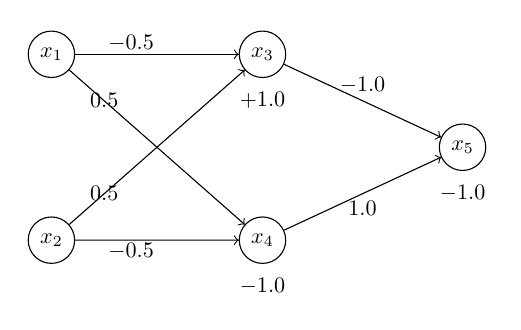
\begin{tikzpicture}[scale=0.8, transform shape]
    % Input nodes
    \node[circle, draw] (x1) {$x_1$};
    \node[circle, draw, below=2.2cm of x1]  (x2) {$x_2$};

    % Hidden layer
    \node[circle, draw, right=2.6cm of x1] (x3) {$x_3$};
    \node[circle, draw, right=2.6cm of x2] (x4) {$x_4$};

    % Output layer node (centered horizontally)
    \coordinate (mid) at ($(x3)!0.5!(x4)$);
    \node[circle, draw, right=2.8cm of mid] (x5) {$x_5$};

    % Connections with weights
    \draw[->] (x1) -- node[above left=-3pt] {$-0.5$} (x3);
    \draw[->] (x1) -- node[pos=0.2] {$0.5$} (x4);
    \draw[->] (x2) -- node[pos=0.2] {$0.5$} (x3);
    \draw[->] (x2) -- node[below left=-3pt] {$-0.5$} (x4);
    \draw[->] (x3) -- node[above] {$-1.0$} (x5);
    \draw[->] (x4) -- node[below] {$1.0$} (x5);

    % Output weights under x3, x4, x5 (biases)
    \node[below=0.1cm of x3] {$+1.0$};
    \node[below=0.1cm of x4] {$-1.0$};
    \node[below=0.1cm of x5] {$-1.0$};
\end{tikzpicture}
}

\begin{figure}
    \centering
    \mydnn
    \caption{\label{fig:dnn}A simple DNN with two inputs $x_1,x_2$, two hidden neurons $x_3,x_4$, and one output neuron $x_5$.}
\end{figure}

\begin{example}\label{ex:dnn}
\Cref{fig:dnn} shows an NN with two inputs $x_1, x_2 \in \mathbb{R}$, two hidden neurons \(x_3, x_4\) in one hidden layer, and one output neuron \(x_5\). The connections between the neurons are weighted edges, and the biases are shown below each neuron.


\begin{itemize}
    \item The hidden neurons compute:
    \[
    x_3 = \relu{-0.5 x_1 + 0.5 x_2 + 1.0},\quad x_4 = \relu{1.0 x_1 + 1.0 x_2 - 1.0},
    \]
    where $\relu{x} = \max(x, 0)$ is the ReLU activation function.
    \item The output neuron computes:
    \[
    x_5 = -1.0 \cdot x_3 + 1.0 \cdot x_4 - 1.0.
    \]
\end{itemize}

Thus, this NN computes a function \(f: \mathbb{R}^2 \to \mathbb{R}\) where:
\[
f(x_1, x_2) = -\relu{-0.5 x_1 + 0.5 x_2 + 1.0} + \relu{1.0 x_1 + 1.0 x_2 - 1.0} - 1.0.
\]
\end{example}


\section{Affine Transformation}\label{sec:affine}

The affine transformation (AF) of a neuron consists of a \emph{linear combination}---i.e., a weighted sum---of its inputs, followed by the addition of a bias term. More specifically, for a neuron with weights \(w_1, \dots, w_n\), bias \(b\), and inputs \(v_1, \dots, v_n\) from the previous layer, the affine transformation computes:

\begin{equation}\label{eq:affine}   
    f(v_1, v_2, \dots,v_n) = \sum_{i=1}^{n} w_i v_i + b.
\end{equation}


\begin{example}
In \autoref{fig:dnn}, neuron \(x_3\) receives inputs \(x_1\) and \(x_2\) with weights \(-0.5\), \(0.5\), and bias \(1.0\), so its affine transformation is $x_3 = -0.5 x_1 + 0.5 x_2 + 1.0$.
\end{example}


\section{Activation Functions}\label{sec:activation}
Popular activation functions used in NNs include ReLU, Sigmoid, Tanh, and Softmax. All of these are non-linear\footnote{Non-linear means that the output of the function is not a linear combination of its inputs.} functions that introduce non-linearity to the network, allowing it to learn complex patterns in the data.

\autoref{tab:activation} summarizes the most common activation functions used in NNs, their equations, output ranges, and key uses.

\begin{table}
  \centering
  \caption{Summary of Common Neural Network Activation Functions}\label{tab:activation}
  \small
  \begin{tabular}{llll}
    \toprule
    \textbf{Name} & \textbf{Equation} & \textbf{Output Range} & \textbf{Key Use} \\
    \midrule
    ReLU      & $ \max(0, x) $                   & $[0, \infty)$   & Hidden layers, fast train \\    
    Sigmoid   & $ \frac{1}{1 + e^{-x}} $         & $(0, 1)$        & Binary classification \\
    Tanh      & $ \tanh(x) $                     & $(-1, 1)$       & Hidden layers, zero-centered \\
    Softmax   & $ \frac{e^{x_i}}{\sum_j e^{x_j}} $& $(0, 1), \sum_i=1 $ & Multi-class output \\    
    % Leaky ReLU& $ \begin{cases} x & x>0 \\ \alpha x & x\leq 0 \end{cases} $ & $(-\infty, \infty)$ & Prevent dead neurons \\
    % Swish     & $ x \cdot \sigmoid{x} $  & $(-\infty, \infty)$ & Deep networks \\
    % ELU       & $ \begin{cases} x & x>0 \\ \alpha(e^{x}-1) & x\leq 0 \end{cases} $ & $(-\alpha, \infty)$ & Advanced networks \\
    \bottomrule
  \end{tabular}
\end{table}


\subsection{ReLU (Rectified Linear Unit)}\label{sec:relu}

ReLU is a widely used activation function in NNs. It is defined as:

\[
\relu{x} = \max(0, x) = 
\begin{cases}
0 & \text{if } x \leq 0 \\
x & \text{if } x > 0
\end{cases}
\]

ReLU is \textbf{piecewise linear} because it consists of two linear segments as shown as in \autoref{fig:relu}: (i) a constant function ($0$) when $x \leq 0$, (ii) and (ii) a linear function ($x$) when $x > 0$.
A ReLU activated neuron is said to be \emph{active} if its input is greater than zero and \emph{inactive} otherwise.


\begin{figure}[h]
    \centering
    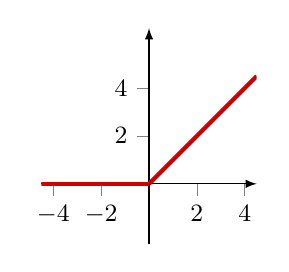
\begin{tikzpicture}
        \begin{axis}[
            width=1.7in, height=1.7in,
            axis x line=middle, axis y line=middle,
            xlabel={}, ylabel={},
            axis equal,
            xtick={-4, -2, 0, 2, 4},
            ytick={0, 2, 4},
            xmin=-4.5, xmax=4.5, ymin=-0.5, ymax=4.5,
            enlargelimits=false,
            samples=2,
            domain=-4.5:4.5,
            axis line style={-latex},
            tick label style={font=\small},
            % yticklabel style={font=\small},
            % xticklabel style={font=\small},
            tick align=outside,
            minor tick num=0,
        ]
        % ReLU curve: flat at zero, then linear
        \addplot[line width=1.5pt, red!80!black, samples=2, domain=-4.5:0] {0};
        \addplot[line width=1.5pt, red!80!black, domain=0:4.5] {x};
      \end{axis}
    \end{tikzpicture}
    \caption{ReLU (Rectified Linear Unit) function.}\label{fig:relu}
\end{figure}

\begin{example}
$\relu{-1.2} = 0$ (inactive), $\relu{0} = 0$ (inactive), and $\relu{2.8} = 2.8$ (active).
\end{example}


However, despite being piecewise linear, ReLU is \textbf{nonlinear} because it does not satisfy the two core properties of a linear function

    \begin{itemize}
        \item \textit{Additivity:} $\text{ReLU}(x + y) \ne \text{ReLU}(x) + \text{ReLU}(y)$ in general,
        \item \textit{Homogeneity:} $\text{ReLU}(\alpha x) \ne \alpha \cdot \text{ReLU}(x)$ when $\alpha < 0$.
    \end{itemize}

In simpler terms, ReLU is nonlinear because it does not form a straight line.  It has a \textbf{kink} (a sharp bend) at $x = 0$, where the slope changes abruptly from $0$ to $1$. This discontinuity in the derivative prevents the function from being globally linear.


This non-linearity makes DNN verification difficult. In fact, verification NNS with ReLU is $\mathsf{NP}$-complete as shown in~\autoref{sec:complexity}. We will use ReLU throughout this book as the default activation function for hidden neurons in an NN.

\subsection{Sigmoid}\label{sec:sigmoid}



\begin{figure}[ht]
    \centering
    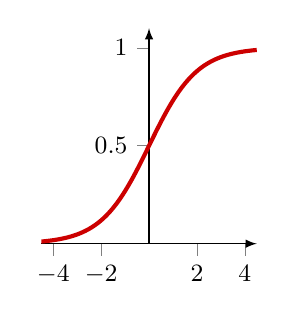
\begin{tikzpicture}
        \begin{axis}[
            width=1.7in, height=1.7in,
            axis x line=middle, axis y line=middle,
            xlabel={}, ylabel={},
            xtick={-4, -2, 0, 2, 4},
            ytick={0, 0.5, 1},
            xmin=-4.5, xmax=4.5, ymin=0, ymax=1.1,
            enlargelimits=false,
            samples=300,
            domain=-4.5:4.5,
            axis line style={-latex},
            tick label style={font=\small},
            % yticklabel style={font=\small},
            % xticklabel style={font=\small},
            tick align=outside,
            minor tick num=0,
        ]
        \addplot[line width=1.5pt, red!80!black, samples=300, domain=-4.5:4.5] {1/(1 + exp(-x))};
      \end{axis}
    \end{tikzpicture}
    \caption{Sigmoid function.}\label{fig:sigmoid}
\end{figure}

Sigmoid, shown in~\autoref{fig:sigmoid}, is a smooth---i.e., continuous and differentiable---non-linear activation function that maps any real value to the range (0,1).
It is continuous, meaning that small changes in the input will result in small changes in the output, and differentiable, meaning that it has a well-defined derivative at every point. Sigmoid is often used in the output layer of a binary classification problem.

    \begin{align}
        \sigmoid{x} = \frac{1}{1+e^{-x}}
    \end{align}

\begin{example}
$\sigmoid{-1.2} \approx 0.23$, $\sigmoid{0} = 0.5$, and $\sigmoid{2.8} \approx 0.94$. This means that the sigmoid function maps -1.2 to a value close to 0, 0 to 0.5, and 2.8 to a value close to 1.
\end{example}

\subsection{Hyperbolic Tangent (Tanh)}\label{sec:tanh}

Tanh, shown in~\autoref{fig:tanh}, is similar to sigmoid (\autoref{sec:sigmoid})  but maps any real value to the range (-1,1). It is often used in the output layer of a multi-class classification problem.

\begin{figure}[htp]
    \centering
    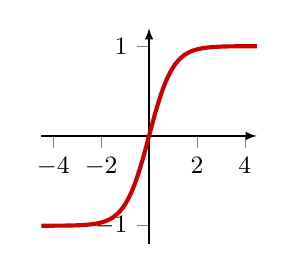
\begin{tikzpicture}
        \begin{axis}[
            width=1.7in, height=1.7in,
            axis x line=middle, axis y line=middle,
            xlabel={}, ylabel={},
            xtick={-4, -2, 0, 2, 4},
            ytick={-1, 0, 1},
            xmin=-4.5, xmax=4.5, ymin=-1.2, ymax=1.2,
            enlargelimits=false,
            samples=300,
            domain=-4.5:4.5,
            axis line style={-latex},
            tick label style={font=\small},
            tick align=outside,
            minor tick num=0,
        ]
        % tanh curve
        \addplot[line width=1.5pt, red!80!black, samples=300, domain=-4.5:4.5] {tanh(x)};
        % 0.0 label at origin, slightly offset
      \end{axis}
    \end{tikzpicture}
    \caption{tanh (hyperbolic tangent) activation function.}\label{fig:tanh}
\end{figure}

\begin{align}
\tanh(x) = \frac{e^x-e^{-x}}{e^x+e^{-x}}
\end{align}

\begin{example}
$\tanh(-1.2) \approx -0.83$, $\tanh(0) = 0$, and $\tanh(2.8) \approx 0.99$. This means that the tanh function maps -1.2 to a value close to -1, 0 to 0, and 2.8 to a value close to 1.
\end{example}

\subsection{Softmax}\label{sec:softmax}


\begin{figure}[htp]
    \centering
    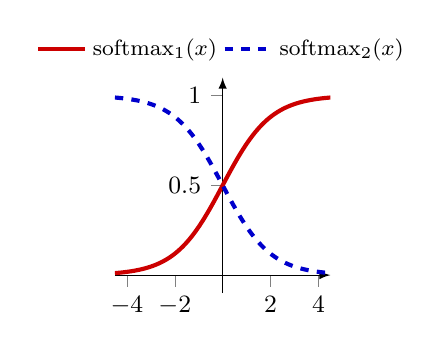
\begin{tikzpicture}
        \begin{axis}[
            width=1.7in, height=1.7in,
            axis x line=middle, axis y line=middle,
            % axis equal,
            xlabel={}, ylabel={},
            xtick={-4, -2, 0, 2, 4},
            ytick={0, 0.5, 1},
            xmin=-4.5, xmax=4.5, ymin=-0.1, ymax=1.1,
            enlargelimits=false,
            samples=200,
            domain=-4.5:4.5,
            axis line style={-latex},
            tick label style={font=\small},
            tick align=outside,
            minor tick num=0,
            legend style={at={(0.5,1.03)},anchor=south,legend columns=2,draw=none, font=\footnotesize},
        ]
        % softmax_1 curve
        \addplot[line width=1.5pt, red!80!black, domain=-4.5:4.5] {exp(x)/(exp(x)+1)};
        % softmax_2 curve
        \addplot[line width=1.5pt, blue!80!black, domain=-4.5:4.5, dashed] {1/(exp(x)+1)};
        % Add legends
        \addlegendentry{$\mathrm{softmax}_1(x)$}
        \addlegendentry{$\mathrm{softmax}_2(x)$}
      \end{axis}
    \end{tikzpicture}
    \caption{Softmax function for 2 classes.}\label{fig:softmax}
\end{figure}


Softmax, shown in~\autoref{fig:softmax}, is a generalization of sigmoid (\autoref{sec:sigmoid}) that maps any real value to the range (0,1) and ensures that the sum of the output values is 1. It is often used in the output layer of a multi-class classification problem.
\begin{align}
\softmax{x}_i = \frac{e^{x_i}}{\sum_{j=1}^{n}e^{x_j}}
\end{align}

\begin{example}
For a vector $x = [2, 1, 0]$, softmax computes: 

{\small
\begin{align*}
\softmax{x} &= \left[\frac{e^2}{e^2+e^1+e^0}, \frac{e^1}{e^2+e^1+e^0}, \frac{e^0}{e^2+e^1+e^0}\right] \\
&= \left[\frac{7.389}{7.389+2.718+1}, \frac{2.718}{7.389+2.718+1}, \frac{1}{7.389+2.718+1}\right] \\
&\approx [0.71, 0.24, 0.05]
\end{align*}
}

This means that softmax maps the input vector $x$ to a probability distribution over the three classes, where the first class has a probability of 0.71, the second class has a probability of 0.24, and the third class has a probability of 0.05.
\end{example}


\section{Neural Network Architectures and Layers}

NNs vary in architecture depending on how information flows through them and how computations are structured. Most common models are variations of the \emph{feedforward network}, with additional structures or constraints layered on top.  \autoref{tab:nn-types} summarizes several common NN architectures and their typical application domains.

\begin{table}[ht]
\caption{Popular NN Architectures and Applications}\label{tab:nn-types}
\centering
\small
\begin{tabular}{llp{8cm}@{}}
\toprule
\textbf{Name} & \textbf{Acronym} & \textbf{Typical Applications} \\
\midrule
Feedforward NN & FNN / MLP & General function approximation, tabular data \\
Convolutional NN & CNN & Image processing, video analysis \\
Residual NN & ResNet & Deep image recognition, medical imaging \\
Recurrent NN & RNN & Sequence modeling, NLP, time series \\
Transformer & -- & NLP, summarization, code generation, vision \\
Graph NN & GNN & Graph-structured data, molecule modeling, recommendation \\
\bottomrule
\end{tabular}
\end{table}




\subsection{Feedforward Neural Networks (FNNs)}\label{sec:ffn}

In an FNN, information flows in one direction: from the input layer, through one or more hidden layers, and finally to the output layer. There are no loops or cycles in the computation graph. 

Widely used feedforward architectures include fully connected, convolutional, and residual networks. Each architecture has its own strengths and is suited for different types of tasks.

\paragraph{Fully Connected NNs}

In fully connected NNs, each neuron in a layer is connected to every neuron in the next layer. Thus, every neuron in the input layer is connected to every neuron in the first hidden layer, every neuron in the first hidden layer is connected to every neuron in the second hidden layer, and so on, until the output layer. Fully connected NNs, sometimes called \emph{dense networks}, are the most basic type of FNNs and are commonly used for tasks like classification. 

\begin{example}
\autoref{fig:dnn} earlier showed a fully connected network with two inputs and one hidden layer with two neurons, and one output neuron. \autoref{fig:ffn} below shows a fully connected network with four inputs, two hidden layers with five neurons each, and three output neurons (weights and biases not shown for simplicity).

\begin{figure}[htp]
    \centering
    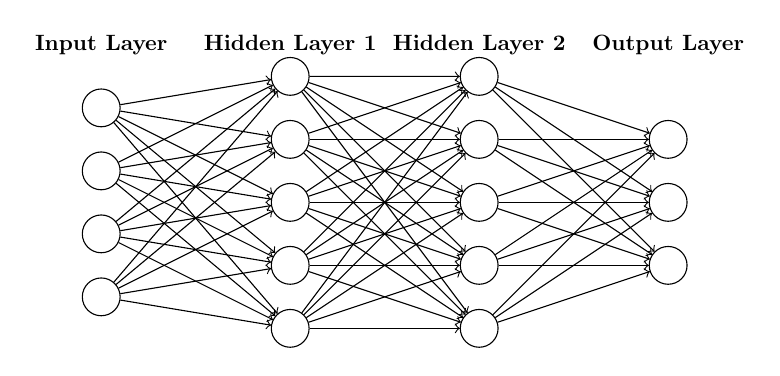
\begin{tikzpicture}[scale=0.8, transform shape]
        % Input Layer
        \node at (0,4) {\textbf{Input Layer}};
        \foreach \x in {1,2,3,4} {
            \node[circle, draw=black, fill=white, minimum size=0.6cm] (I\x) at (0,4-\x) {};
        }

        % Hidden Layer 1
        \node at (3,4) {\textbf{Hidden Layer 1}};
        \foreach \x in {1,2,3,4,5} {
            \node[circle, draw=black, fill=white, minimum size=0.6cm] (H1\x) at (3,4.5-\x) {};
        }

        % Hidden Layer 2
        \node at (6,4) {\textbf{Hidden Layer 2}};
        \foreach \x in {1,2,3,4,5} {
            \node[circle, draw=black, fill=white, minimum size=0.6cm] (H2\x) at (6,4.5-\x) {};
        }

        % Output Layer
        \node at (9,4) {\textbf{Output Layer}};
        \foreach \x in {1,2,3} {
            \node[circle, draw=black, fill=white, minimum size=0.6cm] (O\x) at (9,3.5-\x) {};
        }

        % Connections
        \foreach \i in {1,2,3,4}
            \foreach \j in {1,2,3,4,5}
                \draw[->] (I\i) -- (H1\j);

        \foreach \i in {1,2,3,4,5}
            \foreach \j in {1,2,3,4,5}
                \draw[->] (H1\i) -- (H2\j);

        \foreach \i in {1,2,3,4,5}
            \foreach \j in {1,2,3}
                \draw[->] (H2\i) -- (O\j);
    \end{tikzpicture}
    \caption{A fully connected NN with two hidden layers.}
    \label{fig:ffn}
\end{figure}
\end{example}


\paragraph{Convolutional NNs (CNNs)} CNNs replace fully connected layers with \emph{convolutional layers}, which apply local filters across the input space. In CNNs, each neuron receives several inputs, takes a weighted sum over them, passes it through an activation function, and responds with an output.  CNNs are commonly used in computer vision and image processing. Despite their local structure, CNNs remain feedforward: data flows forward without cycles.



\begin{figure}[htp]
    \centering
    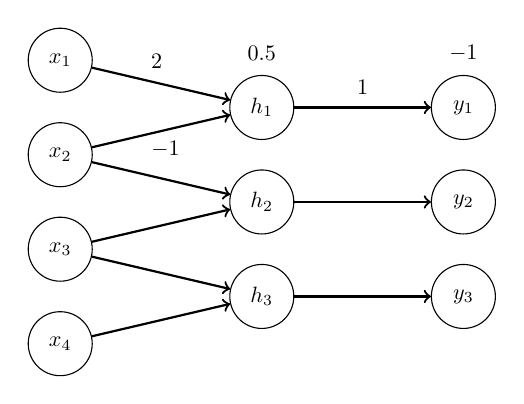
\begin{tikzpicture}[scale=0.8, transform shape]
    % Parameters
    \def\inpN{4}
    \def\hidN{3}
    \def\outN{3}
    \def\dy{1.5}
    \def\xInput{0}
    \def\xHidden{3.2}
    \def\xOutput{6.4}

    % Input nodes
    \foreach \i [evaluate=\i as \lbl using int(\i)] in {1,...,4} {
        \node[circle, draw, fill=white, minimum size=0.4in, label=center:{$x_{\lbl}$}] 
            (I\i) at (\xInput, {(4-1)*0.5*\dy - (\i-1)*\dy}) {};
    }

    % Hidden nodes
    \node[circle, draw, fill=white, minimum size=0.4in, label=center:{$h_1$}] at (\xHidden, {1.5}) (H1) {};
    \node[above=0.1cm of H1] (B1) {$0.5$};
    \node[circle, draw, fill=white, minimum size=0.4in, label=center:{$h_2$}] at (\xHidden, {0}) (H2) {};
    % \node[above=0.2cm of H2] (B2) {$b=0.5$};
    \node[circle, draw, fill=white, minimum size=0.4in, label=center:{$h_3$}] at (\xHidden, {-1.5}) (H3) {};
    % \node[above=0.2cm of H3] (B3) {$b=0.5$};

    % Output nodes
    \node[circle, draw, fill=white, minimum size=0.4in, label=center:{$y_1$}] at (\xOutput, {1.5}) (O1) {};
    \node[above=0.1cm of O1] (B1) {$-1$};
    \node[circle, draw, fill=white, minimum size=0.4in, label=center:{$y_2$}] at (\xOutput, {0}) (O2) {};
    \node[circle, draw, fill=white, minimum size=0.4in, label=center:{$y_3$}] at (\xOutput, {-1.5}) (O3) {};

    % Connections: Input to Hidden (with weight labels spaced to avoid overlap)
    \draw[->, thick] (I1) -- node[above=2pt, midway, xshift=-2pt, yshift=1pt] {$2$} (H1);
    \draw[->, thick] (I2) -- node[below=1pt, midway, xshift=2pt] {$-1$} (H1);
    \draw[->, thick] (I2) -- (H2);
    \draw[->, thick] (I3) -- (H2);
    \draw[->, thick] (I3) -- (H3);
    \draw[->, thick] (I4) -- (H3);

    % Hidden to Output, one to one
    \draw[->, thick] (H1) -- node[above=2pt, midway] {$1$} (O1);
    \draw[->, thick] (H2) -- (O2);
    \draw[->, thick] (H3) -- (O3);

    \end{tikzpicture}
    \caption{1-dimensional CNN}\label{fig:cnn}
\end{figure}

\begin{example}
    \autoref{fig:cnn} shows a simple CNN with four inputs, three hidden neurons, and three outputs. %The first hidden neuron computes a weighted sum of its inputs, applies the ReLU activation function, and produces an output. The second and third hidden neurons compute their outputs similarly. The outputs are computed by taking the outputs of the hidden neurons and applying a linear transformation (without activation) to produce the final output values.
Given an input vector $\mathbf{x} = [x_1, x_2, x_3, x_4]$, the computation of the first output proceeds as follows. 
The first hidden unit forms a linear combination of its inputs as $h_1 = 2x_1 - x_2 + 0.5$. 
This value is then passed through the ReLU activation function, resulting in $\hat{h}_1 = \mathrm{ReLU}(h_1) = \max(0, 2x_1 - x_2 + 0.5)$. 
Finally, the first output is simply $y_1 = \hat{h}_1 - 1$.


\end{example}

\paragraph{Residual Networks (ResNets)} Resnets extend FNNs by adding \emph{skip connections}—direct links that bypass one or more layers. Resnets are often used in image recognition and classification. 

\begin{example}
\begin{figure}[htp]
    \centering
    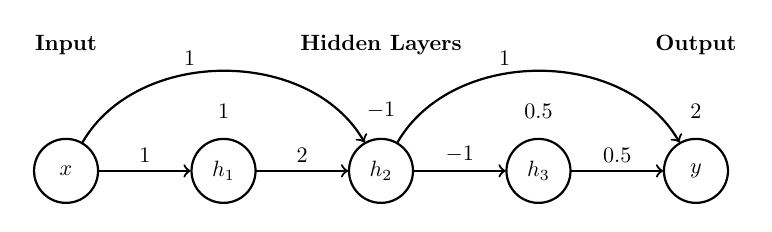
\begin{tikzpicture}[scale=0.8, transform shape]
    % Horizontal node positions with labels
    \node[circle, draw=black, thick, minimum size=0.4in, fill=white, label=center:{$x$}] (H1) at (0,0) {};
    \node[circle, draw=black, thick, minimum size=0.4in, fill=white, label=center:{$h_1$}] (H2) at (2.5,0) {};
    \node[circle, draw=black, thick, minimum size=0.4in, fill=white, label=center:{$h_2$}] (H3) at (5,0) {};
    \node[circle, draw=black, thick, minimum size=0.4in, fill=white, label=center:{$h_3$}] (H4) at (7.5,0) {};
    \node[circle, draw=black, thick, minimum size=0.4in, fill=white, label=center:{$y$}] (H5) at (10,0) {};

    % Layer labels
    \node at (0,2.0) {\textbf{Input}};
    \node at (5.0,2.0) {\textbf{Hidden Layers}};
    \node at (10.0,2.0) {\textbf{Output}};

    % Biases above all except input node
    \node[above=0.18cm of H2] {$1$};    % bias for h1
    \node[above=0.18cm of H3] {$-1$}; % bias for h2
    \node[above=0.18cm of H4] {$0.5$};  % bias for h3
    \node[above=0.18cm of H5] {$2$};    % bias for y

    % Main arrows with weights
    \draw[->, thick] (H1) -- node[above, midway] {$1$} (H2);
    \draw[->, thick] (H2) -- node[above, midway] {$2$} (H3);
    \draw[->, thick] (H3) -- node[above, midway] {$-1$} (H4);
    \draw[->, thick] (H4) -- node[above, midway] {$0.5$} (H5);

    % Residual (skip) connections with weights
    \draw[->, thick] (H1) to[out=60,in=120] node[above, pos=0.4] {$1$} (H3);
    \draw[->, thick] (H3) to[out=60,in=120] node[above, pos=0.4] {$1$} (H5);

    \end{tikzpicture}
    \caption{ResNet block with weights on all connections and biases above nodes. Each node is labeled and typical ReLU is applied after each hidden sum.}\label{fig:resnet}
\end{figure}


\autoref{fig:resnet}  shows an example of a Resnet.
Assume the input $x$ and each node applies the ReLU activation. With the weights and biases shown in the diagram, the outputs are computed as follows:

\[
\begin{aligned}
    h_1 = \relu{x + 1} &\quad h_2 = \relu{2h_1 + x - 1} \\
    h_3 = \relu{-h_2 + 0.5} &\quad y  = 0.5h_3 + h_2 + 2
\end{aligned}
\]

\end{example}

% \subsubsection*{Common Layer Types}

% Feedforward networks, including CNNs and ResNets, are built from layers such as:

% \begin{itemize}
%     \item \textbf{Fully Connected (Dense) Layers}: Every neuron is connected to every neuron in the next layer.
%     \item \textbf{Convolutional Layers}: Local filters scan over inputs to extract spatial features.
%     \item \textbf{Residual (Skip) Connections}: Enable shortcut paths from earlier to later layers.
% \end{itemize}

\subsection{Other NN Architectures}

Not all NNs are feedforward. Some architectures introduce cycles, dynamic connections, or non-Euclidean data structures.

\paragraph{Recurrent Neural Networks (RNNs)} RNNs, often used in natural language process and speech recognition, are designed to recognize patterns in sequences of data. RNNs have \emph{loops} in them, allowing information to be sent forward and backward.


\begin{figure}[h]
    \begin{center}
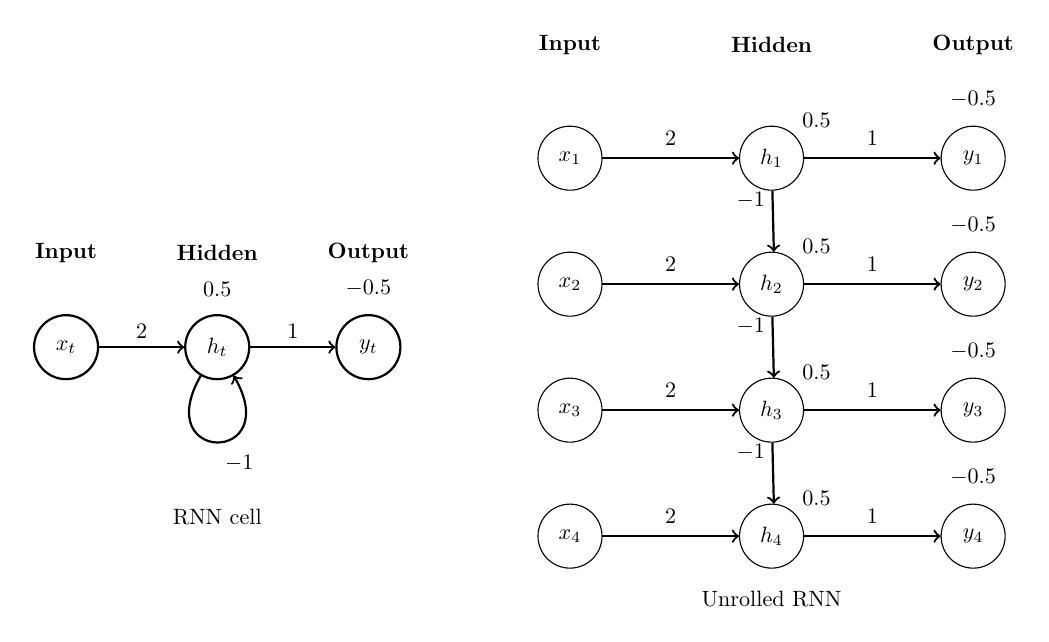
\begin{tikzpicture}[scale=0.8, transform shape]
% --- Rolled RNN (left diagram) ---
\begin{scope}
% Layer labels
\node at (0,1.5) {\textbf{Input}};
\node at (2.4,1.5) {\textbf{Hidden}};
\node at (4.8,1.5) {\textbf{Output}};
% Nodes
\node[circle, draw=black, fill=white, thick, minimum size=0.4in, label=center:{$x_t$}] (RI) at (0,0) {};
\node[circle, draw=black, fill=white, thick, minimum size=0.4in, label=center:{$h_t$}] (RH) at (2.4,0) {};
\node[circle, draw=black, fill=white, thick, minimum size=0.4in, label=center:{$y_t$}] (RO) at (4.8,0) {};
% Bias above nodes
\node[above=0.16cm of RH] {$0.5$};
\node[above=0.16cm of RO] {$-0.5$};
% Main arrows with weights
\draw[->, thick] (RI) -- node[above, pos=0.5] {$2$} (RH);
\draw[->, thick] (RH) -- node[above, pos=0.5] {$1$} (RO);
% Recurrent/self-loop at hidden node with recurrent weight
\draw [->, thick] (RH) edge [out=-120,in=-60,looseness=8] node[below, yshift=-2pt, xshift=10pt] {$-1$} (RH);
% Caption
\node[align=center] at (2.4,-2.7) {RNN cell};
\end{scope}



% --- Unrolled RNN (right diagram) ---
\begin{scope}[xshift=8cm]
% Parameters for vertical node spacing
\def\inpN{4}
\def\hidN{4}
\def\outN{4}
\def\dy{2.0}
\def\xInput{0}
\def\xHidden{3.2}
\def\xOutput{6.4}
% Layer labels
\node at (\xInput,{\inpN/2*\dy+0.8}) {\textbf{Input}};
\node at (\xHidden,{\inpN/2*\dy+0.8}) {\textbf{Hidden}};
\node at (\xOutput,{\inpN/2*\dy+0.8}) {\textbf{Output}};
% Input nodes (left column)
\foreach \i in {1,...,\inpN} {
    \node[circle, draw=black, fill=white, minimum size=0.4in, label=center:{$x_{\i}$}] (I\i) at (\xInput, {(\inpN-1)*0.5*\dy - (\i-1)*\dy}) {};
}
% Hidden nodes (centered) (as many as input)
\foreach \i in {1,...,\hidN} {
    \node[circle, draw=black, fill=white, minimum size=0.4in, label=center:{$h_{\i}$}] (H\i) at (\xHidden, {(\hidN-1)*0.5*\dy - (\i-1)*\dy}) {};
    \node[above right=0 of H\i] {$0.5$}; % Bias above each hidden
}
% Output nodes (centered) (as many as input)
\foreach \i in {1,...,\outN} {
    \node[circle, draw=black, fill=white, minimum size=0.4in, label=center:{$y_{\i}$}] (O\i) at (\xOutput, {(\outN-1)*0.5*\dy - (\i-1)*\dy}) {};
    \node[above=0.16cm of O\i] {$-0.5$}; % Bias above each output
}
% RNN input-to-hidden (1-to-1, with weight)
\foreach \i in {1,...,4} {
    \draw[->, thick] (I\i) -- node[above, pos=0.5, yshift=2pt] {$2$} (H\i);
}
% Hidden-to-hidden (recurrent arrows, with weight)
\foreach \i [evaluate={\j=int(\i+1);}] in {1,2,3} {
    \draw[->, thick] ([xshift=4pt]H\i) -- node[above left, pos=0.5, yshift=2pt] {$-1$} ([xshift=-4pt]H\j);
}
% Hidden-to-output (1-to-1, with weight)
\foreach \i in {1,...,4} {
    \draw[->, thick] (H\i) -- node[above, pos=0.5, yshift=2pt] {$1$} (O\i);
}
% Caption
\node[align=center] at (3.2,-4.0) {Unrolled RNN};
\end{scope}
\end{tikzpicture}
\end{center}
\caption{RNN cell (left) and unrolled RNN sequence structure (right). 
Weights on connections; biases above hidden and output nodes.}
\label{fig:rnn}
\end{figure}

\begin{example}
\autoref{fig:rnn} shows a simple RNN cell. Assume the input sequence is $\mathbf{x} = [x_1, x_2, x_3, x_4]$, and the initial hidden state is $h_0$. 
For the first time step, the hidden state is computed as $h_1 = \relu{2x_1 - h_0 + 0.5}$, and the output is $y_1 = h_1 - 0.5$. 
For the second time step, the hidden state is $h_2 = \relu{2x_2 - h_1 + 0.5}$, and the output is $y_2 = h_2 - 0.5$.
% For the third time step, the hidden state is $h_3 = ReLU(2x_3 - h_2 + 0.5)$, and the output is $y_3 = h_3 - 0.5$.
% For the fourth time step, the hidden state is $h_4 = ReLU(2x_4 - h_3 + 0.5)$, and the output is $y_4 = h_4 - 0.5$.

\end{example}

\paragraph{Transformers} are designed for long-range dependencies using \emph{self-attention} rather than recurrence. They dominate applications in natural language processing and are increasingly used in vision and reinforcement learning.

\paragraph{Graph Neural Networks (GNNs)} operate on graphs, allowing each node to aggregate information from its neighbors. They are used in applications involving structured data like molecules or social networks.



\section{ONNX: Modelling Neural Networks}\label{sec:onnx}

\textbf{ONNX} (Open Neural Network Exchange)~\cite{onnx} is an open source and widely adopted standard for representing neural networks. It provides a common format for representing the structure and parameters of neural networks, enabling interoperability between different ML frameworks and tools.

%\paragraph{Supported ONNX Operators} VNN-LIB supports a subset of ONNX operators that cover most sequential feedforward networks used in NN verification. These operators include:


ONNX operators that cover most sequential feedforward networks include: 
\begin{itemize}
    \item \texttt{Add, Sub, Gemm, MatMul}: basic arithmetic and matrix operations.
    \item \texttt{ReLU, Sigmoid, SoftMax}: activation functions.
    \item \texttt{AveragePool, MaxPool, Flatten, Reshape}: tensor manipulation.
    \item \texttt{Conv, BatchNormalization, LRN}: CNN layers and normalizations.
    \item \texttt{Concat, Dropout, Unsqueeze}: tensor operations.
\end{itemize}

%\textbf{Note:} Preprocessing (e.g., normalization) should not be included in the model itself to keep property alignment clear.

\begin{example} For the network in \autoref{fig:dnn}, the ONNX representation would include:
\begin{itemize}
    \item Input: $x_1, x_2$.
    \item Hidden layer: $x_3 = \relu{-0.5x_1 + 0.5x_2 + 1.0}$, $x_4 = \relu{0.5x_1 - 0.5x_2 + 1.0}$.
    \item Output: $x_5 = -x_3 + x_4 - 1$.
\end{itemize} 
The ONNX representation would look like:\tvn{could we put in the exact ONNX code?}\hd{working on it}

\begin{lstlisting}[basicstyle=\ttfamily\scriptsize]
(opset_version 13)
(node (name "input") (op_type "Input") (inputs) (outputs ("x1" "x2")))
(node (name "hidden1") (op_type "ReLU") (inputs ("x1" "x2")) (outputs ("x3")))
(node (name "hidden2") (op_type "ReLU") (inputs ("x1" "x2")) (outputs ("x4")))
(node (name "output") (op_type "Add") (inputs ("x3" "x4")) (outputs ("x5")))
\end{lstlisting}

\hai{ONNX onnx.helper.printable\_graph}

\begin{lstlisting}[basicstyle=\ttfamily\scriptsize]
graph torch_jit (
  %onnx::Flatten_0[FLOAT, 1x2]
) initializers (
  %1.weight[FLOAT, 3x2]
  %1.bias[FLOAT, 3]
  %3.weight[FLOAT, 4x3]
  %3.bias[FLOAT, 4]
  %5.weight[FLOAT, 2x4]
  %5.bias[FLOAT, 2]
) {
  %onnx::Gemm_7 = Flatten[axis = 1](%onnx::Flatten_0)
  %input = Gemm[alpha = 1, beta = 1, transB = 1](%onnx::Gemm_7, %1.weight, %1.bias)
  %onnx::Gemm_9 = Relu(%input)
  %input.3 = Gemm[alpha = 1, beta = 1, transB = 1](%onnx::Gemm_9, %3.weight, %3.bias)
  %onnx::Gemm_11 = Relu(%input.3)
  %12 = Gemm[alpha = 1, beta = 1, transB = 1](%onnx::Gemm_11, %5.weight, %5.bias)
  return %12
}
\end{lstlisting}


\hai{ONNX raw model (need to update weights to match the example)}

\begin{lstlisting}[basicstyle=\ttfamily\scriptsize]
    ir_version: 7
    producer_name: "pytorch"
    producer_version: "1.12.1"
    graph {
      node {
        input: "onnx::Flatten_0"
        output: "onnx::Gemm_7"
        name: "Flatten_0"
        op_type: "Flatten"
        attribute {
          name: "axis"
          i: 1
          type: INT
        }
      }
      node {
        input: "onnx::Gemm_7"
        input: "1.weight"
        input: "1.bias"
        output: "input"
        name: "Gemm_1"
        op_type: "Gemm"
        attribute {
          name: "alpha"
          f: 1.0
          type: FLOAT
        }
        attribute {
          name: "beta"
          f: 1.0
          type: FLOAT
        }
        attribute {
          name: "transB"
          i: 1
          type: INT
        }
      }
      node {
        input: "input"
        output: "onnx::Gemm_9"
        name: "Relu_2"
        op_type: "Relu"
      }
      node {
        input: "onnx::Gemm_9"
        input: "3.weight"
        input: "3.bias"
        output: "input.3"
        name: "Gemm_3"
        op_type: "Gemm"
        attribute {
          name: "alpha"
          f: 1.0
          type: FLOAT
        }
        attribute {
          name: "beta"
          f: 1.0
          type: FLOAT
        }
        attribute {
          name: "transB"
          i: 1
          type: INT
        }
      }
      node {
        input: "input.3"
        output: "onnx::Gemm_11"
        name: "Relu_4"
        op_type: "Relu"
      }
      node {
        input: "onnx::Gemm_11"
        input: "5.weight"
        input: "5.bias"
        output: "12"
        name: "Gemm_5"
        op_type: "Gemm"
        attribute {
          name: "alpha"
          f: 1.0
          type: FLOAT
        }
        attribute {
          name: "beta"
          f: 1.0
          type: FLOAT
        }
        attribute {
          name: "transB"
          i: 1
          type: INT
        }
      }
      name: "torch_jit"
      initializer {
        dims: 3
        dims: 2
        data_type: 1
        name: "1.weight"
        raw_data: "\020\204\t\277\177\231\302>g\022\030\277\343\222\346=\226\037\327>TR\367\276"
      }
      initializer {
        dims: 3
        data_type: 1
        name: "1.bias"
        raw_data: "HT\n?K\024\224>\252\\\000\272"
      }
      initializer {
        dims: 4
        dims: 3
        data_type: 1
        name: "3.weight"
        raw_data: "\007l\212\274I\023\006?\261B:>j.\247>1\302\221\276\361\\\036>\357~\206\276o\000\326>\013\345\260\2731\260%\276\006\242\272\276\367\331\373\276"
      }
      initializer {
        dims: 4
        data_type: 1
        name: "3.bias"
        raw_data: "\311\360\304=S\346-<\236\024\251\276U /\276"
      }
      initializer {
        dims: 2
        dims: 4
        data_type: 1
        name: "5.weight"
        raw_data: "\370\222\342\275\200w\336<\004A\273\276\000;\023>hz\246=@\221\327<j\222\266>\342\014\325>"
      }
      initializer {
        dims: 2
        data_type: 1
        name: "5.bias"
        raw_data: "\024\256{\276,/\205\276"
      }
      input {
        name: "onnx::Flatten_0"
        type {
          tensor_type {
            elem_type: 1
            shape {
              dim {
                dim_value: 1
              }
              dim {
                dim_value: 2
              }
            }
          }
        }
      }
      output {
        name: "12"
        type {
          tensor_type {
            elem_type: 1
            shape {
              dim {
                dim_value: 1
              }
              dim {
                dim_value: 2
              }
            }
          }
        }
      }
    }
    opset_import {
      version: 13
    }
\end{lstlisting}

\end{example}






% \begin{figure}[htp]
%     \begin{center}
%     \begin{tikzpicture}[scale=0.8, transform shape]
%         % --- Rolled RNN (left diagram) ---
%         \begin{scope}
%             % Layer labels
%             \node at (0,1.5) {\textbf{Input}};
%             \node at (2.4,1.5) {\textbf{Hidden}};
%             \node at (4.8,1.5) {\textbf{Output}};
%             % Nodes
%             \node[circle, draw=black, fill=white, thick, minimum size=0.4in] (RI) at (0,0) {};
%             \node[circle, draw=black, fill=white, thick, minimum size=0.4in] (RH) at (2.4,0) {};
%             \node[circle, draw=black, fill=white, thick, minimum size=0.4in] (RO) at (4.8,0) {};
%             % Main arrows
%             \draw[->, thick] (RI) -- (RH);
%             \draw[->, thick] (RH) -- (RO);
%             % Recurrent/self-loop at hidden node
%             \draw [->, thick] (RH) edge [out=-120,in=-60,looseness=8] (RH);
%             % Caption
%             \node[align=center] at (2.4,-1.7) {Rolled RNN};
%         \end{scope}
        
%         % --- Unrolled RNN (right diagram) ---
%         \begin{scope}[xshift=8cm]





% \section{Properties of Neural Networks}

% \paragraph{Robustness Properties}
% \emph{Robustness}, a desirable property for all networks, ensures that small perturbations in the input data do not cause major changes in the output of the network. For example, if a few pixels in an image are changed, the network should still classify the image correctly. \emph{Adversarial attacks} are a common way to test the robustness of a neural network. In an adversarial attack, an attacker makes small changes to the input data to cause the network to misclassify the data.

% \emph{Local} robustness refers to robustness of a neural network within a \emph{small neighborhood or region} of the input data. In contrast, \emph{global} robustness refers to robustness of a network across the \emph{entire input space}. Global robustness is harder to achieve than local robustness, as it requires the network to be robust to all possible inputs.

% \paragraph{$\epsilon$-robustness} A neural network is $\epsilon$-robust if the difference between any two inputs $x$ and $x'$ is within a small range $\epsilon$, the output $f$ of the network does not change significantly (or remain the same), i.e., $\|x-x'\| \leq \epsilon \implies f(x) \approx f(x')$.


\chapter{Properties}\label{chap:properties}

Similar to software programs, neural networks (NNs) have desirable properties to ensure the network behaves as expected. These could be specific to the applications modeled by the network, e.g., safety properties for a network modelling a collision avoidance system, or general properties that are desired by all networks, e.g., robustness to small perturbations in the input data.

Below we will discuss properties that are relevant to the verification of NNs. Specifically, these properties can be 
expressed in a formal language supported by a DNN verifier. Additional properties can be found in the literature~\cite{seshia2018formal}.

\section{Properties, Informally}

As described in~\autoref{sec:basic} NNs define functions of the form $f: \mathbb{R}^{n} \to \mathbb{R}^{m}$, 
where $n$ is the dimension of the input and $m$ is the dimension of the output. Thus, the properties (or specifications) of an NN---similarly to properties of software program---are defined in terms of its input and output:

\begin{quote}
\textit{For any input $x \in \mathbb{R}^{n}$ satisfying a precondition $P$, the neural network should produce an output $f(x) \in \mathbb{R}^{m}$ that satisfies a postcondition $Q$.}
\end{quote}

This says that if the input $x$ satisfies the precondition $P$, then the output $f(x)$ should satisfy the postcondition $Q$.






\section{Common Properties in Neural Networks}

We now define some commonly studied correctness properties in NNs verification.

\subsection{Robustness}

\textbf{Robustness} ensures that small changes in the input do not drastically change the output. This is a desirable property for all neural networks, especially classifiers, where we want to ensure that similar inputs yield similar outputs. For example, a slightly blurred image of a red light should still be classified as a red light.

\begin{example}[Image Classification]
Consider a neural network $f$ that classifies images into different categories (e.g., dog, cat, etc.). Robustness requires that if an input image $c$ is classified as a dog, then any perturbed image $x$ that is visually similar to $c$ should also be classified as a dog. This can be expressed as:

\[
\|x - c\| \leq \epsilon \implies f(x) = f(c), 
\]
where $\|x - c\| \leq \epsilon$ indicates that the difference between the two images is within a certain (small) threshold, which is typically defined in terms of pixel-wise differences.
\end{example}

%Here, $\epsilon$ defines the perturbation bound, and the norm $\|\cdot\|$ is typically the $L_\infty$ norm, which captures the maximum pixel-wise change in the image.\tvn{what's the norm? and $L_\infty$?}


\subsection{Safety}


\textbf{Safety} ensures that the network conforms to certain safety constraints, often specific to the application domain. This is particularly important in safety-critical applications, such as autonomous vehicles or medical diagnosis systems, where incorrect outputs can lead to catastrophic consequences. For example, in a self-driving car, we want to ensure that the car maintains a safe distance from other vehicles and pedestrians under all scenarios.

\begin{example}[Collision Avoidance System]
    A safety property in a collision avoidance system such as an autonomous vehicle might be that if the intruder is distant and significantly slower than us, then we stay below a certain velocity threshold. Formally, this can be expressed as:
\[
d_{intruder} > d_{threshold} \land v_{intruder} < v_{threshold} \implies v_{us} < v_{threshold},
\]
where $d_{intruder}$ is the distance to the intruder, $d_{threshold}$ is a predefined safe distance, $v_{intruder}$ is the speed of the intruder, and $v_{us}$ is our speed.
\end{example}

\section{Other properties}\label{sec:other-properties}

\subsection{Consistency}

\textbf{Consistency} ensures that a neural network behaves in a logically coherent manner, maintaining stable and predictable outputs under semantically equivalent or related inputs. This property requires that the network's predictions follow logical relationships and respect domain-specific invariants, preventing contradictory outputs that would violate fundamental assumptions of the problem domain. 

\begin{example}[Logical Consistency in Large Language Models]
    A consistency property in an LLM-based question answering system requires that the model provides logically coherent answers to related questions. For instance, given a set of related queries about the same factual information, the model should maintain consistency. Formally, consider queries $q_1$, $q_2$, and $q_3$ about a person's age:
\[
q_1: \text{"How old is person X?"}
\]
\[
q_2: \text{"What year was person X born if they are currently Y years old?"}
\]
\[
q_3: \text{"Will person X be Z years old in 2025?"}
\]
The consistency property requires that if the LLM outputs age $Y$ for $q_1$, then the birth year in $q_2$ should be $\text{current\_year} - Y$, and the answer to $q_3$ should be logically consistent with the stated age. This prevents scenarios where an LLM claims someone is 30 years old but was born in 1985 when the current year is 2024, ensuring logical coherence across related factual queries.
\end{example}


% \paragraph{Example: Object Position Consistency.}
% Consider a neural network tracking the position of objects in a video frame. It should not report that an object is on the left in one frame and then immediately claim it is on the right in the next frame.

% \paragraph{Formal Specification:}
% \[
% \{ \text{frame } t, \text{ frame } t+1 \}
% \quad r_1 \gets f(x_t), \quad r_2 \gets f(x_{t+1})
% \quad \{ \text{consistent}(r_1, r_2) \}
% \]

\subsection{Monotonicity}

\textbf{Monotonicity} ensures that the neural network maintains a consistent ordering relationship between inputs and outputs, where an increase in certain input features always leads to a non-decreasing output value. This property is particularly important in applications where domain knowledge dictates logical ordering constraints, such as fairness-aware systems, medical diagnosis, and scientific applications where physical laws impose natural ordering relationships.

\begin{example}[Fairness]
    A monotonicity property in an AI system should ensure that relevant merit-based features are monotonic while demographic features like gender have no effect on the outcome. For instance, in a university admissions system, the admission probability should be monotonically non-decreasing with respect to GPA and test scores, regardless of gender. Formally, for applicants with profiles $(p, s, g)$ and $(p', s', g')$ where $p, p'$ are GPAs, $s, s'$ are test scores, and $g, g'$ are gender indicators:
\[
p \leq p' \land s = s' \land g \neq g' \implies f(p, s, g) \leq f(p', s', g'),
\]
\[
s \leq s' \land p = p' \land g \neq g' \implies f(p, s, g) \leq f(p, s', g'),
\]
where $f$ is the neural network computing admission probability. Additionally, for gender fairness:
\[
f(p, s, \text{male}) = f(p, s, \text{female}) \text{ for all } p, s,
\]
ensuring that applicants with identical academic qualifications receive the same treatment regardless of gender, while maintaining logical ordering based on academic merit.
\end{example}



\section{Counterexamples}\label{sec:counterexamples}

A \emph{counterexample} (\textbf{cex}) is a witness that falsifies the correctness property. A counterexample is an assignment to the input variables that satisfies the precondition but violates the postcondition.

\begin{example}[Counterexample to Robustness Property]
For the brightness robustness property:
\[
\text{If } f(x) \neq f(c) \text{ and } \|x - c\| \leq \epsilon, \text{ then } x \text{ is a counterexample.}
\]
\end{example}


\section{The VNN-LIB  Specification Language}


The VNN-LIB standard~\cite{demarchi2023supporting,vnnlib} defines a format to describe neural networks and properties. Such a standard format enables the sharing of benchmarks across different tools and platforms, facilitating evaluations and comparisons of their performance. The international VNN-COMP competition~\cite{brix2024fifth} also uses VNN-LIB to evaluate the performance of different neural network verification tools.


Specifically, VNN-LIB defines a common format for the following components:
\begin{itemize}
    \item \textbf{Neural Network (or model) representation} in the ONNX format~\cite{onnx}.
    \item \textbf{Property specification} in SMT-LIB format~\cite{barrett2010smt}.
\end{itemize}



\subsection{VNN-LIB: Property Specification Language}

Verification tasks involve proving that the output of a network remains within some desired post-condition $\Sigma$, given inputs within a bounded set $\Pi$.

\paragraph{Formal Specification}
Let $\nu: D^{n_1 \times \dots \times n_h} \to D^{m_1 \times \dots \times m_k}$ be a neural network, and $x$ and $y$ its input and output tensors. A property is expressed as:
\[
\forall x \in \Pi \rightarrow \nu(x) \in \Sigma
\]
This includes:
\begin{itemize}
    \item \textbf{Precondition} $\Pi$: constraints on inputs.
    \item \textbf{Postcondition} $\Sigma$: required properties of outputs.
\end{itemize}

Properties are encoded in \textbf{SMT-LIB2}, referencing input/output variable names consistent with ONNX.


\begin{example}[ACAS XU Network]

A typical ACAS XU network (\autoref{sec:acasxu}) maps 5D input to 5D output via 6 layers of 50 ReLU neurons. A local robustness property is:
\[
-\varepsilon_i \leq x_i \leq \varepsilon_i \quad (0 \leq i < 5)
\]
\[
y_0 \leq y_1, \quad y_0 \leq y_2, \quad y_0 \leq y_3, \quad y_0 \leq y_4
\]

The VNN-LIB code for this property is as follows:

\begin{lstlisting}[style=SMTLIB-style, language=SMTLIB,basicstyle=\ttfamily\scriptsize]

; declaring the input variables
(declare-const X_0 Real)
(declare-const X_1 Real)
(declare-const X_2 Real)
(declare-const X_3 Real)
(declare-const X_4 Real)
(declare-const X_5 Real)

; declaring neuron outputs
(declare-const Y_0 Real)
(declare-const Y_1 Real)
(declare-const Y_2 Real)
(declare-const Y_3 Real)
(declare-const Y_4 Real)

; asserting the input relations
(assert (<= X_0 eps0))
(assert (>= X_0 -eps0))
(assert (<= X_1 eps1))
(assert (>= X_1 -eps1))
(assert (<= X_2 eps2))
(assert (>= X_2 -eps2))
(assert (<= X_3 eps3))
(assert (>= X_3 -eps3))
(assert (<= X_4 eps4))
(assert (>= X_4 -eps4))

; asserting the output relations
(assert (<= Y_0 Y_1))
(assert (<= Y_0 Y_2))
(assert (<= Y_0 Y_3))
(assert (<= Y_0 Y_4))
\end{lstlisting}
\end{example}


% \begin{example}[MNIST Network]

% A CNN model for MNIST uses:
% \begin{itemize}
%     \item 2 convolutional layers (5x5 kernel, padding 2), followed by ReLU and MaxPool (2x2).
%     \item A flatten layer, then a fully connected layer with 10 outputs.
%     \item Input: $1 \times 28 \times 28$; Output: 10-class classification.
% \end{itemize}

% A robustness property around a sample $\hat{x}$ classified as class 9:
% \[
% \forall i \in [0, 783] : \hat{x}_i - \varepsilon \leq x_i \leq \hat{x}_i + \varepsilon
% \]
% \[
% \forall j \in [0,8] : y_j - y_9 \leq 0
% \]


% \subsubsection*{Variable Naming Convention}\tvn{what's the purpose of this section?}\hd{seems unnecessary}
% \begin{itemize}
%     \item 1D tensor: \texttt{X\_0, X\_1, ..., X\_n}
%     \item 2D tensor: \texttt{X\_0-0, X\_0-1, ..., X\_n-m}
%     \item 3D tensor: \texttt{X\_0-0-0, ..., X\_i-j-k}
% \end{itemize}

% \paragraph{Example: Tensor Flattening Algorithm}
% \begin{lstlisting}
% procedure flatten(x)
%     idx = 0
%     for a = 0 to N1
%       for b = 0 to N2
%         ...
%           for k = 0 to Nk
%             X_idx = x[a][b]...[k]
%             idx += 1
% \end{lstlisting}

% \noindent In SMT-LIB:
% \begin{lstlisting}
% (declare-fun X0 () Real) ; or (declare-fun X_0-0-0 () Real)
% ...
% (assert (<= X0 (+ Xhat0 eps)))
% (assert (>= X0 (- Xhat0 eps)))
% ...
% (assert (<= (- FC0_0 FC0_9) 0.0))
% \end{lstlisting}








\chapter{Verification of Neural Networks}\label{sec:verification}


\section{The Neural Network Verification (NNV) Problem}\label{sec:nnv-problem}

\begin{definition}[NNV]
Given a DNN \(N\) and a property $\phi$, the \emph{DNN verification problem} asks if $\phi$ is a valid property of $N$.
Typically, $\phi$ is a formula of the form $\phi_{in} \Rightarrow \phi_{out}$, where $\phi_{in}$ is a property over the inputs of $N$ and $\phi_{out}$ is a property over the outputs of $N$.
%This form of properties has been used to encode safety and security requirements of DNNs, e.g., safety specifications to avoid collision in unmanned aircraft~\cite{kochenderfer2012next} and \emph{adversarial robustness}~\cite{katz2017towards} properties desired by all DNNs, in which a small input perturbation does not cause major spikes in the DNN's outputs.
A DNN verifier attempts to find a \emph{counterexample} input to $N$ that satisfies $\phi_{in}$ but violates $\phi_{out}$.  If no such counterexample exists, $\phi$ is a valid property of $N$. Otherwise, $\phi$ is not valid and the counterexample can be used to retrain or debug the DNN~\cite{huang2017safety}.
\end{definition}


% Verification tool such as Marabou and nnenum are then applied to the network to prove that the network is safe or identifier counterexample representing small input differences causing large output changes.


% \footnote{This is encoded as the differences of the inputs being within a certain small range  ($\phi_{in}$) implies the differences of the outputs still fall within a certain range in $\phi_{out}$)}.


\begin{example}\label{ex:dnn}
A \emph{valid} property for the DNN in \autoref{fig:dnn} is that the output is $x_5 \le 0$ for any inputs $x_1 \in [-1,1], x_2\in[-2,2]$. 

An \emph{invalid} property is that $x_5 > 0$ for those similar inputs.
A counterexample showing this property violation is $\{x_1=-1, x_2=2\}$, from which the DNN evaluates to $x_5=-3.5$. 
\end{example}

%Such properties can capture \emph{safety requirements} (e.g., a rule in an  collision avoidance system in~\cite{kochenderfer2012next,katz2017reluplex} is ``if the intruder is distant and significantly slower than us, then we stay below a certain threshold'') or \emph{local robustness}~\cite{katz2017towards} conditions (a form of adversarial robustness stating that small perturbations of a given input all yield the same output).


\section{Satisfiability Formulation}\label{sec:satisfiability-and-activation-pattern-search}

As with traditional software verification, DNN verification is often represented as a satisfiability problem, and check if a given property is satisfied by the DNN. 

To do this, we first need to define a formula $\alpha$ to represent the network. Typically $\alpha$ is a conjunction ($\bigwedge$) of constraints representing the affine transformation (\autoref{sec:affine}) and activation function (\autoref{sec:activation}) of each neuron in the network.
For example, for a fully-connected neural network (\autoref{sec:ffn}) with $L$ layers, $N$ ReLU neurons per layer, this formula is:

\begin{align*}
\alpha = &\bigwedge_{\begin{smallmatrix}i \in [1,L]\\ j \in [1,N]\end{smallmatrix}}~~v_{i,j} \equiv ReLU \Big( \sum_{k \in [1,N]} (w_{i-1,j,k} \cdot v_{i-1,j}) + b_{i,j}\Big)    \\
 = &\bigwedge_{\begin{smallmatrix}i \in [1,L]\\ j \in [1,N]\end{smallmatrix}}~~v_{i,j} \equiv \max \Big( \sum_{k \in [1,N]} (w_{i-1,j,k} \cdot v_{i-1,j}) + b_{i,j}, 0 \Big)
\end{align*}

With this definition the NNV problem can be formulated as checking the validity of the following formula:
\begin{equation}\label{eq:nnv}
    \alpha \implies (\phi_{in} \implies \phi_{out}).
\end{equation}
This formula checks if the network $N$ satisfies (implies) the property $\phi$, where $\phi_{in}$ is a precondition on the inputs and $\phi_{out}$ is a postcondition on the outputs. This validity checking can be reduced to checking the satisfiability of the formula:

\begin{equation}\label{eq:prob}
  \alpha \land \phi_{in} \land \neg \phi_{out}
\end{equation}
If \autoref{eq:prob} is unsatisfiable, then $\phi$ is a valid property of $\mathcal{N}$. Otherwise, $\phi$ is not valid.  Moreover, we can extract a counterexample for the original problem from the satisfying assignment of \autoref{eq:prob}.

\begin{example}\label{ex:dnn-sat}
We represent the DNN in \autoref{fig:dnn} as a formula $\alpha$ as follows:
\begin{align*}
& x_3 = -0.5x_1 + 0.5x_2 + 1.0 ~\land~ \hat{x}_3 = \relu{x_3} ~\land \\
& x_4 = 0.5x_1 - 0.5x_2 + 1.0  ~\land~ \hat{x}_4 = \relu{x_4} ~\land \\
& x_5 = -\hat{x}_3 + \hat{x}_4 - 1.0,
\end{align*}
\noindent and the property $x_5 > 0$ for any inputs $x_1 \in [-1,1], x_2\in[-2,2]$ as:
\begin{equation*}
\phi_{in} = (-1 \le x_1 \le 1) \land (-1 \le x_2 \le 2); \qquad
\phi_{out} = (x_5 > 0)
\end{equation*}

We then check the satisfiability of $\alpha \land \phi_{in} \land \neg \phi_{out}$ using a constraint solver (e.g., an SMT solver).  In this case, the formula is satisfiable and the solver returns \sat{}, and we query the solver for a satisfying assignment to the input variables, e.g., $x_1=-1$ and $x_2=2$. This assignment is a counterexample (\autoref{sec:counterexamples}) to the property, as it satisfies the input constraint $\phi_{in}$ but violates the output constraint $\phi_{out}$, i.e., $x_5 = -3.5$, which is  $< 0$.

\end{example}

\section{Activation Pattern Search}\label{sec:activation-pattern}
 For ReLU-based DNNs, NNV becomes a search for \emph{activation patterns}, i.e., boolean assignments representing activation status of neurons, that lead to satisfaction the formula in \autoref{eq:prob}. 

Modern DNN verification techniques~\cite{bunel2020branch,wang2021beta,ferrari2022complete,duong2024harnessing,duong2023dpllt,ovalbab,katz2019marabou,bak2021nnenum} all adopt this idea and search for satisfying activation patterns.

\tvn{example of activation pattern search? using the above DNN example}
\hai{I will pull the example from our paper, but I think we also should create a tree to demonstrate how it proceeds -- I will work on this}


\tvn{Partial Activation Pattern}


\section{Complexity}\label{sec:complexity}

ReLU-based NNV is \NP{}-complete as shown in~\cite{katz2017reluplex,salzer2023reachability}. This means that the problem of checking whether a given ReLu-based DNN satisfies a property is computationally hard, and no polynomial-time algorithm is known to solve it in the general case.

\section{Challenges} %TODO

\subsection{Scalability} Neural networks can be very large, with millions of parameters. This makes it difficult to verify their correctness, as the number of possible inputs grows exponentially with the size of the network.

%TODO: put somewhere else  
For DNN verification, AF is straightforward to reason about because it is a linear function. However, AFs are often followed by non-linear activation functions, described next in \autoref{sec:activation}, which make the verification problem more challenging.

%TODO: put somewhere else
For DNN verification, these non-linear activation functions make verification difficult because it introduces multiple possible outcomes for any input, making it hard to reason about the output of the network. For example, ReLU has two possible outputs for any input: 0 if the input is less than zero, and the input itself otherwise, and Sigmoid has a smooth curve with infinite possible outputs for any input.


\subsection{Formalization}


\subsection{Expressiveness}



\section{Challenges in Specifying Properties}\tvn{TODO}

Specifying desirable properties for neural networks is not straightforward. Some challenges include:
\begin{itemize}
    \item \textbf{Incomplete Specifications:} We may not be able to specify all desirable properties.
    \item \textbf{Expressiveness} For tasks such as sentiment analysis or image recognition, functional correctness is hard to define precisely.
\end{itemize}



\part{Constraint Solving and Abstraction}

\chapter{Constraint Solving}\label{chap:constraint-solving}

\section{Symbolic Execution and SMT Solving}\label{sec:se-smt}

As described in~\autoref{sec:satisfiability-and-activation-pattern-search} the Neural Network Verification (NNV) problem can be represented as a satisfiability problem. Specifically, we encode the network $N$ as a logical formula $\alpha$, and use a constraint solver to check that $\alpha$ satisfies the property $\phi$ of interest.

A straightforward way to do this encoding is using \emph{symbolic execution} (SE)~\cite{baldoni2018survey,king1976symbolic}, a well-known software testing technique for finding bugs.  SE executes a program on symbolic inputs, i.e., inputs represented as symbols rather than concrete values, and tracks the reachability of program state as symbolic expressions, i.e., logical formulae over symbolic inputs. The satisfiability of these formulae is then checked using an SMT solver, and satisfying assignments represent inputs leading to the undesirable (buggy) program state.

\subsection{Symbolic Execution}\label{sec:se}
We can adapt traditional SE to our problem by treating the DNN as a program and neurons as variables and executing the DNN on symbolic inputs. Affine transformations can easily be represented as logical formulae because they are linear functions. Activation functions such as ReLUs are translated to disjunctions of linear functions or if-then-else statements, i.e., $\relu{x} ~=~ \max(x,0) ~=~ x \ge 0 \land x \lor 0 \land \neg x$.


\begin{example}\label{ex:se-dnn}
\begin{figure}
\centering
\mydnn
\caption{\label{fig:dnn-a}A simple DNN (similar to~\autoref{fig:dnn}).}
\end{figure}    

To create a logical formula representing the DNN in \autoref{fig:dnn-a}, we can symbolically execute the DNN on symbolic inputs $x_1,x_2$ and track the values of the neurons $x_3, x_4, x_5$ as a set (conjunction) of logical formulae.  SE starts with the inputs $x_1$ and $x_2$ and computes the values of the neurons in the hidden layer, $x_3$ and $x_4$, using the affine transformations, followed by ReLUs. Finally, SE computes the output neuron $x_5$ as a linear combination of the hidden layer neurons.

\begin{equation}\label{eq:se-dnn}
    \begin{split}
x_5 &= -x_3 + x_4 - 1.0 ~\land \\
x_3 &= \max(-0.5x_1 + 0.5x_2 + 1.0, 0) ~\land \\
x_4 &= \max(0.5x_1 - 0.5x_2 - 1.0, 0)
    \end{split}
\end{equation}

\end{example}

\subsection{SMT Solving}\label{sec:smt}
After obtaining the symbolic representation of the DNN, we can use an SMT solver~\cite{barrett2010smt} to check the satisfiability of the formula $\alpha \land \phi_{in} \land \neg \phi_{out} $, where $\alpha$ is the symbolic representation of the DNN, $\phi_{in}$ is the precondition on the inputs, and $\phi_{out}$ is the postcondition on the outputs. The solver checks if there exists an assignment to the symbolic inputs that satisfies the formula. If such an assignment exists, it means that the property is violated, and we can extract a counterexample from the satisfying assignment. Otherwise, if no such assignment exists, the property is valid



\begin{example}\label{ex:smt-dnn}
    To check that the DNN in~\autoref{fig:dnn-a} satisfies the property $x_5 > 0$ for any inputs $x_1 \in [-1,1], x_2\in[-2,2]$ (\autoref{ex:dnn-sat}), represented as:
\begin{align*}
\phi_{in} = (x_1 \ge -1) \land (x_1 \le 1) \land (x_2 \ge -2) \land (x_2 \le 2); \quad \phi_{out} = (x_5 > 0)
\end{align*}
We check the satisfiability of $\alpha \land \phi_{in} \land \neg \phi_{out}$:
\begin{align*}
\begin{split}
x_5 &= -x_3 + x_4 - 1.0 ~\land \\
x_3 &= \max(-0.5x_1 + 0.5x_2 + 1.0, 0) ~\land \\
x_4 &= \max(0.5x_1 - 0.5x_2 - 1.0, 0) ~\land \\
    &(x_1 \ge -1) \land (x_1 \le 1) \land (x_2 \ge -2) \land (x_2 \le 2) \quad \land
    (x_5 \le 0) \\
    \end{split}    
\end{align*}    

In this case, the SMT solver returns \sat{} and a satisfying assignment, e.g., $x_1=-1$ and $x_2=2$, which is a counterexample to the property. This means that for these inputs, the output $x_5 = -3.5$ violates the property $x_5 > 0$.
\end{example}

\subsection{Limitations}\label{sec:smt-limitations} 

While using symbolic execution and SMT solving is a straightforward way to verify DNNs, it has several practical limitations:
\begin{itemize}
    \item \textbf{Path Explosion and Scalability}: the number of paths that the solver has to analyze can grow exponentially with the number of ReLU-based neurons and layers as each ReLU, represented as a disjunction of linear functions, has two possible outputs for any input.  This leads to the notorious 
    \emph{path explosion} problem and becoming intractable for large DNNs.
    
    \item \textbf{Non-linearity:} Other non-linear activation functions (\autoref{sec:activation}), such as Sigmoid or Tanh, might not be easily representable as disjunctions of linear functions as ReLU. This can lead to complex formulae that are hard to reason about and/or result in a large search space for the SMT solver.
    
    \item \textbf{Precision Issues:} SMT solvers may struggle with precision issues when dealing with floating-point arithmetic, which is common in DNNs. This can lead to incorrect results or false positives/negatives in the verification process.
\end{itemize}

For these reasons, SMT solving is mostly used to demonstrate the correctness of small DNNs, e.g., in a classroom setting.  Modern-based DNN verification tools do not use SMT solving, and instead, rely on more efficient techniques including abstraction and MILP solving (\autoref{sec:milp}).

\tvn{Hai, include some references or results, e.g., from Nguyen's, showing that SMT solvers are not scalable for DNN verification.}\hai{where can I find the results?}\tvn{Not sure, I thought Nguyen record the results/graphs in some TeX document. Could you ask him?}

\section{MILP}\label{sec:milp}
Due to scalability issues with SMT solvers (\autoref{sec:smt-limitations}), modern DNN verification techniques ~\cite{wang2018efficient,tjeng2019evaluating,duong2024harnessing} often rely on Mixed Integer Linear Programming (MILP) solving, which is specialized for linear constraints and more efficient for DNN reasoning. %Many state-of-the-art DNN verification tools use the industrial-strength MILP solver Gurobi~\cite{gurobi}.

The fundamental distinction between SMT and MILP solving lies in their problem formulation and solution approach. 
SMT solvers address satisfiability problems: given a logical formula, determine whether there exist variable assignments that make the formula true. 
SMT solvers can handle diverse mathematical theories including non-linear arithmetic.
MILP solvers address optimization problems: find the best solution (according to some objective function) among all feasible solutions that satisfy a set of linear constraints. 
Note that MILP is restricted to linear constraints.

MILP solvers cannot directly solve general SMT problems because they are restricted to linear constraints and cannot handle the non-linear theories and complex logical structures that SMT problems often contain. 
While SMT solvers could theoretically encode MILP problems as satisfiability queries, they are not designed for optimization and would be highly inefficient. 
Despite both approaches having exponential worst-case complexity, MILP solvers often demonstrate superior practical performance due to their restriction to linear constraints, which enables several key optimizations such as linear relaxations, preprocessing techniques, and specialized algorithms. 


%\paragraph{MILP} Mixed Integer Linear Programming (MILP) is an optimization technique that solves problems involving both continuous variables (real numbers) and integer variables (including binary 0/1 variables), subject to linear constraints. Unlike SMT solvers that handle complex logical formulae with disjunctions, MILP solvers are specifically designed for linear constraints and can leverage decades of optimization research to solve large-scale problems efficiently.


\subsection{ReLU Encoding}\label{sec:relu-encoding}

To use MILP solving, we encode non-linear activation functions like ReLU using \emph{binary indicator} variables and linear constraints. For each neuron, we introduce a binary variable that indicates whether the neuron is ``active'' (output equals input) or ``inactive'' (output is zero). This transforms the non-linear $\max(x,0)$ operation into a set of linear inequalities controlled by the binary variable. 
We define 

\begin{itemize}
    \item $z$: the pre-activation value, i.e., the value that goes into ReLU
    \item $\hat{z}$: the post-activation value, i.e., the output of ReLU
    \item $a \in \{0,1\}$: a binary indicator variable encoding whether the neuron is active ($z \le 0$) or inactive ($z < 0$)
    \item $l, u$: lower and upper bounds on $z$ ($l \leq z \leq u$) over the input region 
\end{itemize}

The MILP encoding of $\hat{z} = \max(z, 0)$ is then:
\begin{align*}
    &\hat{z} \geq z \\
    &\hat{z} \geq 0 \\
    &\hat{z} \leq a \cdot u \\
    &\hat{z} \leq z - l(1-a) \\
    &a \in \{0,1\}
\end{align*}

These constraints enforce $\hat{z} = z$ when $a = 1$ (active, $z \geq 0$) and $\hat{z} = 0$ when $a = 0$ (inactive, $z < 0$), which capture the semantics of ReLU. Notice that these constraints are linear and involve both continuous variable $\hat{z}$ and binary variable $a$.



Note the importance of the upper and lower bounds $u$ and $l$ on $z$. These bounds are critical not only for making the MILP encoding tight, but also for ensuring that the binary indicator $a$ can only take on values that are valid given the possible range of $z$. For example, if $u < 0$, then $z$ can never be non-negative, so the active phase ($a=1$) is infeasible (the constraints are not satisfiable) and should be ruled out by the MILP encoding; similarly, if $l \geq 0$, only the active phase is possible. Being able to eliminate infeasible cases is crucial for the efficiency of the MILP solver, as it reduces the search space. In general, the tightness of the bounds $l$ and $u$ is crucial for the efficiency of the MILP solver and a major focus of DNN reasoning is developing techniques to capture these bounds more precisely (\autoref{chap:abstractions}).

\paragraph{Computing Bounds $l \le e \le u$}  To determine the pairs of values that achieve the lower and upper bounds of a linear expression $e$:
\[
 e = a_1 x_1 + a_2 x_2 + \ldots + b,
\]
where each variable $x_i$ ranges over $[l_i, u_i]$, we proceed as follow:

\begin{itemize}
    \item \textbf{For the lower bound} ($l_3$):
    For each variable $x_i$, use $u_i$ (its upper bound) if $a_i < 0$, and use $l_i$ (its lower bound) if $a_i \geq 0$.
    \item \textbf{For the upper bound} ($u_3$):
    For each variable $x_i$, use $l_i$ if $a_i < 0$, and use $u_i$ if $a_i \geq 0$.
\end{itemize}

This guarantees that the extreme values of $e$ are achieved at some corner of the input box, with the exact pair determined by the sign of each coefficient.




\begin{example}
    Consider the neuron $x_3$ in the DNN in \autoref{fig:dnn-a} from~\autoref{ex:smt-dnn}. 
    We have $x_3 = -0.5x_1 + 0.5x_2 + 1.0$ as the pre-activation value of $x_3$. The upper $u_3$ and lower $l_3$ bounds on $z_3$ over the input region $x_1 \in [-1,1]$ and $x_2\in[-2,2]$ are:
\begin{align*}
    & z_3 = -0.5x_1 + 0.5x_2 + 1.0 \\
    & l_3 = -0.5(1) + 0.5(-2) + 1.0 = -0.5 \\
    & u_3 = -0.5(-1) + 0.5(2) + 1.0 = 2.5 \\
\end{align*}

Notice that we use different pairs of values to compute the lower (1,-2) and upper (-1,2) bounds.



Let $\hat{x}_3$ be the output of neuron $x_3$ after applying ReLU, and let $a_3$ be a binary variable indicating whether neuron $x_3$ is active (1) or inactive (0).
We encode the ReLU activation of neuron $x_3$:
\begin{align*}
    &\hat{x}_3 \geq x_3 \\
    &\hat{x}_3 \geq 0 \\
    &\hat{x}_3 \leq a_3 \cdot u_3 \\
\implies  &\hat{x}_3 \leq a_3 \cdot 2.5 \\
    &\hat{x}_3 \leq x_3 - l_3(1-a_3) \\
\implies  &\hat{x}_3 \leq x_3 - (-0.5)(1-a_3) \\
\implies  &\hat{x}_3 \leq x_3 + 0.5(1-a_3) \\
    &a_3 \in \{0,1\}
\end{align*}

Note that because $l_3 = -0.5$ and $u_3 = 2.5$, $a_3$ can be either 0 or 1, depending on the value of $x_3$. This is actually a worst-case scenario for the MILP solver, as it has to consider both cases. If we had different bounds, e.g., $l_3 = 0.1$, then $a_3$ would be forced to be 1, as $x_3$ can never be less than 0.1, and the MILP solver would only have to consider the active case.
\end{example}


\subsection{DNN encoding} More generally, we can encode the DNN as a set of linear constraints as follows:

\begin{equation}\label{eq:mip}
    \begin{aligned}
        &\mbox{(a)}\quad z^{(i)} = W^{(i)} \hat{z}^{(i-i)} + b^{(i)}; \\
        &\mbox{(b)}\quad y = z^{(L)};  x = \hat{z}^{(0)}; \\
        &\mbox{(c)}\quad \hat{z}_j^{(i)} \ge {z}_j^{(i)}; \hat{z}_j^{(i)} \ge 0; \\
        &\mbox{(d)}\quad a_j^{(i)} \in \{ 0, 1\} ;\\
        &\mbox{(e)}\quad \hat{z}_j^{(i)} \le {a}_j^{(i)} {u}_j^{(i)}; \hat{z}_j^{(i)} \le {z}_j^{(i)} - {l}_j^{(i)}(1 - {a}_j^{(i)}); \\
    \end{aligned}
\end{equation}
where $x$ is input, $y$ is output, and $z^{(i)}$, $\hat{z}^{(i)}$, $W^{(i)}$, and $b^{(i)}$ are the pre-activation, post-activation, weight, and bias vectors for layer $i$. 
\begin{enumerate}[label=(\alph*)]
    \item defines the affine transformation computing the pre-activation value for a neuron in terms of outputs in the preceding layer;
    \item defines the inputs and outputs in terms of the adjacent hidden layers;
    \item asserts that post-activation values are non-negative and no less than pre-activation values;
    \item defines that the neuron activation status indicator variables that are either 0 or 1; and
    \item defines constraints on the upper, $u_j^{(i)}$, and lower, $l_j^{(i)}$, bounds of the pre-activation value of the $j$th neuron in the $i$th layer.
\end{enumerate}
Deactivating a neuron, $a_j^{(i)} = 0$, simplifies the first of the (e) constraints to $\hat{z}_j^{(i)} \le 0$, and activating a neuron simplifies the second to $\hat{z}_j^{(i)} \le z_j^{(i)}$, which is consistent with the semantics of $\hat{z}_j^{(i)} = max(z_j^{(i)},0)$.

\begin{example}\label{ex:milp-dnn}
    We create the following MILP formulation for the example in~\autoref{ex:smt-dnn}. The DNN \autoref{fig:dnn-a} in the example has two inputs $x_1, x_2$, 1 hidden layer with 2 neurons $x_3, x_4$, each with its own ReLU output $\hat{x}_3, \hat{x}_4$, and 1 output neuron $x_5$.
    We will use property $x_5 > 0$ for any inputs $x_1 \in [-1,1], x_2\in[-2,2]$:



\begin{enumerate}    
\item Encoding precondition representing input bounds:
\begin{align*}
-1 \le x_1 \le 1;\quad -2 \le x_2 \le 2
\end{align*}

\item Encoding hidden layer (pre- and post-activation): 
\begin{align*}
z_3 &= -0.5x_1 + 0.5x_2 + 1.0 \\
z_4 &= 0.5x_1 - 0.5x_2 - 1.0 \\
\hat{z}_3 &\ge z_3, \quad \hat{z}_3 \ge 0 \\
\hat{z}_4 &\ge z_4, \quad \hat{z}_4 \ge 0 \\
a_3, a_4 &\in \{0, 1\} \\
\hat{z}_3 &\le a_3 \cdot u_3, \quad \hat{z}_3 \le z_3 - l_3(1 - a_3) \\
\hat{z}_4 &\le a_4 \cdot u_4, \quad \hat{z}_4 \le z_4 - l_4(1 - a_4)
\end{align*}


\item Encoding output layer (post-activation):
\begin{align*}
x_5 &= -\hat{z}_3 + \hat{z}_4 - 1.0
\end{align*}

\item Negating property
\begin{align*}
x_5 &\le 0
\end{align*}

\item Computing upper and lower bounds over given input ranges. For example, with $x_1 \in [-1,1]$ and $x_2 \in [-2,2]$, we have: 
\begin{align*}
z_3 &\in [-0.5 \cdot 1 + 0.5 \cdot (-2) + 1, -0.5 \cdot (-1) + 0.5 \cdot 2 + 1] = [-0.5, 2.5] \\
z_4 &\in [0.5 \cdot (-1) - 0.5 \cdot 2 - 1, 0.5 \cdot 1 - 0.5 \cdot (-2) - 1] = [-2.5, 0.5]
\end{align*}

So we set $l_3 = -0.5, u_3 = 2.5, l_4 = -2.5, u_4 = 0.5$. 

\item \textbf{Substituting bounds into the constraints:}
\begin{align*}
\hat{z}_3 &\le a_3 \cdot 2.5, \quad \hat{z}_3 \le z_3 - (-0.5)(1 - a_3) = z_3 + 0.5(1 - a_3) \\
\hat{z}_4 &\le a_4 \cdot 0.5, \quad \hat{z}_4 \le z_4 - (-2.5)(1 - a_4) = z_4 + 2.5(1 - a_4)
\end{align*}

\item \textbf{The final MILP encoding:}
\begin{align*}
& -1 \le x_1 \le 1; \quad -2 \le x_2 \le 2; \\
& z_3 = -0.5x_1 + 0.5x_2 + 1.0; \\
& z_4 = 0.5x_1 - 0.5x_2 - 1.0; \\
& \hat{z}_3 \ge z_3, \quad \hat{z}_3 \ge 0; \\
& \hat{z}_4 \ge z_4, \quad \hat{z}_4 \ge 0; \\
& a_3, a_4 \in \{0, 1\}; \\
& \hat{z}_3 \le a_3 \cdot 2.5, \quad \hat{z}_3 \le z_3 + 0.5(1 - a_3); \\
& \hat{z}_4 \le a_4 \cdot 0.5, \quad \hat{z}_4 \le z_4 + 2.5(1 - a_4); \\
& x_5 = -\hat{z}_3 + \hat{z}_4 - 1.0; \\
& x_5 \le 0; \\
& \text{where } z_3 \in [-0.5, 2.5], z_4 \in [-2.5, 0.5], \hat{z}_3 \in [0, 2.5], \hat{z}_4 \in [0, 0.5].
\end{align*}

\item \textbf{Solving} The MILP solver will find a satisfying assignment if one exists, such as $x_1 = -1, x_2 = 2$, which leads to:
\begin{align*}
z_3 &= -0.5(-1) + 0.5(2) + 1.0 = 2.5 \\
z_4 &= 0.5(-1) - 0.5(2) - 1.0 = -2.5 \\
a_3 &= 1, \hat{z}_3 = 2.5 \quad \text{(neuron active)} \\
a_4 &= 0, \hat{z}_4 = 0 \quad \text{(neuron inactive)} \\
x_5 &= -2.5 + 0 - 1.0 = -3.5
\end{align*}
Since $x_5 = -3.5 \le 0$, this assignment satisfies our search for $x_5 \le 0$, so the solver stops.

\end{enumerate}
\end{example}


\tvn{So far we talk about bounds for pre-ReLU values, right? is that the same as post-ReLU?  In other words, when we talk about abstraction for ReLU, are we talking about these pre-ReLU bounds, which currently use intervals?  or the abstraction for ReLU refer to something else and not these pre-ReLU bounds?}
\hd{no, we are referring to post-ReLU bounds. For example, a pre-ReLU interval is  $z_3 \in [-0.5, 2.5]$ --- indicating an unstable neuron, and we will abstraction to compute bounds for the post-ReLU e.g., $\hat{z}_3$.}

\subsection{Limitations}\label{sec:milp-limitations}


\begin{itemize}
    \item \textbf{Scalability:} While MILP is more efficient than SMT solving\tvn{is it? due to what?}, it still cannot be applied directly to real-world DNNs due to the exponential growth of the search space. Each ReLU introduces a binary variable, leading to $2^n$ possible branches, and realistic DNNs can have millions of ReLUs, making the search space intractable.

    \item \textbf{Limited exploitation of network structure and modern hardware} General MILP solvers are designed for arbitrary MILP problems and do not exploit DNN-specific structures such as\tvn{Hai, like what? mention those that DNN verification tools exploit}. 
    
    Moreover, MILP solvers, even industrial-strength ones such as Gurobi~\cite{gurobi}, are primarily CPU-based and does not leverage the massive parallelism provided by modern GPUs.

    %\item \textbf{Generic branch-and-bound algorithms:} While MILP solvers employ branch-and-bound (BaB) algorithms, these are generic and not tailored to DNNs. In contrast, specialized DNN verification algorithms leverage DNN-specific BaB strategies, such as layer-wise branching, abstract domain propagation, and neuron-specific heuristics, enabling greater efficiency.

    \item \textbf{Advanced Abstraction and Heuristics} Interval analysis is efficient and commonly used for computing neuron bounds, but cannot capture dependencies between neurons, leading to precision loss in deeper networks. SOTA DNN verification tools (and in general program analyses) employ more advanced abstract domains such as zonotopes (which capture linear relationships) and polytopes (which represent arbitrary linear constraints) to improve precision.

    Modern DNN verification tools also employ heuristics to decide which neurons to branch on and to determine stable neurons to avoid unnecessary branching. These heuristics are not available in general MILP solvers.
\end{itemize}


\tvn{Hai, above you mention MILP also employs BaB algorithm, could you write a paragraph or so about how MILP solvers use BaB and briefly show how that would apply to example 4.2.2 (just briefly, no need a full step by step demonstration). Is this BaB algorithm used by MILP very similar to the one used by DNN verification tools (minus the DNN specific optimizations and heuristics)? like the BnB algorithm described in~\autoref{alg:bab} }
% ---

% Let me know if you want this condensed further or expanded into sub-items for even more clarity!



% Despite its precision, MILP encoding faces severe scalability limitations that prevent its direct application to real-world DNNs. 
% The primary issue is the exponential explosion in the search space: each ReLU neuron introduces a binary variable $a$, and for a network with $n$ ReLU neurons, the MILP solver must potentially explore $2^n$ different activation patterns. 
% While industrial MILP solvers like Gurobi are highly optimized, they are designed for general optimization problems and cannot exploit the specific structure of neural networks. 
% Additionally, MILP solvers are primarily CPU-based and cannot leverage the massive parallelism of GPUs that modern DNNs rely upon, further limiting their computational efficiency. 

% While MILP solvers already employ BaB algorithms, they use general-purpose BaB designed for arbitrary linear programming problems, which cannot exploit the specific structure of neural networks. 
% % This motivates the development of specialized DNN verification algorithms like \reluplex{}~\cite{katz2017reluplex} and custom branch-and-bound techniques that integrate DNN-specific abstractions and propagation methods. 
% Unlike MILP's generic branching on arbitrary variables, DNN-specific BaB algorithms can exploit layer-wise structure, propagate bounds through activation functions using specialized abstract domains (intervals, zonotopes, polyhedra), and employ neuron-specific heuristics to select which neurons to branch. 
% For instance, \reluplex{} extends the Simplex algorithm with custom pivot rules for ReLU constraints, while \neuralsat{} integrates conflict-driven learning tailored to activation patterns and neuron stabilization techniques that can infer neurons proven to be always active or inactive---optimizations that are not available in general MILP frameworks.

% While interval abstraction provides a foundation for computing bounds, it suffers from significant precision loss that compounds through network layers, necessitating more sophisticated and precise abstractions. 
% The fundamental limitation is that intervals cannot capture correlations between variables---each neuron's bounds are computed independently, ignoring relationships with other neurons which leads to over-approximation that becomes increasingly loose in deeper networks. 
% More advanced abstractions like zonotopes can capture linear relationships between variables, while polytopes can represent arbitrary linear constraints. 





\chapter{Abstractions}\label{chap:abstractions}


As mentioned in~\autoref{sec:milp}, and DNN verification in general, we need to compute the bounds of the neurons. However, computing these bounds precisely is often infeasible due to the complexity of the DNN structure and non-linear activation functions such as ReLU. To address this, modern DNN verifiers use \emph{abstraction} techniques to approximate the set of possible values that a post-ReLU neuron can have. 

\section{Overview of Abstractions for ReLU} 

We will focus on ReLU (\autoref{sec:relu}) activation functions, which are the most common in DNNs. The goal is to compute the bounds of a post-ReLU neuron $\hat{z}$ given the bounds of its pre-ReLU value $z$ over the input region. For example, for a ReLU neuron $y = \max(0, x)$, we want to compute the bounds $[l_y(x), u_y(x)]$ of $y$ given the bounds $[l_x, u_x]$ on $x$.

We want to compute the bounds to be as tight as possible, i.e., they should be the largest lower and lowest upper values that $\hat{z}$ can take given the bounds on $z$. This computation is called \emph{abstraction} and is crucial for DNN verification, as it allows us to reason about the behavior of the network without having to enumerate all possible values of the neurons. There are several abstraction techniques that can be used to compute these bounds, each with its own trade-offs in terms of precision and computational complexity.



\begin{figure}[h]
    \centering
    % First row
    \begin{subfigure}{0.3\linewidth}
        \centering
        \begin{tikzpicture}[scale=1.5]
            % Colors
            \def\lx{-1.0} \def\ux{1.0} \def\ly{0} \def\uy{1.0}
            \fill[yellowfill] (\lx,\ly) rectangle (\ux,\uy);
            \draw[thick,->] ({\lx-0.2},0) -- ({\ux+0.3},0) node[right] {$x$};
            \draw[thick,->] (0,{\ly-0.3}) -- (0,{\uy+0.3}) node[above] {$y$};
            \draw[dashed] (\lx,{\ly-0.1}) -- (\lx,{\uy+0.2});
            \draw[dashed] (\ux,{\ly-0.1}) -- (\ux,{\uy+0.2});
            \draw[dashed] (\lx,\uy) -- (\ux,\uy);
            \draw[ultra thick,myred] (\lx,\ly) -- (0,\ly) -- (\ux,\uy);
            \node[below] at (\lx,0) {$l_x$};
            \node[below] at (\ux,-0.05) {$u_x$};
            \node[left] at (-0.1,\ly-0.2) {$l_y(x)$};
            \node[above] at (\ux-0.5,\uy) {$u_y(x)$};
            \node[below right] at (0,0) {$0$};
        \end{tikzpicture}
        \caption{Interval}
        \label{fig:relu-interval-abstraction}
    \end{subfigure}
    \hfill
    \begin{subfigure}{0.3\linewidth}
        \centering
        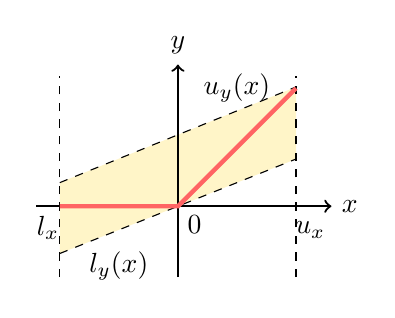
\begin{tikzpicture}[scale=1.5]
            \def\lx{-1.0} \def\ux{1.0} \def\d{0.5}
            \coordinate (A) at (\lx, \d*\lx+0.1);
            \coordinate (B) at (\lx, 0.2);
            \coordinate (E) at (\ux, \ux+0.01);
            \coordinate (F) at (\ux, \ux-\d*\ux-0.1);
            \fill[yellowfill] (A) -- (B) -- (E) -- (F) -- cycle;
            \draw[thick,->] ({\lx-0.2},0) -- ({\ux+0.3},0) node[right] {$x$};
            \draw[thick,->] (0,-0.6) -- (0,{\ux+0.2}) node[above] {$y$};
            \draw[dashed] (\lx,-0.6) -- (\lx,{\ux+0.1});
            \draw[dashed] (\ux,-0.6) -- (\ux,{\ux+0.1});
            \draw[dashed] (\lx, 0.2) -- (\ux, \ux+0.01);
            \draw[dashed] (\lx, \d*\lx+0.1) -- (\ux, \ux-\d*\ux-0.1);
            \draw[ultra thick,myred] (\lx,0) -- (0,0) -- (\ux,\ux);
            \node[below] at (\lx-0.1,0) {$l_x$};
            \node[below] at (\ux+0.12,-0.05) {$u_x$};
            \node[below] at ({\lx/2},-0.3) {$l_{y}(x)$};
            \node[above] at (\ux/2,\ux/2+0.3) {$u_{y}(x)$};
            \node[below right] at (0,0) {$0$};
        \end{tikzpicture}
        \caption{Zonotope}
        \label{fig:relu-zonotope-abstraction}
    \end{subfigure}
    \hfill
    % Second row
    \begin{subfigure}{0.3\linewidth}
        \centering
        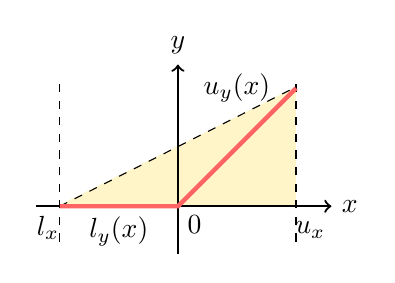
\begin{tikzpicture}[scale=1.5]
            \def\lx{-1.0} \def\ux{1.0} \def\d{0.5}
            \coordinate (A) at (\lx, 0);
            \coordinate (B) at (\lx, 0.01);
            \coordinate (E) at (\ux, \ux+0.01);
            \coordinate (F) at (\ux, 0);
            \fill[yellowfill] (A) -- (B) -- (E) -- (F) -- cycle;
            \draw[thick,->] ({\lx-0.2},0) -- ({\ux+0.3},0) node[right] {$x$};
            \draw[thick,->] (0,-0.4) -- (0,{\ux+0.2}) node[above] {$y$};
            \draw[dashed] (\lx,-0.3) -- (\lx,{\ux+0.1});
            \draw[dashed] (\ux,-0.3) -- (\ux,{\ux+0.1});
            \draw[dashed] (\lx, 0) -- (\ux, \ux+0.01);
            \draw[dashed] (\lx, 0) -- (\ux, 0);
            \draw[ultra thick,myred] (\lx,0) -- (0,0) -- (\ux,\ux);
            \node[below] at (\lx-0.1,0) {$l_x$};
            \node[below] at (\ux+0.12,-0.05) {$u_x$};
            \node[below] at ({\lx/2},-0.01) {$l_{y}(x)$};
            \node[above] at (\ux/2,\ux/2+0.3) {$u_{y}(x)$};
            \node[below right] at (0,0) {$0$};
        \end{tikzpicture}
        \caption{Polytope (lower flat)}
        \label{fig:relu-polytope-abstraction}
    \end{subfigure}

    \caption{Abstractions of $\text{ReLU}(x) = \max(0,x)$ over $x \in [l_x, u_x]$: (a) interval, (b) zonotope, (c–d) polytope abstractions with different lower bounds.}
    \label{fig:relu-all-abstractions}
\end{figure}

\subsection{Common Abstractions for ReLU}
\autoref{fig:relu-all-abstractions} illustrates common abstractions (or \emph{over-approximations}) for the ReLU function $y = \max(0, x)$, where $x \in [l_x, u_x]$ and $y \in [l_y(x), u_y(x)]$. The values of ReLU are shown as points on the \colorbox{myred}{red line}, which is non-convex and consists of two linear segments: one for $x < 0$ (where $y = 0$) and another for $x \geq 0$ (where $y = x$).
To compute the bounds $l_y(x)$ and $u_y(x)$, we can use different abstractions: 

\begin{itemize}
    \item \textbf{Interval Abstraction:} Interval represents the output of the post-ReLU neuron as intervals $[l_y(x), u_y(x)]$ where $l_y(x) = 0$ and $u_y(x) = u_x$. It does not capture the relationship between the input and output of ReLU, and simply assumes that the output can take any value between 0 and the upper bound of the input. Interval is a simple and efficient abstraction, but it can be \emph{too imprecise} for many cases.

    In~\autoref{fig:relu-interval-abstraction}, the \colorbox{yellowfill}{yellow rectangle} represents the interval $[0, u_x]$.  As can be seen, this interval region is too large of an over-approximation (too coarse or loose), as it includes many points that are not achievable by ReLU, e.g., the point $(0.5, 0.0)$ is not on the red line.

    \item \textbf{Zonotope Abstraction:} Zonotopes can capture linear relationships between variables more effectively. We can represent ReLU as a zonotope that includes the linear segments. In \autoref{fig:relu-zonotope-abstraction}, the zonotope is shown as a parallelogram that captures the linear relationship between $x$ and $y$. The lower bound $l_y(x)$ is $y = \lambda x$ and the upper bound $u_y(x)$ is $y = \lambda x + u_x(1 - \lambda)$ for some slope $\lambda \in [0, \frac{u_x}{u_x - l_x}]$. If we set $\lambda = 0$, the zonotope is a rectangle, which is the same as the interval abstraction. If we set $\lambda = \frac{u_x}{u_x - l_x}$, the zonotope's is upper bound is the same as polytope's upper bound in \autoref{fig:relu-polytope-abstraction}.

    The \colorbox{yellowfill}{zonotope} shown in \autoref{fig:relu-zonotope-abstraction} is arguably tighter than the interval abstraction in~\autoref{fig:relu-interval-abstraction}.  It captures the linear relationship between $x$ and $y$ and excludes points that are not achievable by ReLU, e.g., the point $(0.5, 0.0)$ that was included in the interval abstraction is not included in the zonotope. However, it still includes non-ReLU points and is also not strictly better than interval, e.g., the point $(0.5, -0.5)$ is included in the zonotope but not in the interval abstraction (or ReLU).

    \item \textbf{Polytope Abstraction:} Polytopes can represent arbitrary linear constraints and provide very precise bounds. We can construct a polytope that tightly encloses the non-convex shape of the ReLU function.

    In \autoref{fig:relu-polytope-abstraction}, the polytope is shown as a trapezoid that captures the linear segments of ReLU. The lower bound is $l_y(x) = 0$ and the upper bound is $u_y(x) = u_x$. \tvn{this is similar to the interval abstraction, as both have the same bounds, right?}\hd{you mean the same lower bound equation? Yes. Upper bound equation is different. However given a single neuron abstraction like in those figures, the concrete bounds (not the equations) are the same.}

\end{itemize}

% \begin{figure}[h]
%     \centering
    
%     \begin{tikzpicture}[scale=2]
%         % Colors
%         \definecolor{myred}{RGB}{255,100,100}
%         \definecolor{yellowfill}{RGB}{255,245,200}
%         % Parameters
%         \def\lx{-1.0}
%         \def\ux{1.0}
%         \def\ly{0}
%         \def\uy{1.0}
%         % Fill region
%         \fill[yellowfill] (\lx,\ly) rectangle (\ux,\uy);
%         % Axes
%         \draw[thick,->] ({\lx-0.2},0) -- ({\ux+0.3},0) node[right] {$x$};
%         \draw[thick,->] (0,{\ly-0.3}) -- (0,{\uy+0.3}) node[above] {$y$};
%         % Dashed bounds
%         \draw[dashed] (\lx,{\ly-0.1}) -- (\lx,{\uy+0.2});
%         \draw[dashed] (\ux,{\ly-0.1}) -- (\ux,{\uy+0.2});
%         \draw[dashed] (\lx,\uy) -- (\ux,\uy);
%         % ReLU line
%         \draw[ultra thick,myred] (\lx,\ly) -- (0,\ly) -- (\ux,\uy);
%         % Labels
%         \node[below] at (\lx,0) {$l_x$};
%         \node[below] at (\ux,-0.05) {$u_x$};
%         \node[left] at (-0.1,\ly-0.2) {$l_y(x)$};
%         \node[above] at (\ux-0.5,\uy) {$u_y(x)$};
%         % Origin
%         \node[below right] at (0,0) {$0$};
%     \end{tikzpicture}
%     \caption{Interval abstraction for ReLU: $y = \max(0, x)$, with $x \in [l_x, u_x]$ and $y \in [l_y(x), u_y(x)]$.}
%     \label{fig:relu-interval-abstraction}
% \end{figure}

\begin{figure}[h]
    \centering
    \begin{subfigure}{0.49\linewidth}
    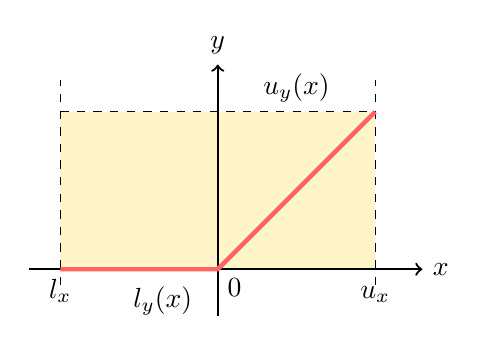
\begin{tikzpicture}[scale=2]
        % Colors
        \definecolor{myred}{RGB}{255,100,100}
        \definecolor{yellowfill}{RGB}{255,245,200}
        % Parameters
        \def\lx{-1.0}
        \def\ux{1.0}
        \def\ly{0}
        \def\uy{1.0}
        % Fill region
        \fill[yellowfill] (\lx,\ly) rectangle (\ux,\uy);
        % Axes
        \draw[thick,->] ({\lx-0.2},0) -- ({\ux+0.3},0) node[right] {$x$};
        \draw[thick,->] (0,{\ly-0.3}) -- (0,{\uy+0.3}) node[above] {$y$};
        % Dashed bounds
        \draw[dashed] (\lx,{\ly-0.1}) -- (\lx,{\uy+0.2});
        \draw[dashed] (\ux,{\ly-0.1}) -- (\ux,{\uy+0.2});
        \draw[dashed] (\lx,\uy) -- (\ux,\uy);
        % ReLU line
        \draw[ultra thick,myred] (\lx,\ly) -- (0,\ly) -- (\ux,\uy);
        % Labels
        \node[below] at (\lx,0) {$l_x$};
        \node[below] at (\ux,-0.05) {$u_x$};
        \node[left] at (-0.1,\ly-0.2) {$l_y(x)$};
        \node[above] at (\ux-0.5,\uy) {$u_y(x)$};
        % Origin
        \node[below right] at (0,0) {$0$};
    \end{tikzpicture}
    \end{subfigure}
    \hfill
    \begin{subfigure}{0.49\linewidth}
        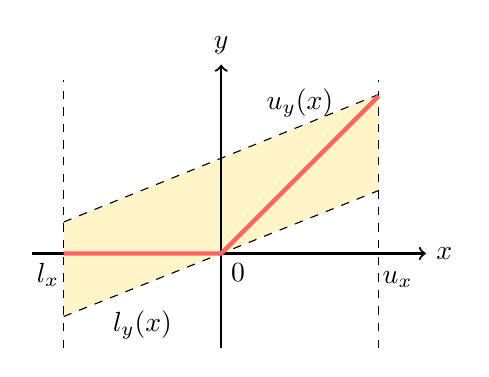
\begin{tikzpicture}[scale=2]
            % Colors
            \definecolor{myred}{RGB}{255,100,100}
            \definecolor{yellowfill}{RGB}{255,245,200}
            % Parameters
            \def\lx{-1.0}
            \def\ux{1.0}
            % Zonotope (band width)
            \def\d{0.5}
            % Zonotope corners
            \coordinate (A) at (\lx, 0+\d*\lx+0.1);    % bottom left
            \coordinate (B) at (\lx, 0.2);    % top left
            \coordinate (C) at (0, \d*0);          % top middle
            \coordinate (D) at (0, -\d*0);         % bottom middle
            \coordinate (E) at (\ux, \ux+0.01);  % top right
            \coordinate (F) at (\ux, \ux-\d*\ux-0.1);  % bottom right
            % Fill zonotope
            \fill[yellowfill] (A) -- (B) -- (E) -- (F) -- cycle;
            % Axes
            \draw[thick,->] ({\lx-0.2},0) -- ({\ux+0.3},0) node[right] {$x$};
            \draw[thick,->] (0,{-0.6}) -- (0,{\ux+0.2}) node[above] {$y$};
            % Bounded region
            \draw[dashed] (\lx,{-0.6}) -- (\lx,{\ux+0.1});
            \draw[dashed] (\ux,{-0.6}) -- (\ux,{\ux+0.1});
            % Zonotope boundaries
            \draw[dashed] (\lx, 0.2) -- (\ux, \ux+0.01);
            \draw[dashed] (\lx, \d*\lx+0.1) -- (\ux, \ux-\d*\ux-0.1);
            % ReLU line
            \draw[ultra thick,myred] (\lx,0) -- (0,0) -- (\ux,\ux);
            % Labels
            \node[below] at (\lx-0.1,0) {$l_x$};
            \node[below] at (\ux+0.12,-0.05) {$u_x$};
            \node[below] at ({\lx/2},-0.3) {$l_{y}(x)$};
            \node[above] at (\ux/2,\ux/2+0.3) {$u_{y}(x)$};
            % Origin
            \node[below right] at (0,0) {$0$};
        \end{tikzpicture}
    \end{subfigure}

    \caption{Zonotope abstraction for ReLU: $y = \max(0,x)$, with $x \in [l_x, u_x]$ and $y \in [l_y(x), u_y(x)]$.}
    \label{fig:relu-zonotope-abstraction2}
\end{figure}


\begin{figure}[h]
    \centering
    \begin{subfigure}{0.49\linewidth}
        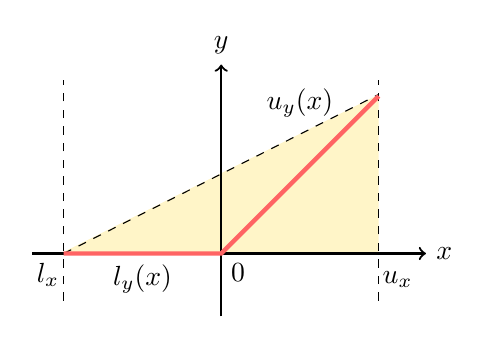
\begin{tikzpicture}[scale=2]
            % Colors
            \definecolor{myred}{RGB}{255,100,100}
            \definecolor{yellowfill}{RGB}{255,245,200}
            % Parameters
            \def\lx{-1.0}
            \def\ux{1.0}
            % Zonotope (band width)
            \def\d{0.5}
            % Zonotope corners
            \coordinate (A) at (\lx, 0);    % bottom left
            \coordinate (B) at (\lx, 0.01);    % top left
            \coordinate (C) at (0, \d*0);          % top middle
            \coordinate (D) at (0, -\d*0);         % bottom middle
            \coordinate (E) at (\ux, \ux+0.01);  % top right
            \coordinate (F) at (\ux, 0);  % bottom right
            % Fill zonotope
            \fill[yellowfill] (A) -- (B) -- (E) -- (F) -- cycle;
            % Axes
            \draw[thick,->] ({\lx-0.2},0) -- ({\ux+0.3},0) node[right] {$x$};
            \draw[thick,->] (0,{-0.4}) -- (0,{\ux+0.2}) node[above] {$y$};
            % Bounded region
            \draw[dashed] (\lx,{-0.3}) -- (\lx,{\ux+0.1});
            \draw[dashed] (\ux,{-0.3}) -- (\ux,{\ux+0.1});
            % Zonotope boundaries
            \draw[dashed] (\lx, 0) -- (\ux, \ux+0.01);
            \draw[dashed] (\lx, 0) -- (\ux, 0);
            % ReLU line
            \draw[ultra thick,myred] (\lx,0) -- (0,0) -- (\ux,\ux);
            % Labels
            \node[below] at (\lx-0.1,0) {$l_x$};
            \node[below] at (\ux+0.12,-0.05) {$u_x$};
            \node[below] at ({\lx/2},-0.01) {$l_{y}(x)$};
            \node[above] at (\ux/2,\ux/2+0.3) {$u_{y}(x)$};
            % Origin
            \node[below right] at (0,0) {$0$};
        \end{tikzpicture}
    \end{subfigure}
    \hfill
    \begin{subfigure}{0.49\linewidth}
        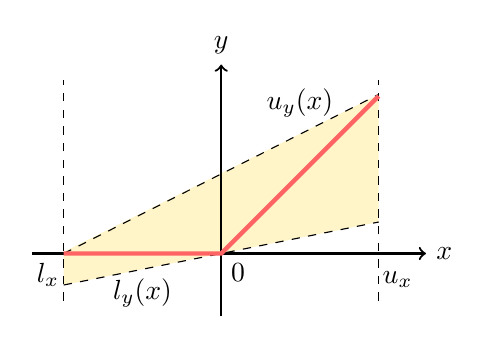
\begin{tikzpicture}[scale=2]
            % Colors
            \definecolor{myred}{RGB}{255,100,100}
            \definecolor{yellowfill}{RGB}{255,245,200}
            % Parameters
            \def\lx{-1.0}
            \def\ux{1.0}
            % Zonotope (band width)
            \def\d{0.5}
            % Zonotope corners
            \coordinate (A) at (\lx, -0.2);    % bottom left
            \coordinate (B) at (\lx, 0.01);    % top left
            \coordinate (C) at (0, \d*0);          % top middle
            \coordinate (D) at (0, -\d*0);         % bottom middle
            \coordinate (E) at (\ux, \ux+0.01);  % top right
            \coordinate (F) at (\ux, 0.2);  % bottom right
            % Fill zonotope
            \fill[yellowfill] (A) -- (B) -- (E) -- (F) -- cycle;
            % Axes
            \draw[thick,->] ({\lx-0.2},0) -- ({\ux+0.3},0) node[right] {$x$};
            \draw[thick,->] (0,{-0.4}) -- (0,{\ux+0.2}) node[above] {$y$};
            % Bounded region
            \draw[dashed] (\lx,{-0.3}) -- (\lx,{\ux+0.1});
            \draw[dashed] (\ux,{-0.3}) -- (\ux,{\ux+0.1});
            % Zonotope boundaries
            \draw[dashed] (\lx, 0) -- (\ux, \ux+0.01);
            \draw[dashed] (\lx, -0.2) -- (\ux, 0.2);
            % ReLU line
            \draw[ultra thick,myred] (\lx,0) -- (0,0) -- (\ux,\ux);
            % Labels
            \node[below] at (\lx-0.1,0) {$l_x$};
            \node[below] at (\ux+0.12,-0.05) {$u_x$};
            \node[below] at ({\lx/2},-0.1) {$l_{y}(x)$};
            \node[above] at (\ux/2,\ux/2+0.3) {$u_{y}(x)$};
            % Origin
            \node[below right] at (0,0) {$0$};
        \end{tikzpicture}
    \end{subfigure}

    \caption{Polytop abstraction for ReLU: $y = \max(0,x)$, with $x \in [l_x, u_x]$ and $y \in [l_y(x), u_y(x)]$.}
    \label{fig:relu-polytope-abstraction2}
\end{figure}


\tvn{Hai, create concrete examples with numbers to show how the abstractions work, e.g., for interval, zonotope, polytope, etc. We want to use one example to show the differences in the approximation,  not multiple examples which would be less effective.}


\subsection{Transformer Functions}

The concept of computing abstractions, often referred to as \emph{abstract interpretation}, is central to program analysis. 
It allows us reason about the behavior of a program without evaluating it on all concrete inputs---which may be infinite. Instead, we use an \emph{abstract domain}, such as interval, to summarize sets of concrete values, enabling sound and scalable approximation.


\paragraph{Abstraction Functions} In abstraction interpretation, we have the \emph{abstraction function}
\[
\alpha : D \to D^a,
\]
which maps a concrete value from the domain $D$ to an element in a finite or simpler abstract domain $D^a$. 

\begin{example}[Odd/Even]
    The \texttt{odd/even} or parity abstraction is defined as:
\[
\alpha_{\texttt{parity}}(x \in \mathbb{Z}) =
\begin{cases}
\texttt{even} & \text{if } x \bmod 2 = 0 \\
\texttt{odd}  & \text{if } x \bmod 2 = 1
\end{cases}
\]
Even though $\mathbb{Z}$ is infinite, this abstraction maps all integers to a finite set $\{\texttt{odd}, \texttt{even}\}$. The abstraction functions $\alpha$ allow us to represent infinite sets compactly.
\end{example}

\paragraph{Transformer Functions} Once we have values in the abstract domains, we often define an \emph{abstract transformer function} 
\[
f^a : D^a \to D^a,
\]
for each operation \(f\) to reason about the effects of \(f\) on abstract values.


\begin{example}[Intervals]
Let $f(x) = x + 1$ and consider the interval abstraction $D^a = \{ [a, b] \mid a \leq b \in \mathbb{Z} \cup \{-\infty, +\infty\} \}$. Then:
\[
f^a([a, b]) = [a+1, b+1]
\]
\end{example}

\begin{example}[Sign abstraction]
Let the abstract domain be $\{\texttt{neg}, \texttt{zero}, \texttt{pos}\}$. For $f(x) = x + 1$, the abstract transformer is:
\[
f^a(\texttt{neg}) = \{\texttt{neg}, \texttt{zero}\}, \quad
f^a(\texttt{zero}) = \texttt{pos}, \quad
f^a(\texttt{pos}) = \texttt{pos}
\]
\end{example}


\section{Abstract Domains and Transformer Functions DNNs}

\subsection{Interval}\label{sec:interval-abstraction}

Interval is a widely-used abstraction technique in DNN verification due to its simplicity and efficiency. It estimates the over-approximated range of values that a neuron can take using a lower and upper bound $[l, u]$, e.g., an interval over the set of values $\{-2.5, -8.2, -10.7, 2, 4.7, 5.1\}$ can be represented as $[-10.7, 5.1]$.

\subsubsection{Abstract Transformers}

We now define abstract transformers for the interval domains for the affine function and ReLU activation.

\paragraph{Affine Function} For the affine function \(f\) in~\autoref{sec:affine}
\[f(v_1, v_2, ...,v_n) = \sum_{i=1}^{n} w_i v_i + b\]
where $n$ is number of output nodes from the previous layer and \(b\) is the bias term. We define the abstract transformer \(f^a\) for interval as:
\[
f^{a}([l_1, u_1],..., [l_n, u_n])
= \Bigg[\sum_{i=1}^{n}\big(w_i^{+} l_i + w_i^{-} u_i\big) + b,\; \sum_{i=1}^{n}\big(w_i^{+} u_i + w_i^{-} l_i\big) + b\Bigg].
\]
where \(w_i^{+} = \max(w_i, 0),\quad w_i^{-} = \min(w_i, 0)\).
% Equivalently, for a vector form \(f(x)=Wx+b\) with entrywise decompositions \(W^{+}=\max(W,0)\) and \(W^{-}=\min(W,0)\), we have
% \[f^a([l,u]) = [\,W^{+}l + W^{-}u + b,\; W^{+}u + W^{-}l + b\,].\]

% Here, \(l \in \mathbb{R}^n\) and \(u \in \mathbb{R}^n\) represent the lower \([l_1,\dots,l_n]\) and upper \([u_1,\dots,u_n]\) bounds of the inputs, respectively.

\begin{example}
Consider \(f^a(x_1,x_2) = -0.5\,x_1 + 0.5\,x_2 + 1.0\) in~\autoref{sec:affine} with
\[x_1 \in [1,2],\quad x_2 \in [-1,3].\]
Here, \(w_1=-0.5\Rightarrow w_1^{+}=0,\; w_1^{-}=-0.5\) and \(w_2=0.5\Rightarrow w_2^{+}=0.5,\; w_2^{-}=0\). Applying the rule,
\[\begin{aligned}
f^a_L &= w_1^{+} l_1 + w_1^{-} u_1 + w_2^{+} l_2 + w_2^{-} u_2 + b \\
    &= 0\cdot 1 + (-0.5)\cdot 2 + 0.5\cdot(-1) + 0\cdot 3 + 1.0 = -0.5,\\
f^a_U &= w_1^{+} u_1 + w_1^{-} l_1 + w_2^{+} u_2 + w_2^{-} l_2 + b \\
    &= 0\cdot 2 + (-0.5)\cdot 1 + 0.5\cdot 3 + 0\cdot(-1) + 1.0 = 2.0.
\end{aligned}\]
Thus, \(f^a([1,2],[-1,3]) = [-0.5,\, 2.0].\)
\end{example}

\subsection{Activation Functions}

Most activation functions (\autoref{sec:activation}) used in neural networks are monotonically increasing, e.g., ReLU and Sigmoid. For interval domain, it is straightforward to define an abstract transformer for any monotonically increasing function \(f : \mathbb{R} \to \mathbb{R}\), as we simply apply \(f\) for lower and upper bounds as follows:
\[f^a
([l, u]) = [ f(l), f(u)]
\]


\begin{example} 
% For the DNN in \autoref{fig:dnn}, the interval abstraction for the input layer is $x_1 \in [-1, 1]$ and $x_2 \in [-2, 2]$. The interval abstraction for the hidden layer is $x_3 \in [0, 2]$ because $x_3 = [ReLU(-0.5x_1 + 0.5x_2 + 1.0), ReLU(-0.5x_1 + 0.5x_2 + 1.0)] = [ReLU(-0.5 \times -1 + 0.5 \times -2 + 1.0), ReLU(-0.5 \times 1 + 0.5 \times 2 + 1.0)] = [0, 2]$. Similarly, $x_4 \in [0, 2]$. The interval abstraction for the output layer is $x_5 \in [-3, 3]$.


\begin{figure}[h]
    \centering
    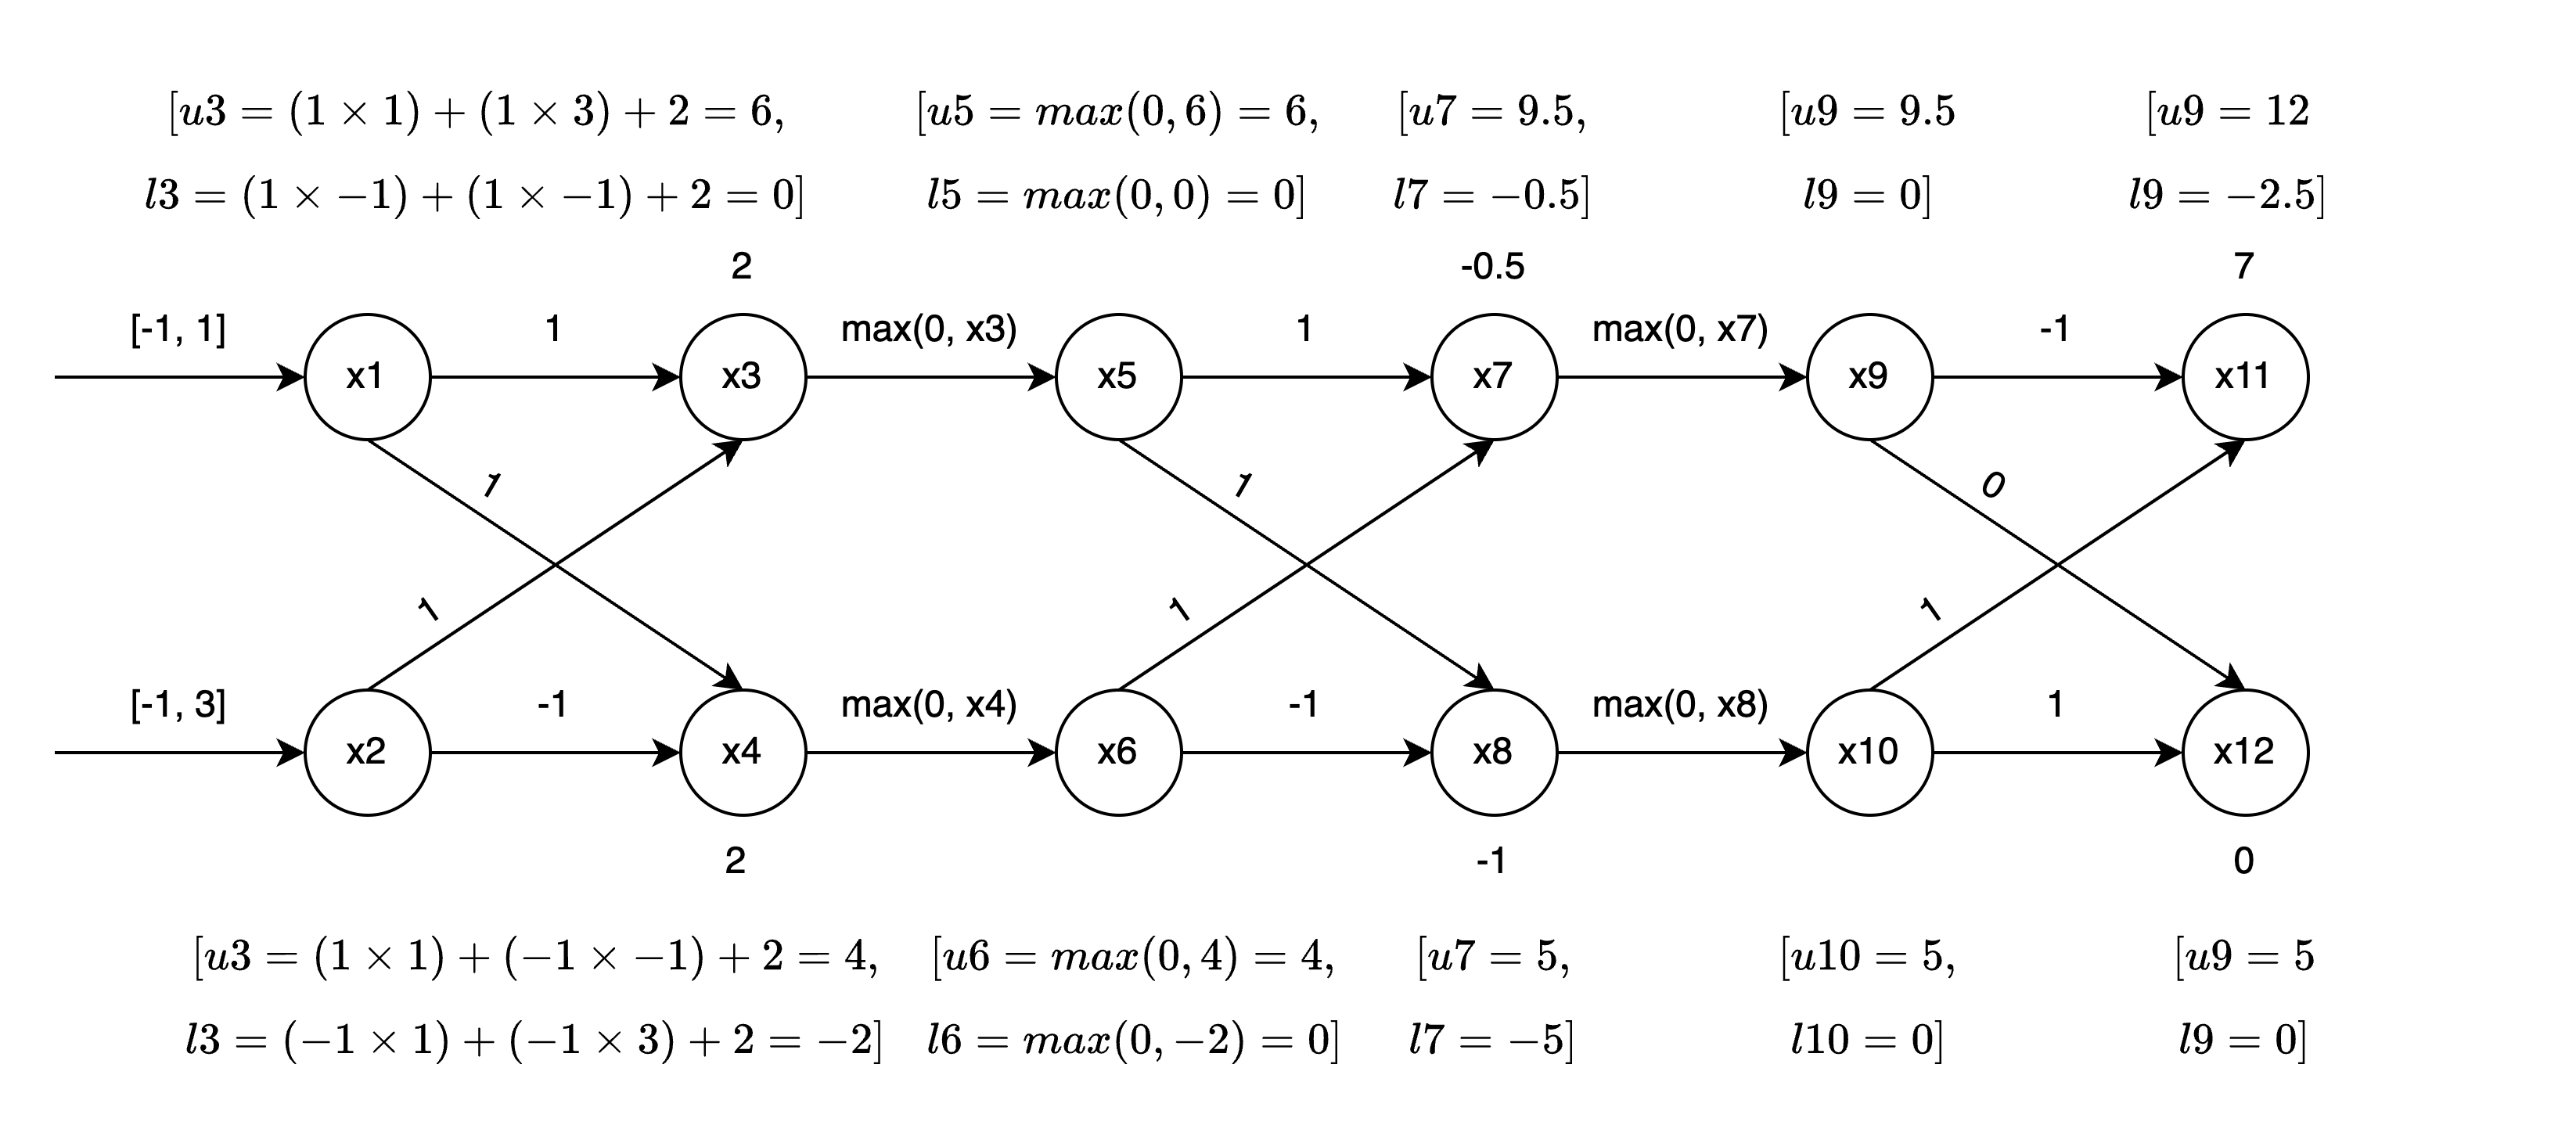
\includegraphics[width=1.2\linewidth]{figure/2_layers_example.png}
    \caption{Feed-forward neural network with 6 layers and 2 neurons per layer.}
    \label{fig:interval-network}
\end{figure}
In~\autoref{fig:interval-network}, we aim to verify whether \(x_{11}\ \geq\ x_{12}\) given a bounded input range on \(x_1\) and \(x_2\). To do this using interval abstraction, we propagate intervals layer by layer.

Suppose the inputs \(x_1\) and \(x_2\) satisfy:
\[
x_1 \in [-1, 1], \quad x_2 \in [-1, 2]
\]

Let an affine neuron (e.g., \(x_3\)) compute:
\[
x_3 = 1 x_1 + 1 x_2 + 2
\]

Then we apply the affine abstract transformer:
<<<<<<< HEAD
\begin{equation}
\begin{aligned}
  x_3 \in & ~[\min(1\times-1, 1\times1) + \min(1\times-1, 1\times3) + 2, \\
          & ~\max(1\times-1, 1\times-1) + \max(-1\times-1, -1\times3) + 2] = \\
          & [0,6]
\end{aligned}         
\end{equation}
=======
\[
\begin{aligned}
x_3 &\in [\,1\cdot l_{x_1} + 1\cdot l_{x_2} + 2,\; 1\cdot u_{x_1} + 1\cdot u_{x_2} + 2\,] \\
    &= [\,(-1)+(-1)+2,\; 1+2+2\,] = [0,\,5].
\end{aligned}
\]
>>>>>>> 391dcbf (updates)

So we over-approximate \(x_3\) as:
\[
x_3 \in [0, 6]
\]

This process is repeated for each layer until we reach the output layer.
Here we can see that by using Interval abstraction, the property \(x_{11}\ \geq\ x_{12}\) or  \(x_{11}\ - x_{12} \geq 0\) is \textit{UNSAT} due to
\[
-2.5 - 0  \leq x_{11}\ -\ x_{12} \leq 12 - 5
\]
\end{example}
\subsection{Zonotope}

Zonotope abstraction is a more precise technique than interval abstraction. Unlike interval abstraction, which considers each variable independently, zonotopes capture correlations between variables (e.g., neuron activations), thereby reducing over-approximation errors.

\subsection{Definition of a Zonotope}

A \textbf{zonotope} is a geometric object that can be viewed as the result of applying an affine transformation to a high-dimensional cube. Formally, a zonotope \(\mathcal{Z}\) in \(\mathbb{R}^n\) is defined as:

\[
\mathcal{Z} = \left\{c + \sum_{i=1}^{m} \epsilon_i g_i \mid \epsilon_i \in [-1, 1]\right\}
\]

where:
\begin{itemize}
    \item \(c \in \mathbb{R}^n\) is the \textit{center} of the zonotope,
    \item \(g_i \in \mathbb{R}^n\) are called \textit{generator vectors},
    \item \(m\) is the number of generators,
    \item \(\epsilon_i\) are independent scalar coefficients bounded between \(-1\) and \(1\).
\end{itemize}

This representation means that the zonotope contains all points that can be formed by adding scaled versions of the generator vectors to the center. The coefficients \(\epsilon_i\) determine the range of influence each generator has.

\paragraph{Example (1D)} Consider a one-dimensional case with \(n = 1\), one generator (\(m = 1\)), and scalar center and generator:

\[
\mathcal{Z} = \left\{c + \epsilon_1 g_1 \mid \epsilon_1 \in [-1, 1]\right\}
\]

This is simply the interval \([c - g_1, c + g_1]\).

\paragraph{Example (2D)} To illustrate zonotopes in higher dimensions, suppose:

\[
c = \begin{bmatrix}2 \\ 3\end{bmatrix}, \quad
g_1 = \begin{bmatrix}1 \\ 1\end{bmatrix}
\]

Then, the set:

\[
\left\{c + \epsilon_1 g_1 \mid \epsilon_1 \in [-1, 1]\right\}
= \left\{
\begin{bmatrix}2 + \epsilon_1 \\ 3 + \epsilon_1\end{bmatrix}
\right\}
\]

describes a line segment \ref{fig:2d1gzonotope-example} between \((1, 2)\) and \((3, 4)\).

\begin{figure}[h]
    \centering
    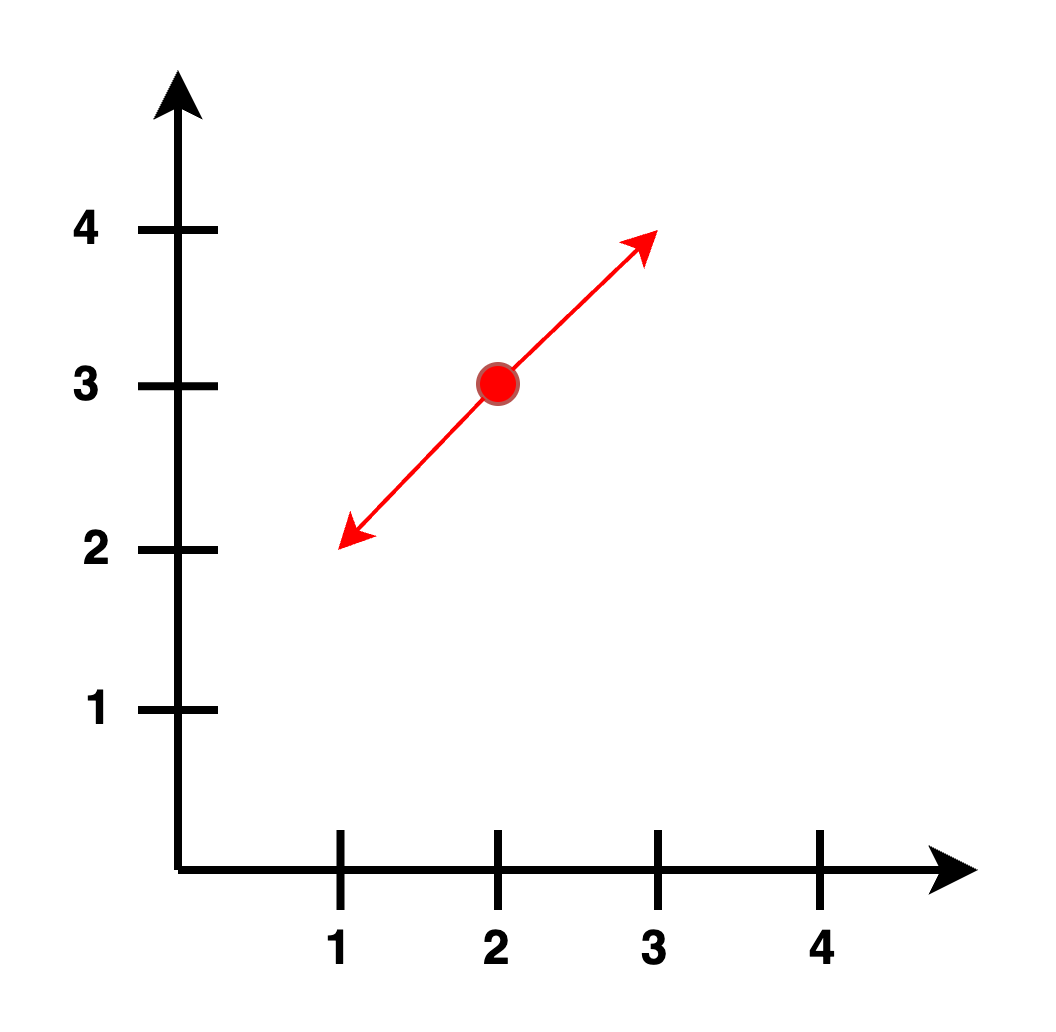
\includegraphics[width=0.5\linewidth]{figure/2d-zonotope.png}
    \caption{Illustration of a 2D zonotope with 1 generator per dimension.}
    \label{fig:2d1gzonotope-example}
\end{figure}

\begin{figure}[h]
    \centering
    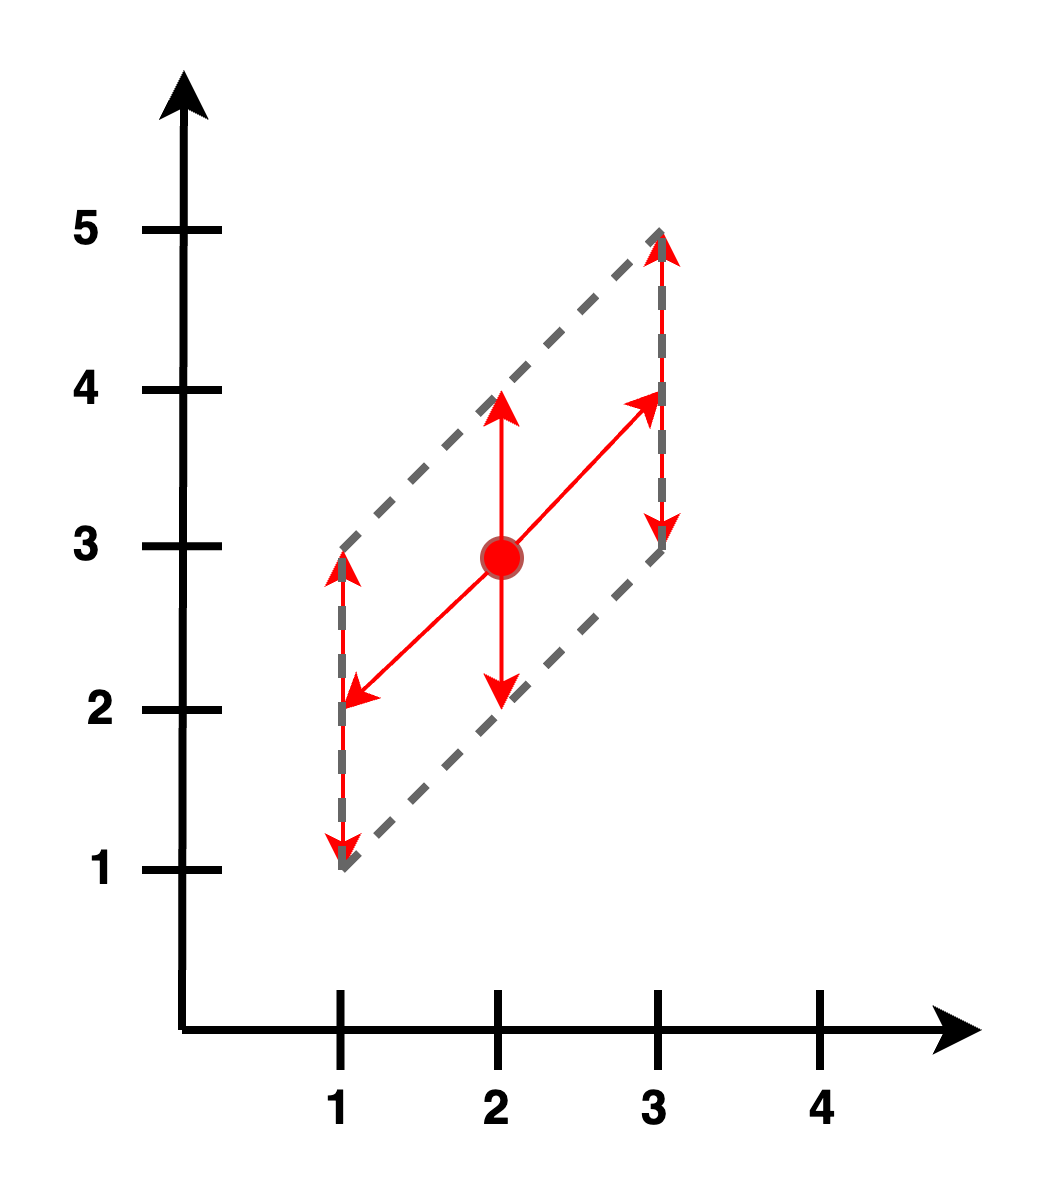
\includegraphics[width=0.5\linewidth]{figure/2-generator-zonotope.png}
    \caption{Illustration of a 2D zonotope with 2 generators per dimension.}
    \label{fig:2d2g-zonotope}
\end{figure}


Now add a second generator:

\[
g_2 = \begin{bmatrix}0 \\ 1\end{bmatrix} 
\]

so it stretches all points along the (0, 1) vector.
The zonotope becomes:

\[
\left\{
\begin{bmatrix}2 \\ 3\end{bmatrix} + \epsilon_1 \begin{bmatrix}1 \\ 1\end{bmatrix} + \epsilon_2 \begin{bmatrix}0 \\ 1\end{bmatrix}
\mid \epsilon_1, \epsilon_2 \in [-1, 1]
\right\}
= \left\{
\begin{bmatrix}2 + \epsilon_1 \\ 3 + \epsilon_1 + \epsilon_2\end{bmatrix}
\right\}
\]


This forms a parallelogram in 2D space \ref{fig:2d2g-zonotope}. As more generators are added, the shape becomes more complex, and the zonotope can approximate more intricate geometric regions.

\subsection{Affine Transformations}

Zonotopes are closed under affine transformations, which makes them especially useful for modeling the linear layers of neural networks.

An affine function is of the form:

\[
f(x) = W x + b
\]

where \(W\) is a weight matrix and \(b\) is a bias vector. Given a zonotope \(\mathcal{Z} = (c, G)\), where \(G\) is a matrix whose columns are the generator vectors \(g_i\), we define the abstract transformer:

\[
f^a(\mathcal{Z}) = (Wc + b, WG)
\]

This means:
\begin{itemize}
    \item The new center is \(Wc + b\) - the weighted sum of input nodes's centers
    \item The new generator matrix is \(WG\) - the weighted sum of input nodes's corresponding generators, where \(W\) is applied to each generator 
\end{itemize}

Since affine functions preserve the zonotope structure, no over-approximation is introduced at this stage.

\subsection{Non-Linear Activation Functions}

Activation functions such as ReLU are not affine and therefore do not preserve the zonotope structure. To handle them, conservative approximations are used.

\paragraph{ReLU Relaxation:} Suppose a neuron has input represented as a zonotope, and we apply the ReLU function \(\text{ReLU}(x) = \max(0, x)\). There are three cases:

\begin{itemize}
    \item \(\mathbf{l_x \geq 0:}\) If all possible values of the neuron (based on the zonotope) are non-negative, ReLU simply returns the values back.
    \item  \(\mathbf{u_x \leq 0:}\): If all possible values of the neuron are negative, the values of the centers and generators are set to 0s.
    \item \textbf{Mixed range:} If the range of values crosses zero, they must be over-approximated. A common method is to introduce new generator vectors like \ref{fig:zonotope_vs_interval} to fit the shape of ReLU more tightly.
\end{itemize}

\begin{figure}
    \centering
    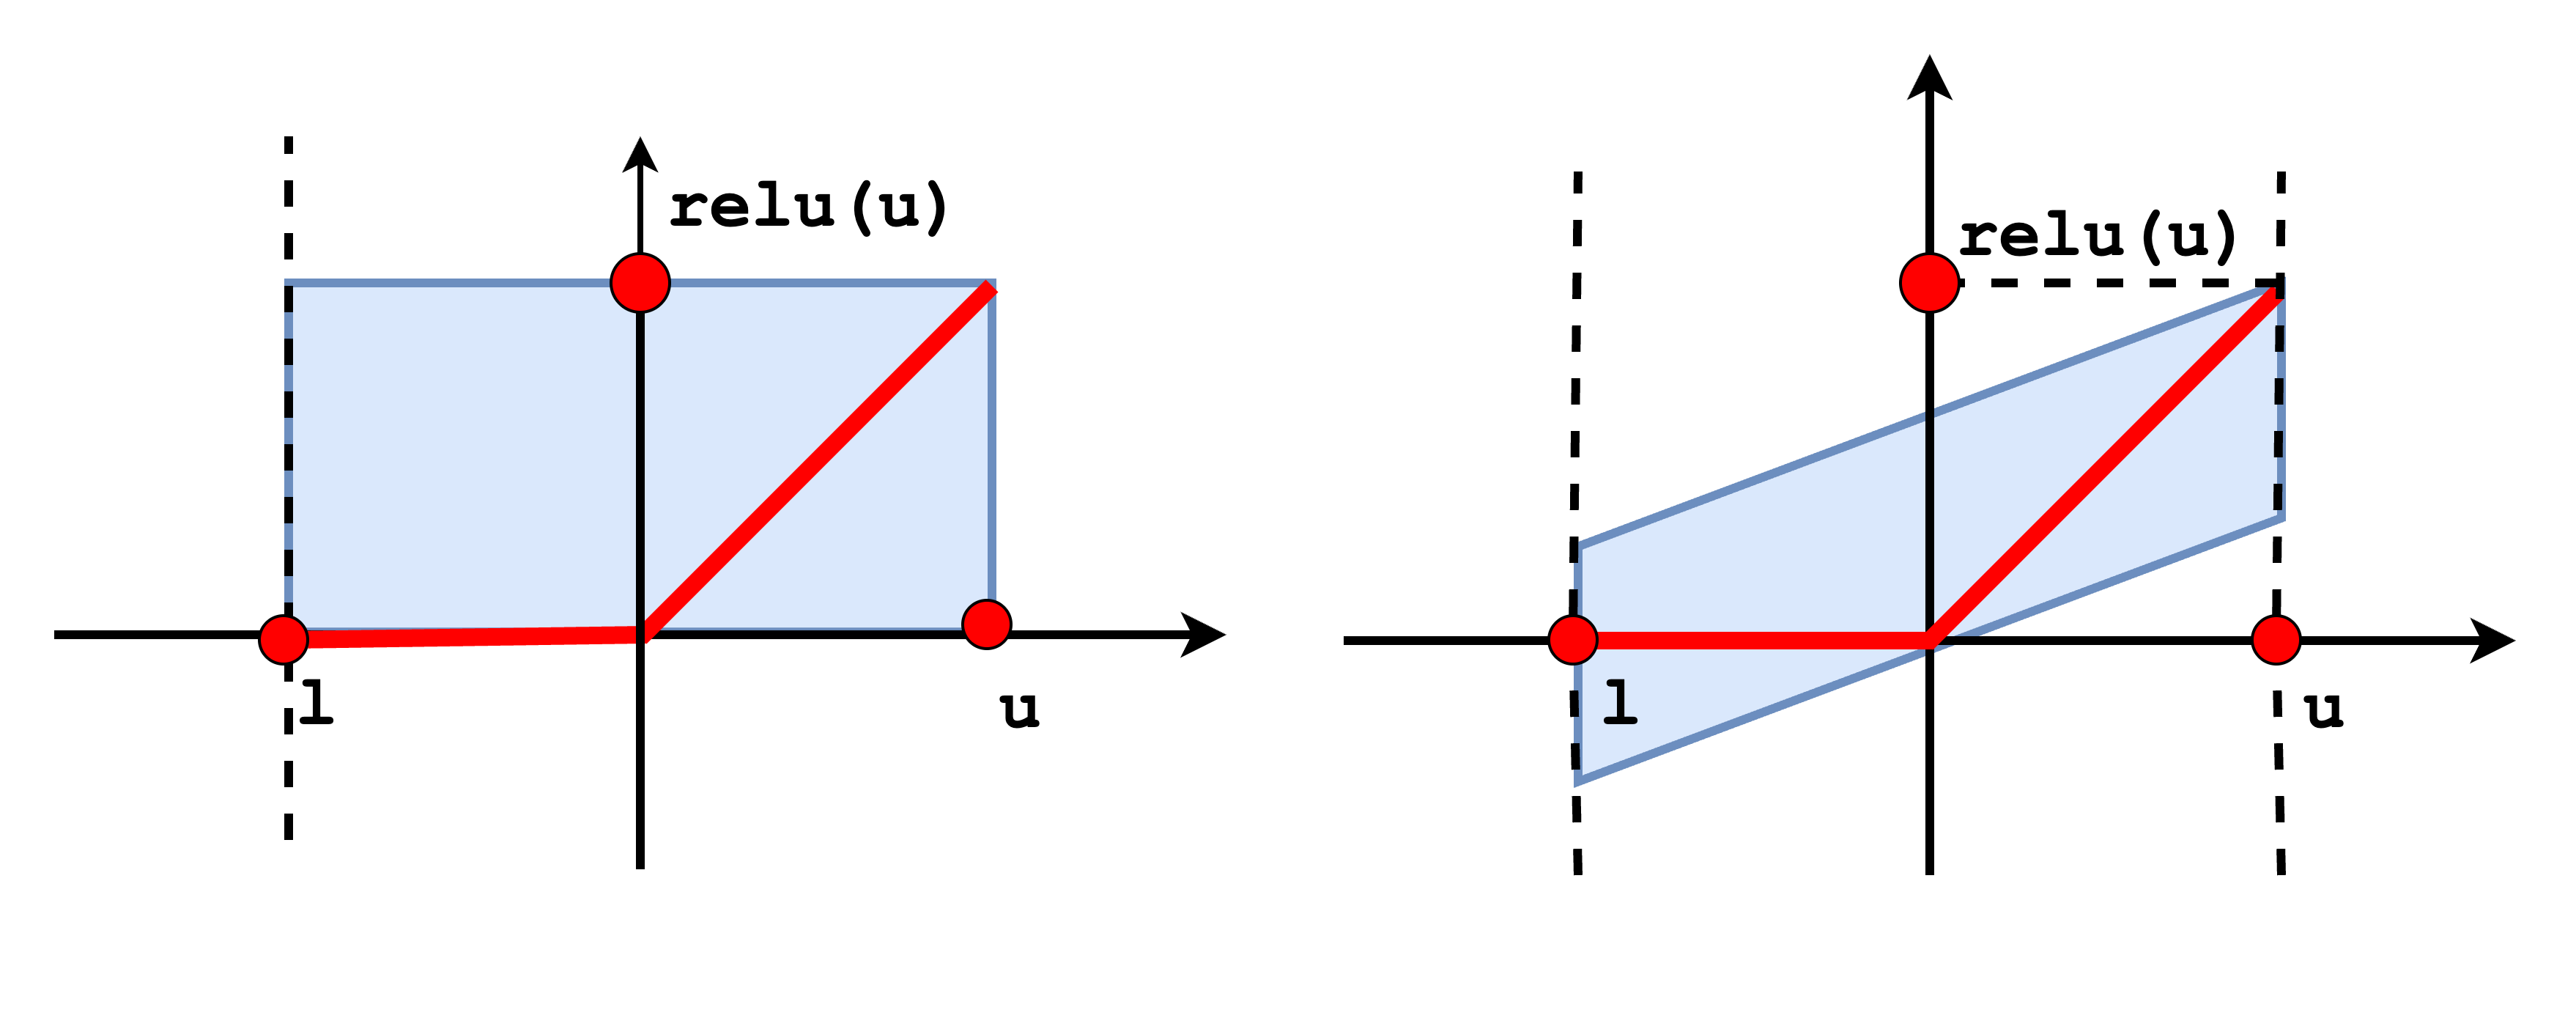
\includegraphics[width=1\linewidth]{figure/zonotope_vs_interval.png}
    \caption{\textbf{Left:} ReLU's Interval approximation. \textbf{Right:} Zonotope approximation counterpart.}
    \label{fig:zonotope_vs_interval}
\end{figure}


The bottom face of the zonotope is the line
\[
y = \lambda x
\]
for some slope \(\lambda\). It follows that the top face must be
\[
y = \lambda x + u(1 - \lambda)
\]

If we set \(\lambda = 0\), we get two horizontal faces, i.e., the interval approximation shown in the left above \ref{fig:zonotope_vs_interval}. The higher we crank up \(\lambda\), the tighter the parallelogram gets. But, we can’t increase \(\lambda\) past \( \frac{u}{u - l} \); this ensures that the parallelogram covers the ReLU along the input range \([l, u]\). So, we will set
\[
\lambda = \frac{u}{u - l}
\]

This relaxation is necessary to ensure soundness (i.e., all real behaviors are contained), but it introduces some loss of precision.

\paragraph{Example:} Let the input zonotope be:

\[
\mathcal{Z}_{\text{input}} = (c, G), \quad
c = \begin{bmatrix} 0 \\ 0 \end{bmatrix}, \quad
G = \begin{bmatrix} 1 & 0 \\ 0 & 2 \end{bmatrix}
\]

This describes the domain:
\[
x_1 \in [-1, 1], \quad x_2 \in [-2, 2]
\]

Now consider the ReLU layer:

\[
x_3 = \text{ReLU}(-0.5x_1 + 0.5x_2 + 1.0)
\]
\[
x_4 = \text{ReLU}(0.5x_1 - 0.5x_2 + 1.0)
\]

First, apply the affine transformation:

\[
\mathcal{Z}_{\text{affine}} = (Wc + b, WG)
\]

Next, check whether each component's range crosses zero. If it does, use ReLU relaxation techniques such as:

\begin{itemize}
    \item \textbf{DeepZ} – introduces extra generators to improve precision,
    \item \textbf{AI\(^2\)} – uses zonotope splitting for tighter bounds.
\end{itemize}

After relaxation, apply the next affine transformation to complete the forward pass.

\subsection{Comparison with Interval Abstraction}

Interval abstraction represents each neuron as an independent interval \([a_i, b_i]\). While simple and fast, it loses inter-variable relationships, leading to large over-approximation errors, especially in deeper networks.

In contrast, zonotopes retain dependencies between neurons via shared generators, providing tighter bounds and better scalability. However, they come at the cost of increased complexity, especially when dealing with non-linear operations.

\paragraph{Summary:}
\begin{itemize}
    \item \textbf{Interval abstraction} is simple but imprecise.
    \item \textbf{Zonotope abstraction} is more precise and scalable, particularly effective for networks with affine layers.
    \item \textbf{Non-linear activations} introduce challenges, requiring trade-offs between precision and computational overhead.
\end{itemize}



\section{Polytope}

In the previous section, we have seen the abstract domain of zonotopes, which is more expressive than the interval domain. Specifically, instead of approximating functions using a hyper-rectangle, the zonotope domain allows us to approximate functions using a zonotope, e.g., a parallelogram, capturing relations between different dimensions. In this section, we look at an even more expressive abstract domain, the polyhedron (or polytope) domain. 

Unlike the zonotope domain, the polyhedron domain allows us to approximate functions using arbitrary convex polyhedra. A polyhedron in \(\mathbb{R}^n\) is a region made of straight (as opposed to curved) faces; a convex shape is one where the line between any two points in the shape is completely contained in the shape. Convex polyhedra can be specified as a set of linear inequalities of the form:

\[
Ax \leq b
\]

where \(A \in \mathbb{R}^{m \times n}\) and \(b \in \mathbb{R}^m\) for some \(m\), specifying \(m\) half-spaces whose intersection forms the polyhedron.

Using a set of convex polyhedra, we can more precisely approximate activation functions like ReLU. For instance, to approximate ReLU, we can describe the tightest convex over-approximation by the following constraints:

\[
x \leq y, \quad 0 \leq y, \quad y \leq \lambda x + \mu
\]

where \(\lambda\) and \(\mu\) are parameters chosen based on the bounds of \(x\).

\begin{figure}[h]
    \centering
    \includegraphics[width=0.5\linewidth]{figure/3-lines-polytope.png}
    \caption{The tightest Convex Polyhedral Approximation of ReLU.}
    \label{fig:enter-label}
\end{figure}
% \begin{figure}
%     \centering
%     \includegraphics[width=0.5\linewidth]{3-lines-polytope.png}
%     \caption{Enter Caption}
%     \label{fig:enter-label}
% \end{figure}

This is the smallest convex polyhedron that soundly approximates ReLU, and is strictly more precise than the interval and zonotope abstractions, as can be seen visually.

\subsection{Affine Functions}

Affine transformations map convex polyhedra to convex polyhedra.  
Given an affine transformation \(f(x) = Wx + b\), where \(W\) is a matrix and \(b\) is a bias vector, we can transform a polyhedron \(\{x \mid A x \leq b\}\) through \(f\) by substitution:

\[
\{x \mid A (W^{-1}(x - b)) \leq b\}
\]

if \(W\) is invertible. More commonly in practice, when applying affine transformations in neural networks (layer-wise), we modify the constraints accordingly by propagating through the weights and biases.

Thus, affine layers can be handled exactly under polyhedral abstraction without any need for relaxation or over-approximation.

\subsection{Activation Functions}

Handling non-linear activation functions, such as ReLU, with polyhedral abstraction is challenging because non-linearities generally map polytopes to non-convex shapes. Therefore, over-approximations are required.

The key idea is to approximate the graph of the non-linear function by a convex polyhedron that covers all possible cases. For ReLU, the previously mentioned three constraints:

\begin{equation}\label{minimum_polyhedron}
x \leq y, \quad 0 \leq y, \quad y \leq \lambda x + \mu
\end{equation}


construct a tight convex relaxation.

For other activations like sigmoid or tanh, the approximation involves linearizing the curve between the lower and upper bounds of the input variable, but the number of constraints can quickly grow, increasing computational complexity.

\paragraph{DeepPoly.}  
By containing two lower polyhedra constraints for \(y\), the approximation in \ref{minimum_polyhedron} inherently suffers from a potential blow-up in number of constraints as the analysis proceeds. Due to scalability issues associated with general polyhedral representations, DeepPoly \cite{singh2019abstract} was proposed as a precise and scalable abstract domain. DeepPoly introduces a specialized form of polyhedral abstraction combined with interval bounds. 

More specifically,  DeepPoly only allows for one lower bound in \ref{minimum_polyhedron}, the selection of which lower constraint depends on which constraint provides the tighter approximation.

Returning to our example, the area of the approximation in Fig.~4(b) is given by \( 0.5 \cdot u \cdot (u - l) \), while the area in Fig.~4(c) is given by \( 0.5 \cdot (-l_i) \cdot (u_i - l_i) \). To achieve a tighter relaxation, we select the approximation with the smaller area. Specifically, when \( u \leq -l \), we apply the constraints and bounds derived from \(x \leq y\).
In addition, each neuron \(x_j\) is bounded above and below by affine expressions of the input neurons:

\[
l_j(x) \leq x_j \leq u_j(x)
\]

where \(l_j\) and \(u_j\) are affine functions.

\subsection{DeepPoly Transformers}

The DeepPoly abstract domain defines a scalable and precise framework for verifying deep neural networks by combining interval and polyhedral abstractions. Each neuron is bounded from above and below using affine expressions of the input neurons:

\[
l_j(x) \leq x_j \leq u_j(x)
\]

where \(l_j(x)\) and \(u_j(x)\) are affine functions representing lower and upper bounds respectively. DeepPoly then defines **abstract transformers** to propagate these bounds through different types of neural network layers.

\subsubsection{Affine Layer Transformer}

Given an affine transformation:
\[
x^{(l+1)} = W x^{(l)} + b
\]

we define the transformation of the bounds by propagating the affine expressions directly:
\begin{align*}
l_j^{(l+1)}(x) &= \sum_i w_{ji}^+ \cdot l_i^{(l)}(x) + w_{ji}^- \cdot u_i^{(l)}(x) + b_j \\
u_j^{(l+1)}(x) &= \sum_i w_{ji}^+ \cdot u_i^{(l)}(x) + w_{ji}^- \cdot l_i^{(l)}(x) + b_j
\end{align*}

Here, \(w^+_{ji} = \max(w_{ji}, 0)\), and \(w^-_{ji} = \min(w_{ji}, 0)\), ensuring correct handling of sign-dependent propagation.

\subsubsection{ReLU Transformer}

The ReLU transformer in DeepPoly uses a convex relaxation that is tighter than previous abstractions by selecting only one lower bound constraint depending on the sign and tightness. Suppose \(x_j = \text{ReLU}(x_i)\). Let \([l_i, u_i]\) be the lower and upper bounds for \(x_i\).

\begin{itemize}
    \item If \(l_i \geq 0\): ReLU is linear, so
    \[
    l_j(x) = l_i(x), \quad u_j(x) = u_i(x)
    \]

    \item If \(u_i \leq 0\): ReLU is constant 0, so
    \[
    l_j(x) = u_j(x) = 0
    \]

    \item If \(l_i < 0 < u_i\): ReLU is approximated with:
    \[
    u_j(x) = \frac{u_i}{u_i - l_i} \cdot (x_i - l_i)
    \]
    and only one lower bound is selected:
    \[
    l_j(x) =
    \begin{cases}
        0, & \text{if area under lower 0 line is smaller} \\
        x_i, & \text{if area under identity line is smaller}
    \end{cases}
    \]
\end{itemize}

The decision is made based on which convex region has smaller area to achieve a tighter abstraction, following the principle:
\[
\text{Choose constraint with smaller area:} \quad 0.5 \cdot u_i \cdot (u_i - l_i) \quad \text{vs} \quad 0.5 \cdot (-l_i) \cdot (u_i - l_i)
\]


By maintaining only upper and lower affine bounds, DeepPoly avoids the full complexity of manipulating arbitrary polytopes while retaining significantly more precision than intervals or zonotopes. 

...

Thus, DeepPoly achieves a practical balance between precision and scalability for verifying deep neural networks.

\subsection{Example}

Consider again the DNN in \autoref{fig:dnn}. Suppose the input set is defined by box constraints \(x_1 \in [-1,1]\) and \(x_2 \in [-2,2]\). These can be represented initially by 4 inequalities.

Applying the affine transformation for the hidden layer, we obtain a new set of inequalities describing the hidden layer nodes. Upon applying ReLU, we would use the convex polyhedral relaxation as depicted in \autoref{fig:3_lines_polytope}. The output layer similarly results from affine operations on the polyhedra describing the hidden layer.

In a DeepPoly setting, instead of carrying full inequalities, we track only the lower and upper affine bounds per neuron, leading to an efficient verification process.

\subsection{Comparison to Zonotope Abstraction}

While zonotope abstraction captures dependencies between variables better than intervals, it still assumes symmetrical dependencies around a center point and cannot easily model arbitrary convex shapes.

Polyhedral abstraction, on the other hand, allows representing arbitrary convex shapes precisely, enabling much tighter approximations, especially after ReLU activations.

However, traditional polyhedral methods suffer from:
\begin{itemize}
    \item High computational complexity,
    \item Rapid growth in the number of constraints,
    \item Difficulty scaling to large networks.
\end{itemize}

DeepPoly addresses these challenges by:
\begin{itemize}
    \item Restricting to simple upper and lower affine bounds,
    \item Maintaining polynomial scalability,
    \item Achieving higher precision than zonotopes or intervals,
    \item Providing efficient transformers for common layers in DNNs.
\end{itemize}

Therefore, DeepPoly achieves a balance, combining the expressiveness of polyhedral domains with the efficiency required for deep network verification.


\section{Abstractions for Other Activation Functions}

\part{DNN Verification Algorithms}
\chapter{The Branch and Bound Search Algorithm}\label{chap:bab}

Modern DNN verifiers typically adopt the Branch-and-Bound (BaB) approach to search for activation patterns (\autoref{sec:activation-pattern}).  At its core, a BaB search consists of two main components: (branch) splitting into the problem smaller subproblems
by using \emph{neuron splitting}, which decides boolean values representing neuron activation status,
and (bound) using abstraction and LP solving to approximate bounds on neuron values to determine
the satisfiability of the partial activation pattern (\autoref{sec:activation-pattern}) formed by the split.

\section{The Algorithm}\label{sec:bab-alg}

\SetKwData{nextlayer}{layer$_{i+1}$}
\SetKwData{status}{status}
\SetKwData{minimum}{objval}

\SetKwFunction{InputMILP}{AddInputConstrs}
\SetKwFunction{GetUnstableNeurons}{GetUnstableNeurons}
\SetKwFunction{PiecewiseLinearMILP}{AddConstrsPWL}
\SetKwFunction{LinearMILP}{AddConstrsLinear}
\SetKwFunction{Maximize}{Maximize}
\SetKwFunction{Minimize}{Minimize}
\SetKwFunction{Feasible}{CheckFeasibility}
\SetKwFunction{Optimize}{Optimize}
\SetKwFunction{isPiecewiseLinear}{isPiecewiseLinear}
\SetKwFunction{CreateStabilizedMILP}{CreateStabilizedMILP}
\SetKwFunction{GetLeafNodes}{GetLeafNodes}
\SetKwFunction{AddConstrs}{AddConstrs}
\SetKwFunction{RemoveConstrs}{RemoveConstrs}
\SetKwFunction{AddObjective}{AddObjectives}
\SetKwFunction{ShortenSplitConstrs}{ShortenSplitConstrs}
\SetKwFunction{RemoveLeafNodes}{RemoveLeaves}
\SetKwFunction{StoppingConditions}{StoppingConditions}
\SetKwFunction{RepOK}{RepOK}
\SetKwFunction{RaiseError}{RaiseError}

\SetKwInOut{Input}{input}
\SetKwInOut{Output}{output}
\SetKw{Break}{break}
\SetKw{Continue}{continue}
\SetKwFunction{Backtrack}{Backtrack}
\SetKwFunction{Select}{Select}
\SetKwFunction{Decide}{Decide}
\SetKwFunction{BCP}{BCP}
\SetKwFunction{Deduce}{Deduce}
\SetKwFunction{AnalyzeConflict}{AnalyzeConflict}
\SetKwFunction{BooleanAbstraction}{BooleanAbstraction}
\SetKwFunction{AddClause}{AddClause}
\SetKwFunction{isTotal}{isTotal}
\SetKwFunction{randomattack}{RandomAttack}
\SetKwFunction{pgd}{PGDAttack}

\SetKwFunction{DPLLT}{DPLLT}
\SetKwFunction{isValid}{isValid}
\SetKwFunction{isEmpty}{isEmpty}
\SetKwFunction{LPSolver}{LPSolver}
\SetKwFunction{Solve}{Solve}
\SetKwFunction{FindLayerNodes}{FindLayerNodes}
\SetKwFunction{TightenInputBounds}{TightenInputBounds}
\SetKwFunction{Abstract}{Abstract}
\SetKwFunction{Check}{Check}
\SetKwFunction{Decide}{Decide}
\SetKwFunction{Imply}{Imply}
\SetKwFunction{Lower}{LowerBound}
\SetKwFunction{Upper}{UpperBound}
\SetKwFunction{GetInputBounds}{GetInputBounds}
\SetKwFunction{GetInputs}{GetInputs}
\SetKwFunction{GetNumInputs}{GetNumInputs}
\SetKwFunction{CurrentConflictClause}{CurrentConflictClause}
\SetKwFunction{StopCriterion}{StopCriterion}
\SetKwFunction{LastAssignedLiteral}{LastLiteral}
\SetKwFunction{LiteralToVariable}{LiteralToVariable}
\SetKwFunction{Antecedent}{Antecedent}
\SetKwFunction{BinRes}{BinRes}
\SetKwFunction{BacktrackLevel}{BacktrackLevel}
\SetKwFunction{AddClause}{AddClause}
\SetKwFunction{ActivationStatus}{ActivationStatus}
\SetKwFunction{Backjump}{Backjump}
\SetKwFunction{EstimateBounds}{EstimateBounds}


\SetKwData{implicationgraph}{igraph}
\SetKwData{literal}{lit}
\SetKwData{variable}{var}
\SetKwData{antecedent}{ante}
\SetKwData{conflict}{conflict}
\SetKwData{none}{none}
\SetKwData{layerid}{lid}
\SetKwData{hiddenbounds}{hidden\_bounds}
\SetKwData{inputs}{inputs}
\SetKwData{inputbounds}{input\_bounds}
\SetKwData{outputbounds}{output\_bounds}
\SetKwData{infeasible}{INFEASIBLE}
\SetKwData{unreachable}{UNREACHABLE}
\SetKwData{maxinputs}{MAX\_NUM\_INPUT}
\SetKwData{assignment}{$\sigma$}
\SetKwData{dl}{dl}
\SetKwData{lpmodel}{solver}
\SetKwData{clauses}{clauses}
\SetKwData{conflict}{conflict}
\SetKwData{clause}{clause}
\SetKwData{igraph}{igraph}
\SetKwData{cex}{cex}
\SetKwData{mysat}{sat}
\SetKwData{myunsat}{unsat}


\SetKwData{submodel}{sub\_model}

\SetKwData{true}{true}
\SetKwData{false}{false}
    
\SetKwFunction{Restart}{Restart}

\SetKwData{counterexample}{cex}
\SetKwData{conflictclause}{conflict\_clause}
\SetKwData{isconflict}{is\_conflict}


\SetKwData{problems}{ActPatterns}
\begin{algorithm}
    \footnotesize
    \Input{DNN $\mathcal{N}$, property $\phi_{in} \Rightarrow \phi_{out}$}
    \Output{$\myunsat$ if property is valid, otherwise ($\mysat, \counterexample$)}
    \BlankLine

    $\problems \leftarrow \{ \emptyset \}$ \tcp{initialize verification problems} 
    % $\prooftree \gets \{ ~ \}$ \tcp{initialize proof tree}\label{line:prooftree}
    
    \While(\tcp*[h]{main loop}){$\problems$}{\label{line:dpllstart}
        % \tcp{$\sigma_i$ is the activation pattern of problem $i$-th}
        $\sigma_i \gets \Select(\problems)$ \tcp{process problem $i$-th}
        % \Parfor(\tcp*[h]{process in parallel}){$\sigma_i ~\In~ \problems$}{ \label{line:parfor}
            \If{\Deduce{$\mathcal{N}, \phi_{in}, \phi_{out}, \sigma_i$}}{\label{line:deduce}
                $(\counterexample, v_i) \leftarrow \Decide(\mathcal{N}, \phi_{in}, \phi_{out}, \sigma_i)$ \\ \label{line:decide}
                \If(\tcp*[h]{found a valid counter-example}){$\counterexample$}{
                    \Return{$(\mysat, \counterexample)$} 
                }
                \tcp{create new activation patterns}
                $\problems \leftarrow \problems \cup \{ \sigma_i \land v_i ~;~ \sigma_i \land \overline{v_i} \}$ \;
            }
            %\Else(\tcp*[h]{detect a conflict}){
                % $\clauses \leftarrow \clauses \cup \AnalyzeConflict(\igraph_i)$ \\ \label{line:analyze_conflict}
            %    $\prooftree \leftarrow \prooftree \cup \{ \sigma_i \}$ \tcp{build proof tree} \label{line:record_proof}
            %}
        % }
        % \If(\tcp*[h]{no more problems}){$\isEmpty(\problems)$}{
        % }
        
    }\label{line:dpllend}
    \Return{\myunsat}
    
    \caption{The \bab{} algorithm.}\label{alg:bab}
\end{algorithm}


\autoref{alg:bab} shows \bab{}, a reference BaB architecture~\cite{nakagawa2014consolidating} for modern DNN verifiers. \bab{} takes as input a ReLU-based DNN $\mathcal{N}$ and a formulae $\phi_{in}\Rightarrow \phi_{out}$ representing the property of interest.
\bab{} maintains a set of activation patterns (\texttt{ActPatterns}) that represent the current activation pattern of the DNN. Initially, \texttt{ActPatterns} is initialized with an empty activation pattern (\autoref{line:activation}).
In each iteration, \bab{} selects an activation pattern $\sigma_i$ from \texttt{ActPatterns} (\tvn{also remove $\sigma_i$ from \texttt{ActPatterns}}?).  It then calls \functiontextformat{Deduce} to check the feasibility of the problem based on the current activation pattern. (Note that we do this even on the empty activation pattern, which is the initial state of the search, because the problem might be trivially infeasible.)

If \functiontextformat{Deduce} determines that the problem is feasible (using the current activation pattern $\sigma_i$), it calls \functiontextformat{Decide} to select a neuron $v_i$ to split, which essentially means the problem is split into two independent subproblems: one with $v_i$ (active) and the other with $\overline{v_i}$ (inactive). \bab{} then adds the two new activation patterns $\sigma_i \land v_i$ and $\sigma_i \land \overline{v_i}$ to \texttt{ActPatterns}. \bab{} then loops back to \autoref{line:dpllstart} to process the next activation pattern.
\tvn{briefly describe what Decide do? in particular what does it do to determine/create an cex when the activation pattern is partially assigned?}


If \functiontextformat{Deduce} determines that the problem is infeasible, it loops back to \autoref{line:dpllstart} to process the next activation pattern. \bab{} terminates when there are no more activation patterns to process, at which point it returns \unsat, indicating that the property is valid.

\tvn{shows that \bab{} often does not exhaust all activation patterns, but rather prunes the search space by deducing infeasibility of some activation patterns.  May be use a tree example to illustrate this?}

%it analyzes the conflict and adds a new clause to the set of clauses (\texttt{clauses}) to prevent the same activation pattern from being selected again.
%The algorithm continues until there are no more activation patterns to process, at which point it returns \unsat, indicating that the property is valid. If a counterexample is found during the search, it returns \sat along with the counterexample. 




%To add proof generation capability, \bab{} is instrumented with a proof tree (\texttt{proof}) variable (\autoref{line:prooftree}) to record these branching decisions. The proof is represented as a binary tree structure, where each node represents a neuron and its left and right edges represent its activation decision (active or inactive). %The proof tree is then used to generate a proof in the \prooflang{} format (\autoref{sec:proof-format}).

\begin{figure}
    \centering
    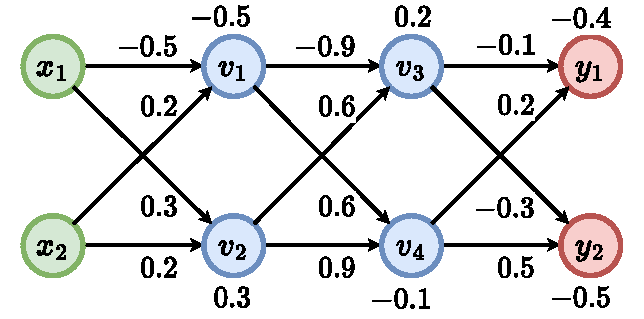
\includegraphics[width=0.5\linewidth]{figure/proof_net.pdf}
    \caption{A simple DNN.}\label{fig:example1}
\end{figure}
%White nodes correspond to branching nodes where \neuralsat{} makes decisions to split ReLU neurons.

\begin{example} 
    
    \tvn{We should change this example to the 5-neuron DNN we have always been using.}\autoref{fig:example1}a illustrates a DNN and how \bab{} verifies that this DNN has the property 
\[
(x_1, x_2) \in [-2.0, 2.0] \times [-1.0, 1,0] \Rightarrow (y_1 > y_2).
\] 

First, \bab{} initializes the activation pattern set \functiontextformat{ActPatterns} with an empty activation pattern $\emptyset$ (\autoref{line:activation}). Then \bab{} enters a loop (\autoref{line:dpllstart}--\autoref{line:dpllend}) to search for a satisfying assignment. In the first iteration, \bab{} selects the only available activation pattern $\emptyset \in \functiontextformat{ActPatterns}$. 
It calls \functiontextformat{Deduce} to check the feasibility of the problem based on the current activation pattern. \functiontextformat{Deduce} uses abstraction to approximate that from the input constraints the output values are feasible for the given network. 
Since \functiontextformat{Deduce} cannot decide infeasibility, \bab{} randomly selects a neuron to split (\functiontextformat{Decide}). Let us assume that it chooses $v_4$ to split, which essentially means the problem is split into two independent subproblems: one with $v_4$ active and the other with $v_4$ inactive.
\bab{} then adds $\{v_4\}$ and $\{\overline{v_4}\}$ to \functiontextformat{ActPatterns}.

In the second iteration, \bab{} has two subproblems (that can be processed in parallel). For the first subproblem with $v_4$, \functiontextformat{Deduce} cannot decide infeasibility, so it selects $v_2$ to split. It then conjoins $v_4$ with $v_2$ and then with $\overline{v_2}$ and adds both conjuncts to \texttt{ActPatterns}. 
For the second subproblem with $\overline{v_4}$ inactive, \functiontextformat{Deduce} determines that the problem is unsatisfiable.

In the third iteration, \bab{} has two subproblems for $v_4 \land v_2$ and $v_4 \land \overline{v_2}$. For the first subproblem, \functiontextformat{Deduce} cannot decide infeasibility, so it selects $v_1$ to split. It then conjoins $v_1$ and then $\overline{v_1}$ to the current activation pattern and adds them to \functiontextformat{ActPatterns}. For the second subproblem, \functiontextformat{Deduce} determines that the problem is unsatisfiable.

In the fourth iteration, \bab{} has two subproblems for $v_4 \land v_2 \land v_1$ and $v_4 \land v_2 \land \overline{v_1}$. Both subproblems are determined to be unsatisfiable.

Finally, \bab{} has an empty \texttt{ActPatterns}, stops the search, and returns \unsat{}---the property is valid.

\end{example}

\section{Beyond the Basic BaB} What described above is the basic and minimal BaB algorithm. However, modern DNN verifiers implement many optimizations and strategies to improve the performance of the search. For example, they apply quick various engineering tricks to eliminate easy cases or find easy counterexamples (\autoref{chap:common-engineering}) before running the full BaB search. Even the BaB search itself is optimized to avoid exploring the entire search space. For example, if \functiontextformat{Deduce} step determines infesiability, a smarter \bab{} variant can analyze the conflict and add a new clause to the set of clauses (\texttt{clauses}) to prevent the same activation pattern from being selected again. This is similar to conflict-driven clause learning (CDCL) in modern SAT solvers and is implemented in the \neuralsat{} DNN verification tool~\cite{duong2025neuralsat}. In addition, heuristics are also used to select, e.g., which neuron to split next (\functiontextformat{Decide}). We explore these optimizations and strategies in \autoref{part:optimizations}.

% \tvn{TODO: this basic BnB is also used to create a proof tree, which is used to generate a proof in the \prooflang{} format. We will discuss this in \autoref{chapter:proof-gen-check}.}




\chapter{Common Engineerings and Optimizations}\label{chap:common-engineering}

A full BaB search (\autoref{chap:bab}) is typically expensive and slow. Thus, DNN verifiers often begin by applying a range of optimizations and engineering techniques that aim to quickly eliminate easy cases, such as when the network has a small number of inputs.

\section{Input Splitting} Modern DNN verifiers~\cite{katz2019marabou,katz2022reluplex,bak2021nnenum,duong2025neuralsat} implement a technique called \emph{input splitting} to quickly deal with small verification problems, such as those in the ACAS Xu benchmark~\autoref{sec:acasxu} where the networks have a small number of inputs. Currently many work set the threshold to 50 inputs, i.e., if the network has more than 50 inputs, it is considered large and input splitting is not applied.

The idea is to split the original verification problem into subproblems, each checking whether the DNN produces the desired output from a smaller input region and returns \unsat{} if all subproblems are verified and \sat{} if a counterexample is found in any subproblem.\tvn{Hai, check and give a small example of input splitting. Perhaps use some existing example.}


\section{Input Bounds Tightening}\label{sec:inputboundstigthten}
For networks with small inputs, DNN verification tools use a more aggressive abstraction process to achieve more precise computation. Specifically, they use LP solving to compute the tightest bounds for all input variables from the generated linear constraints. This computation is efficient when the number of inputs is small.

%(line~\ref{line:abstraction}, Fig.~\ref{alg:deduction})
After tightening input bounds DNN verification tools apply abstraction to approximate the output bounds, which can be more precise with better input bounds.
For networks with large number of inputs, we obtain input bounds from the input property $\phi_{in}$.\tvn{Vu: to rewrite}

\ignore{
\subsection{Decision Heuristics}\label{sec:decision-heuristics}
Decision or branching heuristics decide free variables to make assignments and thus are crucial for the scalability of DPLL by reducing assignment mistakes~\cite{kroening2016decision,beyer2022progress}.

For networks with small inputs, \tool{} prioritizes variables representing neurons with the \emph{furthest bounds} from the decision value 0 of ReLU, i.e., the 0 in $\max(x,0)$.
Such neurons have wider bounds and therefore are more difficult to tighten during abstraction compared to other neurons.
This heuristic helps input bounds tightening as described in \S\ref{sec:inputboundstigthten} (which is also applied only for networks with small inputs). It is also cheap because we can reuse the computed boundaries of hidden neurons during abstraction.
}


\section{Adversarial Attacks (\autoref{chap:adversarial-attacks})} Like other DNN verifiers~\cite{ferrari2022complete,zhang2022general}, \tool{} tool implements a fast-path optimization that attempts to disprove or falsify the property before running DPLL(T).
\tool{} uses two \emph{adversarial attack} algorithms to find counterexamples to falsify properties.
First, we try a randomized attack approach~\cite{das2021fast}, which is a derivative-free sampling-based optimization~\cite{yu2016derivative}, to generate a potential counterexample.
If this approach fails, we then use a gradient-based approach~\cite{madry2017towards} to create another potential counterexample.

If either attack algorithm gives a valid counterexample, \tool{} returns \texttt{sat}, indicating that property is invalid. If both algorithms cannot find a counterexample or they exceed a predefined timeout, \tool{} continues with its DPLL(T) search.



\section{Multiprocessing} \label{sec:input_split}
\tvn{Do we still use this?  or we use the Parallel DPLL(T) in~\autoref{sec:parallel-search} instead?}
For networks with small inputs, \tool{} uses a simple approach to create and solve subproblems in parallel.
Given a verification problem $N_{orig} = (\alpha, \phi_{in}, \phi_{out})$, where $\alpha$ is the DNN and $\phi_{in} \Rightarrow \phi_{out}$ is the desired property, \tool{} creates subproblems $N_i = (\alpha, \phi_{{in}_i}, \phi_{out})$, where $\phi_{{in}_i}$ is the $i$-th subregion of the input region specified by $\phi_{in}$.
Intuitively, each subproblem checks if the DNN produces the output $\phi_{out}$  from a smaller input region $\phi_{{in}_i}$.
The combination of these subproperties $\bigwedge \phi_{{in}_i} \Rightarrow \phi_{out}$ is logically equivalent to the original property $\phi_{in} \Rightarrow \phi_{out}$.


Given $k$ available threads, \tool{} splits the original input region to obtain subproblems as described and and runs DPLL(T) on $k$ subproblems in parallel. % and iteratively splits any subproblem which cannot be solved within pre-defined amount of time, e.g., 2 seconds.
\tool{} returns \texttt{unsat} if it verifies all subproblems and \texttt{sat} if it found a counterexample in any subproblem. %In the current implementation, \tool{} uses the number of available threads to determine the number of created subproblems.
For example, we split the input region $\{x_1 \in [-1,1] , x_2 \in [-2,2]\}$ into four subregions
$\{x_1 \in [-1,0] , x_2 \in [-2,0]\}$,
$\{x_1 \in [-1,0] , x_2 \in [0,2]\}$ ,
$\{x_1 \in [0,1] , x_2 \in [-2,0]\}$, and
$\{x_1 \in [0,1], x_2 \in [0,2]\}$.
Note that the formula $-1 \le x_1 \le 1 \land -2 \le x_2 \le 2$ representing the original input region is equivalent to the formula $(-1 \le x_1 \le 0 \lor 0 \le x \le 1) \land (-2 \le x_2 \le 0 \lor 0 \le x_2 \le 2)$ representing the combination of the created subregions.



\section{GPU Processing}\label{sec:gpu}

\tvn{Hai, talk about how modern tools like crown and neuralsat leverage GPU.  Give details.  Provide small CUDO code and examples as needed.}

%\hd{Updated.}


%We note that this input splitting technique is different than other input splitting techniques whe

%% can be split into the subproblems  $-1 \le x_1 \le 1 \land -2 \le x_2 \le 2  \Rightarrow x_5 \le 0$

%% \tvn{hm .. if you have multiple inputs, how do you create regions from those?  e.g., if $\phi = 5\le i_1 \le 10 \land 10 \le i_2 \le 20$, then what is $\phi_k$?}
%% \hd{Split each input at a time, e.g., split $i_1$ from $5\le i_1 \le 10$ to $(5\le i_1 \le 8) \lor (8\le i_1 \le 10)$. Now original problem is $\phi = [(5\le i_1 \le 8) \lor (8\le i_1 \le 10)] \land (10 \le i_2 \le 20)$, or we could rewrite that formula in DNF form like $\phi = [(5\le i_1 \le 8) \land (10 \le i_2 \le 20)] \lor [(8\le i_1 \le 10) \land (10 \le i_2 \le 20)]$}\tvn{so if for i1 you make k1 splits,  i2 you make k2 splits,  .., then the number of sub probs is k1*k2*...kn?}\hd{yes, this thing is very trivial, I did it when I had no idea to optimize during that time}
%% After that, \tool{} creates multiple CDCL verification instances, and each of them will solve a subproblem independently\tvn{how do you determine the number of subregions? is it automatically based on the number of avail threads?} \hd{I did split based on number of threads for now.}




%In the input splitting used in~\cite{wang2018formal,wang2021beta}, they only compute the abstraction over each subregion once to get estimated output.
%If the subregion causes UNSAT, it will be eliminate immediately.
%Otherwise, they split that current subregion into multiple instances, and continue at the aforementioned abstraction step.
%In the other hand, in \tool{}, each CDCL instance takes input of a subregion and run for verifying it with iterations as in Fig.~\ref{fig:alg}.





\chapter{The \neuralsat{} Algorithm}\label{chap:neuralsat}

\neuralsat{}~\cite{duong2025neuralsat,duong2024harnessing} is a relatively late competitor in the DNN verification space, but it has quickly become a strong contender, consistently placed among the top tools at DNN verification competitions~\autoref{chap:vnncomps}.

At its core, \neuralsat{} is BaB, but follows a DPLL(T) framework~\cite{davis1962machine} and includes unique optimizations and heuristics to improve the search performance.
Thus, \neuralsat{} is essentially an SMT solver with respect to a theory, in this case, the theory of DNNs.

\section{Overview}\label{sec:neuralsat:overview}
\begin{figure}[h]
    \centering
    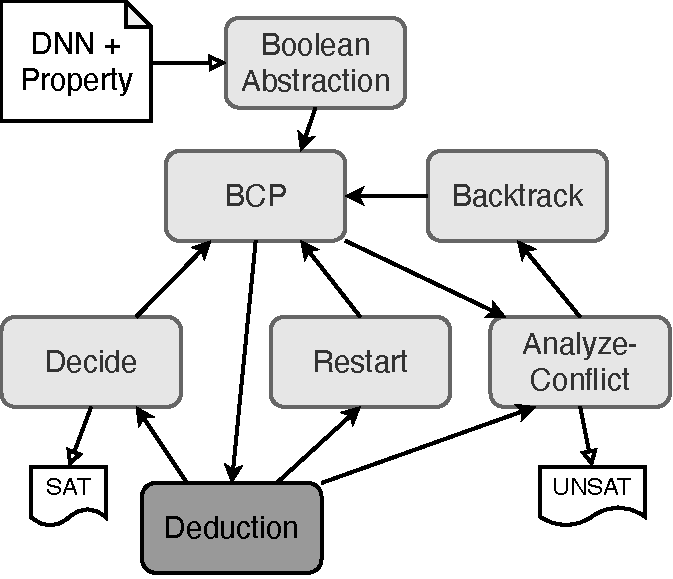
\includegraphics[width=0.4\linewidth]{figure/arch.pdf}
    \caption{\label{fig:overview} The \neuralsat{} DPLL(T) Algorithm.} 
\end{figure}


\autoref{fig:overview} gives an overview of \neuralsat{}, which consists of standard DPLL components (light shades) and the theory solver (dark shade).
\neuralsat{} first constructs a propositional formula over Boolean variables that represent the activation status of neurons (\emph{Boolean Abstraction}). Clauses in the formula assert that each neuron, e.g., neuron $i$, is active or inactive, e.g., $v_i \vee \overline{v_i}$.
This representation enables using standard DPLL to search for truth values satisfying these clauses and a DNN-specific theory solver to check the feasibility of truth assignments with respect to the constraints encoding the DNN and the property of interest.

\neuralsat{} now enters an iterative process to find a truth assignment---\emph{activation pattern} (\autoref{sec:activation-pattern})---satisfying the activation clauses.
First, \neuralsat{} assigns a truth value to an unassigned variable (\emph{Decide}), detects unit clauses caused by this assignment, and infers additional assignments (\emph{Boolean Constraint Propagation}).
Next, \neuralsat{} invokes the theory solver or T-solver (\emph{Deduction}), which uses LP solving and abstraction to check the satisfiability of the constraints of the current assignment with the property of interest. %The T-solver can also infer additional truth assignments.


If the T-solver confirms satisfiability, \neuralsat{} continues with new assignments (\emph{Decide}). Otherwise, \neuralsat{} detects a conflict   (\emph{Analyze Conflict}) and learns clauses to remember it and backtrack to a previous decision  (\emph{Backtrack}).
If \neuralsat{} detects local optima, it would restart (\emph{Restart}) the search by clearing all decisions that have been made, but save the conflict clauses learned so far to avoid reaching the same state in the next runs.
Restarting especially benefits challenging DNN problems by enabling better clause learning and exploring different decision orderings.

This iterative process repeats until \neuralsat{} can no longer backtrack, and returns \unsat{}, indicating the DNN has the property, or it finds a total assignment for all boolean variables, and returns \sat{}. % (and the user can query \neuralsat{} for a counterexample).

\autoref{sec:neuralsat-alg} provides more details on the \neuralsat{} algorithm, describing the main components of \neuralsat{} and how they work together to verify DNNs.


\section{Illustration}
\begin{example}\label{ex:neuralsat}
We use \neuralsat{} to prove that for inputs $x_1 \in [-1, 1], x_2 \in [-2,2]$ the DNN in Fig.~\ref{fig:dnn} produces the output $x_5 \le 0$.
\neuralsat{} takes as input the formula $\alpha$ representing the DNN:

\begin{equation*}%\label{eq:ex}
\begin{aligned}
  x_3 &=  \relu{-0.5x_1 + 0.5x_2 + 1} ~\land\\
  x_4 &= \relu{x_1 + x_2 - 1} ~\land\\
  x_5 &= -x_3 + x_4 - 1.0
\end{aligned}
\end{equation*}
and the formula $\phi$ representing the property:

\begin{equation*}\label{eq:valid_prop}
    \phi : -1\le x_1 \le 1 \land -2 \le x_2 \le 2 \quad\Rightarrow\quad x_5 \le 0.
\end{equation*}

To prove $\alpha \Rightarrow \phi$, \neuralsat{} needs to show  that \emph{no} values of $x_1,x_2$ satisfying the input properties would result in $x_5 > 0$. In other words, \neuralsat{} needs to return \texttt{unsat} for: 
\begin{equation}\label{eq:negprop}
  \alpha\; \land\; -1 \le x_1 \le 1     \;\land\; -2 \le x_2 \le 2   \;\land\; x_5 > 0.
\end{equation} 

\textbf{Notation:} In the following, we write $x \mapsto v$ to denote that the variable $x$ is assigned with a truth value $v \in \{T,F\}$. This assignment can be either decided by \texttt{Decide} or inferred by \texttt{BCP}. We also write $x@dl$ and  $\overline{x}@dl$ to indicate the respective assignments $x \mapsto T$ and $x \mapsto F$  at decision level $dl$.

\paragraph{Boolean Abstraction} First, \neuralsat{} creates two Boolean variables $v_3$ and $v_4$ to represent the
%(pre-ReLU)
activation status of the hidden neurons $x_3$ and $x_4$, respectively. For example, $v_3=T$ means $x_3$ is \texttt{active} and thus gives the constraint $-0.5x_1 + 0.5x_2 + 1 > 0$. Similarly, $v_3=F$ means $x_3$ is \texttt{inactive} and therefore gives $-0.5x_1 + 0.5x_2 + 1\le 0$. Next, \neuralsat{} forms two clauses  $\{v_3 \lor \overline{v_3} \;;\; v_4 \lor \overline{v_4}\}$ ensuring that these variables are either \texttt{active} or \texttt{inactive}.


%Now, \neuralsat{} searches for truth assignments for activation variables to satisfy the clauses. %(and later check that they also satisfy the constraints of DNN implied by these variables and the properties to be proved).
%We summarize the five iterations \neuralsat{} uses to determine that no such assignment exists (i.e., \texttt{unsat}).

%We show how \neuralsat{} proves that network in Fig.~\ref{fig:dnn} has property in ~\autoref{eq:valid_prop}, i.e., for any inputs $x_1 \in [-1, 1], x_2 \in [-2,2]$, the network produces the output $x_5 \le 0$. 

% \textbf{SAT formulation} \neuralsat{} first encodes the verification task into an SMT checking problem as described in \S\ref{sec:nnverif} by representing the network in Fig.~\ref{fig:dnn}b as the formula:

% and negating of the property in Eq~\ref{eq:valid_prop}:
% \begin{equation}\label{eq:negprop}
%         -1 \le x_1 \le 1     \;\land\; -2 \le x_2 \le 2   
%         \;\land\; x_5 > 0.
% \end{equation} 

%\hd{I might use different weight for DNN to trigger some technique in the tool.}\tvn{yes, that's fine, make it as easy to illustrate as possible, but should also be challenging enough to require at least 2-3 iterations.  Also good to demonstrate 2 cases:  sat and unsat. For example, focus on say unsat,  and then after illustrating that,  make a new subsection and change something so that it would be sat and briefly mentions how \neuralsat{} would work to return sat}\tvn{\tool is complex, so instead of using the Dynaplex example, which is a bit too easy,  maybe look at the illustrative example for the GenTree's paper---it has more details.  Or even look at the Reluplex's illustrative example in the Survey paper}.

%We use an example\tvn{Hai: create an example, may be use the DNN from PA4 (or subset of that DNN)} to demonstrate how \neuralsat{} works.  Fig.~\ref{fig:ex} shows a small DNN ....  


% \begin{figure}
%   \centering
%   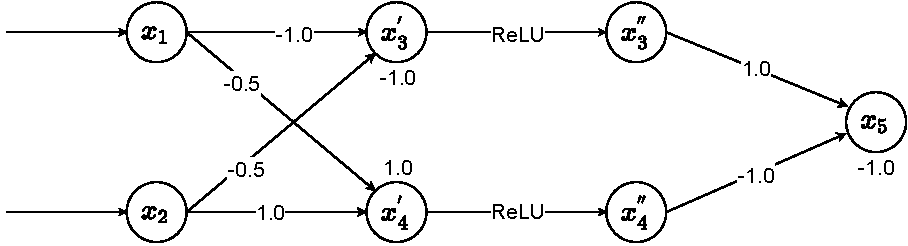
\includegraphics[width=0.7\linewidth]{figure/example-b.pdf}
%   \caption{Simple FNN with ReLU activation.} \label{fig:ex}
% \end{figure}

%\hd{Step 0: About the network - copy somewhere, need to rewrite}
%\textbf{Running example}

%We use an example of simple fully-connected feed-forward neural network with %ReLU activation shown in Fig.~\ref{fig:dnn} to demonstrate how \neuralsat{} works. 
%This network has already been trained and we have the learned weights and bias shown in the figure. 
%The network consists of three layers: an input layer, a hidden layer, and an output layer with two neurons each. 
%The weights on the edges represent the learned coefficients of the weight matrix used by the affine transformations done at each layer. The learned bias for each neuron is shown above or below it. 


% \neuralsat{} aims to find an assignment satisfying the conjunction of the formulae in ~\autoref{eq:ex} and~\ref{eq:negprop}. Such an assignment represents a counterexample violating the property, i.e., within the given ranges but does not satisfy the output requirement.
% %If such an input does not exist, \neuralsat{} returns \texttt{unsat}, indicating the property is valid. Otherwise it returns \texttt{sat} and the input, which represents a counterexample violating the property.

% Next, from the formula in ~\autoref{eq:ex}, \neuralsat{} creates two Boolean variables $v_3$ and $v_4$ to represent the status of the hidden pre-ReLU neurons $x_3'$ and $x_4'$. For example, $v_3=T$ means the status of $x_3$ is \texttt{on}, i.e., $-x_1-0.5x_2-1>0$ and $v_3=F$ means $x_4=\texttt{off}$, i.e.,  $-x_1-0.5x_2-1>0$. \neuralsat{} also forms two initial clauses indicating the status variables must be either \texttt{on} or \texttt{off}: $v_3 \lor \overline{v_3} \;;\; v_4 \lor \overline{v_4}$.



% \begin{equation}\label{eq:newvars}
%     \begin{aligned}
%         v_3 \vee \overline{v_3} \\
%         v_4 \vee \overline{v_4} 
%     \end{aligned}
% \end{equation}




% \begin{table*}
%   \caption{\neuralsat{}'s run producing \texttt{unsat}. The notation $x@dl$ and $\overline{x}@dl$ mean the assignments $x \mapsto T$ and $x \mapsto F$ at decision level $dl$, respectively.}\label{tab:valid}
%   \centering
%   \footnotesize
%     \begin{tabular}{c|c|cc|c|cc}
%     \toprule
%     Iter & \textbf{BCP} & \multicolumn{2}{c|}{\textbf{DEDUCTION}}& \textbf{DECIDE} & \multicolumn{2}{c}{\textbf{ANALYZE-CONFLICT}} \\
%       &&Constraints&Bounds&&Backtrack&Learned Clauses\\
%       \midrule
%       Init &-& $I = -1 \le x_1 \le 1; -2 \le x_2 \le 2$ & $-1 \le x_1 \le 1; -2 \le x_2\le 2$ & - &-&$C = \{v_3 \lor \overline{v_3};\; v_4 \lor \overline{v_4}\}$\\
      
%       1 &-&$I$ & $ x_5 \le 1 $& $\overline{v_4}@1$&-&-\\
      
%       2 &-&$I; x_4=\texttt{off}$&$ x_5 \le -1$& - & 0 &  $C = C \cup \{v_4\}$\\
      
%       3 &$v_4@0$&$I; x_4=\texttt{on} $&$ x_3 \ge 0.5; x_5 \le 0.5$ & $v_3@0$&-&-\\
      
%       4 &-&$I; x_3=\texttt{on}; x_4=\texttt{on}$&-&- & \bf{-1} & $C = C\cup \{\overline{v_4}\}$\\
      
%       % 5 &$v_4@0$&$I; x_3=\texttt{on}; x_4=\texttt{on}$&-&- & \bf{-1}& $C = C \cup \overline{v_3}\lor \overline{v_4}$\\
      
%        \bottomrule
%     \end{tabular}
% \end{table*}

%The goal is to find an activation pattern---a truth assignment for these variables---that satisfies the conjunction of the clauses in~\autoref{eq:negprop}. Such an assignment represents a counterexample violating the property, i.e., within the given ranges but does not satisfy the output requirement. If no such assignment exists, \neuralsat{} returns \texttt{unsat}, indicating the property is valid.

\paragraph{DPLL(T) Iterations} \neuralsat{} searches for a satisfying \emph{activation pattern}---truth assignment for the Boolean variables to satisfy the clauses and the constraints they represent with respect to the formula in~\autoref{eq:negprop}.
For this example, \neuralsat{} uses four iterations, summarized in~\autoref{tab:valid}, to determine that no such assignment exists and the problem is thus \unsat{}.


\begin{table*}
    \centering
    \caption{\neuralsat{}'s run producing \unsat{}.}\label{tab:valid}
    \footnotesize
      \begin{tabular}{ccccccc}
      \toprule
      Iter & \textbf{BCP} & \multicolumn{2}{c}{\textbf{DEDUCTION}}& \textbf{DECIDE} & \multicolumn{2}{c}{\textbf{ANALYZE-CONFLICT}} \\
        &&Constraints&Bounds&&Bt&Learned Clauses\\
        \midrule
        Init &-& $I = -1 \le x_1 \le 1; $& $-1 \le x_1 \le 1;$  & - &-&$C = \{v_3 \lor \overline{v_3};\; v_4 \lor \overline{v_4}\}$\\
        && $-2 \le x_2 \le 2$ & $-2 \le x_2\le 2$& & & \\
        1 &-&$I$ & $ x_5 \le 1 $& $\overline{v_4}@1$&-&-\\
        
        2 &-&$I; x_4=\texttt{off}$&$ x_5 \le -1$& - & 0 &  $C = C \cup \{v_4\}$\\
        
        3 &$v_4@0$&$I; x_4=\texttt{on} $&$ x_3 \ge 0.5; x_5 \le 0.5$ & $v_3@0$&-&-\\
        
        4 &-&$I; x_3=\texttt{on}; x_4=\texttt{on}$&-&- & \bf{-1} & $C = C\cup \{\overline{v_4}\}$\\
        
        % 5 &$v_4@0$&$I; x_3=\texttt{on}; x_4=\texttt{on}$&-&- & \bf{-1}& $C = C \cup \overline{v_3}\lor \overline{v_4}$\\
        
         \bottomrule
      \end{tabular}
  \end{table*}

  
%\emph{Initially}, the set of constraints  consists of the given bounds over the inputs, and the set of the clauses contains the two clauses in ~\autoref{eq:newvars}.

In \emph{iteration 1}, as shown in~\autoref{fig:overview}, \neuralsat{} starts with \texttt{BCP}, which has no effects because the current clauses and (empty) assignment produce no unit clauses.
In \texttt{Deduction}, \neuralsat{} uses an LP solver to determine that the current set of constraints, which contains just the initial input bounds, is feasible\footnote{We use the terms feasible, from the LP community, and satisfiable, from the SAT community, interchangeably.}. \neuralsat{} then uses abstraction to approximate an output upper bound $x_5 \le 1$ and thus deduces that satisfying the output $x_5 >0$ might be feasible. \neuralsat{} continues with \texttt{Decide}, which uses a heuristic to select the unassigned variable $v_4$ and sets $v_4=F$---essentially a \emph{guess} that neuron $x_4$ is inactive. \neuralsat{} increments the decision level ($dl$) to 1 and associates $dl=1$ to the assignment, i.e., $\overline{v_4}@1$.


In \emph{iteration 2}, \texttt{BCP} again has no effect because it does not detect any unit clauses. In \texttt{Deduction}, \neuralsat{} determines that current set of constraints, which contains $x_1 + x_2 - 1 \le 0$ due to the assignment $v_4\mapsto F$ (i.e., $x_4=\texttt{off}$), is feasible. \neuralsat{} then approximates a new output upper bound $x_5\le -1$, which means satisfying the output $x_5 > 0$ constraint is \emph{infeasible}.

\neuralsat{} now enters \texttt{AnalyzeConflict} and determines that $v_4$ causes the conflict ($v_4$ is the only variable assigned so far).  From the assignment $\overline{v_4}@1$, \neuralsat{} learns a ``backjumping'' clause $v_4$, i.e., $v_4$ must be $T$. \neuralsat{} now backtracks to $dl$ $0$ and erases all assignments decided \emph{after} this level. Thus, $v_4$ is now unassigned and the constraint  $x_1 + x_2 - 1 \le 0$ is also removed.

In \emph{iteration 3}, \texttt{BCP} determines that the learned clause is also a unit clause $v_4$ and infers $v_4@0$. In \texttt{Deduction}, we now have the new constraint $x_1 + x_2 - 1 > 0$ due to $v_4 \mapsto T$ (i.e., $x_4=\texttt{on}$).  With the new constraint, \neuralsat{} 
%\hd{tightens input bounds and get $0 \le x_2 \le 2$, then} 
approximates the output upper bound $x_5 \le  0.5$, which means $x_5>0$ might be satisfiable.
Also, \neuralsat{} computes new bounds $0.5 \le x_3 \le 2.5$ and $0 < x_4 \le 2.0$, and deduces that $x_3$ must be positive because its lower bound is 0.5. 
Thus, \neuralsat{} has a new assignment $v_3@0$ ($dl$ stays unchanged due to the implication). 
This new assignment inference from the T-solver is known as \emph{theory propagation} in DPLL(T).

In \emph{iteration 4}, \texttt{BCP} has no effects because we have no new unit clauses.  In \texttt{Deduction}, \neuralsat{} determines that the current set of constraints, which contains the new constraint $-0.5x_1+0.5x_2+1 > 0$ (due to $v_3 \mapsto T$), is \emph{infeasible}. Thus, \neuralsat{} enters \texttt{AnalyzeConflict} and determines that $v_4$, which was set at $dl=0$ (by \texttt{BCP} in iteration 3), causes the conflict. 
\neuralsat{} then learns a clause $\overline{v_4}$ (the conflict occurs due to the assignment $\{v_3 \mapsto T; v_4 \mapsto T\}$, but $v_3$ was implied and thus making $v_4$ the conflict).
However, because $v_4$ was assigned at decision level 0, \neuralsat{} can no longer backtrack and thus sets $dl=-1$ and returns \unsat{}, i.e , the property is valid.


% Note that because we backtrack to $dl=0$, we do not erase the assignment $v_3=T$ because it was decided at $dl=0$ (by BCP in iteration 3).

% In \emph{iteration 5}, because of the new clause $\overline{v_3} \lor v4$ and $v_3$ is already set to $T$, BCD infers $v_4=T$ at dl=0.  In DEDUCTION, \neuralsat{} determines that set of constraints, which contains $-0.5x_1+x_2+1> 0$ for $x_4'=\texttt{on}$ (because $v_4=T$), is infeasible. In ANALYZE-CONFLICT, \neuralsat{} determines $v_4$ causes the conflict  and learns the new clause $\overline{v3} \lor \overline{v4}$ (because the current assignment $v_3=1;v_4=1$ cause the conflict).
% \neuralsat{} then sets $dl=-1$ (because $v_4=T$ was decided at level 0) and realizes that it can no longer backtrack, and thus returns \texttt{unsat}.  Note that we can also see that the learned clauses $\{v_3, \overline{v_3} \lor v_4, \overline{v_3} \lor \overline{v_4}\}$ are not satisfiable.

%\tvn{do we use restart for this example?}\hd{we do not, it would be very long as in FSE paper.}

%Note that this example is too simple to illustrate the use of \emph{restart}, which is described in~\autoref{sec:restart-tree} and~\autoref{sec:restart} and crucial for more complicated and nontrivial problems.
\end{example}






%% \textbf{Discussion}
%% Testing. Does not affect soundness and helps with completeness.
%% Since the procedure is sampling-based, it is applicable to neural networks with any type of activation function.
%% Does not affect performance of DPLL(T) and helps quickly knock out easy instances as shown in experimentation.
%% Used by some verification tools. \tvn{SAT/SMT solvers also do that?} \hd{Not SAT/SMT solver, other verifiers, like ERAN, abcrown, also do that}


%% The falsification algorithm is \textbf{sound} but \textbf{not complete}. 
%% When a falsifying input has been found by our algorithm, it terminates by declaring the network as \textbf{unsafe} and the reported counterexample indeed violates the safety property of the network. 
%% However, when it terminates before finding any falsifying input, one cannot guarantee the absence of any falsifying input and consequently, the safety of the network with respect to the property.

%% % \subsection{Other DPLL components}

%% % Describe other DPLL components (BCP, Decide using VSIDS, etc).  If they are complicated enough,  give it its own section.  

%% \subsection{Properties of \tool{}}

%% \textbf{Sound} \tool{} is sound because the main DPLL algorithm is sound, also the abstraction domain are over-approximated techniques, then they are sound. 

%% \textbf{Complete} Deduce/Theory solver calls LP solver over the reals?

%% \textbf{Complexity} The worst-case complexity of \tool{} is exponential in the number of neurons. More specifically, the algorithm works by assigning activation status for each neuron (either on or off) and thus in the worst-case \tool{} will try all $2^n$ possible combinations of assignments, where $n$ is the number of neurons.  %Moreover, for each combination, \tool{} also performs linear programming solving to check for assignment feasibility.

%% \hd{
%%     This section is duplicated elsewhere
    
%%     \subsection{Difference between of \tool{} and BaB-based verifiers}
    
%%     For example, the network has 5 neurons corresponding to 5 variables, e.g., $\{v_1, v_2, v_3, v_4, v_5\}$. 
%%     Also, \tool{} already assigned $v_1@0, v_2@0, v_3@0$, and suppose that it has generated a conflict clause $c = \overline{v_2} \lor v_4 \lor v_5$.
%%     If \tool{} continue to split an unsigned neurons (e.g., $v_4$ or $v_5$), e.g., \tool{} chooses $v_4$.
%%     If $v_4@1$, there will be 2 cases for $v_5$, e.g., $v_5@2$ and $\overline{v_5}@2$.
%%     If $\overline{v_4}@1$, there will be only one case for $v_5$, that is, $v_5@2$, because of the generated conflict clause $c$.
%%     In total, there will be \textbf{at most} 3 splits to check with help of the learnt conflict clause $c$.
    
%%     In the other hand, if the BaB-based algorithm reached the same state above, e.g, there remains 2 unstable neurons $v_4, v_5$, and they need to check \textbf{at most} 4 splits.


%%     In short, we might be able to decrease some iterations with the help of the conflict clause learning technique.
%% }




\section{\tool{}'s Optimizations}\label{sec:optimizations}

\tool{}implements several optimizations to improve the performance of the search. First are the common optimizations used by other DNN verifiers, such as input splittings (\autoref{chap:common-engineering}) and adversarial attacks (\autoref{chap:adversarial-attacks}). In addition, \neuralsat{} implements several unique optimizations~\cite{duong2024harnessing} to improve the performance of the search. These are neuron stability, restart tree, and restart.


\subsection{Neuron Stability}\label{sec:stabilization}
A neuron is \emph{stable} if its activation status does not change regardless of the input values. In contrast, a neuron is \emph{unstable} if its activation status can change depending on the input values. For example, in the DNN in Fig.~\ref{fig:dnn}, \tvn{any neuron stable? or they are all unstable?}

The key idea in using neuron stability is that if we can determine that a neuron is stable,  we can assign the exact truth value for the corresponding Boolean variable instead of having to guess. This has a similar effect as \functiontextformat{BCP}---reducing mistaken assignments by \functiontextformat{Decide}---but it operates at the theory level instead of the propositional Boolean level.

%First, the T-solver creates a linear constraint system from the input assignment $\sigma$ and $\alpha \land \phi_{in} \land \overline{\phi_{out}}$, i.e., the formula in ~\autoref{eq:prob} representing the original problem  (line~\ref{line:lpsolver}).
%First, the T-solver creates a set of linear constraints representing ReLU activation for hidden neurons whose activation status have been decided.
%Next, those constraints are used in \textsc{Stabilize} for inferring status of neurons that are unassigned, \textsc{Deduce} then applies the polytope abstraction to check satisfiability.
%If the abstraction confirms the infeasibility, \textsc{Deduce} returns \texttt{False} so that \textsc{AnalyzeConflict} can analyze the assignment and and learn the conflict clause.
%Otherwise, the current assignment might be feasible and \textsc{Decide} continues to split more hidden neurons.


%\texttt{Stabilize} (Fig.~\ref{fig:alg} line~\ref{line:stabilize}) first creates linear constraints consisting of the DNN $\alpha$, the input \tvn{fillin} and output \tvn{fillin} conditions, and the current assignment $\sigma$. Next, it uses these constraints to generate a Mixed Integer Linear Programming (MILP) problem (~\autoref{eq:mip}), whose objective is compute a tighter lower and upper bounds for unstable neurons based on the current search state (i.e., the current assignment $\sigma$).

%the considered property into a set of constraints for
%The main goal of this process is to


%the boolean values activation status instead of
%that we can remove ReLU activation for hidden neurons whose activation status have been decided, each propositional variable in current assignment concretizes (removes) its corresponding constraints in MILP problem (~\autoref{eq:mip}) that helps solver reduce numbers of constraints and be able to tighten bounds further.



% \hd{Should mention about StabilizeCondition: \tool{} invokes Stabilize() after a number of iterations without improvement in Deduce step (abstraction), e.g, 10 iterations.}

%\tvn{candidate to remove}
%The complexity of this problem can increase exponentially with the number of ReLU neurons, so it would take long time to run even on a small network.
%In the previous work, \mipverify{}~\cite{tjeng2019evaluating} encoded the adversarial attack and verification of ReLU-based networks MIP problem, directly solved by existing MILP solvers (e.g., Gurobi).
%In this work, we do not use MILP for solving instances directly, instead we leverage the progressive bound tightening for determining tighter bounds for hidden neurons which is crucial for problem tractability: tight bounds strengthen the problem formulation and thus improve solve times~\cite{vielma2015mixed}.
%Furthermore, if we can prove that a neuron is stable, we can avoid splitting in the DPLL(T)-based search process.

%Theoretically, for ReLU-based networks, each neuron can either be \textit{active} (its input is positive) or \textit{inactive} (its input is negative so the output is 0), which can be encoded by discrete 0-1 variables.
%Those networks can be generally formulated into a MILP problem which has binary variables $a_j^{(i)}$ for an $j^{th}$ ReLU at layer $i$:

Stabilization involves the solution of a mixed integer linear program (MILP) system~\cite{tjeng2019evaluating}:
\begin{equation}
    \begin{aligned}
        &\mbox{(a)}\quad z^{(i)} = W^{(i)} \hat{z}^{(i-i)} + b^{(i)}; \\
        &\mbox{(b)}\quad y = z^{(L)};  x = \hat{z}^{(0)}; \\
        &\mbox{(c)}\quad \hat{z}_j^{(i)} \ge {z}_j^{(i)}; \hat{z}_j^{(i)} \ge 0; \\
        &\mbox{(d)}\quad a_j^{(i)} \in \{ 0, 1\} ;\\
        &\mbox{(e)}\quad \hat{z}_j^{(i)} \le {a}_j^{(i)} {u}_j^{(i)}; \hat{z}_j^{(i)} \le {z}_j^{(i)} - {l}_j^{(i)}(1 - {a}_j^{(i)}); \\
    \end{aligned}
    \label{eq:mip}
\end{equation}
where $x$ is input, $y$ is output, and $z^{(i)}$, $\hat{z}^{(i)}$, $W^{(i)}$, and $b^{(i)}$ are the pre-activation, post-activation, weight, and bias vectors for layer $i$.
The equations encode the semantics of a DNN as follows:
(a) defines the affine transformation computing the pre-activation value for a neuron in terms of outputs in the preceding layer;
(b) defines the inputs and outputs in terms of the adjacent hidden layers;
(c) asserts that post-activation values are non-negative and no less than pre-activation values;
(d) defines that the neuron activation status indicator variables that are either 0 or 1; and
(e) defines constraints on the upper, $u_j^{(i)}$, and lower, $l_j^{(i)}$, bounds of the pre-activation value of the $j$th neuron in the $i$th layer.
Deactivating a neuron, $a_j^{(i)} = 0$, simplifies the first of the (e) constraints to $\hat{z}_j^{(i)} \le 0$, and activating a neuron simplifies the second to $\hat{z}_j^{(i)} \le z_j^{(i)}$, which is consistent with the semantics of $\hat{z}_j^{(i)} = max(z_j^{(i)},0)$.

%Even if \functiontextformat{Stabilize} fails to stabilize, \tool{} still can solve problem by other components, e.g., parallel DPLL(T) search.



\SetKwFunction{GetUnassignedVariable}{GetUnassignedVariable}
\SetKwFunction{Sort}{Sort}

\begin{algorithm}[t]
    \footnotesize

    \Input{DNN $\alpha$, property $\phi_{in} \Rightarrow \phi_{out}$, current assignment $\sigma$, number of neurons for stabilization $k$}
    \Output{Tighten bounds for variables \textbf{not} in $\sigma$ (unassigned variables)}
    \BlankLine

    % \tcp{create an MILP solver based on ~\autoref{eq:mip}}
    $\model \leftarrow \MIP(\alpha, \phi_{in}, \phi_{out}, \sigma)$ \tcp{create model (~\autoref{eq:mip}) with  current assignment}

    $[v_1, ..., v_m] \leftarrow \GetUnassignedVariable(\sigma)$ \tcp{get all $m$ current unassigned variables} \label{line:find}


    $[v_1', ..., v_m'] \leftarrow \Sort([v_1, ..., v_m])$ \tcp{prioritize tightening order} \label{line:sort}
    $[v_1', ..., v_k'] \leftarrow \Select([v_1', ..., v_m'], k)$ \tcp{select top-$k$ unassigned variables, $k \le m$} \label{line:topk}

    \tcp{stabilize $k$ neurons in parallel}
    \Parfor{$v_i$ \textbf{in} $[v_1', ..., v_k']$}{
        \If(\tcp*[h]{lower is closer to 0 than upper, optimize lower first}){$(v_i.lower + v_i.upper) \ge 0$}{
            % \tcp{lower is closer to 0 than upper, optimize lower first}
            $\Maximize(\model, v_i.lower)$ \tcp{tighten lower bound of $v_i$} \label{line:maximize1}
            \If(\tcp*[h]{still unstable}){$v_i.lower < 0$}{
                $\Minimize(\model, v_i.upper)$ \tcp{tighten upper bound of $v_i$} \label{line:minimize1}
            }
        }
        \Else(\tcp*[h]{upper is closer to 0 than lower, optimize upper first}){
            % \tcp{upper is closer to 0 than lower, optimize upper first}
            $\Minimize(\model, v_i.upper)$ \tcp{tighten upper bound of $v_i$} \label{line:minimize2}
            \If(\tcp*[h]{still unstable}){$v_i.upper > 0$}{
                $\Maximize(\model, v_i.lower)$ \tcp{tighten lower bound of $v_i$} \label{line:maximize2}
            }
        }
    }
    \vspace*{-0.2in}
    \caption{\texttt{Stabilize}}
    \label{fig:stabilize}
\end{algorithm}



\autoref{fig:stabilize} describes Stabilize solves this equation system.
First,  a MILP problem is created from the current assignment, the DNN, and the property of interest using formulation in ~\autoref{eq:mip}.
Note that the neuron lower (${l}_j^{(i)}$) and upper bounds (${u}_j^{(i)}$) can be quickly computed by polytope abstraction.

Next, it collects a list of all unassigned variables which are candidates being stabilized (line~\ref{line:find}).
In general, there are too many unassigned neurons, so
\functiontextformat{Stabilize} restricts consideration to $k$ candidates.
Because each neuron has a different impact on abstraction precision we prioritize the candidates.
In \functiontextformat{Stabilize}, neurons are prioritized based on their interval boundaries (line~\ref{line:sort}) with a preference for neurons with either lower or upper bounds that are closer to zero.
The intuition is that neurons with bounds close to zero are more likely to become stable after tightening.

We then select the top-$k$ (line~\ref{line:topk}) candidates and seek to further tighten their interval bounds.
The order of optimizing bounds of select neurons is decided by its boundaries, e.g., if the lower bound is closer to zero than the upper bound then the lower bound would be optimized first.
These optimization processes, i.e., \functiontextformat{Maximize} (line~\ref{line:maximize1} or line~\ref{line:maximize2}) and \functiontextformat{Minimize} (line~\ref{line:minimize1} or line~\ref{line:minimize2}), are performed by an external LP solver (e.g., Gurobi~\cite{gurobi}).

%Note that the work in~\cite{tjeng2019evaluating} uses the MILP system in ~\autoref{eq:mip} to encode the entire verification problem and thus is limited to the encodings of small networks that can be handled by an LP solver.
%This MILP system is used by~\cite{tjeng2019evaluating} to encode the entire verification problem. It is passed to an LP solver to optimize the output of the network with respect to the the property of interest.
%This approach only works small networks whose constraints can be handled by LP solving.
%In contrast, \tool{} creates this system based on the current assignment, which has significantly fewer constraints.
%Moreover, we only use the computed bounds of hidden neurons from this system, and thus even if it cannot be solved, \tool{} will still continue.



\begin{example}
  \tvn{Need a concrete example here.  Use the DNN in Fig.~\ref{fig:dnn} and create the MILP system in ~\autoref{eq:mip}.}
\end{example}

\subsubsection{Parallel Search}\label{sec:parallel-search}
% Things need to write about
% \begin{itemize}
%     \item [+] how to parallelize DPLL: remove backtrack, compute both branches
%     \item [+] how to use learned clauses: run several times until problem is solved or reaches timeout, save conflict clauses before restarting and use them as initial clauses for next runs
%     \item [!] non-chronological backtracking isn't supported yet, need more engineering to handle this sort of backtracks
% \end{itemize}


%\tvn{this section is short. Add some more, may be some small examples (recall in the POPL paper we have various examples describing various DPLL components).  Does the tree in Fig1. applicable here?  If so you can refer to it. }
%\hd{it appears that's purely engineering to me, shouldn't be focused too much}\tvn{just write what engineerings were used here to help people understand how it works.  Also describe how this removes the need for Backtracking}
% We adopt the idea of Distributed tree search (DTS) algorithm which is a class of algorithms for searching values in an efficient and distributed manner~\cite{ferguson1988distributed}.
% \matt{I woud cite DTS.}
% Their purpose is to iterate through a tree by working along multiple branches in parallel and merging the results of each branch into one common solution, in order to minimize time spent searching for a value in a tree-like data structure.
% DPLL(T) is tree-search problem in each internal nodes is actually an activation pattern containing conditions values along the path from root to such node.
% \matt{replace path condition with activation pattern throughout the paper}
% The arrival of many-core machines leads to new possibilities for SAT solving.
% \matt{What techniques do the parallel SAT people use, i.e., \cite{le2017painless}, we should relate our solution to theirs.}
% Parallel SAT solving rely on two concepts: parallelization strategy and learnt clause exchanges.
% Two main parallelization methods have been developed: Portfolio~\cite{hamadi2010manysat} and Divide-and-Conquer~\cite{le2017painless}.
% The main idea of Portfolio is to run sequential solvers working in parallel on the entire formula, in a competitive way, aiming at increasing the probability of finding a solution using the diversification.
% The Divide-and-Conquer (DnC) approach is based on splitting the search space in disjoint subspaces that are solved independently in parallel by different workers.
% If a subspace is proven sat then the initial formula is sat.
% The formula is unsat if all the subspaces are unsat.
% The challenging points of the divide-and-conquer mechanism are:
% dividing the search space, balancing jobs between workers, and exchanging learnt clauses.

% We follow the DnC scheme
The DPLL(T) process in \tool{} is designed as a tree-search problem where each internal node encodes an \textit{activation pattern} defined by the variable assignments from the root.
To parallelize DPLL(T), we adopt a beam search-like strategy which combines distributed search from Distributed Tree Search (DTS) algorithm~\cite{ferguson1988distributed} and Divide and Conquer (DNC)~\cite{le2017painless} paradigms for splitting the search space into disjoint subspaces that can be solved independently.
At every step of the search algorithm, we select up to $n$ nodes  of the DPLL(T) search tree to create a beam of width $n$.
This splits (like DNC) the search into $n$ subproblems that are independently processed.  Each subproblem extends the tree by a depth of 1.

Our approach simplifies the more general DNC scheme since the $n$ bodies of the \textbf{parfor} on line~\ref{line:parfor} of Fig.~\ref{fig:alg} are roughly load balanced.
While this is a limited form of parallelism, it sidesteps one of the major roadblocks to DPLL parallelism -- the need to efficiently synchronize across load-imbalanced subproblems~\cite{le2017painless,le2019modular}.

In addition to raw speedup due to multiprocessing, parallelism accelerates the sharing of information across search subspaces, in particular learned clause information for DPLL. In \tool{}, we only generate independent subproblems which eliminates the need to coordinate their solution. When all subproblems are complete, their conflicts are accumulated, Fig.~\ref{fig:alg} line~\ref{line:analyze_conflict},  to inform the next round of search.
As we show in \S\ref{sec:eval}, the engineering of this form of parallelism in DPLL(T) leads to substantial performance improvement.

\subsection{Restart}

\SetKwFunction{threshold}{threshold}
\SetKwFunction{maxvisited}{max\_visited}
\SetKwFunction{maxremaining}{max\_remaining}
\SetKwData{implicationgraph}{igraph}


% \begin{algorithm}
%     \small

%     \Input{TBD}
%     \Output{TBD}
%     \BlankLine

%     $\threshold \leftarrow 3$ \tcp{predefined maximum number of restarts}
%     $\maxvisited \leftarrow 200000$ \tcp{predefined maximum number of visited nodes}
%     $\maxremaining \leftarrow 30000$ \tcp{predefined maximum number of remaining nodes}

    % \tcp{create an MILP solver based on ~\autoref{eq:mip}}
    % $\model \leftarrow \MIP(\alpha, \phi_{in}, \phi_{out}, \sigma)$ \tcp{create model (~\autoref{eq:mip}) with  current assignment}

    % $[v_1, ..., v_m] \leftarrow \GetUnassignedVariable(\sigma)$ \tcp{get all $m$ current unassigned variables} \label{line:find}


    % $[v_1', ..., v_m'] \leftarrow \Sort([v_1, ..., v_m])$ \tcp{prioritize tightening order} \label{line:sort}
    % $[v_1', ..., v_k'] \leftarrow \Select([v_1', ..., v_m'], k)$ \tcp{select top-$k$ unassigned variables, $k \le m$} \label{line:topk}

    % \tcp{stabilize $k$ neurons in parallel}
    % \For{$v_i$ \textbf{in} $[v_1', ..., v_k']$}{
    %     \If(){$(v_i.lower + v_i.upper) \ge 0$}{
    %         \tcp{lower is closer to 0 than upper, optimize lower first}
    %         $\Maximize(\model, v_i.lower)$ \tcp{tighten lower bound of $v_i$}
    %         \If(){$v_i.lower < 0$}{
    %             \tcp{still unstable}
    %             $\Minimize(\model, v_i.upper)$ \tcp{tighten upper bound of $v_i$}
    %         }
    %     }
    %     \Else{
    %         \tcp{upper is closer to 0 than lower, optimize upper first}
    %         $\Minimize(\model, v_i.upper)$ \tcp{tighten upper bound of $v_i$}
    %         \If(){$v_i.upper > 0$}{
    %             \tcp{still unstable}
    %             $\Maximize(\model, v_i.lower)$ \tcp{tighten lower bound of $v_i$}
    %         }
    %     }
    % }
%     \caption{\texttt{Reset}}
%     \label{fig:restart}
% \end{algorithm}

As with any stochastic algorithm, \tool{} would perform poorly if it gets into a subspace of the search that does not quickly lead to a solution, e.g., due to choosing a bad sequence of neurons to split~\cite{ferrari2022complete,wang2021beta,de2021improved}.
%In the development of modern SAT solver (e.g.PicoSAT~\cite{biere2008picosat}), researchers has realized most practical problems, even very large or complex, can be easily solved if they follow
This problem, which has been recognized in early SAT solving, motivates the introduction of restarting the search~\cite{gomes1998boosting} to avoid being stuck in such a \emph{local optima}. %This kind of heavy-tail behavior was also the motivation in the original publication on restarts \cite{}.


%In our context where easy SAT instances are usually falsified by external adversarial attack (e.g., PGD~\cite{madry2017towards}), or easy UNSAT instances are often verified within few iterations (e.g., a single iteration), we adopt restart schedule to avoid local optima during search process for ``hard'' problems (at certain points, the abstraction would not be improved or rarely improved).
%Moreover, previous related work showed that the order of making decisions had a great impact to their performance, hence, we hope that after restarting and decision heuristic is changed, \tool{} can follow other search directions toward the goal.

%\tvn{I am not so sure about listing all these numbers. Do we have to write about them here?}\hd{I think so, we can neglect those number too, those are heuristically selected and we didn't change them, different numbers might have different performances.}
\tool{} uses a simple restart heuristic that triggers a restart when either the number of processed assignments (nodes) exceeds a pre-defined number or the number of remaining assignments that need be checked exceeds a pre-defined threshold. % (e.g, 5000). (e.g, 20000)
% It also has a fast restart on the \textit{first} run when it detects a number of consecutive iterations (e.g., 10) without any improvement in abstraction steps.
%The period of restart is repeated until exceed a predefined maximum number of restarts (e.g., 3).
%These thresholds are chosen heuristically based on our experience. %and subject to change and performance of \tool{} might vary depending on those numbers.
After a restart, \tool{} avoids using the same decision order of previous runs (i.e., it would use a different sequence of neuron splittings). It also resets all internal information except the learned conflict clauses, which are kept and reused as these are \textit{facts} about the given constraint system.
This allows a restarted search to quickly prune parts of the space of assignments.
Although restarting may seem like an engineering aspect, it plays a crucial role in stochastic algorithms, and helps \neuralsat{} reduce verification time for challenging problemsk.

%In addition, to avoid revisiting the same search space over and over again, the decision  is changed at the beginning of every new run and conflict clauses learned so far are saved and never deleted.

% \hd{Why are restarts beneficial?}




\section{\tool{} vs. BaB}\label{sec:restart-tree}


\begin{figure}[t]
    \begin{minipage}[b]{\textwidth}
    \centering
        \begin{minipage}[t]{0.495\textwidth}
            \centering
            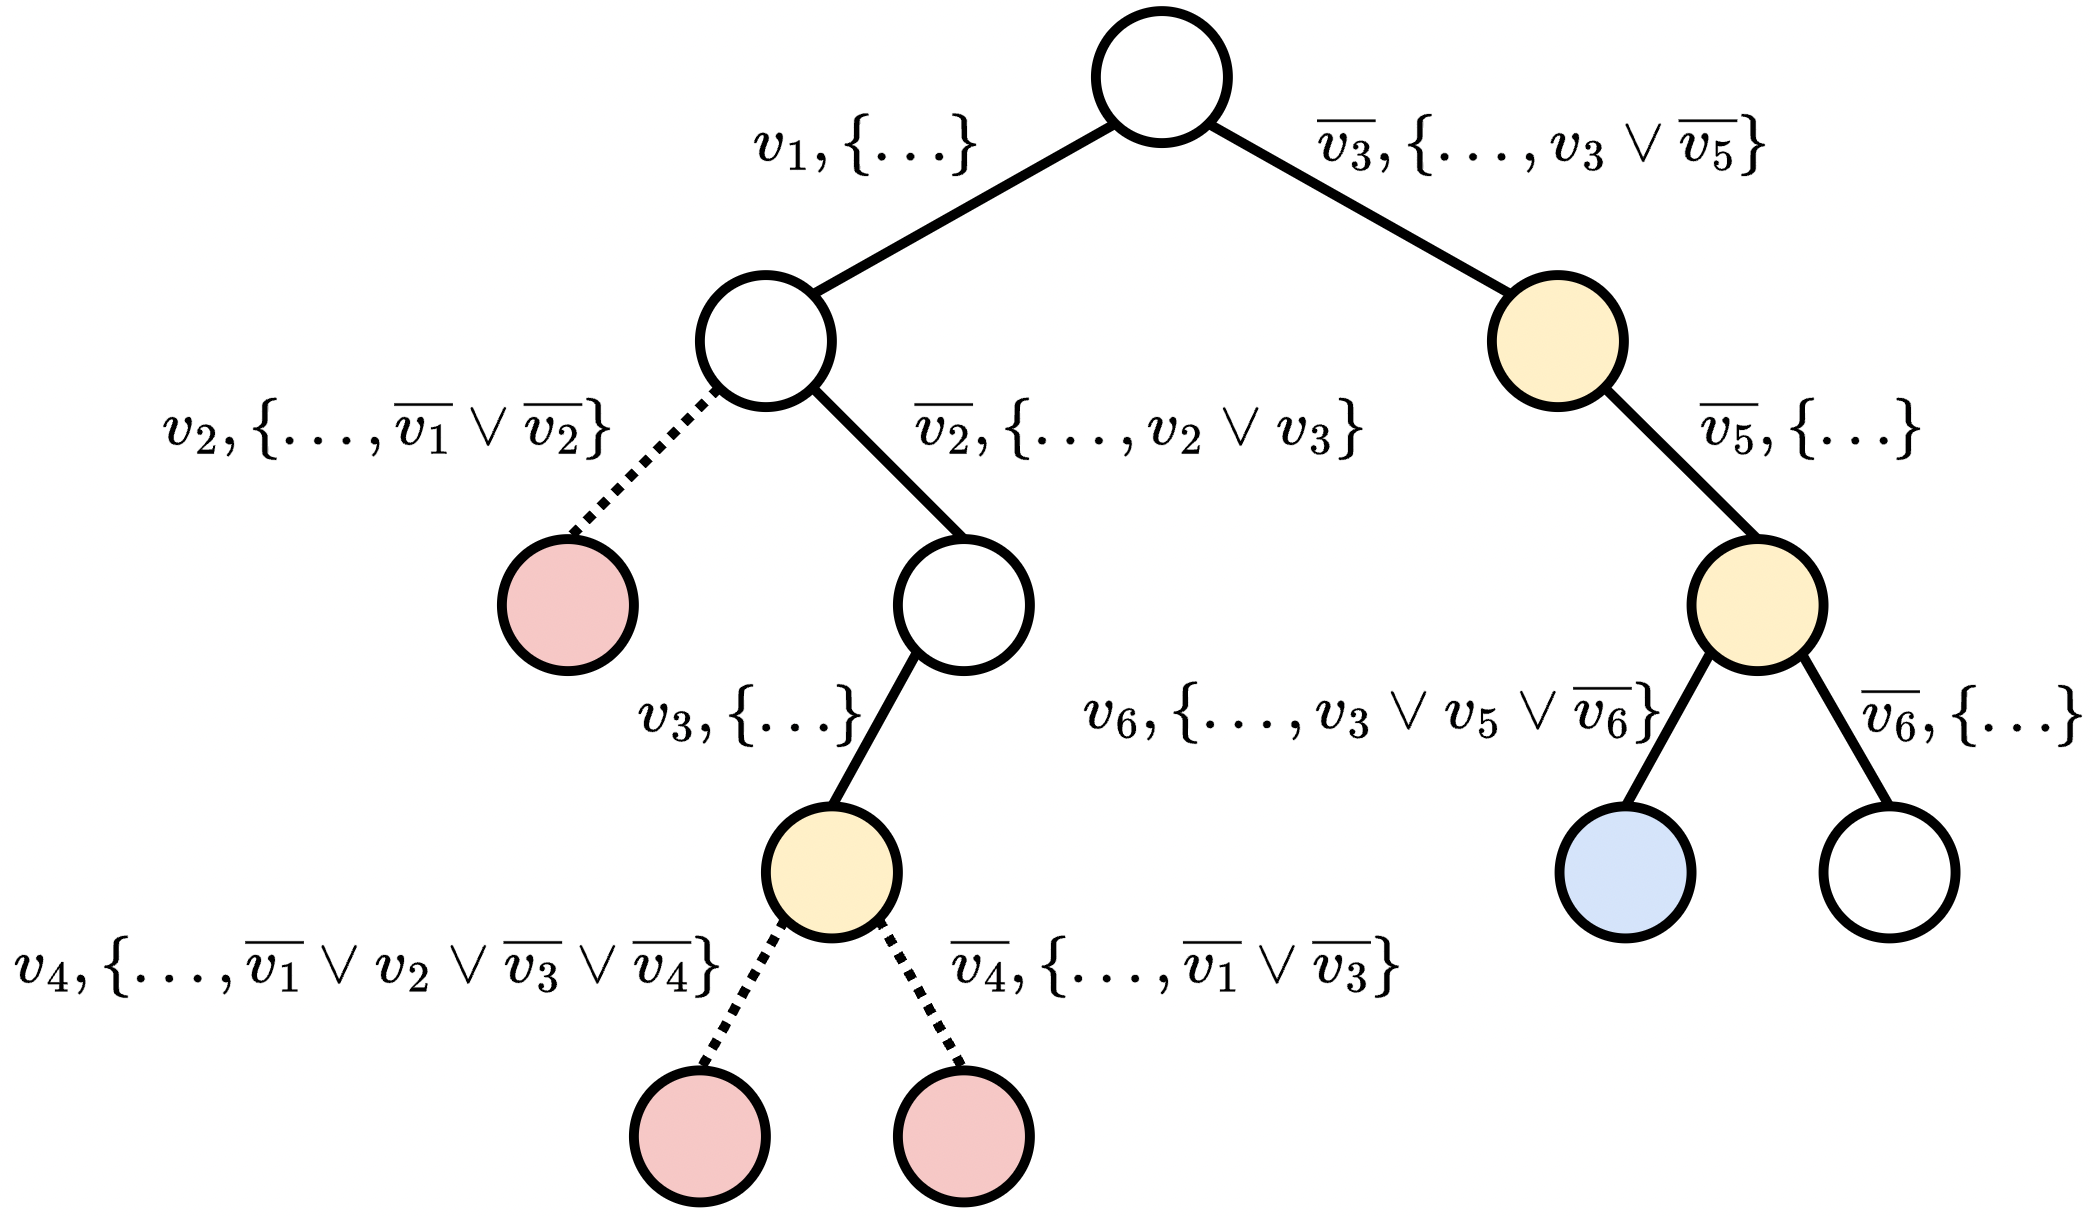
\includegraphics[width=\linewidth]{figure/cdcl-tree-clause.png}
            % 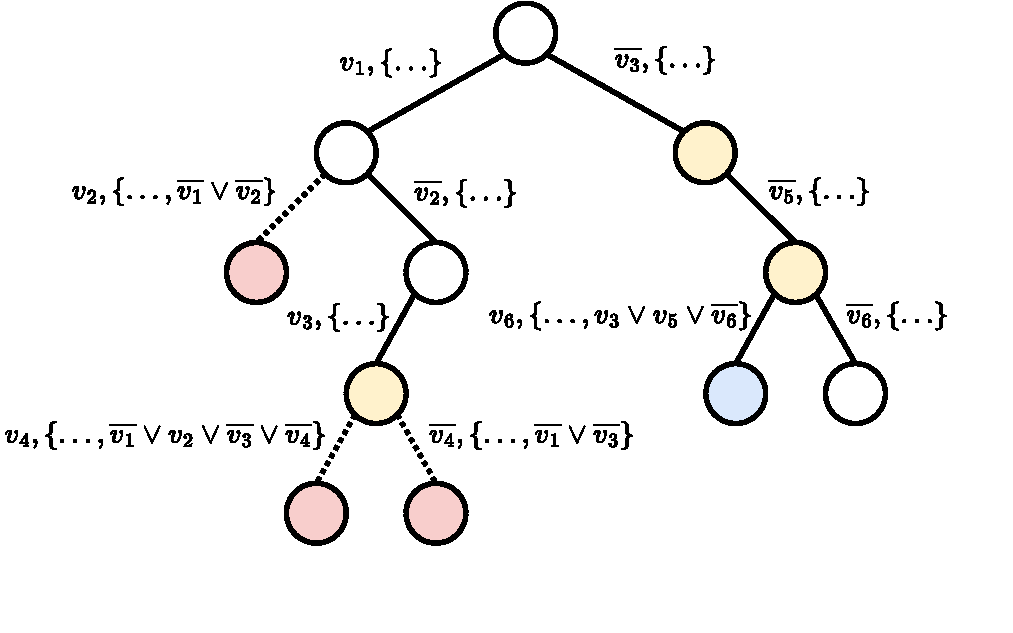
\includegraphics[width=\linewidth]{figure/cdcl-tree-clause.pdf}
            \caption*{(a) \tool{}}
        \end{minipage}
        % \hspace{0.5cm}
        \hfill
        \begin{minipage}[t]{0.44\textwidth}
            \centering
            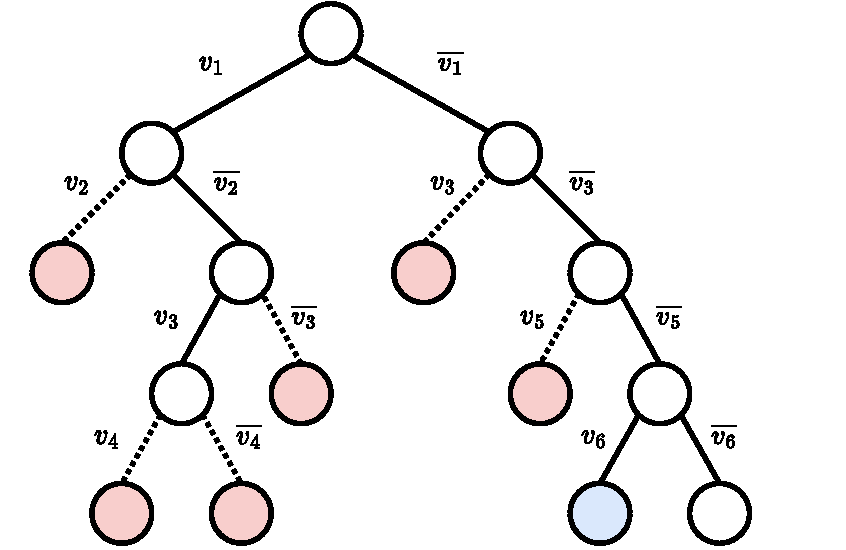
\includegraphics[width=\linewidth]{figure/none-cdcl-tree.pdf}
            \caption*{(b) Others}
        \end{minipage}
        % \hfill
        \vspace{-0.1in}
        \caption{Search tree explored by \tool{} (a) and other verifiers (b) during a verification run.
        \tvn{Hai, instead of other verifiers can we say this search tree is for a native/general BaB approach?}
        The notation $\{...\}$ indicates learned clauses; red is  infeasibility; white is feasibility; yellow is BCP application; and blue is current consideration.
        The search tree of \tool{} is smaller than the tree of the other techniques because \tool{} was able to prune various branches, e.g., through BCPs (e.g., ${v_3}$ and $\overline{v_5}$) and non-chronological backtracks (e.g., $\overline{v_3}$).}
        % \hd{missing a paragraph writing about this figure.}\tvn{yes, may be in the overview or intro if appropriate}\hd{still thinking of incorporating learned clauses.}
        \label{fig:tree}
    \end{minipage}
\end{figure}

\tvn{TODO: talk about how \tool{} is BaB but has things such as CDCL to help prune the search space.}

%modern DPLL implementations restart the DPLL procedure whenever the search is not making enough progress according to some measure. The rationale behind this idea is that upon each restart, the additional knowledge of the search space compiled into the newly learned lemmas will lead the heuristics for Decide to behave differently, and possibly cause the procedure to explore the search space in a more compact way. The combination of learning and restarts has been shown to be powerful not only in practice, but also in theory. Essentially, any Basic DPLL derivation to FailState is equivalent to a tree-like refutation by resolution. But for some classes of problems tree-like proofs are always exponentially larger than the smallest general, that is, DAG-like, resolution ones [Bonet et al. 2000]. The good news is that DPLL with learning and restarts becomes again equivalent to general resolution with respect to such notions of proof complexity [Beame et al. 2003].




\tvn{rewrite: technically we don't split if the guess was right}
Note that this process of selecting and assigning (guessing) values to variables representing neurons is the \emph{branching} phase in BaB. It is also commonly called \emph{neuron splitting} because  it splits the search tree into subtrees corresponding into the assigned values (e.g., see~\autoref{sec:restart-tree}).





As mentioned in \autoref{sec:complexity}, ReLU-based DNN verification is NP-complete, and for difficult problem instances DNN verification tools often have to exhaustively search a very large space, making scalability a main concern for modern DNN verification.

%One major difference that sets \tool{} apart from other DNN approaches is how it tackles and prunes such large search space.

\autoref{fig:tree} shows the difference between \tool{} and another DNN verification tool (e.g., using the popular Branch-and-Bound (BaB) approach) in how they navigate the search space.  We assume both tools employ similar abstraction and neuron splitting.
Fig.~\ref{fig:tree}b shows that the other tool performs splitting to explore different parts of the tree (e.g., splitting $v_1$ and explore the branches with $v_1=T$ and $v_1=F$ and so on). Note that the other tool needs to consider the tree shown regardless if it runs sequentially or in parallel.

% \tvn{Hai, could you change the LaTeX neg to overline?}\hd{yes}
In contrast, \tool{} has a smaller search space shown in Fig.~\ref{fig:tree}a.
\tool{} follows the path $v_1$, $v_2$ and then $\overline{v_2}$ (just like the tool on the right).
However, because of the learned clause $v_2\lor v_3$, \tool{} performs a BCP step that sets $v_3$ (and therefore prunes the branch with $\overline{v_3}$ that needs to be considered in the other tree).
Then \tool{} splits $v_4$, and like the other tool, determines infeasibility for both branches. Now \tool{}'s conflict analysis determines from learned clauses that it needs to backtrack to $v_3$ (yellow node) instead of $v_1$.  Without learned clauses and non-chronological backtracking, \tool{} would backtrack to decision $v_1$ and continues with the $\overline{v_1}$ branch, just like the other tool in Fig.~\ref{fig:tree}b.

Thus, \tool{} was able to generate non-chronological backtracks and use BCP to prune various parts of the search tree.  In contrast, the other tool would have to move through the exponential search space to eventually reach the same result as \tool{}.




\chapter{The \reluplex{} Algorithm}\label{chap:reluplex}

\reluplex{}~\cite{katz2017reluplex} is a classical BnB approach for verifying neural networks. The technique extends the simplex method~\cite{nelder1965simplex} to support the ReLU activation function (\textbf{Reluplex} = \textbf{Relu} + Sim\textbf{plex}). \reluplex{} has been succeeded by the Marabou~\cite{katz2019marabou} tool, which are more efficient and scalable. However, the core ideas of \reluplex{} are still relevant and therefore we present it here.

\section{Illustration}

\begin{figure}[h]
    \centering
    \begin{minipage}{0.49\linewidth}
        \centering
        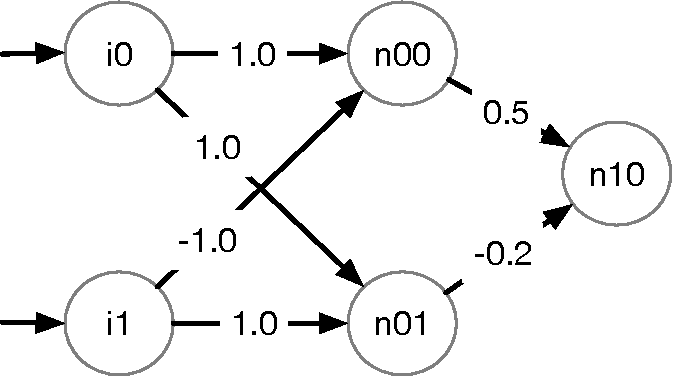
\includegraphics[width=0.6\linewidth]{reluplexA.pdf}
        \caption{A DNN example}\label{fig:reluplex}
    \end{minipage}
    \hfill
    \begin{minipage}{0.50\linewidth}
        \centering
        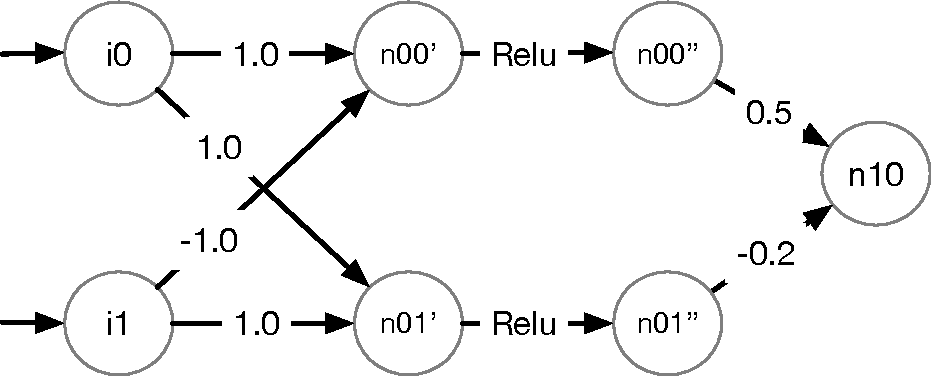
\includegraphics[width=0.9\linewidth]{reluplexB.pdf}
        \caption{Separating nodes to represent RELU}\label{fig:reluplexB}
    \end{minipage}
  \end{figure}

  %TODO: should use our current example, per haps for disproving property.


  \begin{example}\label{ex:reluplex}

  We use the DNN in Fig.~\ref{fig:reluplex} to demonstrate \reluplex{}. Assume we want to check that the DNN has the property
\begin{equation}\label{eq:prop1}
  (0 \le i_0 \le 0.5 \land -2 \le i_1 \le -1) \implies ( n_{10}< 0 \lor n_{10} > 0.5).
\end{equation}
That is, when the inputs $i_0, i_1$ fall within certain ranges, then the result $n_{10}$ has certain values.
As mentioned in~\ref{sec:satisfiability-and-activation-pattern-search}, we turn this into a satisfiability problem by negating the property and checking if the negation is unsatisfiable.
In this case, we want to check if the negation of ~\autoref{eq:prop1} is \unsat{}:
\begin{equation}\label{eq:negprop1}
    ( 0 \le i_0 \le 0.5 \land -2 \le i_1 \le -1) \land 0 \le n_{10} \le 0.5.
  \end{equation}

If~\autoref{eq:negprop1} is \unsat{}, then the DNN satisfies the property in~\autoref{eq:prop1}---there exists no assignment of the inputs $i_0, i_1$ such that the output $n_{10}$ is within the range $[0, 0.5]$. Otherwise, the DNN does not have the property and we can return a counterexample.


\paragraph{Problem Encoding}  A DNN can be encoded as a conjunctions of constraints.  The ReLU node $v$ can be encoded as a pair of variables $v'$ and $v''$, where $v'$ is used to connect the nodes of previous layers to $v$, and $v''$ is used to connect $v$ to the next layer.

For example, in~\autoref{fig:reluplex}, the ReLU node $n00=\max(i0 -1i1,0)$ is encoded using two variables $n00'=i0 -1i1$ and $n00''=\max(n00',0)$.  The DNN in\autoref{fig:reluplexB} shows the network in~\autoref{fig:reluplex} with additional nodes representing ReLU encoding.



The first step to use Repluplex is to encode the constraints representing the DNN and the problem into a format that Reluplex accepts.
The DNN in~\autoref{fig:reluplex} can be encoded as a conjunction of equalities:

\begin{gather*}%\label{eq:reluplex1}
    n00' = i_0 - i_1,\quad n00'' = \max(n00',0),\\
    n01' = i_0 + i_1, \quad n01'' = \max(n01',0),\\
    n_{10} = 0.5n00'' - 0.2n01''
\end{gather*}

\paragraph{Basic Variables} We also introduce three new \emph{basic} (auxilliary or slack) variables to store the relationships of the DNN's constraints:
\begin{gather}
  a_1 = i_0 - v^b_{12} - n00'\label{eq:reluplex2a},\\
  a_2 = i_0 + v^b_{12} - n01'\label{eq:reluplex2b},\\
  a_3 = 0.5n00'' -0.2 n01'' - n_{10}\label{eq:reluplex2c}
\end{gather}

In simplex terminology, a basic variable is a variable that is used to represent the relationship between other variables in the constraints. For example, $a_1$ represents the difference between $i_0$, $v^b_{12}$, and $n00'$. The basic variables are used to maintain the relationships between the variables in the constraints and are updated during the search process.

In contrast, a \emph{non-basic} variable is a variable that is not used to represent the relationship between other variables in the constraints. For example, $i_0$ and $i_1$ are non-basic because they are not used to represent the relationship between other variables in the constraints. Non-basic variables are typically the input variables of the DNN.

\paragraph{Iteration} \reluplex{} first assigns 0 to all \tvn{basic?} variables in the constraints in~\autoref{eq:reluplex2a}--~\autoref{eq:reluplex2c}.  This assignment---essentially an initial guess---would likely cause issues such as variables violating their bounds.  \reluplex{} works by iteratively fixing these invalid values until it finds a feasible assignment (and returns \texttt{sat}) or cannot do so (and returns \texttt{unsat}).

This iterative updating process can be demonstrated through a sequence of configuration updates over the variables.
~\autoref{tab:reluplex1} shows the initial configuration with all values assigned to 0.
Observe that the lower and upper bounds of the inputs $i_0, i_1$ and output $n_{10}$ are specified in the property in ~\autoref{eq:negprop1}, the lower bounds of $v_f$'s representing ReLU are 0, and the other hidden variables are unbounded.

\begin{table}[h]
    \centering
\begin{tabular}{ccccccccccc}
     & $i_0$ & $i_1$ & $n00'$ & $n00''$ & $n01'$ & $n01''$ & $n_{10}$ &$a_1$&$a_2$&$a_3$ \\
    \midrule
    LB & 0 & -2 & $-\infty$&0&$-\infty$& 0 & 0 & 0 & 0 &0\\
    Val& 0 & 0 & 0 & 0 & 0 & 0 & 0 & 0 & 0 & 0\\
    UP & 0.5 & -1 &$\infty$&$\infty$&$\infty$&$\infty$&0.5& 0 & 0 & 0
\end{tabular}
\caption{Configuration \#1}\label{tab:reluplex1}
\end{table}

\autoref{tab:reluplex1} shows that $i_1$ is out-of-bounds because $0 \notin [-2,-1]$. To fix $i_1$, which is non-basic, Reluplex simply updates it to a valid value, e.g., $i_1 \texttt{+=} -1.0 = -1.0$, which means adding -1.0 to the current value of $i_1$ and thus having $i_1= -1.0$.
Now, because $a_1, a_2$ depend on $i_1$ as shown in~\autoref{eq:reluplex2a} and~\autoref{eq:reluplex2b}, respectively, this update to $i_1$ also changes $a_1,a_2$:
    \begin{align*}
        a_1 ~+=~ 1.0 = 1.0   &~\text{because}~ a_1=i_0 - i_1 - n00', \\
        a_2 ~+=~ -1.0 = -1.0  & ~\text{because}~ a_2=i_0 + i_1 - n01'.\\
    \end{align*}



\autoref{tab:reluplex2} shows the new configuration.
\autoref{tab:reluplex2} also shows $a_1, a_2$ violate their bounds and need to be fixed. Assume Reluplex picks $a_1$. To fix $a_1$, which is a basic variable, Reluplex pivots (swaps) it with one of the variables it depends on as shown in the constraint $ a_1 = i_0 - v^b_{12} - n00'$ in~\autoref{eq:reluplex2a}. Assume Reluplex pivots $a_1$ with $n00'$, we get
\begin{equation}\label{eq:reluplex5}
n00' = i_0 - v^b_{12} - a_1.
\end{equation}


\begin{table}[h]
    \centering
\begin{tabular}{ccccccccccc}
     & $i_0$ & $i_1$ & $n00'$ & $n00''$ & $n01'$ & $n01''$ & $n_{10}$ &$a_1$&$a_2$&$a_3$ \\
    \midrule
    LB & 0 & -2 & $-\infty$&0&$-\infty$& 0 & 0 & 0 & 0 &0\\
    Val& 0 & \textbf{-1} & 0 & 0 & 0 & 0 & 0 & \textbf{1} & \textbf{-1} & 0\\
    UP & 0.5 & -1 &$\infty$&$\infty$&$\infty$&$\infty$&0.5& 0 & 0 & 0\\\
\end{tabular}
\caption{Configuration \#2}\label{tab:reluplex2}
\end{table}


Reluplex now updates the non-basic $a_1$ to 0 ($a_1 \text{+=} -1.0 = 0$). This also changes $n00'$  to 1.0 ($n00'+=1.0 = 1.0)$ because $n00'$ depends on $a_1$ as shown in~\autoref{eq:reluplex5}.

\begin{table}[h]
    \centering
\begin{tabular}{ccccccccccc}
     & $i_0$ & $i_1$ & $n00'$ & $n00''$ & $n01'$ & $n01''$ & $n_{10}$ &$a_1$&$a_2$&$a_3$ \\
    \midrule
    LB & 0 & -2 & $-\infty$&0&$-\infty$& 0 & 0 & 0 & 0 &0\\
    Val& 0 & -1 & \textbf{1} & 0 & 0 & 0 & 0 & \textbf{0} & -1 & 0\\
    UP & 0.5 & -1 &$\infty$&$\infty$&$\infty$&$\infty$&0.5& 0 & 0 & 0\\\
\end{tabular}
\caption{Configuration \#3}\label{tab:reluplex3}
\end{table}

~\autoref{tab:reluplex3} shows the new configuration. ~\autoref{tab:reluplex3} also shows the basic variable $a_2$ is out-of-bound.  To fix it, Reluplex pivots $a_2$ with a variable it depends on as shown in the constraint $a_2 = i_0 + v^b_{12} - n01'$ in Eq~\ref{eq:reluplex2b}.  Assume Reluplex pivots $a_2$ with $n01'$, we get
\begin{equation}\label{eq:reluplex6}
  n01' = i_0 + v^b_{12} - a_2
\end{equation}
Now $a_2$ becomes non-basic and is updated to 0 through $a_2+= 1.0 = 0$. As $n01'$ depends on $a_1$ as shown in ~\autoref{eq:reluplex6}, we make the change $n01' ~\texttt{-=}~1.0 = -1.0$.


\begin{table}[h]
    \centering
\begin{tabular}{ccccccccccc}
     & $i_0$ & $i_1$ & $n00'$ & $n00''$ & $n01'$ & $n01''$ & $n_{10}$ &$a_1$&$a_2$&$a_3$ \\
    \midrule
    LB & 0 & -2 & $-\infty$&0&$-\infty$& 0 & 0 & 0 & 0 &0\\
    Val& 0 & -1 & 1 & 0 & \textbf{-1} & 0 & 0 & 0 & \textbf{0} & 0\\
    UP & 0.5 & -1 &$\infty$&$\infty$&$\infty$&$\infty$&0.5& 0 & 0 & 0\\\
\end{tabular}
\caption{Configuration \#4}\label{tab:reluplex4}
\end{table}

~\autoref{tab:reluplex4} shows the new configuration.
At this point, we no longer have out-of-bound variables, but have inconsistent values for the pair of RELU variables $n00', n00''$. This is because $n00'' = \max(n00',0)$ but  we have $n00'=1$ thus $\max(1,0)=1$, which is not $n00''=0$.  Thus, Reluplex needs to fix either $n00''$ or $n00'$.

Assume Reluplex picks $n00''$. Because $n00''$ is non-basic, we simply update it, i.e.,  $n00'' = \text{+} 1 = 1$.  As $a_3$ depends on $n01''$, i.e., $ a_3 = 0.5n00'' -0.2 n01'' - n_{10}$, Reluplex also makes the change $a_3+= 0.5\times 1.0=0.5$.



\begin{table}[h]
    \centering
\begin{tabular}{ccccccccccc}
     & $i_0$ & $i_1$ & $n00'$ & $n00''$ & $n01'$ & $n01''$ & $n_{10}$ &$a_1$&$a_2$&$a_3$ \\
    \midrule
    LB & 0 & -2 & $-\infty$&0&$-\infty$& 0 & 0 & 0 & 0 &0\\
    Val& 0 & -1 & 1 & \textbf{1} & -1 & 0 & 0 & 0 & 0 & \textbf{0.5}\\
    UP & 0.5 & -1 &$\infty$&$\infty$&$\infty$&$\infty$&0.5& 0 & 0 & 0\\\
\end{tabular}
\caption{Configuration \#5}\label{tab:reluplex5}
\end{table}

~\autoref{tab:reluplex5} shows the new configuration.
In the new configuration, $a_3$ is out-of-bound. To fix this basic variable, we pivot $a_3$ with one of the variables $n00'', n01'', n_{10}$ because of the constraint $a_3 = 0.5n00'' -0.2 n01'' - n_{10}$ in ~\autoref{eq:reluplex2c}. Assume we pivot $a_3$ with $n_{10}$, we get
\begin{equation}\label{eq:reluplex7}
  n_{10} = 0.5n00'' -0.2 n01'' - a_3
\end{equation}

Now, $a_3$ becomes non-basic and we update it to 0 through $a_3+=-0.5=0$.  As $n_{10}$ depends on $a_3$ as shown in Eq~\ref{eq:reluplex7}, we make the change $n_{10} += 0.5=0.5$.

\begin{table}[h]
    \centering
\begin{tabular}{ccccccccccc}
     & $i_0$ & $i_1$ & $n00'$ & $n00''$ & $n01'$ & $n01''$ & $n_{10}$ &$a_1$&$a_2$&$a_3$ \\
    \midrule
    LB & 0 & -2 & $-\infty$&0&$-\infty$& 0 & 0 & 0 & 0 &0\\
    Val& 0 & -1 & 1 & \textbf{1} & -1 & 0 & \textbf{0.5} & 0 & 0 & \textbf{0}\\
    UP & 0.5 & -1 &$\infty$&$\infty$&$\infty$&$\infty$&0.5& 0 & 0 & 0\\\
\end{tabular}
\caption{Configuration \#6}\label{tab:reluplex6}
\end{table}

~\autoref{tab:reluplex6} shows the new configuration.
At this point, Reluplex no longer has any out-of-bound or inconsinstent values, and thus stops and returns \sat{} with the values in the \textbf{Val} row in ~\autoref{tab:reluplex6} as the satisfying assignment for the formula in Eq~\ref{eq:negprop1}.

Thus, in this example, we conclude that property in~\autoref{eq:prop1} is \emph{not valid} for the DNN in~\autoref{fig:reluplex} because for the inputs $i_0=0,v_{-12}=-1$, the DNN gives the output $n_{10}=0.5$, which violates the property in~\autoref{eq:prop1}.
\end{example}

\section{Excercises}
\begin{exercise}
Consider the DNN in~\autoref{fig:reluplex} and the property in~\autoref{eq:prop1}.  Use \reluplex{} to verify the property.  If you find a counterexample, provide it.  You will need to provide all the steps in the \reluplex{} algorithm, e.g., DNN encoding, basic variable encoding, and the \reluplex{} search through a series of configurations as shown in~\autoref{ex:reluplex}.

\end{exercise}


\chapter{GPU and Multicore Parallelism}


\part{Survey of DNN Verification Tools}

\chapter{Popular Techniques and Tools}




\part{Advanced Topics\label{part:advanced-topics}}




\chapter{Proof Generation and Checking}\label{chapter:proof-gen-check}

%Advances in DNN verification have made it possible to reason about the safety and robustness of complex DNNs. 
As DNN tools become more complex (e.g., SOTA tools have 20K LoCs), they are more prone to bugs. VNN-COMP'23~\cite{brix2023fourth} showed that 3 of the top 7 participants produced unsound results by claiming unsafe DNNs are safe, i.e., they produce \unsat{} on problems that are actually \sat{}. This is a serious issue, as it can lead to unsafe DNNs being deployed in safety-critical applications, such as autonomous driving and medical diagnosis.

While checking counterexamples is relatively straightforward (we can just evaluate the DNN on the input), checking \unsat{} results---proving no counterexample exists---is far more challenging. This would require verifiers to track their decision steps, which are often complex and large. %Moreover, there are many verification approaches (e.g., branch and bound, conflict-driven learning, abstraction and refinement), making it difficult to standardize and compare results across different tools.
%This is unlike SAT solving, where most tools adopt the standard DPLL framework and thus allows for unified techniques in proof generation and checking (e.g., the DRAT family of algorithms for UNSAT proofs).

\section{Proof Generation}\label{sec:proofgen}

% To successfully deploy DNN verification tools in safety-critical applications, it is essential to provide guarantees that the verification results are correct, i.e., it won't claim an unsafe DNN as safe. One way to achieve this is to generate proofs of the verification results, i.e., a sequence of logical steps that demonstrates the validity of the verification result.
% Ideally, the proof generation process should be automated and integrated into the verification tool, so that the proof can be generated and checked automatically. The challenge is that there are many different DNN verification techniques, each with its own decision-making process, making it difficult to standardize proof generation across different tools. 



A proof of satisfiability (sat) is an input that violates the property, i.e., a counterexample.  We can easily  check such a counterexample $c$ by evaluating $\phi(c,N(c))$ (i.e., running the DNN on the counterexample).
In fact, VNN-COMPs already requires competing DNN verification tools to return counterexamples demonstrating satisfiability.  

In contrast, the proof of an unsatisfiability result (which explains why \emph{no possible inputs} can violate the property) is inherently more complex to generate (\autoref{sec:proofgen}), requires a more sophisticated encoding (\autoref{sec:prooflang}), and an efficient checking algorithm (\autoref{sec:proofchecking}). We are mainly interested in \unsat{} proofs.


\begin{algorithm}[t]
    \footnotesize
  
    \Input{DNN $\mathcal{N}$, property $\phi_{in} \Rightarrow \phi_{out}$}
    \Output{($\unsat, \prooftree$) if property is valid, otherwise ($\sat, \counterexample$)}
    \BlankLine


    $\problems \leftarrow \{ \emptyset \}$ \tcp{initialize verification problems}\label{line:activation} 
    $\prooftree \gets \{ ~ \}$ \tcp{initialize proof tree}\label{line:prooftree}
    
    \While(\tcp*[h]{main loop}){$\problems$}{\label{line:dpllstart}
        % \tcp{$\sigma_i$ is the activation pattern of problem $i$-th}
        $\sigma_i \gets \Select(\problems)$ \tcp{process problem $i$-th}
        % \Parfor(\tcp*[h]{process in parallel}){$\sigma_i ~\In~ \problems$}{ \label{line:parfor}
            \If{\Deduce{$\mathcal{N}, \phi_{in}, \phi_{out}, \sigma_i$}}{\label{line:deduce}
                $(\counterexample, v_i) \leftarrow \Decide(\mathcal{N}, \phi_{in}, \phi_{out}, \sigma_i)$ \\ \label{line:decide}
                \If(\tcp*[h]{found a valid counter-example}){$\counterexample$}{
                    \Return{$(\sat, \counterexample)$} 
                }
                \tcp{create new activation patterns}
                $\problems \leftarrow \problems \cup \{ \sigma_i \land v_i ~;~ \sigma_i \land \overline{v_i} \}$ \;
            }
            \Else(\tcp*[h]{detect a conflict}){
                % $\clauses \leftarrow \clauses \cup \AnalyzeConflict(\igraph_i)$ \\ \label{line:analyze_conflict}
                $\prooftree \leftarrow \prooftree \cup \{ \sigma_i \}$ \tcp{build proof tree} \label{line:record_proof}
            }
        % }
        % \If(\tcp*[h]{no more problems}){$\isEmpty(\problems)$}{
        % }
        
    }\label{line:dpllend}
    \Return{$(\unsat, \prooftree)$}
    
    \caption{The \proofgen{} DNN verification with proof generation.}\label{alg:bab-proof}
\end{algorithm}



%\emph{Branch-and-bound} (BaB) is a common approach to DNN verification and used by major DNN verification tools including~\cite{bunel2020branch,wang2021beta,ferrari2022complete,duong2024harnessing,duong2023dpllt,ovalbab}.
%In BaB algorithms, ``branch'' means splitting the problem into smaller subproblems (like a search tree), and ``bound'' means computing the upper and lower bounds, using abstraction, of the problem to prune the search space. 



%Among modern DNN verification techniques, only the simplex-based approach attempts to generate proofs~\cite{desmartin2023towards,barbosa2023generating}. However, generating a proof for simplex-based approaches is non-trivial and incurs a significant overhead during the verification process~\cite{desmartin2023towards,barbosa2023generating}.

%Recently, an approach based on the DPLL(T) algorithm in SAT/SMT solving has shown much promise~\cite{duong2023dpllt}. For example, in its debut year, the DPLL(T)-based \neuralsat{} DNN verifier~\cite{duong2023dpllt} won the New Comer Award at VNN-COMP'23~\cite{brix2023fourth} and outperformed other state-of-the-art DNN verification tools, especially for very large networks~\cite{duong2024harnessing}. More importantly, DPLL(T) approach maintains \emph{implication graph}, an internal data structure to keep track of assignments, which essentially represent a  proof of the verification result. In other words, proofs are a built-in feature of DPLL(T) approach, and thus can be generated with minimal (in fact, \emph{zero}) overhead.

\subsection{Proof Generation for Branch and Bound (BaB) Algorithms}\label{sec:proogen}

As mentioned in~\autoref{chap:bab}, major DNN verification techniques share the common ``branch and bound'' (BaB) search algorithm. The BaB structure, shown in~ \autoref{alg:bab}, splits the problem into smaller subproblems and use abstraction to compute bounds to prune the search space. This commonality allows us to bring proof generation capabilities with minimal overhead to existing DNN verification tools.

\autoref{alg:bab-proof} extends~\autoref{alg:bab} to show \proofgen, a BaB-based DNN verification algorithm with proof generation capability. The key idea is to introduce a proof tree (\autoref{line:prooftree}) and recording the branching decisions to the proof tree (\autoref{line:record_proof}).
The proof tree is a binary tree structure, where each node represents a neuron and its left and right edges represent its activation decision (active or inactive).
At the end of the verification process, the proof tree is returned as the proof of \unsat{} result.



% \bab{}, a reference architecture~\cite{nakagawa2014consolidating} 
% for modern DNN verifiers that we use to illustrate our observations.  
% \bab{} takes as input a ReLU-based DNN $\mathcal{N}$ and a formulae $\phi_{in}\Rightarrow \phi_{out}$ representing the property of interest.

%\bab{} iterates between two components: \texttt{Decide} (branching, \autoref{line:decide}), which decides (assigns) an activation status value for a neuron, and \texttt{Deduce} (bounding, \autoref{line:deduce}), which checks the feasibility of the current activation pattern. 
%To add proof generation capability, \bab{} is instrumented with a proof tree (\texttt{proof}) variable (\autoref{line:prooftree}) to record these branching decisions. The proof is represented as a binary tree structure, where each node represents a neuron and its left and right edges represent its activation decision (active or inactive). %The proof tree is then used to generate a proof in the \prooflang{} format (\autoref{sec:proof-format}).




\begin{figure}[t]
    \begin{minipage}[b]{\linewidth}
        \centering
        \begin{minipage}[t]{0.48\textwidth}
            \centering  
            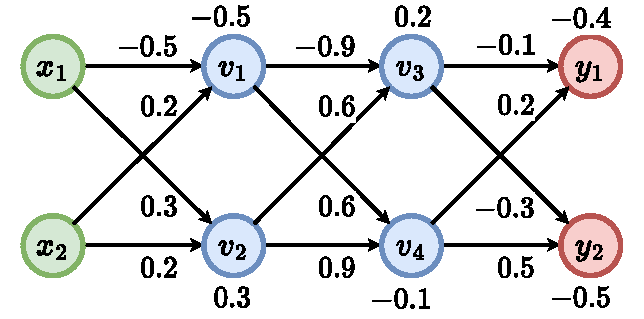
\includegraphics[width=\linewidth]{figure/proof_net.pdf}
            \caption*{(a)}
        \end{minipage}
        \begin{minipage}[t]{0.48\textwidth}
            \centering
            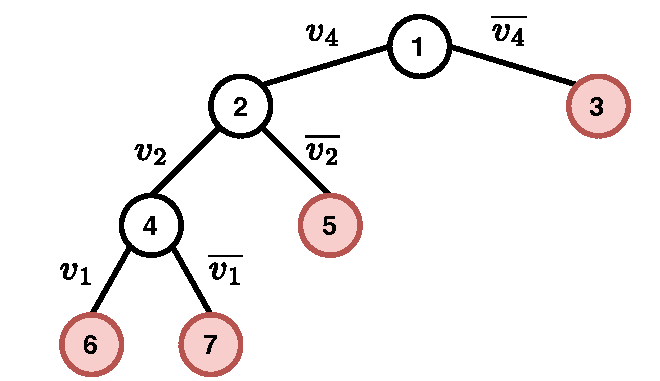
\includegraphics[width=\linewidth]{figure/proof_tree.pdf}
            \caption*{(b)}
        \end{minipage}
        \caption{(a) A simple DNN  (a redrawn of~\autoref{fig:example1}), and (b) A proof tree produced verifying the property $(x_1, x_2) \in [-2.0, 2.0] \times [-1.0, 1,0] \Rightarrow (y_1 > y_2)$.}
        \label{fig:example}
    \end{minipage}
\end{figure}
%White nodes correspond to branching nodes where \neuralsat{} makes decisions to split ReLU neurons.

\paragraph{Example} We reuse the example in~\autoref{chap:bab} to illustrate \proofgen{}. Recall the goal is to verify that the DNN in \autoref{fig:example}(a) (a redraw of~\autoref{fig:example1}) has the property $(x_1, x_2) \in [-2.0, 2.0] \times [-1.0, 1,0] \Rightarrow (y_1 > y_2)$. \proofgen{} generates the proof tree in \autoref{fig:example}(b) to show unsatisfiability, i.e., the property is valid.

First, \proofgen{} initializes the activation pattern set \functiontextformat{ActPatterns} with an empty activation pattern $\emptyset$. Then \proofgen{} enters a loop (\autoref{line:dpllstart}-\autoref{line:dpllend}) to search for a satisfying assignment or a proof of unsatisfiability. In the first iteration, \proofgen{} selects the only available activation pattern $\emptyset \in \functiontextformat{ActPatterns}$. 
It calls~\functiontextformat{Deduce} to check the feasibility of the problem based on the current activation pattern. \functiontextformat{Deduce} uses abstraction to approximate that from the input constraints the output values are feasible for the given network. 
Since \functiontextformat{Deduce} cannot decide infeasibility, \proofgen{} randomly selects a neuron to split (\functiontextformat{Decide}). Let us assume that it chooses $v_4$ to split, which essentially means the problem is split into two independent subproblems: one with $v_4$ active and the other with $v_4$ inactive.
\proofgen{} then adds $v_4$ and $\overline{v_4}$ to \functiontextformat{ActPatterns}.

In the second iteration, \proofgen{} has two subproblems (that can be processed in parallel). For the first subproblem with $v_4$, \functiontextformat{Deduce} cannot decide infeasibility, so it selects $v_2$ to split. It then conjoins $v_4$ with $v_2$ and then with $\overline{v_2}$ and adds both conjuncts to \texttt{ActPatterns}. 
For the second subproblem with $\overline{v_4}$ inactive, \functiontextformat{Deduce} determines that the problem is unsatisfiable and \proofgen{} saves the node $v_4$ to the proof tree, as node 3, to indicate one unsatisfiable pattern, i.e., whenever the network has $v_4$ being inactive, the problem is unsatisfiable.

In the third iteration, \proofgen{} has two subproblems for $v_4 \land v_2$ and $v_4 \land \overline{v_2}$. For the first subproblem, \functiontextformat{Deduce} cannot decide infeasibility, so it selects $v_1$ to split. It then conjoins $v_1$ and then $\overline{v_1}$ to the current activation pattern and adds them to \functiontextformat{ActPatterns}. For the second subproblem, \functiontextformat{Deduce} determines that the problem is unsatisfiable and \proofgen{} saves the node $v_4 \land \overline{v_2}$ to the proof tree, as node 5.

In the fourth iteration, \proofgen{} has two subproblems for $v_4 \land v_2 \land v_1$ and $v_4 \land v_2 \land \overline{v_1}$. Both subproblems are determined to be unsatisfiable, and \proofgen{} saves them to the proof tree as nodes 6 and 7, respectively.

Finally, \proofgen{} has an empty \texttt{ActPatterns}, stops the search, and returns \texttt{unsat} and the proof tree. 

\section{Proof Language}\label{sec:prooflang}


\newcommand{\lra}[1]{
    \textcolor{green!40!black}{\langle} 
    \textit{\textcolor{green!40!black}{#1}} 
    \textcolor{green!40!black}{\rangle}
}

\begin{figure}
{\small
\begin{align*}
    \lra{proof}         &::= \lra{declarations} \ \lra{assertions} \\
    \lra{declarations}  &::= \lra{declaration} \ | \ \lra{declaration} \ \lra{declarations} \\
    \lra{declaration}   &::= (\textbf{declare-const} \ \lra{input-vars} \ \textbf{Real}) \\
                        & \quad ~| \ (\textbf{declare-const} \ \lra{output-vars} \ \textbf{Real}) \\
                        & \quad ~| \ (\textbf{declare-pwl} \ \lra{hidden-vars} \ \lra{activation}) \\
    \lra{input-vars}    &::= \lra{input-var} \ | \ \lra{input-var} \ \lra{input-vars} \\
    \lra{output-vars}    &::= \lra{output-var} \ | \ \lra{output-var} \ \lra{output-vars} \\
    \lra{hidden-vars}    &::= \lra{hidden-var} \ | \ \lra{hidden-var} \ \lra{hidden-vars} \\
    \lra{activation}    &::= ~\text{ReLU} \ | \ \text{Leaky ReLU} \ | \ \ldots \\
    \lra{assertions}    &::= \lra{assertion} \ | \ \lra{assertion} \ \lra{assertions} \\
    \lra{assertion}     &::= (\textbf{assert} \ \lra{formula}) \\
    \lra{formula}       &::= (\lra{operator} \ \lra{term} \ \lra{term}) \\
                        & \quad ~| \ (\textbf{and} \ \lra{formula}+) \ | \ (\textbf{or} \ \lra{formula}+) \\
                        % & \quad ~| \ (\textbf{and} \ \lra{formula} \ \lra{formula}) \\
                        % & \quad ~| \ (\textbf{or} \ \lra{formula}+) \\
                        % & \quad ~| \ (\textbf{or} \ \lra{formula} \ \lra{formula}) \\
    \lra{term}          &::= \lra{input-var} \ | \ \lra{output-var} \\ 
                        & \quad ~| \ \lra{hidden-var} \ | \ \lra{constant} \\
    \lra{operator}      &::= ~ < \ | \ \leq \ | \ > \ | \ \geq \\
    \lra{input-var}     &::= ~\text{X\_}\lra{constant} \\
    \lra{output-var}    &::= ~\text{Y\_}\lra{constant} \\
    \lra{hidden-var}    &::= ~\text{N\_}\lra{constant} \\
    \lra{constant}      &::= ~\textbf{Int} \ | \ \textbf{Real}
\end{align*}
}
\caption{The \prooflang{} proof language.}\label{fig:grammar}
\end{figure}

In~\autoref{sec:proofgen} we have shown that the BaB class of DNN verification techniques  can generate a binary tree that represents a proof of unsatisfiability.
Rather than record such proofs in an verifier-specific format, it is more desirable to have a standard format
that is human-readable, is compact, can be efficiently generated by verification tools, and can
be efficiently and independently processed by proof checkers.  

To meet this goal, we introduce \prooflang{}, a proof language to specify DNN proofs.
This language is inspired by the SMTLIB format~\cite{barrett2010smt} used for SMT solving, which has also been adopted by the  VNNLIB language~\cite{vnnlib} to specify DNNs and their properties for  verification.

%accepted by our proof check algorithm (\autoref{sec:proof-checker}

\autoref{fig:grammar} outlines the \prooflang{} syntax and grammar, represented as production rules. 
A proof is composed of \textit{declarations} and \textit{assertions}. Declarations define the variables and their types within the proof. Specifically, \textit{input variables} (prefixed with \functiontextformat{X}) and \textit{output variables} (prefixed with \functiontextformat{Y}) are declared as real numbers, representing the inputs and outputs of the neural network, respectively. Additionally, \textit{hidden variables} are declared with specific piece-wise linear (PWL) activation functions, such as ReLU or Leaky ReLU. These hidden variables correspond to the internal nodes of the neural network that process the input data through various activation functions.

Assertions are logical statements that specify the conditions or properties that must hold within the proof. Assertions over input variables are \emph{preconditions} and those over output variables are \emph{post-conditions}. Each assertion is composed of a \textit{formula}, which can involve terms and logical operators. Formulas include simple comparisons between terms (e.g., less than, greater than) or more complex logical combinations using \functiontextformat{and} and \functiontextformat{or} operators. The terms used in these formulas can be input variables, output variables, hidden variables, or constants.

\begin{figure}
\begin{lstlisting}[style=SMTLIB-style, language=SMTLIB, basicstyle=\ttfamily\scriptsize]
; Declare variables
(declare-const X_0 X_1 Real)
(declare-const Y_0 Y_1 Real)
(declare-pwl N_1 N_2 N_3 N_4 ReLU)

; Input constraints
(assert (>= X_0 -2.0))
(assert (<= X_0  2.0))
(assert (>= X_1 -1.0))
(assert (<= X_1  1.0))

; Output constraints
(assert (<= Y_0 Y_1)) 

; Hidden constraints
(assert (or 
    (and (<  N_4 0))
    (and (<  N_2 0) (>= N_4 0))
    (and (>= N_2 0) (>= N_1 0) (>= N_4 0))
    (and (>= N_2 0) (<  N_1 0) (>= N_4 0))))
\end{lstlisting}
\caption{\prooflang{} example format of the proof tree in \autoref{fig:example}b. 
%\tvn{seems to take too much space. Could we put multiple statements in a line?}\hd{is it compact enough?}\tvn{yep. thanks}
}
\label{fig:proof_example}
\end{figure}

%\autoref{fig:proof_example} shows an example of a proof in \prooflang{} using the network in \autoref{fig:example}a. 

The \texttt{declare-*} statements declare input, output, and hidden variables, while the \texttt{assert} statements specify the constraints on these variables (i.e., the pre and postcondition of the desired property).
The hidden constraints represent the activation patterns of the hidden neurons in the network (i.e., the proof tree). Each \texttt{and} statement represents a tree path that represents an activation pattern. 



\begin{example} 
    The proof in \autoref{fig:proof_example} corresponds to the proof tree in \autoref{fig:example}b. The statement \texttt{(and (< N\_4 0))} corresponds to the rightmost path of the tree with $\overline{v_4}$ decision (leaf 3).  The statement \texttt{(and (< N\_2 0) (>= N\_4 0))} corresponds to the path with $v_4 \land \overline{v_2}$ (leaf 5). 
\end{example}

The \prooflang{} language is intentionally designed to (a) not explicitly include weights/bias terms to minimize size of the proof structure, and (b) explicitly reflect a DNF structure to enable easy parallelization.
The DNN weight and bias terms are readily available in the standard ONNX~\cite{onnx} format, which is typically used to represent the DNN input to a \proofgen{}-based DNN verification tool and can be accessed by any \prooflang{} checker like the one described next in~\autoref{sec:proofchecking}.


\section{Proof Checker}\label{sec:proofchecking}
Finally, we need to check that the generated proof is correct and that the original NN verification problem is indeed unsatisfiable. The checker must be efficient to handle large proofs and trusted of its results (if it verifies the proof, then the original NNV problem is proved).


To achieve this, we present \proofcheck{}, a proof checker for \prooflang{} proofs.
\proofcheck{} is verifier-independent and support \prooflang{} proofs generated by different verification tools. \proofcheck{} also has several optimizations to handle large proofs efficiently.

\subsection{The Core \proofcheck{} Algorithm}


The goal of \proofcheck{} is to verify that the \prooflang{} tree generated by a DNN verification tool is correct (i.e., the proof tree is a proof of unsatisfiability of the DNN verification problem).
\proofcheck{} thus must verify that the constraint represented by each \emph{leaf} node in the proof tree is unsatisfiable. To check each node, \proofcheck{} forms an MILP problem (\autoref{sec:milp}) consisting of the constraint in \autoref{eq:prob} (the DNN, the input condition, and the negation of the output) with the constraints representing the activation pattern encoded by the tree path to the leaf node. \proofcheck{} then invokes an LP solver to check that the MILP problem is infeasible, which indicates unsatisfiability of the leaf node. 

\begin{algorithm}[t]
    \footnotesize

    \Input{DNN $\mathcal{N}$, property $\phi_{in} \Rightarrow \phi_{out}$, $\prooftree$}
    \Output{\certified if proof is valid, otherwise \uncertified}
    \BlankLine

    \If{$\neg$ \RepOK(\prooftree)}{
        \RaiseError{Invalid proof tree}
    }

    \tcp{initialize MILP model with inputs}
    $\model \leftarrow \CreateStabilizedMILP(\mathcal{N}, \phi_{in}, \phi_{out})$ \label{line:build_model}

    
    $\leaf \gets \mynull$ \tcp{initialize current processing node}
    
    \While{$\prooftree$}{\label{line:proof_loop}
        
        % \tcp{Get $k$ leaf nodes from $\prooftree$}
        % $[\leaf_1, ..., \leaf_k] \gets \GetLeafNodes(\prooftree, k)$ \\ \label{line:get_leaf}
        $\leaf \gets \Select(\prooftree, \leaf)$ \tcp{get next node to check} \label{line:select} \label{line:get_leaf}

        % \tcp{Process $k$ nodes in parallel}
        % \Parfor{$\leaf_i ~\In~ [\leaf_1, ..., \leaf_k]$}{ \label{line:parfor}
        
        $\model \gets \AddConstrs(\model, \leaf)$  \tcp{add constraints} \label{line:add_proof_leaf_constrs}
        
        % $\minimum \gets \Minimize(\model)$ \tcp{} \label{line:optimize1}
        \If{$\Feasible(\model)$}{\label{line:proof_check_objective1}
            \Return{\uncertified} \tcp{cannot certify}
        }
        
        % $\Backtrack(\prooftree, \leaf)$ \tcp{process interior node}
        
        % \While{$\StoppingConditions(\leaf_i)$}{ \label{line:stop_condition}
        %     % \tcp{remove constraints of old $\leaf_i$ }
        %     % $\model \gets \RemoveConstrs(\model, \leaf_i)$  \\
        %     % \tcp{move to $\leaf_i$'s parent}
        %     % $\leaf_i \gets \ShortenSplitConstrs(\leaf_i)$ \\
        %     % \tcp{add constraints of new (looser) $\leaf_i$ }

        %     \tcp{move to $\leaf_i$'s parent}
        %     $\model \gets \Backjump(\leaf_i)$  \\ \label{line:proof_backjump}

        %     \tcp{Prove the new $\leaf_i$}
        %     $\minimum \gets \Minimize(\model)$ \\ \label{line:optimize2}
        %     \If(\tcp*[h]{cannot certify}){$\minimum \le 0$}{
        %         \Break
        %     }
        %     \tcp{if parent is proved, remove its children}
        %     $\prooftree \gets \RemoveLeafNodes(\prooftree, \leaf_i)$ \label{line:proof_prune}
        % }
        }
    % }
    \Return{\certified}

    \caption{\proofcheck{} algorithm.}
    % \Description{}
    \label{fig:algorithm}
\end{algorithm}


\autoref{fig:algorithm} shows a minimal (core)  \proofcheck{} algorithm, which takes as input a DNN $\mathcal{N}$, a property $\phi_{in} \Rightarrow \phi_{out}$, a proof tree $\prooftree$, and returns \certified if the proof tree is valid and \uncertified otherwise. 
\proofcheck{} first checks the validity of the proof tree (\autoref{line:build_model}), i.e., the input must represent a proper \prooflang{} proof tree (\autoref{sec:prooflang}).  
If the proof tree is invalid, \proofcheck{} raises an error.
\proofcheck{} next creates a MILP model (\autoref{line:build_model}) representing the input. % (\autoref{sec:neuron-stabelization}).
\proofcheck{} then enters a loop (\autoref{line:proof_loop}) that selects a (random) leaf node from the proof tree (\autoref{line:select}) and adds its MILP constraint to the model (\autoref{line:add_proof_leaf_constrs}). It then checks the model using an LP solver to determine whether the leaf node is unsatisfiable. If the LP solver returns feasibility, \proofcheck{} returns \uncertified, i.e., it cannot verify the input proof tree. 
\proofcheck{} continues until all leaf nodes are checked and returns \certified, indicating the proof tree is valid.



\begin{example} 
    For the \prooflang{} proof in \autoref{fig:proof_example}, we need to check that the four leaf nodes 3, 5, 6, and 7 of the proof tree in \autoref{fig:example}b are unsatisfiability. Assume \proofcheck{} first selects node 3, it forms the MILP problem for leaf node 3 by conjoining the constraint representing $0.6v_1 + 0.9v_2 - 0.1 \le 0$ (i.e., $\overline{v_4}$) %\tvn{Hai check}\hd{by setting $a_1^{(2)}=0$ representing that $\hat{z}_1^{(2)} \le 0$ (see \autoref{eq:mip}e) or \emph{implicitly} conjoining the inequality $0.6\hat{z}^{(1)}_0 + 0.9\hat{z}^{(1)}_1 - 0.1 \le 0$ (or ${z}_1^{(2)} \le 0$), where $\hat{z}^{(1)}_0$, $\hat{z}^{(1)}_1$ represent the outputs of $v_1$ and $v_2$, respectively.} 
with the constraints in \autoref{eq:prob} representing the input ranges and the DNN with the objective of optimizing the output. \proofcheck{} then invokes an LP solver, which determines that this MILP is infeasible, i.e., leaf node 3 indeed leads to unsatisfiability. \proofcheck{} continues this process for the other three leaf nodes and returns \certified as all leaf nodes are unsatisfiable.
\end{example}

\subsubsection{MILP Formulation}\label{sec:milp-formulation}

\proofcheck{} formulates MILP problems~\cite{tjeng2019evaluating} and check for feasible solutions using off-the-shelf LP solving. Formally, the MILP problem is defined as:
\begin{equation}
    \begin{aligned}
        &\mbox{(a)}\quad z^{(i)} = W^{(i)} \hat{z}^{(i-i)} + b^{(i)};\\
        &\mbox{(b)}\quad y = z^{(L)};  x = \hat{z}^{(0)}; \\
        &\mbox{(c)}\quad \hat{z}_j^{(i)} \ge {z}_j^{(i)}; \hat{z}_j^{(i)} \ge 0; \\
        &\mbox{(d)}\quad a_j^{(i)} \in \{ 0, 1\} ;\\
        &\mbox{(e)}\quad \hat{z}_j^{(i)} \le {a}_j^{(i)} {u}_j^{(i)}; \hat{z}_j^{(i)} \le {z}_j^{(i)} - {l}_j^{(i)}(1 - {a}_j^{(i)}); \\
    \end{aligned}
    \label{eq:mip}
\end{equation}

\noindent where $x$ is input, $y$ is output, and $z^{(i)}$, $\hat{z}^{(i)}$, $W^{(i)}$, and $b^{(i)}$ are the pre-activation, post-activation, weight, and bias vectors for layer $i$, respectively. 
This encodes the semantics of a ReLU-based DNN:  
(a) the affine transformation computing the pre-activation value for a neuron in terms of outputs in the preceding layer;
(b) the inputs and outputs in terms of the adjacent hidden layers;
(c) assertion that post-activation values are non-negative and no less than pre-activation values;
(d) neuron activation status indicator variables that are either 0 or 1; and
(e) constraints on the upper, $u_j^{(i)}$, and lower, $l_j^{(i)}$, bounds of the pre-activation value of the $j$th neuron in the $i$th layer.
Deactivating a neuron, $a_j^{(i)} = 0$, simplifies the first of the (e) constraints to $\hat{z}_j^{(i)} \le 0$, and activating a neuron simplifies the second to $\hat{z}_j^{(i)} \le z_j^{(i)}$, which is consistent with the semantics of $\hat{z}_j^{(i)} = max(z_j^{(i)},0)$.


\subsubsection{Correctness}\label{sec:checker-core-correctness}

 \autoref{fig:algorithm} returns \certified iff the input \prooflang{} proof tree is unsatisfiable. This proof tree encodes a disjunction of constraints, one per tree path, where each constraint represents an activation pattern of the network (the leaf node). The algorithm checks each constraint using LP solving and only returns certified iff every one of them is unsatisfiable.  
%Moreover, while pruning optimization (\autoref{sec:pruning}) in \autoref{fig:algorithm} allows the checker to skip children nodes if the parent node is unsatisfiable, this is still sound because the structure of the proof tree guarantees that the constraints of a child is more restricted its parent, and thus if the parent node is unsatisfiable, the children nodes must also be unsatisfiable. The algorithm  terminates because the proof tree (or the DNF) is finite and the checker will eventually check all nodes.
We note that this correctness argument assumes that the LP solver is correct -- in practice
multiple solvers could be used to guard against errors in that component.  We note that
it is standard for proof checkers to assume the correctness of a small set of external tools, e.g., checkers that use  theorem provers assume the correctness of the underlying prover~\cite{lammich2023grat}.

\subsection{Optimizations}
While the core \proofcheck{} algorithm in \autoref{fig:algorithm} is minimal, it can be inefficicient for large proofs.
\proofcheck{} employs several optimizations to improve its efficiency. These are crucial for checking large proof trees generated by DNN verification tools for challenging problems.


\subsubsection{Neuron Stabilization}\label{sec:neuron-stabelization} 

\begin{algorithm}[t]
    \footnotesize

    \Input{DNN $\mathcal{N}$, property $\phi_{in} \Rightarrow \phi_{out}$, parallel factor $k$}
    \Output{MILP $\model$}
    \BlankLine
    

    $\model \leftarrow \InputMILP(\phi_{in})$  \tcp{input property}    \label{line:create_input}

    \tcp{Add MILP constraints for each layer of network}
    \For{$\layer ~\In ~\mathcal{N}$}{
        \If{$\isPiecewiseLinear(\layer)$}{
            \tcp{add constraints \autoref{eq:mip} (c), (d), (e)} 
            $\model \leftarrow \PiecewiseLinearMILP(\layer, \phi_{in}, \phi_{out})$ \\ \label{line:create_pwl_layer}
        }
        \Else(\tcp*[h]{this layer is linear}){
            \tcp{add constraints \autoref{eq:mip} (a), (b)} 
            $\model \leftarrow \LinearMILP(\layer, \phi_{in}, \phi_{out})$ \\ \label{line:create_linear_layer}

            \tcp{estimate upper and lower bounds} 
            $\layerbounds \gets \EstimateBounds(\layer)$ \\ \label{line:estimate_bounds}
            
            \tcp{select unstable neurons to be stabilized} 
            $[v_1, ..., v_k] \leftarrow \GetUnstableNeurons(\layerbounds)$ \\ \label{line:find_unstable}
        
            \tcp{stabilize selected neurons in parallel}
            \Parfor{$v_i ~\In~[v_1, ..., v_k]$}{ \label{line:parallel_stabilize}
                % \tcp{lower is closer to 0 than upper}
                \tcp{optimize lower first}
                \If{$(v_i.lower + v_i.upper) \ge 0$}{
                    $\Maximize(\model, v_i.lower)$ \\ \label{line:maximize1}
                    \If(\tcp*[h]{still unstable}){$v_i.lower < 0$}{
                        $\Minimize(\model, v_i.upper)$ \label{line:minimize1}
                    }
                }
                % \tcp{upper is closer to 0 than lower}
                % \tcp{optimize upper first}
                \Else(\tcp*[h]{optimize upper first}){
                    $\Minimize(\model, v_i.upper)$ \\ \label{line:minimize2}
                    \If(\tcp*[h]{still unstable}){$v_i.upper > 0$}{
                        $\Maximize(\model, v_i.lower)$  \label{line:maximize2}
                    }
                }
            }
        }
    }

    $\model \gets \AddObjective(\model, \phi_{out})$ \tcp{output property}
    
    \Return{$\model$}
    
    % \vspace*{-0.2in}
    \caption{\texttt{CreateStabilizedMILP} procedure.}
    \label{fig:stabilize}
    % \Description{}
\end{algorithm}

A primary challenge in DNN analysis is the presence of large numbers of piecewise-linear constraints (e.g., ReLU) which generate a large number of branches and yield large proof trees. In the MILP formulation, this creates many disjunctions which are hard to solve. To reduce the number of disjunctions, \proofcheck{} uses \emph{neuron stabilization}~\cite{duong2024harnessing}
to determine neurons that are \emph{stable}, either active or inactive, for all inputs defined by the property pre-condition.
For all stable neurons, the disjunctive ReLU constraint is replaced with a linear constraint that represents the neuron's value.   This simplifies the MILP problem.

\proofcheck{} uses the algorithm in \autoref{fig:stabilize} to traverse the DNN and compute stable neurons. The algorithm initializes the MILP model with input constraints (\autoref{line:create_input}) and then iterates over each layer of the network. 
%follows the~\autoref{eq:mip} to create corresponding 
Next, for each layer, it creates constraints (\autoref{line:create_pwl_layer} or \autoref{line:create_linear_layer}) depending on the layer type.
Moreover,  it uses approximation to estimate bounds of neuron values to determine neuron stability (\autoref{line:estimate_bounds}).
Next, it filters unstable neurons (\autoref{line:find_unstable}) and attempt to make them stable by optimizing either their lower ($\Maximize$) or upper ($\Minimize$) bounds.



\subsubsection{Pruning Leaf Nodes}\label{sec:pruning}
%\hd{``Pruning'' sounds better}

Another optimization \proofcheck{} employs is that it does not check child nodes if the parent node is unsatisfiable.
In an \prooflang{} proof tree, a child node adds constraints to the parent (e.g., node 6 adds the constraint of $v_1$ to node 4, which adds the constraint of $v_2$ to node 2 in \autoref{fig:example}b). Thus, if we determine that the constraint of the parent is unsatisfiable, we can skip the child nodes, which must also be unsatisfiable.  

%Simply checking parent nodes would actually increase MILP cost, because they have shorter tree paths and thus have a greater number of disjunctive constraints.

\proofcheck{} uses a backtracking mechanism to check the parent node only when the child nodes are infeasible. Specifically, it starts checking a leaf node $l$. If it determines unsatisfiability it will check the parent $p$ of $l$. If $p$ is unsatisfiable it immediately removes the children of $p$ (more specifically the sibling of $l$). Next it backtracks to the parent of $p$ and repeats until meeting a stopping criteria. This optimization reduces the number of LP problems that need to be solved, making the proof checking process more efficient. 

We implement a backjumping strategy that allows for backtracking multiple levels, $N$, rather than a single level at a time.
A large value of $N$ offers the chance for greater pruning if an unsatisfiable node is found by
backjumping, but such nodes also represent less constrained, and therefore, more complex MILP problems
and are less likely to be unsatisfiable.
The default value in $\proofcheck{}$ is $N=2$ is selected to enable a modest degree of pruning,
while being close enough to a proven unsatisfiable node that it has a reasonable chance of itself being unsatisfiable.
Future work will explore tuning $N$ to a given verification problem.


% \hd{Without X, \proofcheck{} will have to check all the children.}

% \hd{It backjumps when the leave node is proved and X optimization is enabled. 
% We can keep backing up until it cannot prove anymore, however, after N times, each time half the length of an activation pattern, an activation pattern is shortened to $1 / 2^{N}$ (e.g., if $N=2$, after 2 times of backing up, an activation pattern is shortened to 1/4 of its length). 
% This is when the pruned leaves by those proved interiors are getting overlapped (due to parallelization, we backjump on multiple leaves), so more backjumps might not helpful. 
% Instead, we start over with a new iteration with remaining leaves.
% I experienced with $N = \{1, 2, 3, 4, 5\}$ and I settled down $N=2$ for all experiments (fixed N) which seems to be good enough in our experiments. 
% Increasing $N$ does not improve the performances but hurts especially when dealing with CNNs.
% }
% \matt{I think my main point is ``How much of this is important to \proofcheck{}?'' whatever is important needs to be described.  You don't need to describe all of the discarded alternatives.  If we settled on a particular strategy, then define that strategy and say why it works well, e.g., balances cost of failing to prove unsat for parents with ability to prune sub-trees.  Right now we just say "simple backtracking mechanism", but your description makes seem like it is not all that simple.}
% This optimization reduces the number of LP problems that need to be solved, making the proof checking process more efficient.

%. \proofcheck{} thus uses a simple backtracking mechanism to check the parent node only when the child nodes are infeasible. This optimization reduces the number of LP problems that need to be solved, making the proof checking process more efficient.
%However, checking the parent node is more expensive than checking the child nodes (otherwise we can just directly check the root node). \proofcheck{} thus uses a simple backtracking mechanism to check the parent node only when the child nodes are infeasible. This optimization reduces the number of LP problems that need to be solved, making the proof checking process more efficient.

\subsubsection{Parallelization} Finally, the structure of \prooflang{} proof tree is designed to be easily parallelized.  Each tree path is an independent sub-proof and partitions of the tree allow checker to leverage multiprocessing to check large proof trees efficiently. \proofcheck{} uses a parameter $k$ to control the number of leaf nodes to be checked in parallel.

\section{Rounding Errors}\label{sec:rounding-errors}

\tvn{Give concrete examples of rounding errors in VNN-COMP}


% \section{Evaluation}\label{sec:evaluation}  
% Our goals are to understand how checking of \prooflang{}s performs, how it can be optimized, and how robust checking is to
% verification optimizations.
% We focus our evaluation on the following research questions:

% \noindent\mbox{~~}\textbf{RQ1} (\autoref{sec:rq1}): How does \proofcheck{} perform and how does it compare prior work? 

% \noindent\mbox{~~}\textbf{RQ2} (\autoref{sec:rq2}): How does proof checking optimization improve performance?

% \noindent\mbox{~~}\textbf{RQ3} (\autoref{sec:rq3}): How does proof checking performance vary with verification algorithms and optimizations?



% \subsection{Experimental Design}\label{sec:exp_design}
% We describe the selection of benchmarks, baselines, metrics, and treatments used
% to explore the above RQs.

% \ignore{
% \begin{table*}[t]
%     \footnotesize
%     \centering
%     \caption{Benchmark instances. U: \texttt{unsat}, S: \texttt{sat}, ?: \texttt{unknown}.}\label{tab:benchmarks}
%     % \vspace*{-3mm}
%     % \resizebox{\textwidth}{!}{
%     \begin{tabular}{c|ccrr|cc}
%         \toprule
%         % \multirow{2}{*}{\textbf{Benchmarks}} &\multicolumn{3}{c}{\textbf{Networks}}  &\multicolumn{2}{|c}{\textbf{Tasks}}\\
%         % \multirow{2}{*}{\textbf{Benchmarks}} &\multicolumn{2}{c}{\textbf{Networks}} &  \multicolumn{2}{c|}{\textbf{Per Network}} &\multicolumn{2}{c}{\textbf{Tasks}}\\
%         \multirow{2}{*}{\textbf{Benchmarks}} &\multicolumn{4}{c}{\textbf{Networks}} & \multicolumn{2}{|c}{\textbf{Tasks}}\\
%         & Type & Networks & Neurons & Parameters & Properties & Instances (U/S/?)\\
  
%         \midrule
%         \multirow{4}{*}{FNN\_SMALL}         & \multirow{4}{*}{FNN + ReLU} & 2 x FNN(32) &   64 & 27K & 25 & 25/0/0 \\
%                                             &                             & 4 x FNN(32) &  128 & 29K & 25 & 25/0/0 \\
%                                             &                             & 2 x FNN(64) &  128 & 55K & 25 & 25/0/0 \\
%                                             &                             & 4 x FNN(64) &  256 & 63K & 25 & 25/0/0 \\
        
%         \midrule
%         \multirow{4}{*}{FNN\_MEDIUM}        & \multirow{4}{*}{FNN + ReLU} & 2 x FNN(256)  &    512 &  269K & 25 & 25/0/0 \\
%                                             &                             & 4 x FNN(256)  &   1024 &  401K & 25 & 25/0/0 \\
%                                             &                             & 6 x FNN(256)  &   1536 &  532K & 25 & 25/0/0 \\
%                                             &                             & 6 x FNN(512)  &   3072 & 1.7M & 25 & 25/0/0 \\
%         \midrule
%         \multirow{4}{*}{CNN\_SMALL}         & \multirow{4}{*}{CNN + ReLU} & 1 x CNN(3, 21), 1 x FNN(128)  &   320 & 27K & 25 & 25/0/0 \\
%                                             &                             & 1 x CNN(3, 19), 1 x FNN(128)  &   428 & 41K & 25 & 25/0/0 \\
%                                             &                             & 1 x CNN(3, 17), 1 x FNN(128)  &   560 & 58K & 25 & 25/0/0 \\
%                                             &                             & 1 x CNN(3, 13), 1 x FNN(128)  &   896 & 100K & 25 & 25/0/0 \\
%         \midrule
%         \multirow{4}{*}{CNN\_MEDIUM}        & \multirow{4}{*}{CNN + ReLU} & 1 x CNN(3, 9), 1 x CNN(5, 11), 1 x FNN(128)  &   1828 & 67K & 25 & 25/0/0 \\
%                                             &                             & 1 x CNN(3, 7), 1 x CNN(5, 9),  1 x FNN(128)  &   2560 & 128K & 25 & 25/0/0 \\
%                                             &                             & 1 x CNN(5, 9), 1 x CNN(7, 11), 1 x FNN(128)  &   2828 & 96K & 25 & 25/0/0 \\
%                                             &                             & 1 x CNN(5, 7), 1 x CNN(7, 9),  1 x FNN(128)  &   3920 & 180K & 25 & 25/0/0 \\
%         \midrule
%         \textbf{Total}                      &                             & \textbf{16}                  &     &   & \textbf{400} & \textbf{400/0/0} \\
%         \bottomrule
%     \end{tabular}
%     % }
% \end{table*}
% }


% \paragraph{Benchmarks}
% Evaluating these research questions requires neural network verification problems
% that are valid, i.e., their formulation as satisfiability problems is UNSAT.

% The yearly VNN-COMP competitions~\cite{brix2023first,brix2023fourth,bak2021second} includes a wide-variety of benchmarks,
% but the competitions organizers observed that many benchmarks are too easy.
% They contain large numbers SAT problems that can be solved by adversarial attacks 
% or UNSAT problems that can be solved, without any state splitting, using coarse overapproximations.
% They conclude that there is a need 
% for benchmarks to be ``not so easy that every tool can solve all of them''~\cite{brix2023first}.
% For this reason, we base our benchmark selection on a recent paper~\cite{duong2024harnessing} that developed harder
% UNSAT benchmarks including:
% ACAS Xu, RESNET\_A/B, CIFAR2020, MNISTFC, and MNIST\_GDVB.

% We selected problems from these based on the applicability of our
% current \proofcheck{} implementations.

% We chose not to use ACAS Xu, because those problems have a very small
% input dimension (5 dimensions) which triggers a divide-and-conquer problem
% decomposition optimization in verifiers, like \neuralsat{} and \crown{}.
% This results in a set of relatively small proofs, each of which
% can be expressed in \prooflang{}, but whose simplicity do not add
% value beyond the selected benchmarks discussed below.

% We chose not to use the RESNET benchmarks because  \proofcheck{} does not currently handle residual blocks.  This is an engineering limitation and there is no fundamental reason the checking algorithm is not applicable.  

% Of the CIFAR2020 networks, one contains BatchNorm layers which are not currently
% supported by \proofcheck{}, but we note that adding this support is a straightforward
% engineering issue.
% The remaining CIFAR2020 benchmarks contain very large numbers of convolutional
% kernels, which generates complex constraints that can be challenging to solve.
% We adapt the smallest of the CIFAR2020 benchmarks, by varying the size of the
% convolutional kernels and the number of CNN layers, to produce 
% the CNN benchmark in the second row of \autoref{tab:benchmarks}.
% \begin{table}[t]
%     \footnotesize
%     \centering
%     \caption{Benchmarks consist of a 8 neural networks comprised of varying numbers of CNN (C) and FNN (F) layers, neurons, and parameters, each paired with 25 properties to form verification instances that have been confirmed to be UNSAT.}\label{tab:benchmarks}
%     % \vspace*{-3mm}
%     % \resizebox{\textwidth}{!}{
%     \begin{tabular}{c|cccc|c}
%         \toprule
%         \multirow{2}{*}{\textbf{Name}} &\multicolumn{4}{c|}{\textbf{Networks}} & \textbf{Properties}\\
%         & Num. & Layers & Neurons & Param. & Num. \\

%         \midrule
%         FNN        & 8 & 2-6F &  64-3072 & 27K-1.7M & 200  \\
%         \midrule
%         CNN        & 8 & 1-2C;1F  &  320-3920 & 41K-180K & 200  \\
%         \bottomrule
%     \end{tabular}
%     % }
% \end{table}

% The MNISTFC and MNIST\_GDVB benchmarks contain 41 networks and a total of 106 UNSAT verification problems.
% From those we selected 8 networks with varying numbers of layers and neurons, resulting
% in models spanning several orders of magnitude in terms of parameters, to produce
% the FNN benchmark in the first row of \autoref{tab:benchmarks}.

% For each of the networks, following the approach from~\cite{duong2024harnessing}, 
% we randomly selected centerpoints and radii for local-robustness properties until we found 25 property specifications that yielded UNSAT results.  This yielded 200 properties
% each for the FNN and CNN benchmarks for a total of 400 verification problems and
% their associated proofs.

% \paragraph{Baselines}
% To the best of our knowledge there is a single prior work published
% on DNN verification proof checking~\cite{desmartin2023towards}.
% That checker is designed to work only with a single verifier, \marabou{}, 
% unlike \proofcheck{}.

% While not strictly a baseline we also use the time to verify problems
% as a baseline.  This is because it is instructive to understand 
% the cost of proof checking after having generated a proof.
% We have adapted two verifiers: \crown{} and \neuralsat{}, to 
% generate \prooflang{} proofs for this study.

% For RQ1 our focus is on proof checking performance, so we compare
% \marabou{} and its proof checker with a single verifier, \neuralsat{},
% and \proofcheck{}.  
% RQ2 explores \proofcheck{} optimizations and it uses the unoptimized
% \proofcheck{} performance as a baseline.
% For RQ3 our goal is to understand how well \proofcheck{} accommodates
% proofs generated by different verification algorithm variants, since no
% other proof checker can do this there is no baseline for comparison.

% \begin{figure}[t]
%     \centering
%     \begin{minipage}[t]{0.4\textwidth}
%         \centering  
%         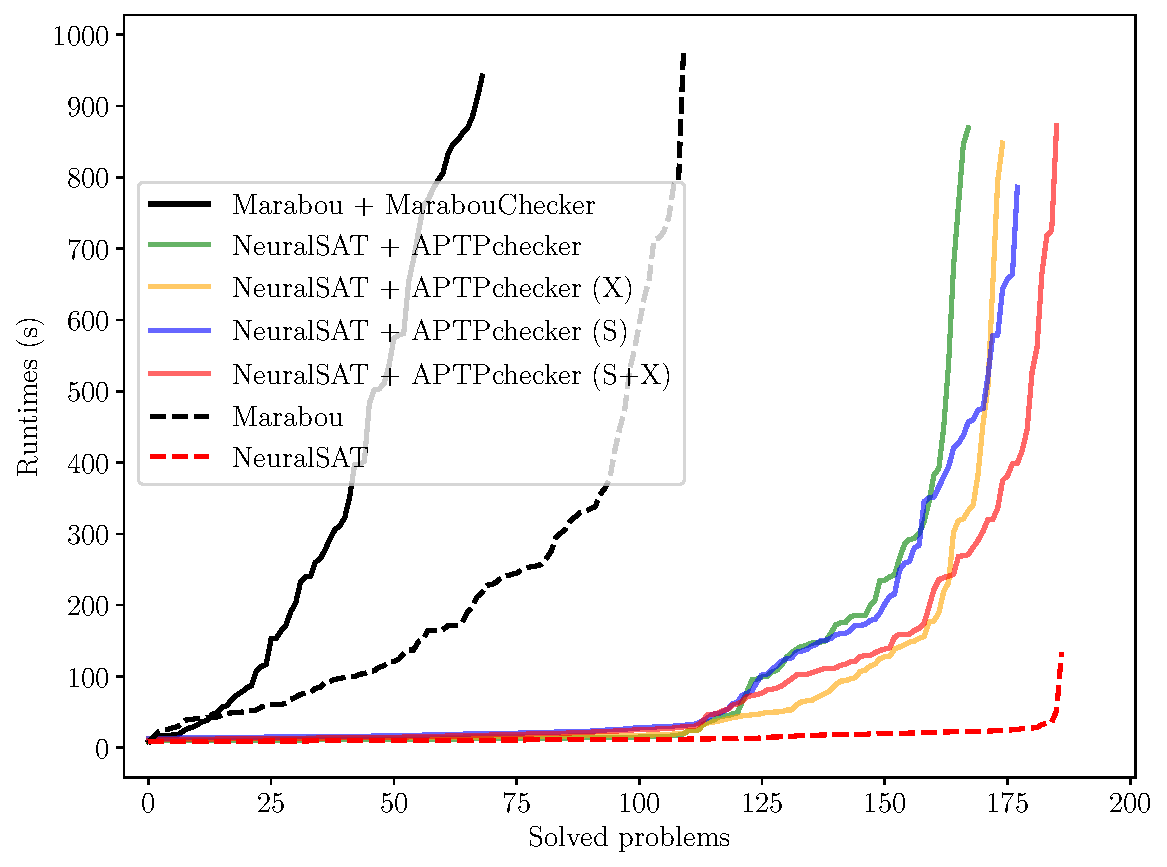
\includegraphics[width=\linewidth]{figure/fnn.pdf}
%     \end{minipage}
%     \begin{minipage}[t]{0.4\textwidth}
%         \centering  
%         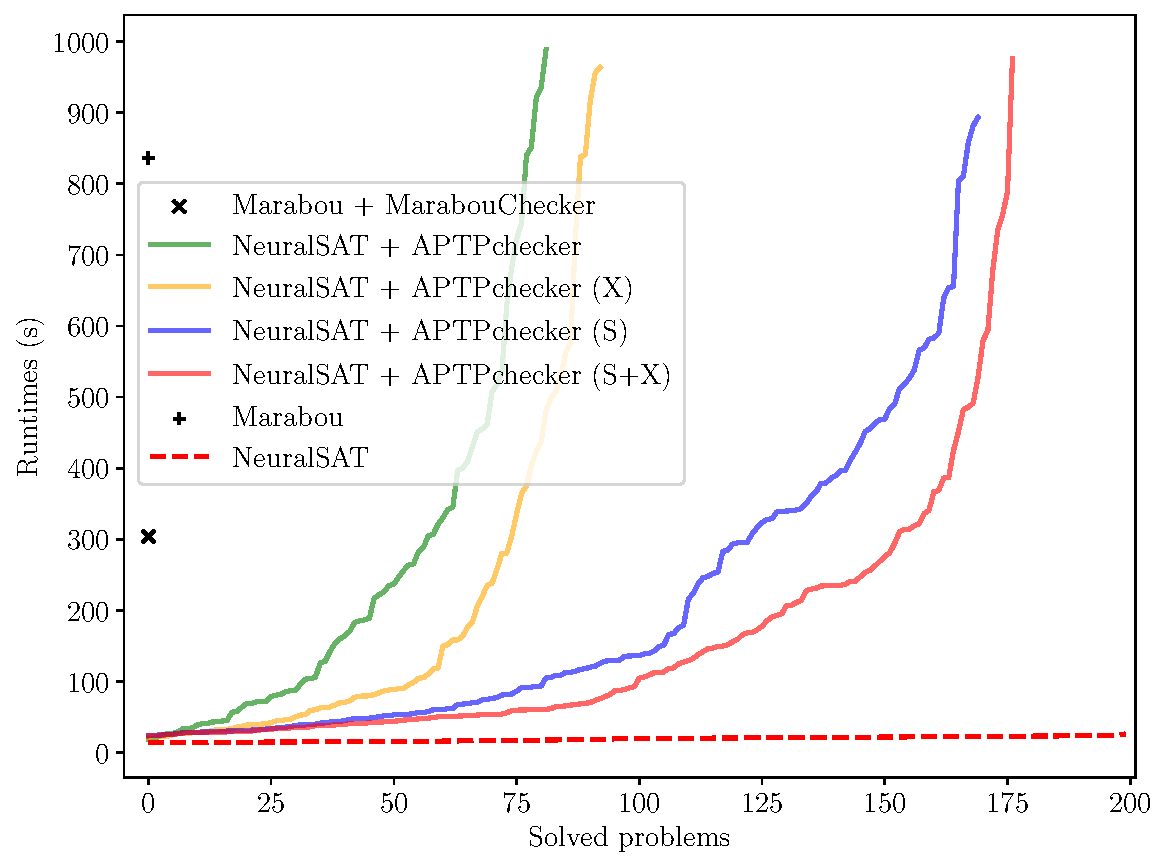
\includegraphics[width=\linewidth]{figure/cnn.pdf}
%     \end{minipage}

%     % \begin{minipage}[t]{0.45\textwidth}
%     %     \centering  
%     %     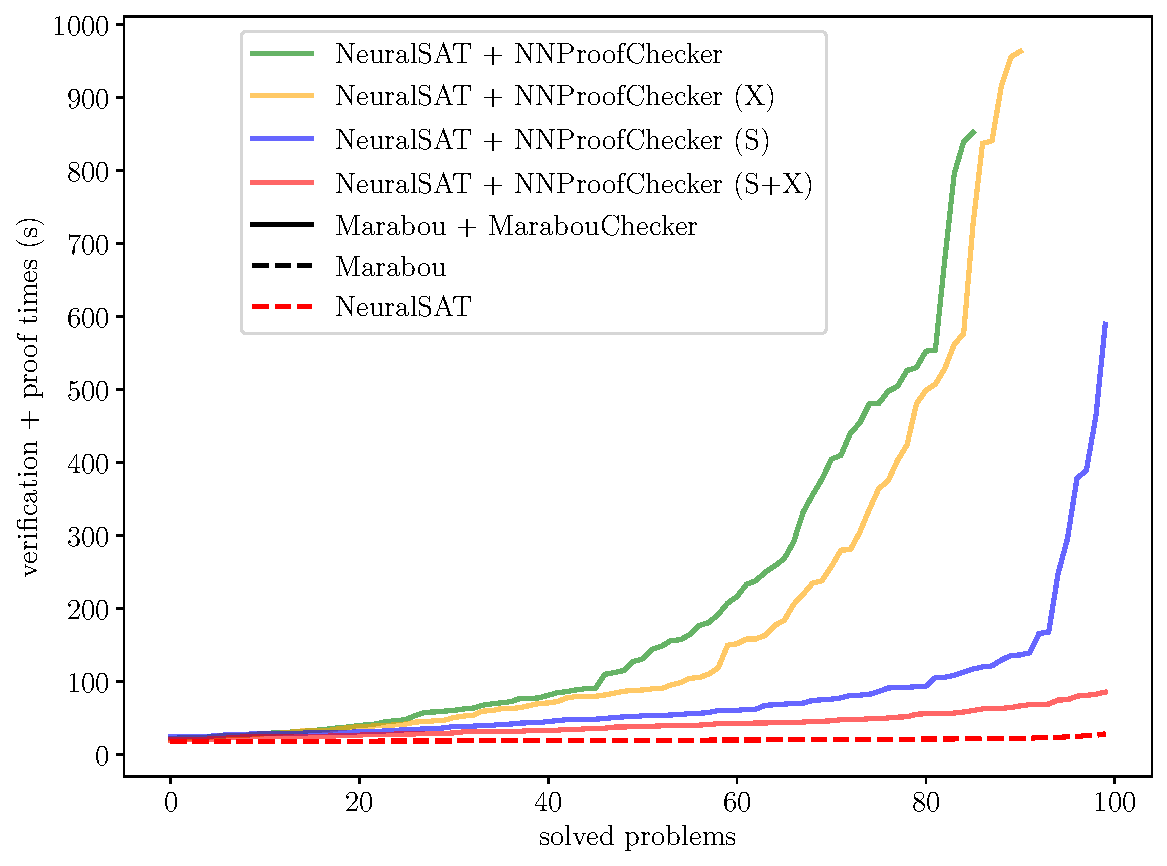
\includegraphics[width=\linewidth]{figure/MNIST_CNN_SMALL.pdf}
%     % \end{minipage}
%     % \hfill
%     % \begin{minipage}[t]{0.45\textwidth}
%     %     \centering  
%     %     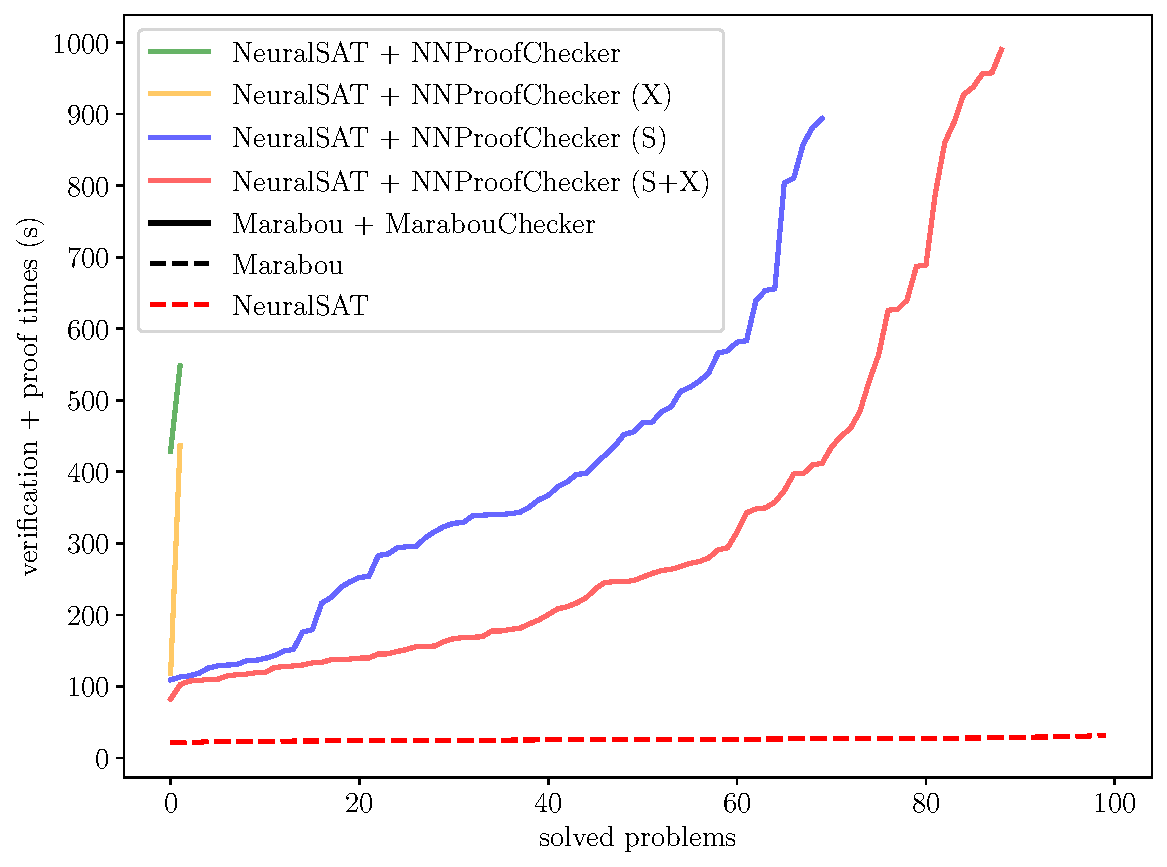
\includegraphics[width=\linewidth]{figure/MNIST_CNN_MEDIUM.pdf}
%     % \end{minipage}
%     \caption{Cactus-plots for verifiers and proof checkers of FNN (top) and CNN (bottom) benchmarks.}
%     \label{fig:cactus-plots}
% \end{figure}
% \paragraph{Treatments}
% RQ1 compares the best performing versions of \marabou{}'s proof checker and \proofcheck{}.
% For RQ2, we consider two of the three optimizations
% implemented in \proofcheck{} : proof tree pruning (X), and 
% proof stabilization (S).  We kept a third optimization that controls the
% degree of parallelization in proof checking fixed at a value of 64 to mitigate
% experimental cost; since the independence of sub-proofs means that
% proof checking is amenable to linear speedup we felt this aspect of experimentation
% was less valuable.
% For RQ3, we use both \neuralsat{} and \crown{} to generate proofs; this
% constitutes a treatment for this research question as it varies the
% verification algorithm.
% For each verifier, we explore a base version of the verifier and an optimization:
% the stabilization optimization for \neuralsat{} and replacing
% the default branch-and-bound decision heuristic with the BaBSR~\cite{bunel2020branch} heuristic
% in \crown{}.

% \paragraph{Metrics}
% In the verification community there are two metrics commonly used to
% assess performance: time to solve the problems and number of problems solved
% from a benchmark.  We report them both here.

% For each \proofcheck{} problem we record:
% the time to verify that the problem is UNSAT, the time to generate a proof,
% the time for \proofcheck{} to finish.
% If the sum of these for a problem is less than a specified timeout,
% 1000 seconds in our evaluation, then we say the problem is ``solved''.
% For verifiers run alone, a problem is solved if the verification completes
% within the timeout.

% For each benchmark, we provide cactus plots which plot the time for a problem on the y-axis, and the number of problems solved on the x-axis; problems are sorted on the x-axis from least to largest.
% As shown in~\autoref{fig:cactus-plots}, these plots allow one to observe both the time difference between baselines and treatments (vertical distance between lines at a point on the x-axis) and the ability of techniques to solve problems (the maximum x-coordinate for a given line).

% We also report the size of proof trees that are generated in \prooflang{}.
% In the absence of optimizations this defines the \textit{number of sub-proofs}
% that need to be checked, but with optimizations the number of sub-proofs may
% be reduced, e.g., when an interior node in the tree can be proven.
% The complexity of  sub-proofs
% may vary significantly, so to provide a more detailed characterization we
% also report \textit{MILP complexity}.  \autoref{eq:mip} defines the general form
% of each MILP problem, but the problems will vary based on how many of the $a$ variables
% defined in \autoref{eq:mip}(d) have a fixed value -- either 0 or 1.   When this
% happens the constraint in \autoref{eq:mip}(e) are simplified.
% Consequently, we measure MILP complexity as the number of neurons that do \textit{not}
% have a fixed value, i.e., the number of unstable neurons.  
% \ignore{This does not account for the contribution of \autoref{eq:mip}a,b which is directly
% related to network size and input/output dimension.   Is there any way to measure that?}
% % \hd{I see. It seems hard since "a"s and constraints do not have the same unit.}

% \paragraph{Experimental Setup}
% All experiments were run on a Linux machine with an AMD Threadripper 64-core 4.2GHZ CPU, 128GB RAM, and an NVIDIA GeForce RTX 4090 GPU with 24 GB VRAM. 
% We used a timeout of 1000 seconds for the combined time of running the verifier,
% generating the proof, and then checking that proof.

% \subsection{RQ1 : Proof Checking Performance}
% \label{sec:rq1}
% \autoref{fig:cactus-plots} presents data on the performance
% of \proofcheck{} relative to both an underlying verifier, \neuralsat{}, and prior work on neural network proof checking, \marabou{}'s proof checker.  
% In cactus plots like this, lines that extend further on the x-axis
% are better -- more problems solved -- and lines that are lower are better -- faster solve times.
% Another way to view these is to pick a point on the x-axis where the plots for two techniques are defined and think of the areas under the two curves as the ``total cost'' to solve that number of problems.
% The dashed lines in the plots show the performance of the verifier and the solid lines show the performance of the verifier, proof generation, and the proof checker.  Several configurations of
% \proofcheck{} are shown, but in this RQ we draw the readers attention
% to the plots for the \proofcheck{}(S+X) configurations; the rest are discussed in detail below.

% The cactus plot for the FNN benchmark (top)
% shows that \marabou{} and its checker are able to solve 69 problems or 35\% of the benchmark, whereas \proofcheck{} can solve 186 or 93\%.  
% For the CNN benchmark (bottom) \marabou{} and its checker can solve a single benchmark, whereas \proofcheck{} can solve 177 problems or 89\%.
% In total, \proofcheck{} solved 363 problems or 91\%, whereas \marabou{}  solved 70 problems or 18\% of all instances.

% \begin{figure*}[t]
% \begin{subfigure}{0.4\linewidth}
%     \centering
%     % 
%     \begin{minipage}[t]{0.75\textwidth}
%         \centering  
%         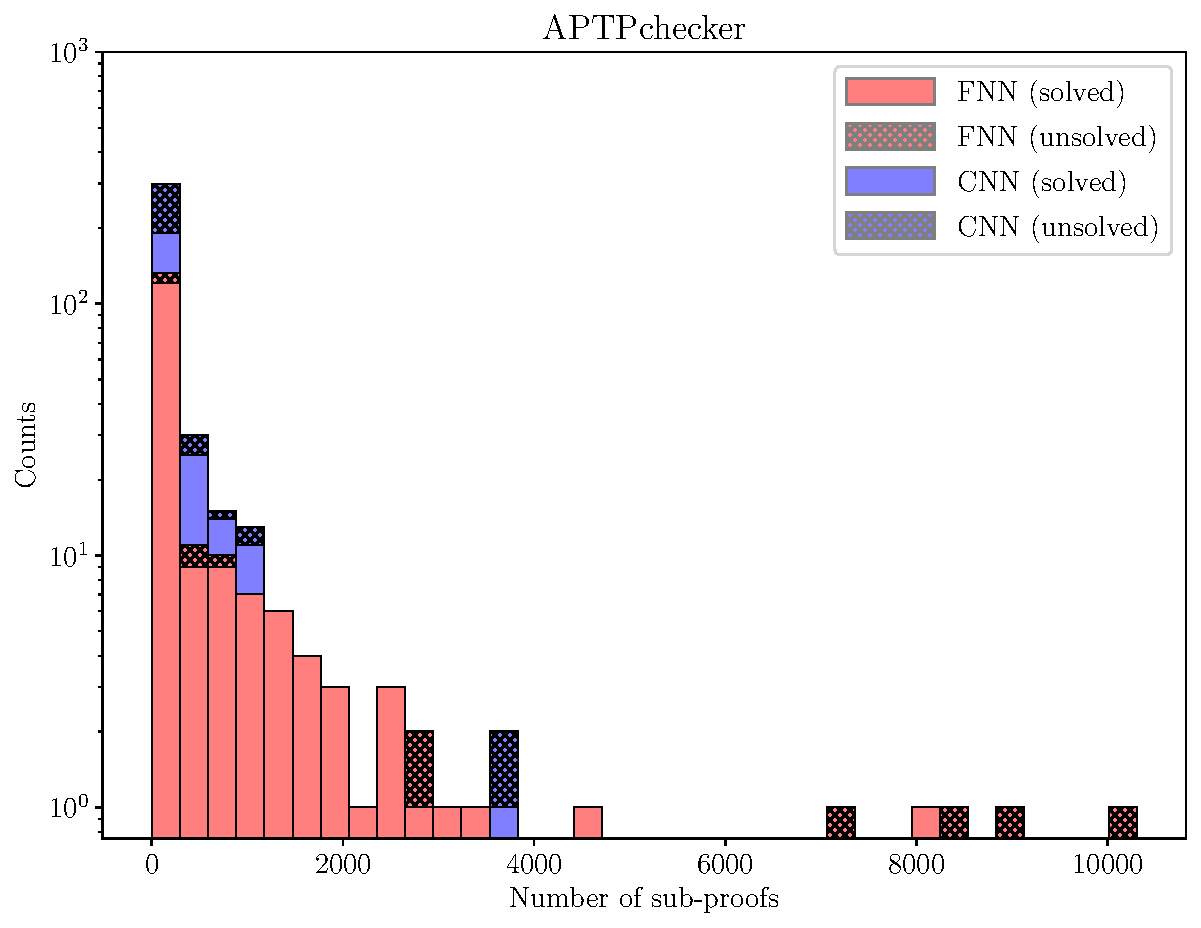
\includegraphics[width=\linewidth]{figure/SUB_PROOFS_NONE.pdf}
%     \end{minipage}
%     %
%     \begin{minipage}[t]{0.235\textwidth}
%         \centering  
%         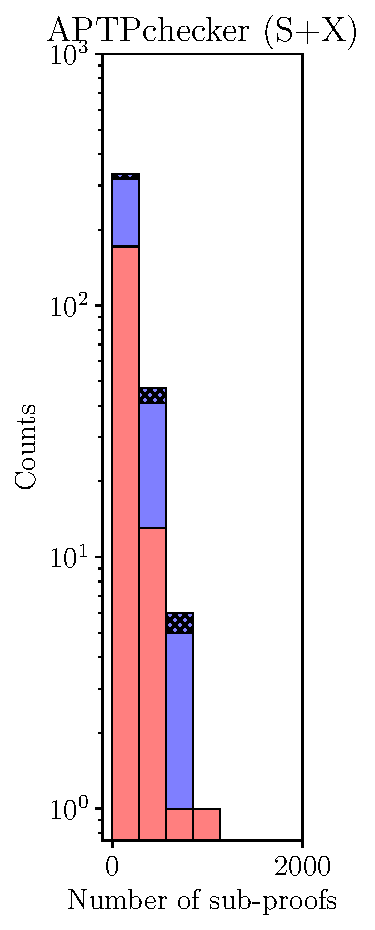
\includegraphics[width=\linewidth]{figure/SUB_PROOFS_SX.pdf}
%     \end{minipage}
%     \caption{Number of sub-proofs per problem with (right) and without (left) \proofcheck{} optimizations.}
%     \label{fig:sub-proofs-plots}
% \end{subfigure}
% \hfill
% \begin{subfigure}{0.59\linewidth}
%     \centering 
%     %
%     \begin{minipage}[t]{0.5\textwidth}
%         \centering  
%         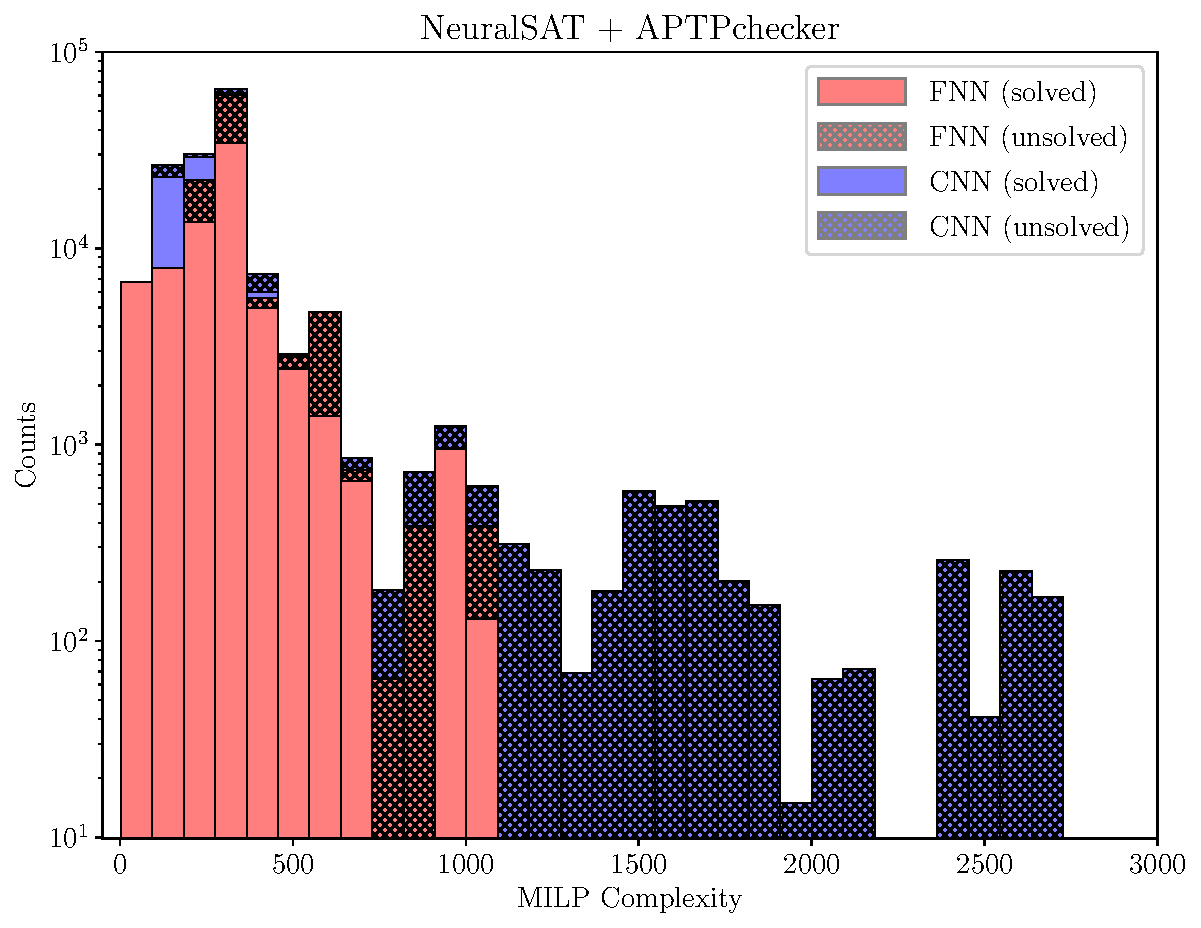
\includegraphics[width=\linewidth]{figure/MILP_COMPLEXITY_NONE.pdf}
%     \end{minipage}%
%     \begin{minipage}[t]{0.5\textwidth}
%         \centering  
%         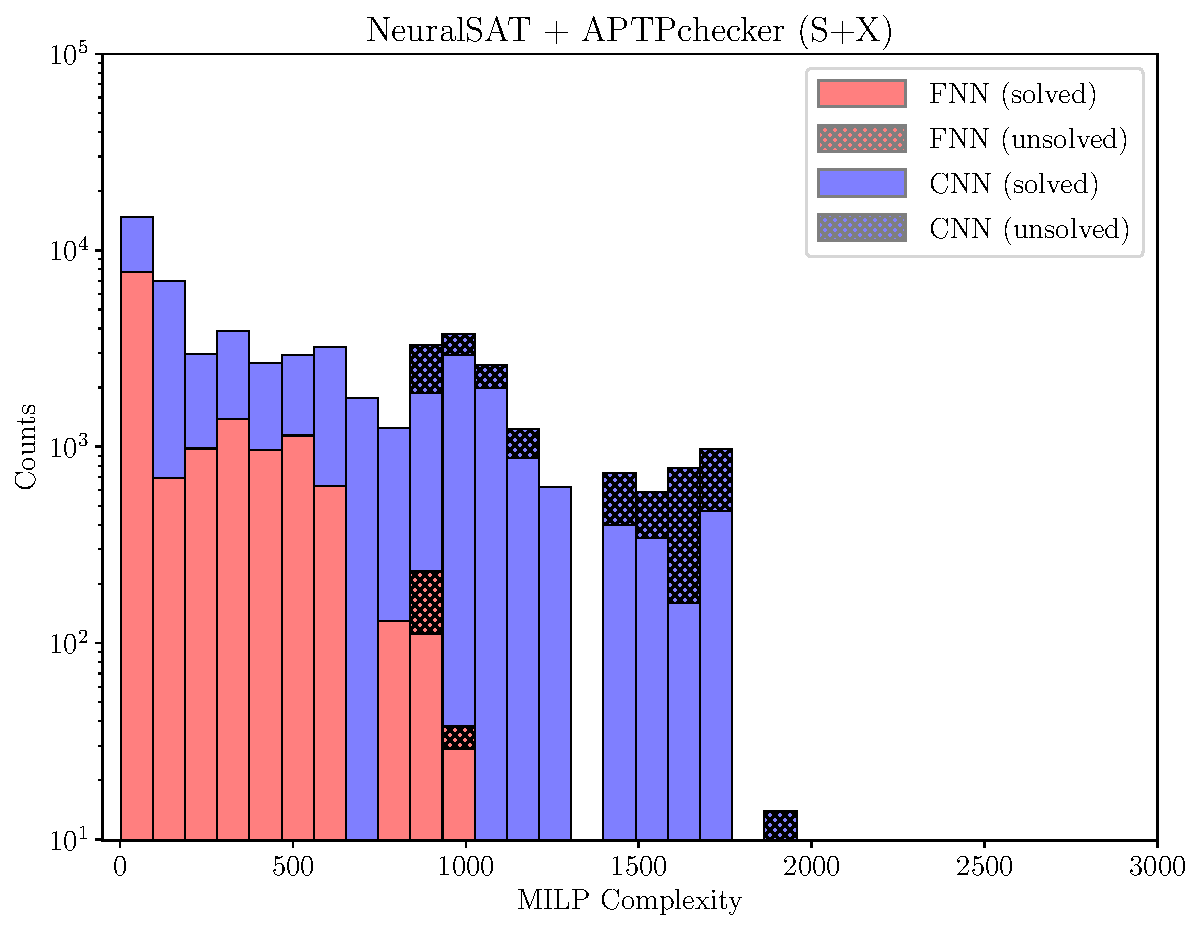
\includegraphics[width=\linewidth]{figure/MILP_COMPLEXITY_SX.pdf}
%     \end{minipage}

%     \caption{Number of constraints of a given complexity per problem with (right) and without (left) \proofcheck{} optimizations.}
%     \label{fig:constrs-proofs-plots}
% \end{subfigure}
% \caption{Data on proof size and complexity.   Y-axes are log-scale due to the range of values.}
% \end{figure*}

% % \matt{Some of the line number references are no longer resolving below.}
% The shape of these cactus plots indicates a high-degree of variability in the cost of proof
% checking relative to verification.
% From~\autoref{fig:algorithm} it is clear that both the number of leaves in the tree
% structure,~\autoref{line:get_leaf}, and the complexity of the model to be checked,~\autoref{line:proof_check_objective1}, are factors that contribute to the cost of proof checking.
% To explore those factors we plot their variation across the benchmarks when running \proofcheck{}.

% \autoref{fig:sub-proofs-plots} (left) plots a histogram of the number of sub-proofs solved per verification 
% problem, i.e., the number of nodes of the proof tree.
% When interpreting these plots, understand that the y-axis log scale means that vertical
% distances have a different meaning as you move upward in the plot.
% While the vast majority of the verification problems have proof trees of fewer then 2000 leaves, but 17 of them have larger trees up to a maximum of more than 10000 leaves.
% Note also that even among the smaller sized proof trees, there are some problems that cannot be solved.
% This is due to complexity of solving the MILP constraints at the leaves of those proof trees.

% \autoref{fig:constrs-proofs-plots} (top) plots a histogram of the number of occurrences of MILP problems of
% a given complexity across the benchmarks.  Here again we see a spread in data, but unlike with the number of sub-proofs the CNN benchmarks seem to have consistently larger constraints and there is a clear bias among the unsolved problems towards larger constraint size.
% To optimize proof checking, we must address both of these sources of complexity.

% \begin{tcolorbox}[left=1pt,right=1pt,top=1pt,bottom=1pt]
% \textbf{RQ1 Findings}: Proof checking performance varies with both the size of the proof tree and the complexity of the MILP problems at the nodes of the tree.  \proofcheck{} can solve 91\% of the problems across the benchmarks and improves on prior work which can solve less than 18\%.
% % \tvn{are these numbers correct?  the 2nd paragraph of RQ1 says prior work can do 24\% and \proofcheck{} can do 92\%}
% \end{tcolorbox}

% \subsection{RQ2 : Proof Checking Optimizations}
% \label{sec:rq2}
% The performance cactus plots~\autoref{fig:cactus-plots} present an ablation
% study of the 
% pruning (X) and stabilization (S) optimizations of \proofcheck{}.
% The trend across both benchmarks is consistent with pruning (yellow) and stabilization (blue)
%  improving the number of problems solved by 5\% and 36\%, respectively, over the unoptimized
% \proofcheck{} (green).
% The combination of optimizations (red) improves the number of solved problems by 46\%, which is more than the sum of their individual improvements demonstrating that the methods create opportunities for one another for further optimization.
% \ignore{
% - neither X nor S: 168 (F) + 88 (C) = 256
% - X: 175 (F) + 93 (C) = 268
% - S: 178 (F) + 170 (C) = 348
% }

% The \autoref{fig:sub-proofs-plots} (right) and \autoref{fig:constrs-proofs-plots} (right) explore the impact of the S and X optimizations on the number of sub-proofs and MILP complexity.  Across the benchmarks optimizations reduce 
% the number of sub-proofs is to less than 1000 and
% MILP complexity to less than 2000.   
% The reduction in sub-proofs directly contributes to the increase
% in performance of \proofcheck{}, but the reduction in
% MILP complexity is more subtle.   
% Integer programming, and thus MILP, is known to be
% NP-Hard in general~\cite{garey1979computers}.
% The stabilization optimization addresses this complexity by
% calculating sets of variables that are forced to take on specific
% values based on other constraints in the MILP problem.  For each
% such variable, the constraints associated with it is effectively
% eliminated.  We can observe this in comparing the left and
% right of \autoref{fig:constrs-proofs-plots} where we see both
% constraints of higher complexity eliminated and the peak of
% the constraint distribution shifted downward from 400 to 100
% constraints.  

% \ignore{
% Sub-problem size
% - without S+X:
%     + mean: 388
%     + std: 1062
% - with S+X
%     + mean: 142
%     + std: 152

% MILP complexity
% - without S+X: 
%     + mean: 329
%     + std: 274
% - with S+X
%     + mean: 493
%     + std 449

% We performed an analysis of the relationship between size of constraints and number of sub-proofs and determined that these factors are not strongly correlated.
% For example, there is a 1 layer CNN model with 27k parameters whose verification
% generates 680 sub-proofs where the complexity of the constraints in that proof are at most 109. 
% On the other end of the spectrum, verification of a 2 layer CNN model with 180k parameters only requires 81 sub-proofs, but those proofs consist of constraints with complexity of at least 1721.
% }

% \begin{tcolorbox}[left=1pt,right=1pt,top=1pt,bottom=1pt]
% \textbf{RQ2 Findings}: The \proofcheck{} optimizations each independently increase the number of proofs that can be checked and in combination they allow
% an additional 46\% of the proofs in the benchmarks to be checked.
% \end{tcolorbox}

% \subsection{RQ3 : Proof Checking and Verifier Optimizations}
% \label{sec:rq3}
% \autoref{fig:algvariation} shows cactus-plots for two configurations of \neuralsat{} and \crown{} generated proofs across the benchmarks.   The performance of the verifiers, dashed lines, differ across configurations and they are able to 
% verify between 337 and 400 problems in the benchmark.
% \ignore{Number of Verified/Proved problems
%     + abcrown(babsr):   337/335 = 99.4%
%     + abcrown:          368/366 = 99.4%
%     + neuralsat(SX):    387/363 = 93.7%
%     + neuralsat(S)(SX): 400/384 = 96%
% }
% For both of the verifiers and configurations,
% \proofcheck{} is able to check between 93.7\% and 99.4\% of the proofs that are generated.
% This demonstrates that the \prooflang{} is able to encode proofs
% generated by differing neural network verification algorithms, and
% that \proofcheck{} can check them.

% % \autoref{tab:sizestats}.
% \begin{figure}[t]
%     \centering
%     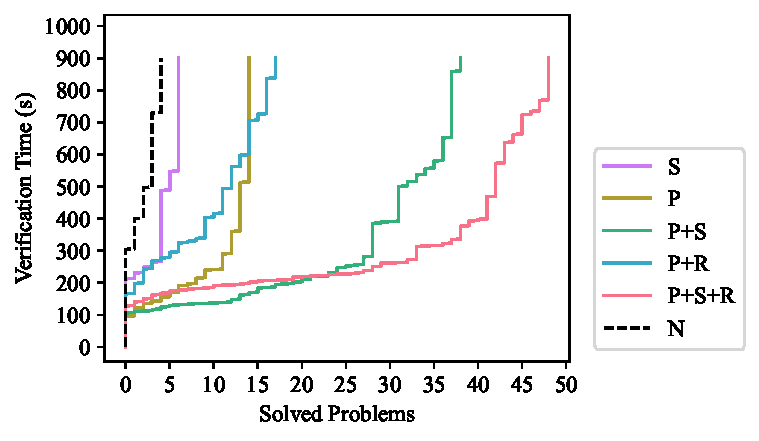
\includegraphics[width=0.8\linewidth]{figure/ablation.pdf}
%     \caption{\proofcheck{} performance with different verification algorithms.}
%     \label{fig:algvariation}
% \end{figure}

% \begin{table}[t]
%     \caption{Proof statistics for best verifier configurations.}
%     \label{tab:sizestats}
%     \centering
%     \begin{tabular}{c|cc|cc}
%         \toprule
%          \multirow{2}{*}{\textbf{Verifier}} & \multicolumn{2}{c}{\textbf{Num. Sub-Proofs}} & \multicolumn{2}{|c}{\textbf{MILP Complexity}}\\
%          & Mean & Median & Mean & Median \\ 
%          \midrule
%          \neuralsat{}(S) & 95 & 36 & 601 & 545 \\ 
%          \midrule
%          \crown{} & 230 & 180 & 414 & 179\\
%          \bottomrule
%     \end{tabular}
% \end{table}

% We performed an analysis of both the number of sub-proofs and MILP complexity for the proofs generated by the two best performing verifier
% configurations.  These values follow a skewed
% distribution, so we report the mean and median values in \autoref{tab:sizestats}.   One can observe variation in the
% structure of the proofs generated by these verifiers.
% \neuralsat{} generates smaller proof trees, but where the
% MILP problems are more complex.
% In contrast, \crown{} generates significantly larger proof trees,
% but with less complex MILP problems.
% This variation suggests potential avenues for future work, especially,
% when proof checking is important.

% For example, \neuralsat{} might include an option to generate larger proof trees, but with smaller MILP problems.  Such proofs would then
% be amenable to higher-degrees of parallel solving and mitigate the 
% performance bottleneck presented by MILP solver implementations.
% One might even consider strategies that use fast verification 
% options during development and then when all properties are proven, shift to slower verification options that are more amenable to proof checking.

% \ignore{
% 1. Longer verification time means proof tree will be larger since verifier has to explore larger space
% 2. If an instance is verified by \crown{}, it will likely be proved by \proofcheck{}. In other words, most of timeout instances are due to \crown{} cannot verify (1st phase).

% - MILP complexity:
%     + neuralsat(S)(SX)  : mean=601.36, std=475.88, median=545.00, min=3, max=1944
%     + neuralsat(SX)     : mean=492.40, std=448.81, median=342.00, min=2, max=1956
%     + abcrown           : mean=414.35, std=447.02, median=179.00, min=0, max=1957
%     + abcrown(babsr)    : mean=409.00, std=448.89, median=166.00, min=0, max=1952

% They share the same MILP base model since their base models are all generated from SX setting.
% neuralsat(S)(SX) has larger MILP complexity in average means that its proof trees are often shallower than others. In other words, neuralsat(S) explores smaller space than others -- which is true.

% - number of sub proofs:
%     + neuralsat(S)(SX): mean=95.11,   std=117.13, median=36.00,  min=0, max=829
%     + neuralsat(SX)   : mean=142.00,  std=151.72, median=106.00, min=1, max=1132
%     + abcrown         : mean=229.96,  std=199.23, median=180.00, min=0, max=1152
%     + abcrown(babsr)  : mean=228.10,  std=170.88, median=188.00, min=0, max=857

% - Number of leaves:
%     + neuralsat(S)(SX): mean=236.59,   std=447.80,   median=37.50,  min=0, max=3627
%     + neuralsat(SX)   : mean=902.25,   std=4957.22,  median=219.00, min=6, max=91318
%     + abcrown         : mean=3007.42,  std=12742.09, median=561.00, min=0, max=138918
%     + abcrown(babsr)  : mean=11714.62, std=41909.72, median=781.50, min=0, max=509765
% }


% \begin{tcolorbox}[left=1pt,right=1pt,top=1pt,bottom=1pt]
% \textbf{RQ3 Findings}: \prooflang{} is robust to variation in different verification algorithms and \proofcheck{} is applicable to any such proof and effective in checking
% the vast majority of those arising from the benchmarks.
% \end{tcolorbox}


\chapter{DNN Verification Benchmarks}\label{chap:benchmarks}
Here we survey the latest benchmarks in DNN verification and how SOTA tools perform on them.  These results are taken from the Verification Neural Network Competitions (VNN-COMP)~\cite{brix2024fifth} and the recent work by Duong et al.~\cite{duong2024harnessing}.




\section{VNN-COMP Benchmarks}

%Artifacts for all benchmarks are available in the repository\footnote{\url{https://github.com/ChristopherBrix/vnncomp2024_benchmarks/tree/main/benchmarks}}.

\tvn{check this table with VNN-COMP'24 reports. The Report seems to have a lot more benchmarks for regular tracks. Also many numbers don't quite match. We should probably use the benchmarks from VNN-COMP'24 report. I also ? on place for you to fill in}

\begin{table}
    \caption{Benchmark instances. U: \texttt{unsat}, S: \texttt{sat}, ?: \texttt{unknown}.}\label{tab:benchmarks}
    \resizebox{\textwidth}{!}{
    \begin{tabular}{c|ccccc|cc}
        \toprule
        \multirow{2}{*}{\textbf{Benchmarks}} &\multicolumn{2}{c}{\textbf{Networks}} &  \multicolumn{3}{c|}{\textbf{Per Network}} &\multicolumn{2}{c}{\textbf{Tasks}} \\
        & Type & Networks & Neurons & Parameters & Input Dim & Properties & Instances (U/S/?) \\
        \midrule
      cGan &  Conv. + Vision Trans. & & & 500K--68M & 5 &  &  \\
      NN4Sys & ReLU + Sigmoid       & & & 33k--37M & 1--308 & & \\
      LinearizeNN & FC. + Conv. + & && 203k & 4 && \\
      &Vision Trans. + Res. + ReLU &&&&&&\\
      \midrule
      Collins RUL CNN & Conv. + ReLU, Dropout  &&& 60k--262k  & 400--800 &&\\
      cifar100 &FC + Conv. + Res., & &&2.5M--3.8M & 3072 & &\\
                                             &ReLU + BatchNorm &&&&&&\\
      tinyimagenet &FC + Conv. + Res., &&& 3.6M & 9408 & &\\
      & ReLU + BatchNorm &&&&&&\\
      Metaroom & Conv. + FC, ReLU &&& 466k--7.4M & 5376 & &\\

      \midrule

      TLL Verify Bench & Two-Level Lattice NN (FC. + ReLU)  &&& 17k--67M & 2 &&\\
      Acas XU & FC. + ReLU &45&300& 13k & 5 &10&139/47/0\\
      %ACAS Xu & FNN & 45 & 300 & 13305 & 5 & 10 & 139/47/0 \\
      Dist Shift & FC. + ReLU + Sigmoid &&& 342k -- 855k & 792 &&\\
      safeNLP & FC. + ReLU &&& 4k & 30 &&\\
      CORA & FC. + ReLU &&& 575k, 1.1M & 784, 3072 &&\\


        % MNISTFC & FNN & 3 &  0.5--1.5K & 269--532K & & 30 & 56/23/11\\

        % %CIFAR2020 & FNN+CNN & 3 &  17--62K & 2.1--2.5M && 203 & 149/43/11 \\
        % \midrule

        % RESNET\_A/B & CNN+ResNet & 2 & 11K & 354K & & 144 & 49/23/72 \\
        % \midrule

        % CIFAR\_GDVB & FNN+CNN & 42 & 9--49K & 0.08--58M && 39 & 60/0/0 \\
        % \midrule
        % \midrule
        % VGGNet16 & CNN + ReLU + MaxPool& ? & ? & 138M & 150K & ? & ? \\
        \bottomrule
        \end{tabular}
    }
\end{table}



\subsection{ACAS Xu}\label{sec:acasxu}
\paragraph{Networks} The ACASXu benchmark consists of 10 properties defined over 45 neural networks used to issue turn advisories to aircraft to avoid collisions. The neural networks have 300 neurons arranged in 6 layers, with ReLU activation functions. There are 5 inputs corresponding to the aircraft states, and 5 network outputs, where the minimum output is used as the turn advisory the system ultimately produces.

\paragraph{Specifications} VNN-COMP uses the original 10 properties~\cite{katz2017reluplex}, where properties 1--4 are checked on all 45 networks as was done in later work by the original authors~\cite{katz2019marabou}. Properties 5--10 are checked on a single network. The total number of benchmarks is therefore 186.\tvn{does not match table}


\subsection{Cifar2020}

\paragraph*{Motivation} This benchmark combines two convolutional CIFAR10 networks from last year's VNN-COMP 2020 with a new, larger network with the goal to evaluate the progress made by the whole field of Neural Network verification.

\paragraph*{Networks} The two ReLU networks \texttt{cifar\_10\_2\_255} and \texttt{cifar\_10\_8\_255} with two convolutional and two fully-connected layers were trained for $\ell_\infty$ perturbations of $\epsilon = \frac{2}{255}$ and $\frac{8}{255}$, respectively, using COLT \cite{balunovic:20}  and the larger \texttt{ConvBig} with four convolutional and three fully-connected networks, was trained using adversarial training \cite{madry:17} and $\epsilon = \frac{2}{255}$.

\paragraph*{Specifications} We draw the first 100 images from the CIFAR10 test set and for every network reject incorrectly classified ones. For the remaining images, the specifications describe a correct classification under an $\ell_\infty$-norm perturbation of at most $\frac{2}{255}$ and $\frac{8}{255}$ for \texttt{cifar\_10\_2\_255} and \texttt{ConvBig} and \texttt{cifar\_10\_8\_255}, respectively and allow a per sample timeout of 5 minutes.


\subsection{VGGNET16}
\paragraph*{Proposed by} Stanley Bak, Stony Brook University

\paragraph*{Motivation} This benchmark tries to scale up the size of networks being analyzed by using the well-studied VGGNET-16 architecture~\cite{simonyan2014very} that runs on ImageNet. Input-output properties are proposed on pixel-level perturbations that can lead to image misclassification. 

\paragraph*{Networks} All properties are run on the same network, which includes 138 million parameters. The network features convolution layers, ReLU activation functions, as well as max pooling layers.

\paragraph*{Specifications} Properties analyzed ranged from single-pixel perturbations to perturbations on all 150528 pixles (L-infinity perturbations). A subset of the images was used to create the specifications, one from each category, which was randomly chosen to attack. Pixels to perturb were also randomly selected according to a random seed.

\paragraph*{Link} \url{https://github.com/stanleybak/vggnet16_benchmark2022/}





% \begin{table}[h]
%     \centering
%     \caption{Overview of all scored benchmarks.}\label{tab:my_label}
%     \resizebox{\textwidth}{!}{
%     \renewcommand{\arraystretch}{1.4}
%     \begin{tabular}{ccccccc}
%     \toprule
%     Category &
%     Benchmark &
%     Application &
%     Network Types &
%     \# Params &
%     Effective Input Dim &
%     Track
%     \\
%     \midrule
%     \multirow{8}{*}{Complex}
%     %& Carvana UNet  & Image Segmentation & Complex UNet              & 275k - 373k & 4.3k \\
%     & cGAN & \makecell{Image Generation \\ \& Image Prediction} & Conv. + Vision Transformer & 500k - 68M & 5 & regular \\
%     & NN4Sys & \makecell{Dataset Indexing \\ \&  Cardinality Prediction}   & ReLU + Sigmoid & 33k - 37M & 1-308 & regular \\
%     %& ml4acopf & Power System & Complex (ReLU + Trigonometric + Sigmoid) & 4k-680k & 22 - 402 & extended \\
%     %& ViT & Vision & Conv. + Residual + Softmax + BatchNorm & 68k - 76k & 3072 & extended \\
%     %& Collins Aerospace & - & FC + Conv. + Residual, LeakyReLU + MaxPool + Square & 1.8M & 1.2M & extended \\
%     %& LSNC & Lyapunov stability of NN controllers & FC + Residual, ReLU + Sin + Cos & 210, 406 & 8 & extended \\
%     %& CCTSDB & - & FC + Conv. + Residual, ReLU +  MaxPool + Clip & 100k & 2 & extended \\
%     %\cmidrule(lr){1-7}
%     %\multirow{7}{*}{\makecell{CNN \\ \& ResNet}}
%     % & Cifar Bias Field      & Image Classification & Conv. + ReLU  & 45k   & 16 \\

%     % & Large ResNets         & Image Classification & ResNet (Conv. + ReLU)  & 55k - 286k   & 3.1k - 12k \\
%     % & Oval21 & Image Classification & Conv. + ReLU  & 3.1k - 6.2k   & 3.1k \\
%     % & SRI ResNet A/B & Image Classification  & ResNet (Conv. + ReLU)  & 11k   & 3.1k \\
%     %& VGGNet16 & Image Classification & Conv. + ReLU + MaxPool    & 138M & 150k & extended \\
%     & Traffic Signs Recognition & Image Classification & Conv. + Sign + MakPool + BatchNorm & 905k - 1.7M & 2.7k - 12k & extended \\

%     % & Yolo & - & FC + Conv. + Residual, ReLU + Sigmoid & 22k - 37M & 1 - 308 & extended \\
%     % %
%     % \cmidrule(lr){1-7} %
%     % \multirow{5.5}{*}{\makecell{FC}}
%     % %& MNIST FC & Image Classification & FC. + ReLU    & 512 - 1.5k & 784 \\
%     % %& Reach Prob Density    & Probability density estimation & FC. + ReLU    & 64 - 192 & 3 - 14 \\
%     % %& RL Benchmarks  & Reinforcement Learning & FC. + ReLU    & 128 - 512  & 4 - 8 \\
%     \bottomrule
%     \end{tabular}
%     }
% \end{table}


\subsection{cGAN}
\paragraph*{Proposed by} Feiyang Cai, Ali Arjomandbigdeli, Stanley Bak (Stony Brook Univ.). Link: \url{https://github.com/feiyang-cai/cgan_benchmark2023}

This benchmark targets robustness verification for generative models—an area often overlooked compared to discriminative networks.
It uses conditional GANs trained to generate images of vehicles at specific distances. The generator takes a 1D distance input and a 4D noise vector; the discriminator outputs a real/fake score and a predicted distance.
Models vary in architecture (CNNs, vision transformers) and image size (32×32, 64×64).
The verification task checks whether the predicted distance from the generated image matches the input condition, under small input perturbations.


\paragraph*{Motivation}
While existing neural network verification benchmarks focus on discriminative models, the exploration of practical and widely used generative networks remains neglected in terms of robustness assessment.
This benchmark introduces a set of image generation networks specifically designed for verifying the robustness of the generative networks.
\paragraph*{Networks}
The generative networks are trained using conditional generative adversarial networks (cGAN), whose objective is to generate camera images that contain a vehicle obstacle located at a specific distance in front of the ego vehicle, where the distance is controlled by the input distance condition.
The network to be verified is the concatenation of a generator and a discriminator.  The generator takes two inputs: 1) a distance condition (1D scalar) and 2) a noise vector controlling the environment (4D vector). The output of the generator is the generated image. The discriminator takes the generated image as input and outputs two values: 1) a real/fake score (1D scalar) and 2) a predicted distance (1D scalar).
Several different models with varying architectures (CNN and vision transformer) and image sizes (32x32, 64x64) are provided for different difficulty levels.
\paragraph*{Specifications}
The verification task is to check whether the generated image aligns with the input distance condition, or in other words, verify whether the input distance condition matches the predicted distance of the generated image.
In each specification, the inputs (condition distance and latent variables) are constrained in small ranges, and the output is the predicted distance with the same center as the condition distance but with slightly larger range.

% %%%%%%%%%%%%%%%%%%%%%%%%%%%%%%

% \pagebreak
% \subsection{NN4Sys}
% \paragraph*{Proposed by} the $\alpha,\!\beta$-CROWN team with collaborations with Cheng Tan, Haoyu He and Shuyi Lin at Northeastern University.
% \paragraph*{Application}
% The benchmark contains networks for database learned index, video streaming learned adaptive bitrate, and learned cardinality
% estimation which map inputs from various dimensions to 1-dimension outputs.

% \begin{itemize}

% \item \textit{Background}: learned index, learned cardinality, and learned
%     adaptive bitrate are all instances in neural networks for computer systems
%         (NN4Sys), which are neural network based methods performing system
%         operations. These classes of methods show great potential but have one
%         drawback---the outputs of an NN4Sys model (a neural network) can be
%         arbitrary, which may lead to unexpected issues in systems.

% \item \textit{What to verify}: our benchmark provides multiple pairs of (1) trained NN4Sys model
% and (2) corresponding specifications. We design these pairs with different parameters such
% that they cover a variety of user needs and have varied difficulties for verifiers. 
% We describe benchmark details in our NN4SysBench report:
%         \url{http://naizhengtan.github.io/doc/papers/nn4sys23lin.pdf}.

% \item \textit{Translating NN4Sys applications to a VNN benchmark}: 
% the original NN4Sys applications have some sophisticated structures that are hard to verify.
% We tailored the neural networks and their specifications to be suitable for VNN-COMP.
% For example, learned index~\cite{kraska18case} contains multiple NNs in a tree structure that together serve one purpose.
% However, this cascading structure is inconvenient/unsupported to verify
% because there is a ``switch" operation---choosing one NN in the second stage
% based on the prediction of the first stage's NN.
% To convert learned indexes to a standard form, we train a monolithic (larger) NN.

% \item \textit{A note on broader impact}: using NNs for systems is a broad topic, but many existing works
% lack strict safety guarantees. We believe that NN Verification can help system developers gain confidence
% to apply NNs to critical systems. We hope our benchmark can be an early step toward this vision.

% \end{itemize}

% \paragraph*{Networks}
% This benchmark has twelve networks with different parameters: two for learned
% indexes, four for learned cardinality estimation and six for learned adaptive bitrate.
% The learned index uses fully-connected feed-forward neural networks. The other
% two---the learned cardinality and the learned adaptive bitrate---has a
% relatively sophisticated internal structure. Please see our NN4SysBench report
% (URL listed above) for details


% \paragraph*{Specifications}
% For learned indexes,
% the specification aims to check if the prediction error is bounded.
% The specification is a collection of pairs of input and output intervals such that
% any input in the input interval should be mapped to the corresponding output interval.
% For learned cardinality estimation and learned adaptive bitrate,
% the specifications check the prediction error bounds (similar to the learned indexes)
% and monotonicity of the networks.
% By monotonicity specifications, we mean that for two inputs, the network should produce a larger
% output for the larger input, which is required by cardinality estimation or adaptive bitrate.


% \paragraph{Link:} \url{https://github.com/Khoury-srg/VNNComp23_NN4Sys}



% %%%%%%%%%%%%%%%%%%%%%%%%%%%%%%%%%%%%%%
% %%%% sec: LinearizeNN %%
% %%%%%%%%%%%%%%%%%%%%%%%%%%%%%%%%%%%%%%
% \subsection{LinearizeNN}
% \paragraph*{Proposed by}  Ali Arjomandbigdeli, Stanley Bak (Stony Brook University).
% \paragraph*{Motivation}
% Assuming having a neural network controller approximation with a piecewise linear model in the form of a set of linear models with added noise to account for local linearization error. The objective of this benchmark is to investigate the neural network output falls within the range we obtain from our linear model output plus some uncertainty.

% The idea of this benchmark came from one of our recent paper~\cite{ArjomandBigdeli2024} in which we approximated the NN controller with a piecewise linear model, and we wanted to check if the neural network output falls within the range we obtained from our linear model output plus some uncertainty.
% \paragraph*{Networks} The neural network controller we used in this benchmark is an image-based controller for an Autonomous Aircraft Taxiing System whose goal is to control an aircraft's taxiing at a steady speed on a taxiway. This network was introduced  in the paper "Verification of Image-based Neural Network Controllers Using Generative Models"~\cite{katz2021veri}. The neural network integrates a concatenation of the cGAN (conditional GAN) and controller, resulting in a unified neural network controller with low-dimensional state inputs. In this problem, the inputs to the neural network consist of two state variables and two latent variables. The aircraft's state is determined by its crosstrack position (p) and heading angle error ($\theta$) with respect to the taxiway center line. Two latent variables with a range of -0.8 to 0.8 are introduced to account for environmental changes.

% Because in this case the output spec depends on both the input and output and considering the VNN-LIB limitation, we added a skip-connection layer to the neural network to have the input values present in the output space. We also added one linear layer after that to create a linear equation for each local model.
% \paragraph*{Specifications} As mentioned earlier, the aim of this benchmark is to examine whether the neural network output stays within the range defined by the linear model's output, including a margin for uncertainty.Given input $x \in X$ and output $Y = f_{NN}(x)$, the query is of the form: $A_{mat}\times X + b + U_{lb} \leq Y \leq A_{mat}\times X + b + U_{ub}$ for each linear model in its abstraction region.
% \paragraph*{Link} \url{https://github.com/aliabigdeli/LinearizeNN_benchmark2024}

% %%%%%%%%%%%%%%%%%%%%%%%%%%%%%%%%%%5
% \pagebreak
% % \subsection{Cifar Bias Field}

% % \paragraph{Proposed by} The VeriNet team.

% % \paragraph*{Motivation} This benchmark considers verification of a Cifar 10 network against bias field perturbations. The bias field perturbations are encoded by creating augmented networks with only 16 input parameters; thus, the problem has a significantly lower input dimensionality than many other image-based benchmarks.

% % \paragraph*{Networks} For each image to be verified, a separate bias field transform network is created~\cite{Henriksen+21} which consists of the FC transform layer followed by the Cifar CNN. The Cifar CNN consists of 8 convolutional layers followed by ReLUs. Each bias field transform network has 363k parameters and 45k nodes.  

% % \paragraph*{Specifications} The specification considers bias field perturbations of the input. The task is reduced to a standard $\ell_\infty$ specification by encoding bias field the bias field transformation into fully connected layers which are prepended to the network under consideration. The bias field perturbations used $\epsilon = 0.06$ (as described in~\cite{Henriksen+21}) and a timeout of 5 minutes. 


% %%%%%%%%%%%%%%%%%%%%%%%%%%%%%%%%%%%%%%
% %%%% sec: ml4acopf %%
% %%%%%%%%%%%%%%%%%%%%%%%%%%%%%%%%%%%%%%
% \subsection{ml4acopf}
% \paragraph*{Proposed by} Haoruo Zhao, Michael Klamkin, Mathieu Tanneau, Wenbo Chen, and Pascal Van Hentenryck (Georgia Institute of Technology), and Hassan Hijazi, Juston Moore, and Haydn Jones (Los Alamos National Laboratory).

% \paragraph*{Motivation}
% Machine learning models are utilized to predict solutions for an optimization model known as AC Optimal Power Flow (ACOPF) in the power system. Since the solutions are continuous, a regression model is employed. The objective is to evaluate the quality of these machine learning model predictions, specifically by determining whether they satisfy the constraints of the optimization model. Given the challenges in meeting some constraints, the goal is to verify whether the worst-case violations of these constraints are within an acceptable tolerance level.

% \paragraph*{Networks}
% The neural network designed comprises two components. The first component predicts the solutions of the optimization model, while the second evaluates the violation of each constraint that needs checking. The first component consists solely of general matrix multiplication (GEMM) and rectified linear unit (ReLU) operators. However, the second component has a more complex structure, as it involves evaluating the violation of AC constraints using nonlinear functions, including sigmoid, quadratic, and trigonometric functions such as sine and cosine. This complex evaluation component is incorporated into the network due to a limitation of the VNNLIB format, which does not support trigonometric functions. Therefore, these constraints violation evaluation are included in the neural network.

% \paragraph*{Specifications}
% In this benchmark, four different properties are checked, each corresponding to a type of constraint violation:
% \begin{enumerate}
%     \item Power balance constraints: the net power at each bus node is equal to the sum of the power flows in the branches connected to that node.
%     \item Thermal limit constraints: power flow on a transmission line is within its maximum and minimum limits.
%     \item Generation bounds: a generator's active and reactive power output is within its maximum and minimum limits.
%     \item Voltage magnitude bounds: a voltage's magnitude output is within its maximum and minimum limits.
% \end{enumerate}

% The input to the model is the active and reactive load. The chosen input point for perturbation is a load profile for which a corresponding feasible solution to the ACOPF problem is known to exist. For the feasibility check, the input load undergoes perturbation. Although this perturbation does not exactly match physical laws, the objective is to ascertain whether a machine learning-predicted solution with the perturbation can produce a solution that does not significantly violate the constraints.

% The scale of the perturbation and the violation threshold are altered by testing whether an adversarial example can be easily found using projected gradient descent with the given perturbation. The benchmark, provided with a fixed random seed, is robust against the simple projected gradient descent that is implemented.

% \paragraph*{Link} \url{https://github.com/AI4OPT/ml4acopf_benchmark}


% %%%%%%%%%%%%%%%%%%%%%%%%%%%%%%%%%%%%%%
% %%%% sec: ViT %%
% %%%%%%%%%%%%%%%%%%%%%%%%%%%%%%%%%%%%%%
% \subsection{ViT}
% \paragraph*{Proposed by} the $\alpha,\!\beta$-CROWN team.
% \paragraph*{Motivation}
% Transformers~\cite{vaswani2017attention} based on the self-attention mechanism have much more complicated architectures and contain more kinds of nonlinerities, compared to simple feedforward networks with relatively simple activation functions. 
% It makes verifying Transformers challenging. We aim to encourage the development of verification techniques for Transformer-based models, and we also aim to benchmark neural network verifiers on relatively complicated neural network architectures and more general nonlinearities. Therefore, we propose a new benchmark with Vision Transformers (ViTs)~\cite{dosovitskiy2020image}. This benchmark is developed based on our work on neural network verification for models with general nonlinearities~\cite{shi2024genbab}.

% \paragraph*{Networks}
% The benchmark contains two ViTs, as shown in \Cref{tab:vits}.
% Considering the difficulty of verifying ViTs, we modify the ViTs and make the models relatively shallow and narrow, with significantly reduced number of layers and attention heads.
% Following \cite{shi2019robustness}, we also replace the layer normalization with batch normalization.
% The models are mainly trained with PGD training~\cite{madry2017towards}, and we also add a weighted IBP~\cite{gowal2018effectiveness,shi2021fast} loss for one of the models as a regularization.

% \begin{table}[ht]
% \centering
% \caption{Networks in the ViT benchmark.}
% \label{tab:vits}
% \begin{tabular}{ccc}
% \toprule 
% Model & \texttt{PGD\_2\_3\_16} & \texttt{IBP\_3\_3\_8} \\
% \midrule
% Layers & 2 & 3\\
% Attention heads & 3 & 3\\
% Patch size & 16 & 8\\
% Weight of IBP loss & 0 & 0.01\\
% Training $\epsilon$ & $\frac{2}{255}$ & $\frac{1}{255}$\\
% Clean accuracy & 59.78\% & 62.21\%\\
% \bottomrule
% \end{tabular}
% \end{table}

% \paragraph*{Specifications} 
% The specifications are generated from the robustness verification problem with $\ell_\infty$ perturbation. 
% We use the CIFAR-10 dataset with perturbation size $\epsilon=\frac{1}{255}$ at test time.
% We have filtered the CIFAR-10 test set to exclude instances where either adversarial examples can be found (by PGD attack~\cite{madry2017towards} with 100 steps and 1000 restarts) or the vanilla CROWN-like method~\cite{zhang2018efficient,shi2019robustness} can already easily verify. 
% We randomly keep 100 instances for each model, with a timeout threshold of 100 seconds. 
% Note that since instances with adversarial examples have mostly been excluded during the filtering process, this version of the benchmark may not be able to reflect soundness issues in verifiers, and we refer readers to \cite{zhou2024testing} for discussions on testing soundness with models including ViT.

% \paragraph*{Link} \url{https://github.com/shizhouxing/ViT_vnncomp2023}


% \subsection{LSNC}

% \paragraph*{Proposed by} the $\alpha,\!\beta$-CROWN team.
% \paragraph*{Motivation}
% We develop a benchmark for the problem of verifying the Lyapunov stability of NN controllers in nonlinear dynamical systems within a region-of-intrest and a region-of-attraction. This is important for providing stability guarantees that are essential for safety-critical applications with NN controllers. It is also a useful application of neural network verification as recently demonstrated in \cite{yang2024lyapunov,shi2024certified}, and we refer readers to those works for more details on the problem.
% \paragraph*{Networks and Specifications}
% Models are adopted from \cite{yang2024lyapunov}. 
% We adopt two models for the 2D quadrotor dynamical system with state feedback and output feedback, respectively. Each model consists of a controller which is a shallow ReLU network, a Lyapunov function which is a quadratic function, and nonlinear operators modelling the dynamics of a 2D quadrotor. The model for output feedback further consists of a shallow LeakyReLU network as the observer. The verification objective of the Lyapunov stability has been encoded in the ONNX graphs and VNNLIB specifications. Specifications for the benchmark are randomly generated and consist of random sub-regions within the original region-of-interest. The size of the random sub-regions is controlled by a factor $\epsilon~(0<\epsilon\leq 1)$ which is applied to each input dimension, and it has been adjusted for a suitable difficulty given the timeout. For the state feedback model, we set $\epsilon=0.5$ and the timeout is 100s; for the output feedback model, we set $\epsilon=0.3$ and timeout is 200s. For each of the two models, we randomly generate 20 instances. 
% \paragraph*{Link} \url{https://github.com/shizhouxing/LSNC_VNNCOMP2024}

% \subsection{Collins-RUL-CNN}
% \paragraph*{Proposed by} Collins Aerospace, Applied Research \& Technology (\href{https://www.collinsaerospace.com/what-we-do/capabilities/technology-and-innovation/applied-research-and-technology}{website}).

% \paragraph*{Motivation} Machine Learning (ML) is a disruptive technology for the aviation industry. This particularly concerns safety-critical aircraft functions, where high-assurance design and verification methods have to be used in order to obtain approval from certification authorities for the new ML-based products. Assessment of correctness and robustness of trained models, such as neural networks, is a crucial step for demonstrating the absence of unintended functionalities~\cite{ForMuLA, kirov2023formal}. The key motivation for providing this benchmark is to strengthen the interaction between the VNN community and the aerospace industry by providing a realistic use case for neural networks in future avionics systems~\cite{kirov2023benchmark}.

% \paragraph*{Application} Remaining Useful Life (RUL) is a widely used metric in Prognostics and Health Management (PHM) that manifests the remaining lifetime of a component (e.g., mechanical bearing, hydraulic pump, aircraft engine). RUL is used for Condition-Based Maintenance (CBM) to support aircraft maintenance and flight preparation. It contributes to such tasks as augmented manual inspection of components and scheduling of maintenance cycles for components, such as repair or replacement, thus moving from preventive maintenance to \emph{predictive} maintenance (do maintenance only when needed, based on component’s current condition and estimated future condition). This could allow to eliminate or extend service operations and inspection periods, optimize component servicing (e.g., lubricant replacement), generate inspection and maintenance schedules, and obtain significant cost savings. Finally, RUL function can also be used in airborne (in-flight) applications to dynamically inform pilots on the health state of aircraft components during flight. Multivariate time series data is often used as RUL function input, for example, measurements from a set of sensors monitoring the component state, taken at several subsequent time steps (within a time window). Additional inputs may include information about the current flight phase, mission, and environment. Such highly multi-dimensional input space motivates the use of Deep Learning (DL) solutions with their capabilities of performing automatic feature extraction from raw data.

% \paragraph*{Networks} The benchmark includes 3 convolutional neural networks (CNNs) of different complexity: different numbers of filters and different sizes of the input space. All networks contain only convolutional and fully connected layers with ReLU activations. All CNNs perform the regression function. They have been trained on the same dataset (time series data for mechanical component degradation during flight).

% \paragraph*{Specifications} We propose 3 properties for the NN-based RUL estimation function. First, two properties (robustness and monotonicity) are local, i.e., defined around a given point. We provide a script with an adjustable random seed that can generate these properties around input points randomly picked from a test dataset. For robustness properties, the input perturbation (delta) is varied between 5\% and 40\%, while the number of perturbed inputs varies between 2 and 16. For monotonicity properties, monotonic shifts between 5\% and 20\% from a given point are considered. Properties of the last type ("if-then") require the output (RUL) to be in an expected value range given certain input ranges. Several if-then properties of different complexity are provided (depending on range widths).

% \paragraph*{Link} \url{https://github.com/loonwerks/vnncomp2022}

% \paragraph*{Paper} Available in~\cite{kirov2023benchmark} or on request.




% %%%%%%%%%%%%%%%%%%%%%%%%%%%%%%%%%%%%%%
% %%%% sec: Traffic Signs Recognition %%
% %%%%%%%%%%%%%%%%%%%%%%%%%%%%%%%%%%%%%%
% \subsection{Traffic Signs Recognition}
% \paragraph*{Proposed by} M\u{a}d\u{a}lina Era\c{s}cu and Andreea Postovan (West University of Timisoara, Romania)
% \paragraph*{Motivation} Traffic signs play a crucial role in ensuring road safety and managing traffic flow in both city and highway driving. The recognition of these signs, a vital component of autonomous driving vision systems, faces challenges such as susceptibility to adversarial examples~\cite{szegedy2013intriguing} and occlusions~\cite{zhang2020lightweight}, stemming from diverse traffic scene conditions.

% \paragraph*{Networks} Binary neural networks (BNNs) show promise in computationally limited and energy-constrained environments within the realm of autonomous driving~\cite{hubara2016binarized}. BNNs, where weights and/or activations are binarized to $\pm 1$, offer reduced model size and simplified convolution operations for image recognition compared to traditional neural networks (NNs).

% We trained and tested various BNN architectures using the German Traffic Sign Recognition Benchmark (GTSRB) dataset~\cite{GTSRB}. This multi-class dataset, containing images of German road signs across 43 classes, poses challenges for both humans and models due to factors like perspective change, shade, color degradation, and lighting conditions. The dataset was also tested using the Belgian Traffic Signs \cite{BelgianTrafficSignDatabase} and Chinese Traffic Signs \cite{ChineseTrafficSignDatabase} datasets. The Belgium Traffic Signs dataset, with 62 classes, had 23 overlapping classes with GTSRB. The Chinese Traffic Signs dataset, with 58 classes, shared 15 classes with GTSRB. Pre-processing steps involved relabeling classes in the Belgium and Chinese datasets to match those in GTSRB and eliminating non-overlapping classes (see \cite{postovan2023architecturing} for details).

% We provide three models with the structure in Figures \ref{fig:Acc-Efficient-Arch-GTSRB-Belgium}, \ref{fig:Acc-Efficient-Arch-Chinese}, and \ref{fig:XNOR(QConv)-arch}. They contain QConv, Batch Normalization (BN), Max Pooling (ML), Fully Connected/Dense (D) layers.  Note that the QConv layer binarizes the corresponding convolutional layer. All models were trained for 30 epochs. The model from Figure \ref{fig:Acc-Efficient-Arch-GTSRB-Belgium} was trained with images having the dimension 64px x 64 px, the one from Figure \ref{fig:Acc-Efficient-Arch-Chinese} with 48px x 48 px and the one from Figure \ref{fig:XNOR(QConv)-arch} with 30px x 30 px. The two models involving Batch Normalization layers introduce real valued parameters besides the binary ones, while the third one contains only binary parameters (see Table \ref{tab:stats}) for statistics.

% \begin{figure}[h]
%   \centering
%     \includegraphics[width=0.7\textwidth]{figure/AccEfficientGTSRBBelgium.png}
%     \caption{Accuracy Efficient Architecture for GTSRB and Belgium dataset}
%     \label{fig:Acc-Efficient-Arch-GTSRB-Belgium}
% \end{figure}

% \begin{figure}[h]
%   \centering
%     \includegraphics[width=0.7\textwidth]{figure/AccEfficientArchChinese.png}
%     \caption{Accuracy Efficient Architecture for Chinese dataset}
%     \label{fig:Acc-Efficient-Arch-Chinese}
% \end{figure}

% \begin{figure}[h]
%   \centering
%     \includegraphics[width=0.3\textwidth]{figure/XNORQConv.png}
%     \caption{XNOR(QConv) architecture}
%     \label{fig:XNOR(QConv)-arch}
% \end{figure}

% % Please add the following required packages to your document preamble:
% % \usepackage{multirow}
% \begin{table}[h]
% \caption{Training and Testing Statistics}
% \label{tab:stats}
% \centering
% \scriptsize
% \begin{tabular}{|c|c|ccc|ccc|}
% \hline
% \multirow{2}{*}{\textbf{Input size}} & \multirow{2}{*}{\textbf{Model name}} & \multicolumn{3}{c|}{\textbf{Accuracy}}                                      & \multicolumn{3}{c|}{\textbf{\#Params}}                                      \\ \cline{3-8} 
%                             &                             & \multicolumn{1}{c|}{\textbf{German}} & \multicolumn{1}{c|}{\textbf{China}} & \textbf{Belgium} & \multicolumn{1}{c|}{\textbf{Binary}}  & \multicolumn{1}{c|}{\textbf{Real}} & \textbf{Total}   \\ \hline
% 64px $\times$ 64px          & Figure \ref{fig:Acc-Efficient-Arch-GTSRB-Belgium}                  & \multicolumn{1}{c|}{96.45}  & \multicolumn{1}{c|}{81.50} & 88.17   & \multicolumn{1}{c|}{1772896} & \multicolumn{1}{c|}{2368} & 1775264 \\ \hline
% 48px $\times$ 48px          & Figure \ref{fig:Acc-Efficient-Arch-Chinese}                  & \multicolumn{1}{c|}{95.28}  & \multicolumn{1}{c|}{83.90} & 87.78   & \multicolumn{1}{c|}{904288}  & \multicolumn{1}{c|}{832}  & 905120  \\ \hline
% 30px $\times$ 30px          & Figure \ref{fig:XNOR(QConv)-arch}                  & \multicolumn{1}{c|}{81.54}  & \multicolumn{1}{c|}{N/A}   & N/A     & \multicolumn{1}{c|}{1005584} & \multicolumn{1}{c|}{0}    & 1005584 \\ \hline
% \end{tabular}
% \end{table}
% \paragraph*{Specifications} To evaluate the \emph{adversarial robustness} of the networks above, we assessed perturbations within the infinity norm around zero, with the radius denoted as $\epsilon = \{1, 3, 5, 10, 15\}$. This involved randomly selecting three distinct images from the GTSRB dataset's test set for each model and generating \textsc{VNNLIB} files for each epsilon in the set. In total, we created 45 \textsc{VNNLIB} files. Due to a 6-hour total timeout constraint for solving all instances, each instance had a maximum timeout of 480 seconds. To review the generated \textsc{VNNLIB} specification files submitted to VNNCOMP 2023, as well as to generate new ones, please refer to \url{https://github.com/apostovan21/vnncomp2023}.

% \paragraph*{Link} \url{https://github.com/apostovan21/vnncomp2023}



% \subsection{CIFAR100}

% \paragraph*{Proposed by} the $\alpha,\!\beta$-CROWN team.
% \paragraph*{Motivation} This benchmark is reused from VNN-COMP 2022 with a reduced complexity (only two out of the four models with medium sizes are retained). 
% See details in Section 4.5 of the report of VNN-COMP 2022~\cite{muller2022vnncomp}.

% \paragraph*{Networks} We provide two ResNet models on CIFAR-100 with different model widths and depths (input dimension $32 \times 32 \times 3$, 100 classes):
% \begin{itemize}
%     \item \texttt{CIFAR100-ResNet-medium}: 8 residual blocks, 17 convolutional layers + 2 linear layers
%     \item \texttt{CIFAR100-ResNet-large}: 8 residual blocks, 19 convolutional layers + 2 linear layers (almost identical to standard ResNet-18 architecture)
% \end{itemize}

% \paragraph*{Specifications} 
% We randomly select 100 images from the CIFAR-100 test set with a verification timeout of 100 seconds for each of the two models. 
% We filtered out the samples which can be verified by vanilla CROWN (which is used during training) to make the benchmark more challenging. The filtering process is done offline on a machine with a GPU due to the large sizes of these models. 
% A small proportion of instances (around 18\%) with adversarial examples have been retained for potentially identifying unsound results. 

% \paragraph*{Link} \url{https://github.com/huanzhang12/vnncomp2024_cifar100_benchmark}


% \subsection{TinyImagenet}

% \paragraph*{Proposed by} the $\alpha,\!\beta$-CROWN team.
% \paragraph*{Motivation} This benchmark is reused from VNN-COMP 2022. See details in Section 4.5 of the report of VNN-COMP 2022~\cite{muller2022vnncomp}.

% \paragraph*{Networks} We provide a ResNet for TinyImageNet (input dimension $64 \times 64 \times 3$, 200 classes):
% \begin{itemize}
%     \item \texttt{TinyImageNet-ResNet-medium}: 8 residual blocks, 17 convolutional layers + 2 linear layers
% \end{itemize}

% \paragraph*{Specifications} We randomly select 200 images from the TinyImageNet test set with a verification timeout of 100 seconds for each of the two models. A filtering procedure has been adopted similar to the CIFAR100 benchmark.

% \paragraph*{Link} \url{https://github.com/huanzhang12/vnncomp2024_tinyimagenet_benchmark}



% \subsection{TLL Verify Bench}
% \paragraph*{Proposed by} James Ferlez (University of California, Irvine)

% \paragraph*{Motivation} This benchmark consists of Two-Level Lattice (TLL) NNs, which have been shown to be amenable to fast verification algorithms (e.g. \cite{FerlezKS22}). Thus, this benchmark was proposed as a means of comparing TLL-specific verification algorithms with general-purpose NN verification algorithms (i.e. algorithms that can verify arbitrary deep, fully-connected ReLU NNs).

% \paragraph*{Networks}  The networks in this benchmark are a subset of the ones used in \cite[Experiment 3]{FerlezKS22}. Each of these TLL NNs has $n=2$ inputs and $m=1$ output. The architecture of a TLL NN is further specified by two parameters: $N$, the number of local linear functions, and $M$, the number of selector sets. This benchmark contains TLLs of sizes $N = M = 8, 16, 24, 32, 40, 48, 56, 64$, with $30$ randomly generated examples of each (the generation procedure is described in \cite[Section 6.1.1]{FerlezKS22}). At runtime, the specified verification timeout determines how many of these networks are included in the benchmark so as to achieve an overall 6-hour run time; this selection process is deterministic. Finally, a TLL NN has a natural representation using multiple computation paths \cite[Figure 1]{FerlezKS22}, but many tools are only compatible with fully-connected networks. Hence, the ONNX models in this benchmark implement TLL NNs by ``stacking'' these computation paths to make a fully connected NN (leading to sparse weight matrices: i.e. with many zero weights and biases). The \texttt{TLLnet} class (\url{https://github.com/jferlez/TLLnet}) contains the code necessary to generate these implementations via the \texttt{exportONNX} method.

% %\vfill
% %\pagebreak
% \paragraph*{Specifications}  All specifications have as input constraints the hypercube $[-2,2]^2$. Since all networks have only a single output, the output properties consist of a randomly generated real number and a randomly generated inequality direction. Random output samples from the network are used to roughly ensure that the real number property has an equal likelihood of being within the output range of the NN and being outside of it (either above or below all NN outputs on the input constraint set). The inequality direction is generated independently and with each direction having an equal probability. This scheme biases the benchmark towards verification problems for which counterexamples exist. 

% \paragraph*{Link} \url{https://github.com/jferlez/TLLVerifyBench}
% \paragraph*{Commit}
% 199d2c26d0ec456e62906366b694a875a21ff7ef





% %%%%%%%%%%%%%%%%%%%%%%%%%%%%%%
% \subsection{safeNLP}

% \begin{figure}[htbp]
%     \centering
%     \includegraphics[width=0.9\columnwidth]{./figure/NLP-Flow.png}
%     \caption{\small\emph{Generic approach to generating the NLP verification pipelines~\cite{casadio2023antonio,casadio2024nlp} deployed to obtain the safeNLP benchmark.}}
%    \label{fig:antonio}
% \end{figure}

% \paragraph*{Proposed by} Marco Casadio, Ekaterina Komendantskaya, Luca Arnaboldi, Tanvi Dinkar.

% \paragraph*{Motivation}
% While considerable research has been dedicated to the verification of DNN-based systems in domains such as computer vision, there has been a notable lack of focus on the verification of natural language processing (NLP) systems. This is particularly critical given the rise of conversational agents across various domains, where inaccurate or misleading responses can cause real-world harm. For example, recent EU legislation~\cite{EUlaw} requires chatbots to disclose their non-human nature when queried, and developers of the chatbots should provide firm, and if possible, formal, guarantees that such disclosure will be given in an accurate manner. Medical assistants give another example where formal guarantees about the conversational agent responses are needed in order to safeguard against chatbots  generating harmful medical advice~\cite{bickmore2018patient}. While some initial work has been done in this area of NLP verification~\cite{jia2019certified,huang2019achieving,welbl2020towards,zhang2021certified,wang2023robustness,ko2019popqorn,du2021cert,shi2020robustness,bonaert2021fast}, no agreement on commonly  accepted benchmarks has been reached in this domain. To address this gap, we introduce safeNLP, the first such benchmark. 

% \paragraph*{Application}
% In~\cite{casadio2024nlp}, we have undertaken a large-scale study of the existing literature on  NLP verification, and distilled common patterns among the existing approaches. Usually, given a dataset consisting of sentences divided into classes, Large Language Models (LLMs) are used to embed these sentences into real-vector spaces, after which smaller neural networks are trained to classify the embedded vectors (relative to the originally given classes). For verification, one can generate meaning-preserving sentence perturbations, again embed them into vector spaces, and verify that subspaces that contain the (embeddings of) the perturbed sentences are classified correctly. Also, in line with classical verification pipelines~\cite{CasadioKDKKAR22}, one can use these input subspaces to train the neural network to be robust on them.  The problem was that each of the existing approaches~\cite{jia2019certified,huang2019achieving,welbl2020towards,zhang2021certified,wang2023robustness,ko2019popqorn,du2021cert,shi2020robustness,bonaert2021fast} used parts of this pipeline in different ways, which made it difficult to compare or audit the results. In~\cite{casadio2023antonio,casadio2024nlp}, we made a generic implementation of this pipeline, 
% %(released as a Python package ANTONIO), 
% where each of the components of the pipeline is implemented in a modular and transparent way. For example, we can choose  and vary embedding functions, training modes, algorithms for sentence perturbations and algorithms for robust training, independently and modularly; as shown in Figure~\ref{fig:antonio}. This implementation was used to generate the presented VNNCOMP benchmark.

% \begin{itemize}
%     \item \emph{Datasets:} Although there was no clear consensus in~\cite{jia2019certified,huang2019achieving,welbl2020towards,zhang2021certified,wang2023robustness,ko2019popqorn,du2021cert,shi2020robustness,bonaert2021fast}, the most frequently used dataset in prior works was the IMDB dataset containing film reviews. Its disadvantage is unclear relation to safety critical domains that usually motivate verification efforts. On the other hand, none of the previously used datasets concerned safety-critical applications of NLP. We decided to address this problem, and therefore applied our generic NLP verification pipeline on two safety-critical datasets:  R-U-A-Robot~\cite{gros2021ruarobot}, which focuses on the chatbot disclosure problem, and Medical~\cite{abercrombie2022risk}, which addresses the issue of harmful advice provided by medical chatbots. Both datasets are pre-processed into two classes, positive and negative, to simplify the verification task. For further details on the pre-processing steps and datasets, see~\cite{casadio2024nlp} and the \href{https://github.com/ANTONIONLP/safeNLP}{benchmark GitHub repository}.
%     \item \emph{Input Space:} In both datasets, sentences are transformed into fixed-size vector representations, i.e. embeddings, which serve as the inputs to the neural networks. For this VNNCOMP benchmark, we used Sentence-BERT~\cite{reimers-gurevych-2019-sentence}. 
%     %This part is handled by ANTONIO, which employs .
%     \item \emph{What to Verify:} For each dataset, we generated meaning-preseving sentence perturbations at character and word level as in Moradi et al.~\cite{moradi2021evaluating} and at sentence level with Vicuna~\cite{vicuna2023}. For each positive sentence in the dataset, the smallest hypercube containing the embeddings of all of its obtained perturbations formed one input subspace for verification. Such subspaces were obtained for all positive sentences from the given data set, and were subject to VNCCOMP verification challenge. 
%     %ANTONIO’s modular approach allows us to independently chose both the perturbation algorithms and the subspaces form.
%     %The goal is to verify that every point within these subspaces is classified as positive by the network.
%     \item \emph{A note on broader impact:} Verified models can serve as filters for larger NLP systems: e.g. to screen inputs to ensure they meet safety criteria before being passed on to more complex models.
% \end{itemize}

% \paragraph*{Networks} The safeNLP benchmark includes two neural networks, each corresponding to a different dataset (R-U-A-Robot and Medical). Both networks share the same architecture, consisting of two fully-connected layers. The hidden layer has 128 units with a ReLU activation function, while the output layer has 2 units representing the two classification classes (positive/negative). To enhance the robustness of the networks to the specified safety requirements, they are trained using a custom PGD (Projected Gradient Descent)~\cite{madry2018towards} adversarial training technique. In particular, the PGD attack explores the above-mentioned subspaces of the input space (cf. also Figure~\ref{fig:antonio}). 
% %ANTONIO plays a crucial role in this process, allowing us to
% %flexibly select the training mode and robustness algorithm. Specifically, we 
% %customise the PGD algorithm to work effectively with the subspaces used in our specifications.

% \paragraph*{Specifications} The benchmark uses hyper-rectangles in the 30-dimensional embedding space as the subspaces of choice, offering a computationally efficient way to define more precise and adaptable regions compared to the traditional $\epsilon$-cubes. 
% %These hyper-rectangles are defined by a series of lower and upper bounds. 
% The specifications require verifying that, for a given network and hyper-rectangle, every point within the hyper-rectangle is classified as the positive class by the network. To meet time constraints, we randomly select 1,080 such specifications, each linked to one of the two networks and a corresponding hyper-rectangle, with a timeout of 20 seconds per specification.

% \paragraph*{Link} \url{https://github.com/ANTONIONLP/safeNLP}


% %%%%%%%%%%%%%%%%%%%%%%%%%%%%%%%%%%%%%%
% %%%% sec: dist_shift %%
% %%%%%%%%%%%%%%%%%%%%%%%%%%%%%%%%%%%%%%
% \subsection{Real-world distribution shifts}
% \paragraph*{Proposed by} the Marabou team.
% \paragraph*{Motivation}
% While robustness against handcrafted perturbations (e.g., norm-bounded) for perception networks are more commonly investigated, robustness against real-world distribution shifts~\cite{wu2022toward} are less studied but of practical interests. This benchmark set contains queries for verifying the latter type of robustness.  
% \paragraph*{Networks} The network is a concatenation of a generative model and a MNIST classifier. The generative model is trained to take in an unperturbed image and an embedding of a particular type of distribution shifts in latent space, and produce a perturbed image. The distribution shift captured in this case is the "shear" perturbation. 
% \paragraph*{Specifications} The verification task is to certify that a classifier correctly classifies all images in a perturbation set, which is a set of images generated by the generative model given a fixed image and a ball centering the mean perturbations on this image (in the latent space). This mean perturbation is computed by a prior network.
% \paragraph*{Link} \url{https://github.com/wu-haoze/dist-shift-vnn-comp}


% %%%%%%%%%%%%%%%%%%%%%%%%%%%%%%%%%%%%%%
% %%%% sec: cora %%
% %%%%%%%%%%%%%%%%%%%%%%%%%%%%%%%%%%%%%%
% \subsection{CORA Benchmark}
% \paragraph*{Proposed by} the CORA team.
% \paragraph*{Motivation}
% The verification of neural networks can be quite slow, i.e., the verification of a single instance can take multiple days -- which is often hard to justify, particularly in safety-critical scenarios. To encourage the fast verification of neural networks, our benchmark focuses on the verification time by setting a small timeout and testing three different (adversarial) training techniques that aim to ease the verifiability.


% \paragraph*{Networks} The benchmark consists of one ReLU-neural network architecture (7x250 + ReLU), which was trained on three datasets, (MNIST, SVHN, and CIFAR10), using three different (adversarial) training methods, i.e., standard (point), interval-bound propagation, and set-based. Both interval-bound propagation and set-based training are training methods that improve the robustness of the trained neural network and aim to ease later verification. The neural networks are taken from the first evaluation run of~\cite{koller_et_al_2024}; please refer to~\cite{koller_et_al_2024} for the training details.
% \paragraph*{Specifications} All networks are trained on classification tasks. The goal is to verify that no image within a given input set is incorrectly classified.
% \paragraph*{Link} \url{https://github.com/kollerlukas/cora-vnncomp2024-benchmark}

% \section{Results}


% \paragraph{Results} \autoref{tab:score} shows the results. We report the Rank (\textbf{\#}) and  \textbf{\%} is the percentage of solved problems over all problem instances of the corresponding benchmark.   The last two columns break down the number of problems each verifier was able to verify and falsify. For example, for ACAS Xu, all tools other than \crowndefault{} were able to verify all 186 problems (139 + 47), and \crowndefault{} was only able to solve 113 problems (78 + 35), which is 60.8\% of the total problems. 

% \newcommand{\nsTwentyFour}{\texttt{NeuralSAT}$_\text{VNN-COMP'24}$}
% \newcommand{\ns}{\texttt{NeuralSAT}}

% \begin{table}
%   \small
%   \centering
%   \caption{Results over VNN-COMP'24 Benchmarks}\label{tab:score}
%        \renewcommand{\arraystretch}{0.6}
%   \begin{tabular}{c|ccr|rr}
%     \toprule
%     \textbf{Benchmark} & \textbf{\#} & \textbf{Tool} & \textbf{\%} & \textbf{Verify} & \textbf{Falsify}  \\

% \midrule
% \multirow{4}{*}{\rotatebox[origin=c]{0}{ACAS Xu}}
% & 1 & \crown{} & 100.0\% & \textbf{139} & \textbf{47} \\
% & 1 & \ns{} & 100.0\% & \textbf{139} & \textbf{47} \\
% & 1 & \nsTwentyFour{} & 100.0\% & \textbf{139} & \textbf{47} \\
% & 4 & \crowndefault{} & 60.8\% & 78 & 35 \\
% \midrule
% \multirow{4}{*}{\rotatebox[origin=c]{0}{Cgan}} 
% & 1 & \crown{} & 100.0\% & \textbf{8} & \textbf{13} \\
% & 1 & \ns{} & 100.0\% & \textbf{8} & \textbf{13} \\
% & 1 & \nsTwentyFour{} & 100.0\% & \textbf{8} & \textbf{13} \\
% & 4 & \crowndefault{} & 33.3\% & 0 & 7 \\
% \midrule
% \multirow{4}{*}{\rotatebox[origin=c]{0}{Cifar100}} 
% & 1 & \crown{} & 77.5\% & \textbf{123} & \textbf{32} \\
% & 2 & \ns{} & 76.5\% & 122 & 31 \\
% & 3 & \crowndefault{} & 71.0\% & 110 & \textbf{32} \\
% & 4 & \nsTwentyFour{} & 64.5\% & 98 & 31 \\
% \midrule
% \multirow{4}{*}{\rotatebox[origin=c]{0}{Collins Rul CNN}} 
% & 1 & \crown{} & 100.0\% & \textbf{30} & \textbf{32} \\
% & 1 & \crowndefault{} & 100.0\% & \textbf{30} & \textbf{32} \\
% & 1 & \ns{} & 100.0\% & \textbf{30} & \textbf{32} \\
% & 1 & \nsTwentyFour{} & 100.0\% & \textbf{30} & \textbf{32} \\
% \midrule
% \multirow{4}{*}{\rotatebox[origin=c]{0}{Cora}} 
% & 1 & \crown{} & 43.9\% & \textbf{24} & \textbf{134} \\
% & 1 & \crowndefault{} & 43.9\% & \textbf{24} & \textbf{134} \\
% & 1 & \ns{} & 43.9\% & \textbf{24} & \textbf{134} \\
% & 1 & \nsTwentyFour{} & 43.9\% & \textbf{24} & \textbf{134} \\
% \midrule
% \multirow{4}{*}{\rotatebox[origin=c]{0}{Dist Shift}} 
% & 1 & \crown{} & 100.0\% & \textbf{64} & \textbf{8} \\
% & 1 & \ns{} & 100.0\% & \textbf{64} & \textbf{8} \\
% & 3 & \nsTwentyFour{} & 98.6\% & 63 & \textbf{8} \\
% & 4 & \crowndefault{} & 94.4\% & 60 & \textbf{8} \\
% \midrule
% \multirow{4}{*}{\rotatebox[origin=c]{0}{Linearize NN}} 
% & 1 & \crown{} & 100.0\% & \textbf{59} & \textbf{1} \\
% & 1 & \ns{} & 100.0\% & \textbf{59} & \textbf{1} \\
% & 1 & \nsTwentyFour{} & 100.0\% & \textbf{59} & \textbf{1} \\
% & 4 & \crowndefault{} & 68.3\% & 40 & \textbf{1} \\
% \midrule
% \multirow{4}{*}{\rotatebox[origin=c]{0}{Meta Room}} 
% & 1 & \crown{} & 98.0\% & \textbf{91} & \textbf{7} \\
% & 1 & \ns{} & 98.0\% & \textbf{91} & \textbf{7} \\
% & 1 & \nsTwentyFour{} & 98.0\% & \textbf{91} & \textbf{7} \\
% & 4 & \crowndefault{} & 0.0\% & 0 & 0 \\
% \midrule
% \multirow{4}{*}{\rotatebox[origin=c]{0}{Nn4sys}} 
% & 1 & \crown{} & 100.0\% & \textbf{194} & 0 \\
% & 1 & \ns{} & 100.0\% & \textbf{194} & 0 \\
% & 1 & \nsTwentyFour{} & 100.0\% & \textbf{194} & 0 \\
% & 4 & \crowndefault{} & 4.1\% & 8 & 0 \\
% \midrule
% \multirow{4}{*}{\rotatebox[origin=c]{0}{Safe NLP}} 
% & 1 & \crown{} & 98.1\% & \textbf{411} & \textbf{648} \\
% & 1 & \ns{} & 98.1\% & \textbf{411} & \textbf{648} \\
% & 3 & \crowndefault{} & 96.9\% & 401 & 646 \\
% & 4 & \nsTwentyFour{} & 94.3\% & 378 & 640 \\
% \midrule
% \multirow{4}{*}{\rotatebox[origin=c]{0}{Tiny ImageNet}} 
% & 1 & \crown{} & 91.5\% & \textbf{140} & \textbf{43} \\
% & 2 & \ns{} & 91.0\% & 139 & \textbf{43} \\
% & 3 & \crowndefault{} & 89.5\% & 136 & \textbf{43} \\
% & 4 & \nsTwentyFour{} & 72.5\% & 102 & \textbf{43} \\
% \midrule
% \multirow{4}{*}{\rotatebox[origin=c]{0}{TLL Verify Bench}} 
% & 1 & \crown{} & 100.0\% & \textbf{15} & \textbf{17} \\
% & 1 & \ns{} & 100.0\% & \textbf{15} & \textbf{17} \\
% & 1 & \nsTwentyFour{} & 100.0\% & \textbf{15} & \textbf{17} \\
% & 4 & \crowndefault{} & 65.6\% & 5 & 16 \\
% \midrule
% \multirow{4}{*}{\rotatebox[origin=c]{0}{\textbf{Overall}}} 
% & 1 & \crown{} & 88.8\% & \textbf{1298} & \textbf{982} \\
% & 2 & \ns{} & 88.7\% & 1296 & 981 \\
% & 3 & \nsTwentyFour{} & 84.7\% & 1201 & 973 \\
% & 4 & \crowndefault{} & 71.9\% & 892 & 954 \\
% \bottomrule
%   \end{tabular}
% \end{table}


\chapter{VNN-COMPs}\label{chap:vnncomps}

\chapter{Benchmarks Generation}\label{chap:benchmarks-generation}




\chapter{Conclusion}

\appendix

\chapter{Comparing neural networks with software}\label{app:nn-vs-software}

\begin{table}
    \caption{Similarities}\label{tab:nn-software-similarities}
    \scriptsize
    \centering
\begin{tabular}{l|l}
    \toprule
    Aspect & Description\\
    \midrule
    Representation &	Represented using if-then-else statements\\
    Input-Output Mapping &	Take Inputs and produce outputs\\
    Determinism	& Can produce deterministic outputs\\
    Execution Path	& Paths from input to output\\
    Specifications & Can have specifications involving preconditions over inputs and postconditions over outputs\\
    Logical Constraints	& Can be represented as logical constraints\\
    Bugs and Errors & Can have bugs that violate specifications\\
    \bottomrule
\end{tabular}    
\end{table}

\begin{table}
    \caption{Differences}\label{tab:nn-software-differences}
    \scriptsize
    \centering
\begin{tabular}{l|l|l}
    \toprule
    Aspect	& Traditional Software	& Neural Networks \\
    \midrule
    % Control Flow	Complex flow with loops, recursion, and branching.	Feedforward execution; no explicit loops or recursion during inference.
    % State Representation	Uses variables, objects, and explicit state transitions.	Encodes state in weights and neuron activations.
    % Granularity	Operates at a higher abstraction level with fewer conditional branches.	Operates on thousands or millions of neurons, creating many implicit conditional branches.
    % Object-Oriented Features	Incorporates OOP principles like encapsulation, inheritance, and polymorphism.	Lacks explicit OOP features but can be modular (e.g., layers, sub-networks).
    % Execution Path	Determined by explicit logic and relatively few branches.	Implicit execution paths defined by piecewise-linear regions from activations.
    % Termination	Explicitly handles termination in loops and recursion.	Fixed-length inference process with no explicit termination conditions.
    % Semantics	Implements precise, deterministic logic for well-defined tasks.	Approximates functions based on training, often non-deterministic during learning.
    % Verification	Formal verification methods are established for correctness.	Verification is challenging due to non-linearity and high dimensionality.
    % Debugging	Tools like debuggers allow step-by-step inspection of logic.	Focuses on diagnosing data issues, architecture problems, or training convergence.
    Explainability & Can be explained through code inspection & Lacks explicit explainability mechanisms\\
    Designing &	Written by human & Created by machine through learning from training data\\
    Size & Small to medium-sized codebases & Large number of neurons and layers\\
    Error Causing & arise from bugs in logic or implementation & arise from insufficient training data, overfitting, etc\\
    Error Incurring & Can cause crashes, incorrect outputs, or unexpected behavior & Can cause incorrect predictions or unexpected behavior\\
    Error Handling & try-catch blocks for exception handling &	Lacks explicit error-handling mechanisms\\
    % Learning	Does not “learn”; behavior must be explicitly defined.	Learns to approximate functions through training.
    % Non-Linearity	Handles non-linearity explicitly through conditional logic or complex mathematical operations.	Uses activation functions like ReLU, Sigmoid, or Tanh to introduce non-linearity.
    % Parallelism	Often single-threaded or relies on explicit multi-threading for parallelism.	Intrinsic large-scale parallelism due to the structure of layers and neurons.
    % Adversarial Vulnerability	Less vulnerable to adversarial inputs, but bugs can lead to unexpected behavior.	Susceptible to small, imperceptible perturbations in input (adversarial examples).
    % Generalization	Executes pre-defined logic; does not generalize beyond explicit instructions.	Generalizes from training data, allowing predictions on unseen inputs.    
    % Dynamic Resource Management	Explicitly handles memory, files, and resources during execution.	Resources are statically allocated during training and inference; no dynamic management.
    % Concurrency	Explicitly handles concurrent operations using threads or async programming.	No explicit concurrency; parallelism occurs naturally due to network architecture.
    \bottomrule
\end{tabular}    
\end{table}

\chapter{Logics and Linear Programming}\label{chap:logics}

\section{Logics and Satisfiability}\label{sec:logics-sat}


\subsection{Satisfiability (SAT)}\label{sec:sat}
The classical satisfiability (SAT) problem asks if a given propositional formula over Boolean variables can be satisfied~\cite{biere2009handbook}.  Given a formula $f$, a SAT solver returns \sat{} if it can find a satisfying assignment that maps truth values to variables of $f$ that makes $f$ evaluate to true, and \unsat{} if it cannot find any satisfying assignments. The problem is \NP-Complete and research into methods for efficiently solving  problem instances has been ongoing for multiple decades.

\begin{figure}
  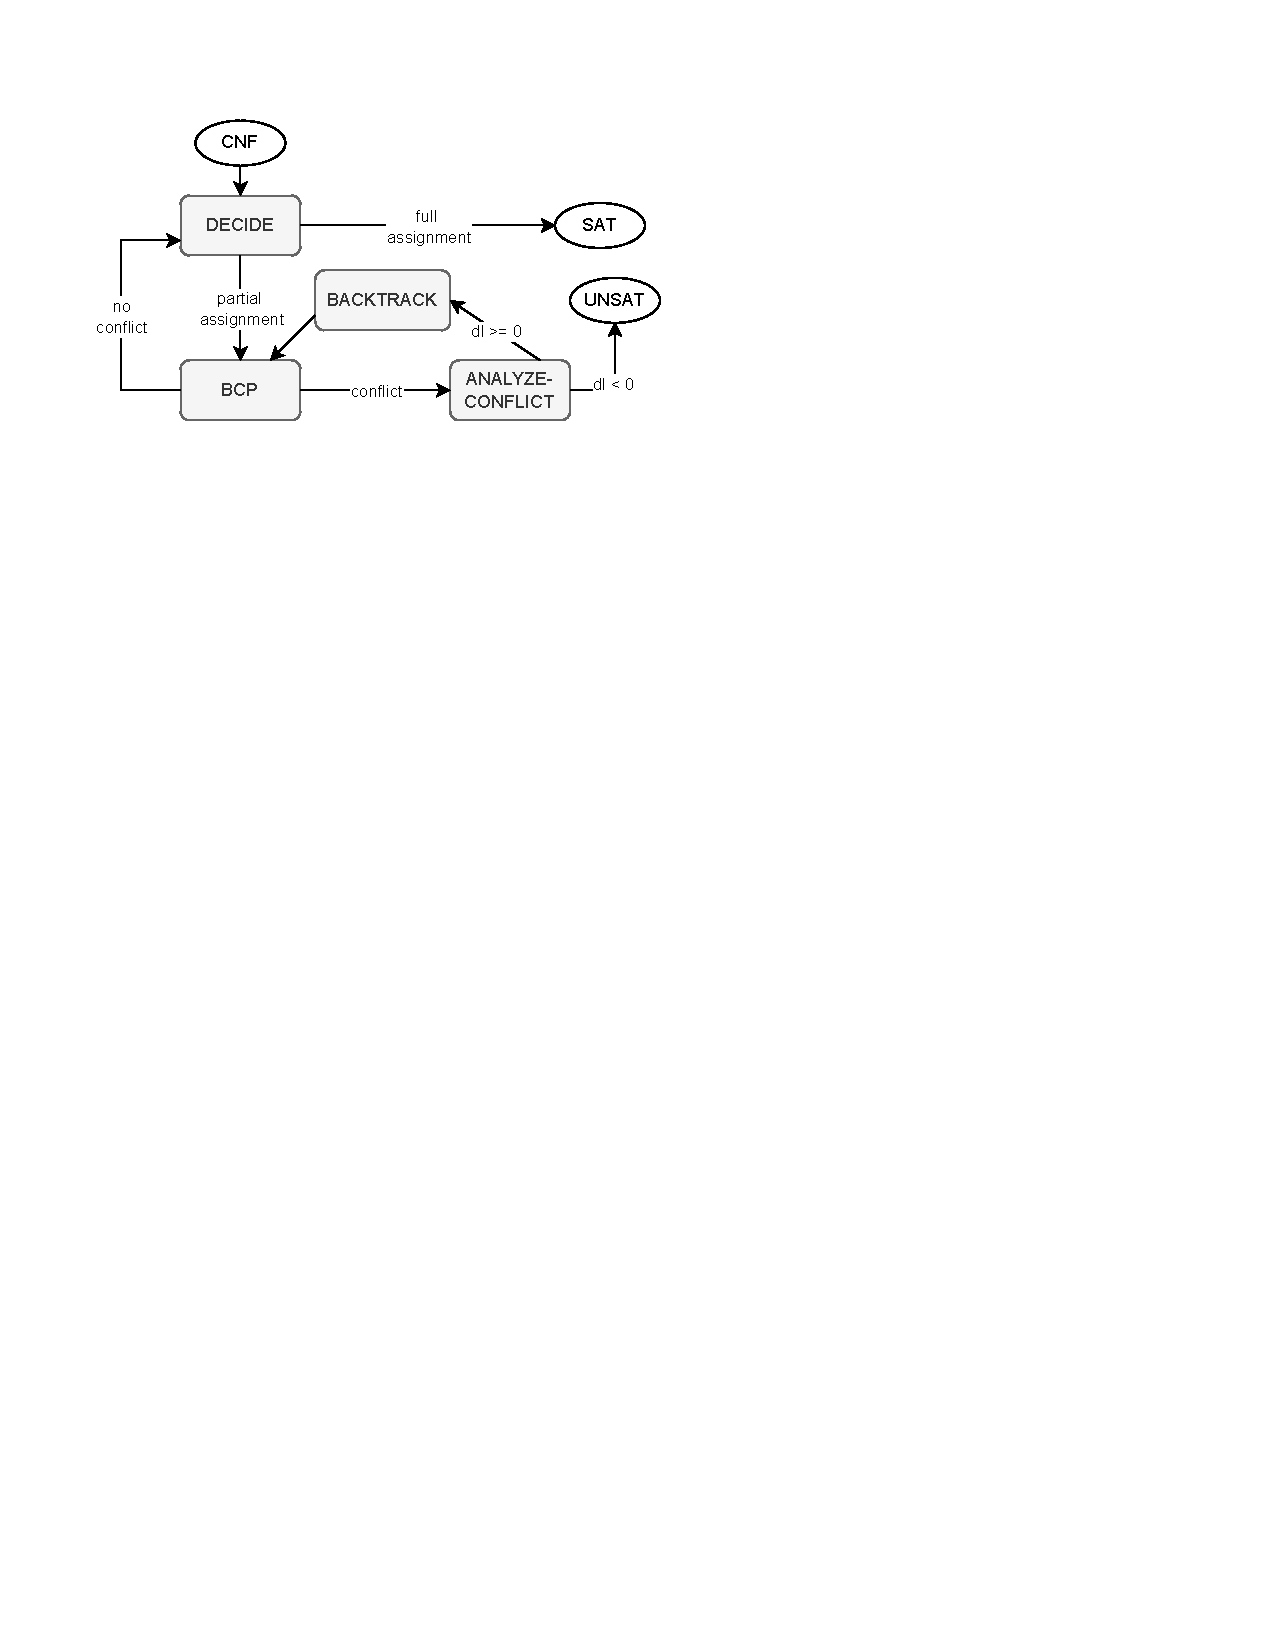
\includegraphics[width=0.8\linewidth]{figure/dpll.pdf}
  \caption{\label{fig:dpll} The classicial DPLL Algorithm.}
\end{figure}

\paragraph{DPLL} \autoref{fig:dpll} gives an overview of \textbf{DPLL}, a SAT solving technique introduced in 1961 by Davis, Putnam, Logemann, and Loveland~\cite{davis1962machine}. DPLL is an iterative algorithm that takes as input a propositional formula and (i) decides an unassigned variable and assigns it a truth value, (ii) performs Boolean constraint propagation (BCP or also called Unit Propagation),  which detects single literal clauses that either force a literal to be true in a satisfying assignment or give rise to a conflict; (iii) analyzes the conflict to backtrack to a previous decision level \texttt{dl}; and (iv) erases assignments at levels greater than \texttt{dl} to try new  assignments. These steps repeat until DPLL finds  a satisfying assignment and returns \texttt{sat}, or decides that it cannot backtrack (\texttt{dl}=-1) and returns \texttt{unsat}.


%DPLL is both sound (its results are correct) and complete (it can find a solution for any input in finite time). %Since its introduction, many heuristics have been introduced to make DPLL more efficient,
%However, because SAT solving is NP-Complete and DPLL has a worst-case exponential time complexity. %However, many heuristics have been developed to help DPLL efficient in practice,  e.g., choosing variables to assign values and decision levels to backtrack to~\cite{TODO}.


\paragraph{CDCL} Modern DPLL solving improves the original version with Conflict-Driven Clause Learning (\emph{CDCL}~\cite{bayardo1997using,marques1999grasp,569607}).
DPLL with CDCL can \emph{learn new clauses} to avoid past conflicts and backtrack more intelligently (e.g., using non-chronologically backjumping).
%Similar to DPLL, CDCL is sound and complete, but also incurs an exponential complexity.  However, 
Due to its ability to learn new clauses, CDCL can significantly  reduce the search space and allow SAT solvers to scale to large problems.
In the following, whenever we refer to DPLL, we mean DPLL with CDCL.

\paragraph{DPLL(T)} DPLL(T)~\cite{nieuwenhuis2006solving} extends DPLL for propositional formulae to check SMT formulae involving non-Boolean variables, e.g., real numbers and data structures such as strings, arrays, lists.
DPLL(T) combines DPLL with dedicated \emph{theory solvers} to analyze formulae in those theories\footnote{SMT is Satisfiability Modulo Theories and the T in DPLL(T) stands for Theories.}.  %Examples of SMT formulae include those involving numerical variables with linear or nonlinear arithmetics (formale involving nonlinear operations such as multiplication and division among variables),
For example, to check a formula involving linear arithmetic over the reals (LRA), DPLL(T) may use a theory solver that uses linear programming to check the  constraints in the formula.
Modern DPLL(T)-based SMT solvers such as Z3~\cite{moura2008z3} and CVC4~\cite{barrett2011cvc4} 
include solvers supporting a wide range of theories including linear arithmetic, nonlinear arithmetic, string, and arrays~\cite{kroening2016decision}.




\section{Linear Programming}\label{app:lp}

\tvn{Hai, give some LP background here.}

\chapter{Software vs DNN Verification}\label{app:software-vs-dnn}


\chapter{\neuralsat{} Algorithm}\label{sec:neuralsat-alg}



\SetKwInOut{Input}{input}
\SetKwInOut{Output}{output}
\SetKw{Break}{break}
\SetKw{Continue}{continue}
\SetKwFunction{Backtrack}{Backtrack}
\SetKwFunction{Decide}{Decide}
\SetKwFunction{BCP}{BCP}
\SetKwFunction{Deduction}{Deduction}
\SetKwFunction{AnalyzeConflict}{AnalyzeConflict}
\SetKwFunction{BooleanAbstraction}{BooleanAbstraction}
\SetKwFunction{AddClause}{AddClause}
\SetKwFunction{isTotal}{isTotal}
\SetKwFunction{randomattack}{RandomAttack}
\SetKwFunction{pgd}{PGDAttack}

\SetKwFunction{DPLLT}{DPLLT}
\SetKwFunction{isValid}{isValid}
\SetKwFunction{LPSolver}{LPSolver}
\SetKwFunction{Solve}{Solve}
\SetKwFunction{FindLayerNodes}{FindLayerNodes}
\SetKwFunction{TightenInputBounds}{TightenInputBounds}
\SetKwFunction{Abstract}{Abstract}
\SetKwFunction{Check}{Check}
\SetKwFunction{Decide}{Decide}
\SetKwFunction{Imply}{Imply}
\SetKwFunction{Lower}{LowerBound}
\SetKwFunction{Upper}{UpperBound}
\SetKwFunction{GetInputBounds}{GetInputBounds}
\SetKwFunction{GetInputs}{GetInputs}
\SetKwFunction{GetNumInputs}{GetNumInputs}
\SetKwFunction{CurrentConflictClause}{CurrentConflictClause}
\SetKwFunction{StopCriterion}{StopCriterion}
\SetKwFunction{LastAssignedLiteral}{LastLiteral}
\SetKwFunction{LiteralToVariable}{LiteralToVariable}
\SetKwFunction{Antecedent}{Antecedent}
\SetKwFunction{BinRes}{BinRes}
\SetKwFunction{BacktrackLevel}{BacktrackLevel}
\SetKwFunction{AddClause}{AddClause}
\SetKwFunction{ActivationStatus}{ActivationStatus}

\SetKwData{implicationgraph}{igraph}
\SetKwData{literal}{lit}
\SetKwData{variable}{var}
\SetKwData{antecedent}{ante}
\SetKwData{conflict}{conflict}
\SetKwData{none}{none}
\SetKwData{layerid}{lid}
\SetKwData{hiddenbounds}{hidden\_bounds}
\SetKwData{layerbounds}{lbounds}
\SetKwData{inputs}{inputs}
\SetKwData{inputbounds}{input\_bounds}
\SetKwData{outputbounds}{output\_bounds}
\SetKwData{infeasible}{INFEASIBLE}
\SetKwData{unreachable}{UNREACHABLE}
\SetKwData{maxinputs}{MAX\_NUM\_INPUT}
\SetKwData{assignment}{$\sigma$}
\SetKwData{network}{$\alpha$}
\SetKwData{dl}{dl}
\SetKwData{lpmodel}{solver}
\SetKwData{clauses}{clauses}
\SetKwData{conflict}{conflict}
\SetKwData{clause}{clause}
\SetKwData{igraph}{igraph}
\SetKwData{cex}{cex}

\SetKwData{true}{true}
\SetKwData{false}{false}
\DontPrintSemicolon
\SetKwFunction{Restart}{Restart}

\SetKwData{issat}{is\_sat}
\SetKwData{conflictclause}{conflict\_clause}
\SetKwData{isconflict}{is\_conflict}

\begin{algorithm}[t]
    \small
    \DontPrintSemicolon

    \Input{DNN $\alpha$, property $\phi_{in} \Rightarrow \phi_{out}$}
    \Output{\texttt{unsat} if the property is valid and \texttt{sat} otherwise}
    \BlankLine

    $\clauses \leftarrow \BooleanAbstraction(\alpha)$\;\label{line:Booleanabstraction}

    \While{\true}{
        $\sigma \leftarrow \emptyset$ \tcp{initial assignment}\label{line:varsa}
        $\dl \leftarrow 0$ \tcp{initial decision level}
        $\igraph \leftarrow \emptyset$ \tcp{initial implication graph}\label{line:varsb}
        \While{\true}{\label{line:dpllstart}
            $\isconflict \leftarrow \true$ \;

            \If{$\BCP(\clauses, \sigma, \dl, \igraph)$}{\label{line:bcp}
                \If{$\Deduction(\sigma, \dl, \alpha, \phi_{in}, \phi_{out})$}{ \label{line:deduction}
                    $\issat, v_i \leftarrow \Decide(\alpha, \phi_{in}, \phi_{out}, \dl, \sigma)$ \tcp{decision heuristic} \label{line:decide}
                    \lIf(\tcp*[h]{total assignment}){\issat}{
                        \Return{$\sat$} \label{line:returnsat}
                    }
                    $\sigma \leftarrow \sigma \land v_i$\;% \tcp{decide new variable}
                    $\dl \leftarrow \dl + 1$\;% \tcp{increase decision level by 1}
                    $\isconflict \leftarrow \false$ \tcp{mark as no conflict}
                }
            }
            \If{\isconflict}{
                \lIf(\tcp*[h]{conflict at decision level 0}){$\dl \equiv 0$}{
                    \Return{\unsat}  \label{line:unsat}
                }
                $\clause \leftarrow \AnalyzeConflict(\igraph)$\;
                $\dl \leftarrow \Backtrack(\sigma, \clause)$ \;\label{line:backtrack}
                $\clauses \leftarrow \clauses \cup \{\clause\}$ \tcp{learn conflict clauses} \label{line:learn}
            }

            \lIf(\tcp*[h]{restart heuristic}){$\Restart{}$}{\label{line:restart}
                \Break
            }
        }\label{line:dpllend}
    }
    \caption{The  \tool{}  DPLL(T) algorithm.}\label{fig:alg}

\end{algorithm}



\autoref{fig:alg} shows the \tool{} algorithm, which takes as input the formula $\alpha$ representing the ReLU-based DNN $N$ and the formulae $\phi_{in}\Rightarrow \phi_{out}$ representing the property $\phi$ to be proved.
Internally, \tool{} checks the satisfiability of the formula
\begin{equation}\label{eq:prob}
  \alpha \land \phi_{in} \land \overline{\phi_{out}}.
\end{equation}
\tool{} returns \texttt{unsat} if the formula unsatisfiable, indicating  that $\phi$ is a valid property of $N$, and \texttt{sat} if it is satisfiable, indicating the $N$ is not a valid property.

\tool{} uses a  DPLL(T)-based algorithm to check unsatisfiability.
First, the input formula in~\autoref{eq:prob} is abstracted to a propositional formula
with variables encoding neuron activation status (\texttt{BooleanAbstraction}).
Next, \tool{} assign values to Boolean variables (\texttt{Decide}) and checks for conflicts the assignment has with the real-valued constraints of the DNN and the property of interest (\texttt{BCP} and \texttt{Deduction}).
If conflicts arise, \tool{} determines the assignment decisions causing the conflicts (\texttt{AnalyzeConflict}), backtracks to erase such decisions (\texttt{Backtrack}), and learns clauses to avoid those decisions in the future.
\tool{} repeats these decisions and checking steps until it finds a total or full assignment for all Boolean variables, in which it returns \texttt{sat}, or until it no longer can backtrack and returns \texttt{unsat}.

%Note that \tool{} also resets its search (if it thinks that it is stuck in a local optima) and tries different decision orderings to enable better clause learning and avoid similar ``bad'' decisions in the previous runs.



\subsection{Boolean Abstraction}
\texttt{BooleanAbstraction} (\autoref{fig:alg}~\autoref{line:Booleanabstraction}) encodes the DNN verification problem into a Boolean constraint to be solved by DPLL.  This step creates Boolean variables to represent the \emph{activation status} of hidden neurons in the DNN. Observe that when evaluating the DNN on any concrete input, the value of each hidden neuron \emph{before} applying ReLU is either $>0$ (the neuron is \emph{active} and the input is passed through to the output) or $\le 0$ (the neuron is \emph{inactive} because the output is 0).
This allows partial assignments to these variables to represent neuron activation patterns within the DNN.

From the given network, \tool{} first creates Boolean variables representing the activation status of neurons. Next, \tool{} forms a set of initial clauses ensuring that each status variable is either \texttt{T} or \texttt{F}, indicating that each neuron is either active or inactive, respectively. A truth assignment over the variable $v_i$ creates a constraint on the pre-ReLU neuron $x_i$.


\begin{example}
For the DNN in Fig.~\ref{fig:dnn}, \tool{} creates two status variables $v_3,v_4$ for neurons $x_3,x_4$, respectively, and two initial clauses $v_3\lor \overline{v_3}$ and $v_4 \lor \overline{v_4}$. The assignment $\{x_3=T, x_4=F \}$ creates the constraint $0.5x_1-0.5x_2-1>0 \land x_1 + x_2 -2 \le 0$.
\end{example}


% neural network of verification task into set of clauses, then feed them to the solver.
% To do this, we encode each hidden node $h_i$ of the network correspond to one variable $v_i$ of the decidability problem.
% The number of variables for each hidden layer is equal to number of neurons that feed into the ReLU activation (because we want to decide the status of each ReLU node).
% In particular, in case of the linear layer, the number of hidden nodes is the hidden size $H$ of the layer itself.
% Therefore, $H$ hidden nodes are encoded as $\{v_i, v_{i+1}, ..., v_{i+H-1} \}$.
% In case of the 2-D convolution layer with input shape of $(N, C_{in}, H_{in}, W_{in})$, and output shape $(N, C_{out}, H_{out}, W_{out})$, where $N$ is the batch size, number of variables for this layer is:
% \begin{equation*}
%     H = C_{out} \times H_{out} \times W_{out}
% \end{equation*}
% After encoding all the hidden neurons into the corresponding variables, we construct a set of clauses (init\_clauses in Line 1 of Algo~\ref{fig:alg}):
% \begin{equation} \label{eq:clause}
%     (v_0 \lor \overline{v_0}) \land (v_1 \lor \overline{v_1}) \land ... \land (v_i \lor \overline{v_i}) \land (v_{i+1} \lor \overline{v_{i+1}}) \land ...
% \end{equation}
% With this form in Eq~\ref{eq:clause}, the \tool{} needs to decide all the variables to find a satisfiable solution if it exists, then returns SAT, or returns UNSAT if it could not find one.




%thus in the first step we exploit the structure of the network to create a Boolean abstraction for DPLL.

%and backtracks assignment decisions when conflicts arise.
%However, the variables in the SMT formula representing the FNN and property are real-valued, thus we exploit the structure of network to create a Boolean abstraction for DPLL.


%Thus, during preprocessing, \tool{} also creates Boolean variables representing the status values of hidden pre-ReLU neurons and an initial set of clause enforcing that each variable needs to be either $T$ (\texttt{on}) or $F$ (\texttt{off}).

\subsection{DPLL}\label{sec:dpll}

After \texttt{BooleanAbstraction}, \tool{} iteratively searches for an assignment satisfying the status clauses (Fig.~\ref{fig:alg}, lines~\ref{line:dpllstart}--~\ref{line:dpllend}).
% \tvn{something is wrong with the line ?? here} \hd{fixed}
\tool{} combines  DPLL components (e.g., \texttt{Decide}, \texttt{BCP}, \texttt{AnalyzeConflict}, \texttt{Backtrack} and \texttt{Restart}) to assign truth values with a theory solver (\S\ref{sec:deduction}), consisting of abstraction and linear programming solving, to check the feasibility of the constraints implied by the assignment with respect to the network and property of interest.

\tool{} maintains several variables (Fig.~\ref{fig:alg}, lines~\ref{line:Booleanabstraction}--~\ref{line:varsb}). These include $\clauses$, a set of \emph{clauses} consisting of the initial activation clauses and learned clauses;   $\sigma$, a \emph{truth assignment} mapping status variables to truth values; $igraph$, an \emph{implication graph} used for analyzing conflicts; and  $dl$, a non-zero \emph{decision level} used for assignment and backtracking.


%needs to analyze both \emph{Boolean constraints} (i.e., clauses involving status variables) and \emph{non-Boolean constraints} involving the nonlinear representation of the activation function and linear constraints encoding the network and status variables,  e.g., $v_3=\texttt{F}$ means $x_3'=\texttt{off}=0.5x_1-0.5x_2-1.0 \le 0$.
%To analyze both kinds of constraints,

%Fig.~\ref{fig:overview} gives an overview of \tool{}, which takes as input a DNN $N$ and a property $P$ and returns \texttt{unsat} if $P$ is a valid property of $N$ and \texttt{sat} otherwise. In the case of \texttt{sat}, \tool{} can also return a satisfying assignment representing a counterexample input violating $P$.

\subsubsection{Decide}\label{sec:decide}

From the current assignment, \texttt{Decide} (Fig.~\ref{fig:alg}, line~\ref{line:decide}) uses a heuristic to choose an unassigned variable and assigns it a random truth value at the current decision level.
\tool{} applies the Filtered Smart Branching (FSB) heuristic~\cite{bunel2018unified,de2021improved}. For each unassigned variable, FSB assumes that it has been decided (i.e., the corresponding neuron has been split) and computes a fast approximation of the lower and upperbounds of the network output variables.  FSB then prioritizes unassigned variables with the best differences among the bounds that would help make the input formula unsatisfiable (which helps prove the property of interest).
Note that if the current assignment is full, i.e., all variables have assigned values, \texttt{Decide} returns \texttt{False} (from which \tool{} returns \texttt{sat}).

% In the current implementation of \tool{}, we use two heuristics to decide unassigned variables representing activation status of neurons.
% The first is based on the bounds computed for the neurons and the second is based objective improvement approach proposed in~\cite{bunel2018unified}.



% \subsection{DPLL - CDCL}
% Modern SAT solvers employ the CDCL (Conflict-Driven Clause Learning) algorithm \cite{cdcl}, which combines the classical DPLL \cite{dpll} (Davis-Putnam-Logemann-Loveland) algorithm with clause learning.

% \textbf{DPLL} DPLL has three main components: assigning truth values to variables, inferring additional assignments from current assignments, and analyzing conflicts and backtracking to a previous decision level to try new assignments.
% Viewing the process as a search on a binary tree, each decision is associated with a decision level, which is the depth in the binary decision tree at which it is made, starting from 1.
% The assignments implied by a decision are associated with its decision level at which it occurred.

% The process of BCP is best illustrated with an implication graph.
% An implication graph represents the current partial assignment and the reason for each of the implications.
% The root nodes of an implication graph correspond to decisions, and the internal nodes to implications through BCP.
% A conflict node with incoming edges labeled with $c$ represents the fact that the BCP process has reached a conflict, by assigning 0 (False) to all the literals in the clause $c$ (i.e., $c$ is conflicting).

% \textbf{CDCL} CDCL also has these DPLL components but extends conflict analysis to learn clauses, which help avoid conflicts and backtrack more effectively.

% \textbf{DPLL(T)} DPLL(T) combines DPLL/CDCL with theory solvers to analyze formulae in different theories (e.g., using an LP solver for linear constraints).
% State-of-the-art SMT solvers such as Z3 \cite{z3} and CVC \cite{cvc} employ the DPLL(T) algorithm \cite{dpllt} to check the satisfiability of an SMT formula involving non-Boolean variables, e.g., real numbers or strings.



%\tool{} follows the DPLL(T) architecture and consists of the several main components as follows.

\subsubsection{Boolean Constraint Propagation (BCP)}\label{sec:bcp}

From the current assignment and clauses, \texttt{BCP} (Fig.~\ref{fig:alg}, line~\ref{line:bcp}) detects \emph{unit clauses}\footnote{A unit clause is a clause that has a single unassigned literal.} and infers values for variables in these clauses.
For example, after the decision $a\mapsto F$, \texttt{BCP} determines that the clause $a\vee b$ becomes unit, and infers that $b \mapsto T$.
Moreover, each assignment due to \texttt{BCP} is associated with the current decision level because instead of being ``guessed'' by \texttt{Decide} the chosen value is logically implied by other assignments.
Moreover, because each {BCP} implication might cause other clauses to become unit, \texttt{BCP} is applied repeatedly until it can no longer find unit clauses.
\textsc{BCP} returns \texttt{False} if it obtains contradictory implications (e.g., one BCP application infers $a \mapsto F$ while another infers $a \mapsto T$), and returns \texttt{True} otherwise.

\paragraph{Implication Graph} \texttt{BCP} uses an \emph{implication graph}~\cite{barrett2013decision} to represent the current assignment and the reason for each BCP implication. In this graph, a node represents the assignment and an edge $i \xrightarrow{c} j$ means that \texttt{BCP} infers the assignment represented in node $j$ due to the unit clause $c$ caused by the assignment represented by node $i$.
The implication graph is used by both BCP, which iteratively constructs the graph on each BCP application and uses it to determine conflict, and \texttt{AnalyzeConflict} (\autoref{sec:analyze-conflicts}), which analyzes the conflict in the graph to learn clauses.

\begin{figure}
    \begin{minipage}[c]{0.15\textwidth}
        \centering
        \small
        \begin{equation*}
            \begin{aligned}
                c_1 &= (\overline{v_1} \lor v_2) \\
                c_2 &= (\overline{v_1} \lor v_3 \lor v_5) \\
                c_3 &= (\overline{v_2} \lor v_4) \\
                c_4 &= (\overline{v_3} \lor \overline{v_4})
            \end{aligned}
        \end{equation*}
        \caption*{(a)}
    \end{minipage}
    \begin{minipage}[c]{0.40\textwidth}
        \centering
        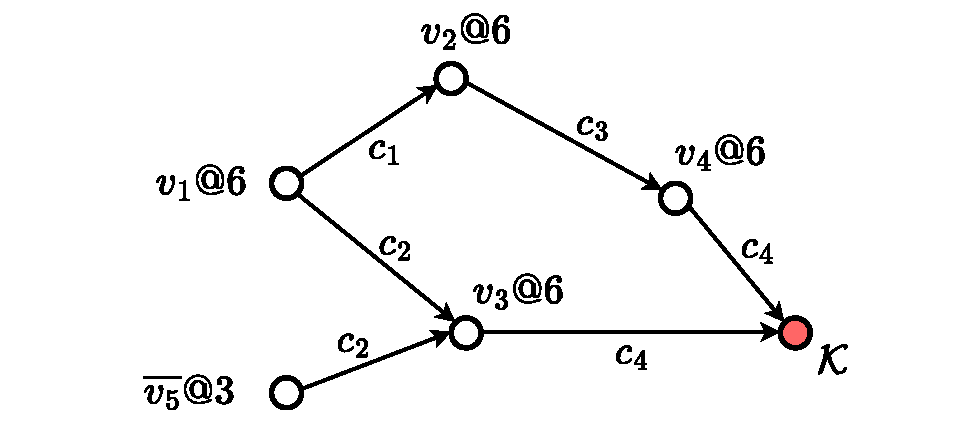
\includegraphics[width=1\linewidth]{figure/implication_graph.pdf}
        \caption*{(b)}
    \end{minipage}
    \begin{minipage}[c]{0.33\textwidth}
        \centering
        \footnotesize
        \begin{tabular}{ccccc}
            name & cl & lit & var & ante \\
            \midrule
            $c_4$ &$\overline{v_3} \lor \overline{v_4}$   & $\overline{v_3}$ &$v_3$   &     $c_2$\\
            & $\overline{v_4} \lor \overline{v_1} \lor v_5$  & $\overline{v_4}$   &     $v_4$  &      $c_3$\\
            &$\overline{v_1} \lor v_5 \lor \overline{v_2}$   & $\overline{v_2}$   &     $v_2$  &      $c_1$\\
            $c_5$      & $\overline{v_1} \lor v_5$
        \end{tabular}
        \caption*{(c)}
    \end{minipage}
    \caption{(a) A set of clauses, (b) an implication graph, and (c) learning a new clause.\label{fig:igraph}}
\end{figure}


\begin{example}
    Assume we have the clauses in Fig.~\ref{fig:igraph}(a), the assignments $\overline{v_5}@3$ and $v_1@6$ (represented in the graph in Fig.~\ref{fig:igraph}(b) by nodes  $\overline{v_5}@3$ and $v_1@6$, respectively), and are currently at decision level $dl$ 6.
Because of assignment $v_1@6$, \texttt{BCP} infers $v_2@6$ from the unit clause $c_1$ and captures that implication with edge $v_1@6 \xrightarrow{c_1} v_2@6$.
Next, because of assignment $v_2@6$, \texttt{BCP} infers $v_4@6$ from the unit clause $c_3$ as shown by edge $v_2@6 \xrightarrow{c_3} v_4@6$.

Similarly, \texttt{BCP} creates edges $v_1@6 \xrightarrow{c_2} v_3@6$ and $\overline{v_5}@ \xrightarrow{c_2} v_3@6$ to capture  the inference $v_3@6$ from the unit clause $c_2$ due to assignments $\overline{v_5}@3$ and $v_1@6$.
Now, \texttt{BCP} detects a conflict because clause $c_4=\overline{v_3} \lor \overline{v_4}$ cannot be satisfied with the assignments $v_4@6$ and $v_3@6$ (i.e., both $v_3$ and $v_4$ are $T$)  and creates two edges to the (red) node $\kappa$: $v_4@6 \xrightarrow{c_4} \kappa$ and $v_3@6 \xrightarrow{c_4} \kappa$ to capture this conflict.

Note that in this example \texttt{BCP} has the implication order $v_2,v_4,v_3$ (and then reaches a conflict). In the current implementation, \tool{} makes an arbitrary decision and thus could have a different order, e.g., $v_3, v_4,v_2$.
\end{example}

%While many SAT solvers use such arbitrary BCP implications, some use heuristics to make decisions to help reach a conflict faster~\cite{pipatsrisawat2007lightweight}.


%The implication graph is sensitive to the order in which the implications are propagated in BCP, which means that the graph is not unique for a given partial assignment. In most SAT solvers, this order is rather arbitrary (in particular, BCP progresses along a list of clauses that contain a given literal, and the order of clauses in this list can be sensitive to the order of clauses in the input CNF formula). In some other SAT solvers, this order is not arbitrary; rather, it is biased towards reaching a conflict faster. \tvn{what about in \tool{}, is the order arbitrary?}

% To illustrate the technique, we use some notations as in \cite{barrett2013decision}.
% If a variable $v_i$ is assigned 1 (owing to either a decision or an implication) at decision level \textit{dl}, we write $v_i@dl$. Similarly, $\overline{v_i}@dl$ reflects an assignment of False to this variable at decision level \textit{dl}.
% Where appropriate, we refer only to the truth assignment, omitting the decision level, in order to make the notation simpler.

% Consider, for example, a formula that contains the following set of conflict clauses, among others:
% \begin{equation}
%     \begin{aligned}
%         c_1 &= (\overline{v_1} \lor v_2) \\
%         c_2 &= (\overline{v_1} \lor v_3 \lor v_5) \\
%         c_3 &= (\overline{v_2} \lor v_4) \\
%         c_4 &= (\overline{v_3} \lor \overline{v_4}) \\
%         c_5 &= (v_1 \lor v_5 \lor \overline{v_2}) \\
%         c_6 &= (v_2 \lor v_3) \\
%         c_7 &= (v_2 \lor \overline{v_3}) \\
%         c_8 &= (v_6 \lor \overline{v_5})
%     \end{aligned}
% \end{equation}




\subsubsection{Conflict Analysis}\label{sec:analyze-conflicts}

Given an implication graph with a conflict (e.g.,~\autoref{fig:igraph}b), \texttt{AnalyzeConflict} learns a new \emph{clause} to avoid past decisions causing the conflict.
The algorithm traverses the implication graph backward, starting from the conflicting node $\kappa$, while constructing a new clause through a series of resolution steps.
\texttt{AnalyzeConflict} aims to obtain an \emph{asserting} clause, which is a clause that will force an immediate BCP implication after backtracking.


\begin{wrapfigure}{r}{0.50\textwidth}
\begin{minipage}{\linewidth}
\vspace{-0.2in}
\begin{algorithm}[H]
    \small
    \Input{implication graph \implicationgraph}
    \Output{\clause}
    \BlankLine
    $\clause \gets \CurrentConflictClause(\implicationgraph)$\;\label{line:conflict}
    \While{$\neg \StopCriterion(\clause)$}{\label{line:loopstart}
      $\literal \gets \LastAssignedLiteral(\implicationgraph, \clause)$\;\label{line:lit}
      $\variable \gets \LiteralToVariable(\literal)$\;\label{line:var}
      $\antecedent \gets \Antecedent(\implicationgraph,\literal)$\;\label{line:ante}
      $\clause \gets \BinRes(\clause, \antecedent, \variable)$\;\label{line:resolve}
    }\label{line:loopend}
    \Return{$\clause$}
    \caption{\textsc{AnalyzeConflict}}\label{alg:conflict}
  \end{algorithm}
  \end{minipage}
\end{wrapfigure}
\texttt{AnalyzeConflict}, shown in Fig.~\ref{alg:conflict}, first extracts the conflicting clause $cl$ (line~\ref{line:conflict}), represented by the edges connecting to the conflicting node $\kappa$ in the implication graph.
Next, the algorithm refines this clause to achieve an asserting clause (lines~\ref{line:loopstart}--~\ref{line:loopend}).
It obtains the literal $lit$ that was assigned last in $cl$ (line~\ref{line:lit}), the variable $var$ associated with $lit$ (line~\ref{line:var}), and the antecedent clause $ante$ of that $var$ (line~\ref{line:ante}), which contains $\overline{lit}$ as the only satisfied literal in the clause. Now, \texttt{AnalyzeConflict} resolves $cl$ and $ante$ to eliminate literals involving $var$ (line~\ref{line:resolve}). The result of the resolution is a clause, which is then refined in the next iteration.

\paragraph{Resolution.} We use the standard \emph{binary resolution rule} to learn a new clause implied by two (\emph{resolving}) clauses $a_1 \lor ... \lor a_n \lor \beta$ and $b_1 \lor ... \lor b_m \lor \overline{\beta}$ containing complementary literals involving the (\emph{resolution}) variable $\beta$:
\begin{equation} \label{eq:binary-resolution}
    \frac{(a_1 \lor ... \lor a_n \lor \beta) \quad \quad (b_1 \lor ... \lor b_m \lor \overline{\beta})}{(a_1 \lor ... \lor a_n \lor b_1 \lor ... \lor b_m)} \quad  (\textsc{Binary-Resolution})
\end{equation}
The resulting (\emph{resolvant}) clause $a_1 \lor ... \lor a_n \lor b_1 \lor ... \lor b_m$ contains all the literals that do not have complements $\beta$ and $\neg{\beta}$.
%A well-known result obtained by Robinson \cite{robinson1965machine} shows that a deductive system based on the \textbf{binary resolution} rule as its single inference rule is \textbf{sound} and \textbf{complete}.
%In other words, a CNF formula is unsatisfiable if and only if there exists a finite series of binary resolution steps ending with the empty clause.

%The function \textsc{Binary-Resolution}($c_1, c_2, v$) used in line 10 of Algorithm~\ref{alg:conflict} returns the resolvent of clauses $c_1, c_2$, where the \textbf{resolution variable} is $v$ ($\beta$ in the Equation~\ref{eq:binary-resolution}).

%\textbf{Stopping Criteria} \hd{Learned conflict clause is a special kind of conflict clause, called an \textbf{asserting} clause: it forces an immediate implication after backtracking. Empirical studies show that a good strategy for stopping criteria is to  return \textbf{true} if and only if the learned conflict clause $cl$ contains the negation of the first UIP as its single literal at the current decision level. This negated literal becomes asserted immediately after backtracking. In short, the learned conflict clause $cl$ should be an \textbf{asserting} clause.}
%(to obtain an asserting clause

% using the clauses in Fig.~\ref{fig:igraph}a and implication graph in Fig.~\ref{fig:igraph}b developed in
\begin{example}

    Fig.~\ref{fig:igraph}(c) demonstrates \texttt{AnalyzeConflict} using the example in \S\ref{sec:bcp} with the BCP implication order $v_2,v_4,v_3$ and the conflicting clause $cl$ (connecting to node $\kappa$ in the graph in Fig.~\ref{fig:igraph}(b)) $c_4=\overline{v_3} \lor \overline{v_4}$. From $c_4$, we determine the last assigned literal is $lit=\overline{v_3}$, which contains the variable $var=v_3$, and the antecedent clause containing $v_3$ is $c_2=\overline{v_1} \lor v_3 \lor v_5$ (from the implication graph in Fig.~\ref{fig:igraph}(b), we determine that assignments $v_1@6$ and $\overline{v_5}@3$ cause the BCP implication $v_3@6$ due to clause $c_2$). Now we resolve the two clauses $cl$ and $c_2$ using the resolution variable $v_3$ to obtain the clause $\overline{v_4} \lor \overline{v_1} \lor v_5$.
Next, from the new clause, we obtain $lit=\overline{v_4}, var=v_4, ante=c_3$ and apply resolution to get the clause $\overline{v_1} \vee v_5 \lor \overline{v_2}$.
Similarly, from this clause, we obtain $lit=\overline{v_2}, var=v_2, ante=c_1$ and apply resolution to obtain the clause $v_1 \lor v_5$.
% \begin{figure}
%   \centering
%   \begin{tabular}{ccccc}
%     name & cl & lit & var & ante \\
%     \midrule
%     $c_4$ &$\overline{v_3} \lor \overline{v_4}$   & $\overline{v_3}$ &$v_3$   &     $c_2$\\
%          & $\overline{v_4} \lor \overline{v_1} \lor v_5$  & $\overline{v_4}$   &     $v_4$  &      $c_3$\\
%          &$\overline{v_1} \lor v_5 \lor \overline{v_2}$   & $\overline{v_2}$   &     $v_2$  &      $c_1$\\
%     $c_5$      & $\overline{v_1} \lor v_5$

%   \end{tabular}
%   \caption{Learning a new clause.}\label{fig:igraphc}
% \end{figure}

At this point, \texttt{AnalyzeConflict} determines that this is an asserting clause, which would force an immediate BCP implication after backtracking. As will be shown in \S\ref{sec:backtrack}, \tool{} will backtrack to level 3 and erases all assignments after this level (so the assignment $\overline{v_5}@3$ is not erased, but assignments after level 3 are erased).  Then, \texttt{BCP} will find that $c_5$ is a unit clause because $\overline{v_5}@3$ and infers $\overline{v_1}$.
Once obtaining the asserting clause, \texttt{AnalyzeConflict} stops the search, and \tool{} adds  $v_1\lor v_5$ as the new clause $c_5$ to the set of existing four clauses.

\end{example}

%is a main benefit of CDCL and
The process of learning clauses allows \tool{} to learn from its past mistakes.
While such clauses are logically implied by the formula in ~\autoref{eq:prob} and therefore do not change the result, they help prune the search space and allow DPLL and therefore \tool{} to scale. For example, after learning the clause $c_5$, together with assignment $v_5@3$, we immediately infer $v_1 \mapsto F$ through BCP instead of having to guess through \texttt{Decide}.

%The literal lit is the literal in cl assigned last, and var denotes its associated variable. The antecedent clause of var, denoted by ante, contains ¬lit as the only satisfied literal, and other literals, all of which are currently unsatisfied. The clauses cl and ante thus contain lit and ¬lit, respectively, and can therefore be resolved with the resolution variable var. The resolvent clause is again a conflicting clause, which is the basis for the next resolution step.


%% After detecting the conflict, the solver determines which decision level to backtrack to according to the \textbf{conflict-driven backtracking} strategy.
%% According to this strategy, the backtracking level is set to the second most recent decision level in the conflict clause, while erasing all decisions and implications made after that level.

%% There are two special cases: when learning a \textit{unary} clause, the solver backtracks to the ground level; when the conflict is at the ground level, the backtracking level is set to –1 and the solver exits and declares the formula to be \textbf{unsatisfiable}.

%In the case of $c_9$, the solver backtracks to decision level 3 (the decision level of $v_5$), and erases all assignments from decision level 4 onwards, including the assignments to $v_1@6, v_2@6, v_3@6$, and $v_4@6$.
%The newly added conflict clause $c_9$ becomes a unit clause since $\overline{v_5}@3$, and therefore the assignment $\overline{v_1}@3$ is implied.
%This new implication restarts the BCP process at level 3.


%% Formally, the process of the analyze conflict is described in Algorithm~\ref{alg:conflict}.
%% For a given unit clause $C$ with an unassigned literal $l$, we say that $l$ is implied by $C$ and that $C$ is the \textbf{antecedent clause} of $l$, denoted by \textsc{Antecedent}($l$).
%% For example, in the example in Sec \ref{sec:bcp}, at decision level 3 the decision was $\overline{v_6}@3$, which implied $\overline{v_5}@3$ owing to clause $c_8$, hence \textsc{Antecedent}($\overline{v_5}$) = $c_8$.


%% The other functions and variables are self-explanatory.


%% The implication graph on the Fig.~\ref{fig:igraph}b demonstrates the BCP process at the current decision level 6 until, in this case, a conflict is detected.
%% The roots of this graph, namely $\overline{v_5}@3$ and $v_1@6$, constitute a sufficient condition for creating this conflict.
%% Therefore, we can safely add to our formula the \textbf{conflict clause}:
%% \begin{equation}
%%     c_9 = (v_5 \lor \overline{v_1})
%% \end{equation}


\subsubsection{Backtrack} \label{sec:backtrack}
From the clause returned by \texttt{AnalyzeConflict}, \texttt{Backtrack}  (Fig.~\ref{fig:alg}, line~\ref{line:backtrack}) computes a backtracking level and erases all decisions and implications made after that level.
If the clause is \emph{unary} (containing just a single literal), then we backtrack to level 0. % (and if we obtain further conflict with this clause, then the formula is unsatisfiable).

Currently, \tool{} uses the standard \emph{conflict-drive backtracking} strategy~\cite{barrett2013decision}, which sets the backtracking level to the \emph{second most recent} decision level in the clause.
Intuitively, by backtracking to the second most recent level, which means erasing assignments made \emph{after} that level, this strategy encourages trying new assignments for more recently decided variables.
%\hd{Other backtracking scheme in Chaff~\cite{moskewicz2001chaff}: always stop clause learning at the first UIP --- This form of clause learning, and associated backtracking procedure, is referred to as first UIP clause learning. Existing results indicate that the first UIP clause learning procedure may end up doing more backtracking than the original clause learning of GRASP~\cite{zhang2001efficient}. However, Chaff creates significantly fewer clauses and is significantly more effective at backtracking. As a result, the first UIP learning scheme is now commonly used by the majority of CDCL SAT solvers.}

%\tvn{Intuitively this is because} \hd{Intuitively, backtracking to 2nd most recent $dl$ in $cl$ to flip the assignment of the most recent decided literal (True to False or False to True). For example, \{$\neg x_5@3, x_1@6$\} causes the conflict, the most recent decided literal is $x_1$, then we need to flip $x_1$ from True to False. But now $x_1$ is associated with decision level 3 (dl 3 is decision level of $x_5$ --- the literal which has 2nd most recent decision level in the learned conflict clause.)}.



\begin{example}

    From the clause $c_5=\overline{v_1} \lor v_5$ learned in \texttt{AnalyzeConflict}, we backtrack to decision level 3, the second most recent decision level in the clause (because assignments $v_1@6$  and $\overline{v_5}@3$ were decided at levels 6 and 3, respectively). Next, we erase all assignments from decision level 4 onward (i.e., the assignments to $v_1,v_2,v_3,v_4$ as shown in the implication graph in~\autoref{fig:igraph}). This thus makes these more recently assigned variables (after decision level 3) available for new assignments (in fact, as shown by the example in~\autoref{sec:bcp}, \texttt{BCP} will immediately infer $v_1=T$ by noticing that $c_5$ is now a unit clause).
\end{example}

%\tvn{Discussion: waste of time for erasing everything from dl?} \hd{If we don't erase information from $dl$ when backtrack occurs, it will require a lot of memories to save the redundant information of implication graph from decision level $dl$ onwards.}
% \subsection{Clause Learning}
% \tvn{write pseudo code if it is complicated enough}
% \tvn{Describe }

% \tvn{Give small illustration using example in SEct 3}

% \subsection{Backtracking}
% \tvn{write pseudo code if it is complicated enough}
% \tvn{Describe }

% \tvn{Give small illustration using example in SEct 3}



%% \subsubsection{Backtrack} Given a conflict clause, \textbf{Backtrack}  (Fig.~\ref{fig:alg}, line~\ref{line:backtrack}) compute a decision level to backtrack to. Currently, we use the \emph{conflict-drive backtracking}~\cite{barrett2013decision}, which sets the backtracking level to the \emph{second most recent} decision level in the conflict clause \tvn{Intuitively this is because}.
%% Next, Backtrack erases decisions by Decide and implications by BCP and Deduce made after that level.
%% Note that if we learn a \emph{unary} clause, which contain just a single literal, then we backtrack to level 0 (and if we obtain further conflict with this clause (a conflict at level $dl=0$, line~\ref{line:unsat}), i.e., the formula is unsatisfiable).

\subsubsection{Restart}\label{sec:restart}


As with any stochastic algorithm, \tool{} can perform poorly if it gets into a subspace of the search that does not quickly lead to a solution, e.g., due to choosing a bad sequence of neurons to split~\cite{bunel2018unified,de2021improved}.
% In the development of modern SAT solver (e.g.PicoSAT~\cite{biere2008picosat}), researchers has realized most practical problems, even very large or complex, can be easily solved if they follow
This problem, which has been recognized in early SAT solving, motivates the introduction of restarting the search~\cite{gomes1998boosting} to avoid being stuck in such a \emph{local optima}.




%because the initial clause is too simple (e.g., $v_i \lor \overline{v_i}$) to make clause learning effective.

%\tvn{some more explanation on why this make clause learning ineffective}
%\hd{simple and trivial clauses lead to simple chronological backtracks by the binary resolution during conflict analysis step}
%Having said that without using restart, the non-chronological backtracks would never get used by \tool{} since these backtracks need more complex implication graph to be jumped into.

\tool{} uses a simple restart heuristic (Fig.~\ref{fig:alg}, line~\ref{line:restart}) that triggers a restart when either the number of processed assignments (nodes) exceeds a pre-defined number (e.g., 300 nodes) or the current runtime exceeds a pre-defined threshold (e.g., 50 seconds).
% \tvn{what are these number and threshold?}\hd{added}
After a restart, \tool{} avoids using the same decision order of previous runs (i.e., it would use a different sequence of neuron splittings). It also resets all internal information (e.g., decisions and implication graph) except the learned conflict clauses, which are kept and reused as these are \textit{facts} about the given constraint system.
This allows a restarted search to quickly prune parts of the  space of assignments.


%For \tool{} and DNN verification problem, we found that restart is especially important for solving difficult problem.
%Restart, which is only triggered for expensive searches, allows for a different decision ordering and assignments that might solve the problem quicker. Moreover,

We found the combination of clause learning and restarts effective for DNN verification. In particular, while restart resets information  it keeps learned clauses, which  are \emph{facts} implied by the problem, and therefore enables quicker BCP applications and non-chronological backtracking (e.g., as illustrated in Fig.~\ref{fig:tree}).

%It is worth noting that while it is possible to add a restart to existing DNN verification approaches. This is unlikely to help, because these techniques do not learn conflict clauses and therefore restart will just randomize order but carry no information forward to prune the search space.

%... \mbd{discuss possibility of restart for other tools, but it will just randomize order but carry no information forward to prune search.}

% \tvn{these are standard arguments for restart.  For \tool{} and DNN verifcation problem,  restart is even more important because the inital clause is too simple to make clause learning effective.  You should say something here about that issue.  Just write all of them here and we can clean it up}


\subsection{Deduction (Theory Solving)}\label{sec:deduction}

\begin{algorithm}[t]
    \small

    \Input{ DNN $\network$, input property $\phi_{in}$, output property $\phi_{out}$, decision level $dl$ and current assignment $\assignment$}
    \Output{{\false} if infeasibility occurs, {\true} otherwise}

    \BlankLine

    $\lpmodel \leftarrow \LPSolver(\assignment, \network \land \phi_{in} \land \overline{\phi_{out}})$\;\label{line:lpsolver}
    \lIf{$\Solve(\lpmodel) \equiv \infeasible$}{\Return {\false}}\label{line:solve}
    \lIf(\tcp*[h]{orig prob (~\autoref{eq:prob}) is satisfiable}){$\isTotal(\assignment)$}{\Return {\true} }\label{line:full}
    %$\inputs = \GetInputs(\phi_{in})$
    % $\ninputs \leftarrow \GetNumInputs(\network)$
    % $\layernodes = \FindLayerNodes(\assignment)$\;

    % \If{$|\inputs| \le \maxinputs$}{
    %     $\inputbounds = \TightenBounds(\lpmodel, \inputs)$\;\label{line:tighteninpsb}
    % }
    % \Else{$\inputbounds = \GetInputBounds(\phi_{in})$\;\label{line:inputbounds}
    % }

    $\inputbounds \leftarrow \TightenInputBounds(\lpmodel, \phi_{in})$\;\label{line:absstart}
    $\outputbounds, \hiddenbounds \leftarrow \Abstract(\network, \assignment, \inputbounds$)\;\label{line:abstraction}

    \lIf{$\Check(\outputbounds, \overline{\phi_{out}}) \equiv \infeasible$}{\Return {\false}}\label{line:checkfeasibility}

    \For{$v \in \hiddenbounds$} {\label{line:infera}
      $x \leftarrow \ActivationStatus(v)$\;
      \lIf{$x \in \sigma \lor \neg{x} \in \sigma$}{\Continue}
      \lIf{$\Lower(v) > 0$}{$\assignment \leftarrow \assignment \cup x@dl$}
        \lElseIf{$\Upper(v) \le 0$}{$\assignment \leftarrow \assignment \cup \overline{x}@dl$}\label{line:inferb}
    }

    \Return {\true}\;\label{line:absend}

    \caption{\textsc{Deduction}}\label{alg:deduction}
\end{algorithm}

\texttt{Deduction} (Fig.~\ref{fig:alg}, line~\ref{line:deduction}) is the theory or T-solver, i.e., the T in DPLL(T). The main purpose of the T-solver is to check the feasibility of the constraints represented by the current propositional variable assignment; as shown in the formalization in \S\ref{sec:formalization} this amounts to just \emph{linear equation} solving for verifying piecewise linear DNNs. However, \tool{} is able to leverage specific information from the DNN problem, including input and output properties, for more aggressive feasibility checking.  Specifically, \texttt{Deduction} has three tasks: (i) checking feasibility using linear programming (LP) solving, (i) further checking feasibility with input tightening and abstraction, and (iii) inferring literals that are unassigned and are implied by the abstracted constraint.

%The algorithm returns conflict if the current assignment does not satisfy the constraints of the network and property.
%Similar to \textsc{BCP}, Deduce also perform assignment inferencing.


Fig.~\ref{alg:deduction} describes \texttt{Deduction}, which returns \texttt{False} if infeasibility occurs and  \texttt{True} otherwise.
%\textsc{Deduce} is a theory solver that takes the arguments including: the current assignment $\sigma$, neural network $\alpha$, precondition $\phi_{in}$ over inputs and postcondition $\phi_{out}$ over outputs.
First, it creates a linear constraint system from the input assignment $\sigma$ and $\alpha \land \phi_{in} \land \overline{\phi_{out}}$, i.e., the formula in ~\autoref{eq:prob} representing the original problem  (line~\ref{line:lpsolver}).
The key idea is that we can remove ReLU activation for hidden neurons whose activation status have been decided.
For constraints in $\alpha$ associated with variables that are not in the $\sigma$,  we ignore them and just consider the cutting planes introduced by the partial assignment.
%Fixup preceding sentence based on answer.}
%\hd{Yes, you're correct. We ignore constraints generated by unassigned variables and only consider the cutting planes introduced by the partial assignment}
For example, for the assignment $v_3\mapsto T, v_4 \mapsto F$, the non-linear ReLU constraints $x_3=ReLU(-0.5x_1+0.5x_2+1)$ and  $x_4=ReLU(x_1+x_2-1)$ for the DNN in Fig.~\ref{fig:dnn} become linear constraints $x_3=-0.5x_1+0.5x_2$ and $x_4=0$, respectively.

Next, an LP solver checks the feasibility of the linear constraints (line~\ref{line:solve}).
If the solver returns infeasible,  \texttt{Deduction} returns \texttt{False} so that \tool{} can analyze the assignment and backtrack.
If the constraints are feasible, then there are two cases to handle. First, if the assignment is total (i.e., all variables are assigned), then that means that the original problem is satisfiable (line~\ref{line:full}) and \tool{} returns \texttt{sat}.

\paragraph{ReLU Abstraction.} Second, if the assignment is not total then \texttt{Deduction} applies abstraction to check satisfiability (lines~\ref{line:absstart}--\ref{line:checkfeasibility}).
Specifically, we over-approximate  ReLU computations to obtain the upper and lower bounds of the output values and check if the output properties are feasible with respect to these bounds. For example, the output $x_5 > 0$ is \emph{not} feasible if the upperbound is $x_5 \le 0$ and \emph{might be} feasible if the upperbound is $x_5 \le 0.5$ (``might be'' because this is an upper-bound). If abstraction results in infeasibility, then \texttt{Deduction} returns \texttt{False} for \tool{} to analyze the current assignment (line~\ref{line:checkfeasibility}).

\begin{figure}
    \begin{minipage}[b]{1\linewidth}
        \centering
        \begin{minipage}[c]{0.24\linewidth}
            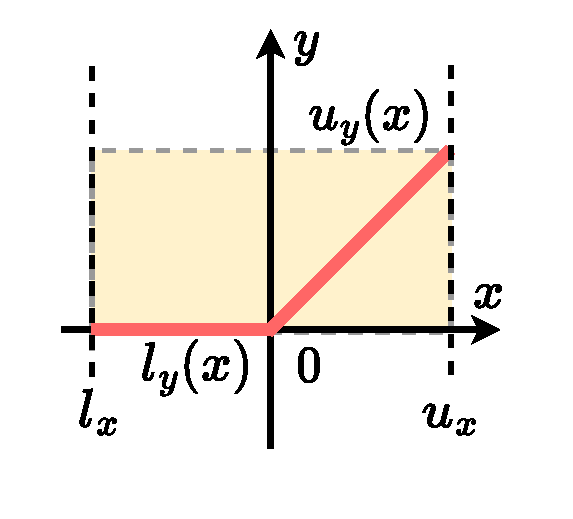
\includegraphics[width=\linewidth]{figure/interval-3.pdf}
            \vspace*{-10mm}
            \caption*{(a) interval}
        \end{minipage}
        % \hspace{0.05\textwidth}%
        \begin{minipage}[c]{0.24\linewidth}
            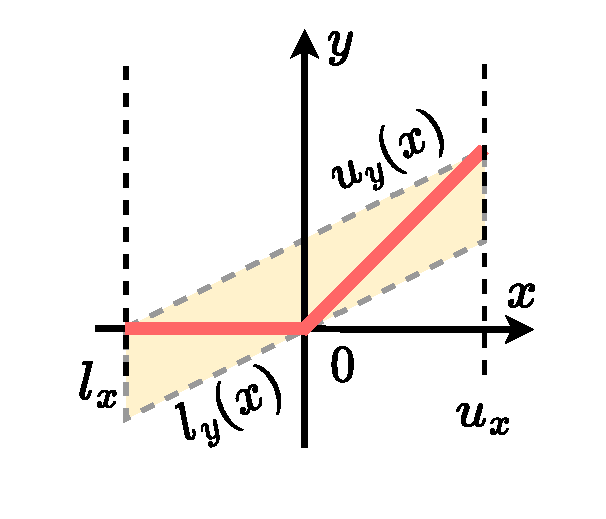
\includegraphics[width=\linewidth]{figure/zonotope-3.pdf}
            \vspace*{-10mm}
            \caption*{(b) zonotope}
        \end{minipage}
        % \hspace{0.05\textwidth}%
        \begin{minipage}[c]{0.24\linewidth}
            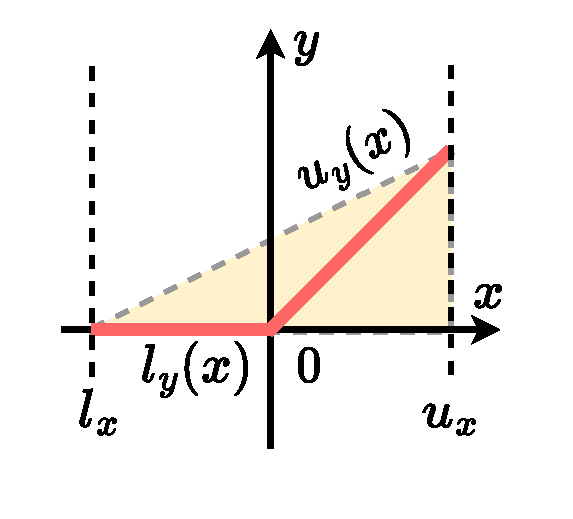
\includegraphics[width=\linewidth]{figure/polytope-3.pdf}
            \vspace*{-10mm}
            \caption*{(c) DeepPoly}
        \end{minipage}
        \begin{minipage}[c]{0.24\linewidth}
            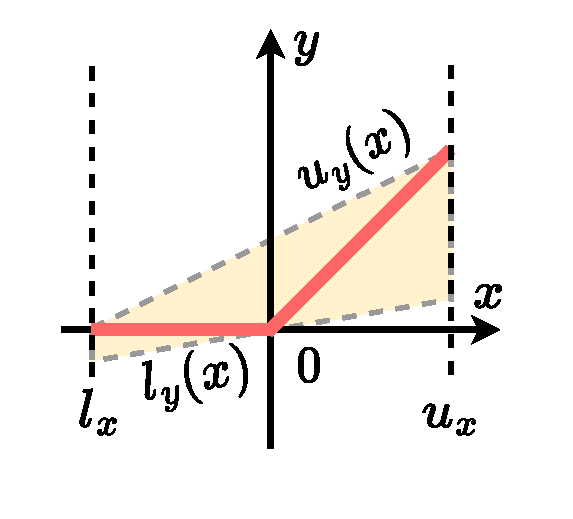
\includegraphics[width=\linewidth]{figure/lirpa-3.pdf}
            \vspace*{-10mm}
            \caption*{(d) LiRPA}
        \end{minipage}
        \vspace*{-3mm}
        \caption{Abstractions for ReLU: (a) interval, (b) zonotope, and (c-d) polytopes. Notice that ReLU is a non-convex region (red line) while all abstractions are convex regions. Note that (c) and (d) are both polytopes.}\label{fig:abs}
    \end{minipage}
\end{figure}

\tool{} uses abstraction to approximate the lower and upper bounds of hidden and output neurons.
Fig.~\ref{fig:abs} compares the (a) interval~\cite{wang2018formal}, (b) zonotope~\cite{singh2018fast}, and (c, d) polytope~\cite{xu2020fast,singh2019abstract,wang2021beta} abstraction domains to compute the lower $l_y(x)$ and upper $u_y(x)$ bounds of a ReLU computation $y=\texttt{ReLU(x)}$ (non-convex red line).
\tool{} can employ any existing abstract domains, though currently it adopts the \emph{LiRPA} polytope (Fig.~\ref{fig:abs}d)~\cite{xu2020fast,xu2020automatic,wang2021beta} because it has a good trade-off between precision and efficiency.

%Note that in some cases we can compute a better abstraction for output bounds by first tightening the input bounds (line~\ref{line:absstart}). We discuss this input bound tightening heuristic in \S\ref{sec:inputboundstigthten}.
%\hd{remove this sentence?}

\paragraph{Inference} If abstraction results in feasible constraints, \texttt{Deduction} next attempts to infer implied literals (lines~\ref{line:infera}--~\ref{line:inferb}). To obtain the bounds of the output neurons, abstraction also needs to compute the bounds of hidden neurons, including those with undecided activation status (i.e., not yet in $\sigma$).
This allows us to assign the activation variable of a hidden neuron the value
\texttt{True} if the lowerbound of that neuron is greater than 0 (the neuron is active) and
\texttt{False} otherwise.
Since each literal is considered, this would be considered exhaustive theory propagation.  Whereas the literature~\cite{nieuwenhuis2006solving,kroening2016decision} suggests that this is an inefficient strategy, we find that it does not incur significant overhead (average overhead is about 4\% and median is 2\%).

%\mbd{forward pointer to data on this in evaluation section.}
%\hd{Maximum overhead is about 39\% of runtime, all cases which have overhead > 30\% belong to CIFAR networks from CIFAR2020 benchmark which are large (cifar10\_2\_255, convBigRELU\_PGD), average overhead is about 4\%, apply median filter and average will be 2\%}

\begin{example} For the illustrative example in \autoref{ex:neuralsat}, in iteration 3, the current assignment $\sigma$ is  $\{v_4=1\}$, corresponding to a constraint $x_1 + x_2 - 1 > 0$. With the new constraint, we optimize the input bounds and compute the new bounds for hidden neurons $0.5 \le x_3 \le 2.5$, $0 < x_4 \le 2.0$ and output neuron  $x_5 \le 0.5$ (and use this to determine that the postcondition $x_5 > 0$ might be feasible). We also infer $v_3=1$ because of the positive lower bound $0.5 \le x_3$.
\end{example}

%reason
%with trade-offs between computational complexity and precision.

%\tvn{Describe how ABstractDomain works, e.g., are hidden\_bounds the bounds of values of hidden neurons? Also, how does CheckReachability work? why does it require $\phi_{in}$?}

%in which we know that the original problem is satisfiable and return (and \tool{} will return \texttt{sat}).
%The second case is when the assignment was not full, i.e., we

%% For every assignment $x\mapsto $
%% Base on the current assignment $\alpha$, first step is to build linear equations for each status variable over the input variables using back substitution.
%% The key idea here is that we could be able to remove the ReLU activation at layer $i$ if the pre-activation variables in the layer $i$ are fully assigned.
%% The ReLU function originally is non-linear (e.g., $y = max(0, x)$), but it becomes a linear function when we know about the value of its input (base on the value of assigned nodes, we could have the pre-activation values either greater or less than 0).

%% For example, the network in Figure~\ref{fig:dnn} is represented as the formula:
%% \begin{gather}
%%         x_3 = -0.5x_1 + 0.5x_2 + 1 \;\land\; x_3' = ReLU(x_3) \;\land\; \nonumber\\
%%         x_4 = x_1 + x_2 - 1 \;\land\; x_4' = ReLU(x_4)  \;\land\; \\
%%         x_5 = -x_3' + x_4' - 1 \;\nonumber
%% \end{gather}
%% If \tool{} decides $v_3 = True$ ($v_3$ is status variable of neuron $x_3'$) and $v_4$ is undecided, we cannot have the linear relationship between $x_5$ and the inputs $x_1, x_2$, because the first layer is not fully decided, then we cannot remove the ReLU layer.
%% Otherwise, \tool{} decides $v_3 = True$ and $v_4 = False$, then $x_3' = -0.5x_1 + 0.5x_2 + 1$ and $x_4' = 0$, also $x_5 = 0.5x_1 - 0.5x_2 - 2$.
%% The first layer now is fully assigned, then the ReLU layer no longer exists, that makes we could build linear relationship of $x_5$ over $x_1, x_2$.

%When all the neurons of the network are decided, the network becomes a linear one, then we could build a linear solver to check the feasibility of the model w.r.t the specification, with the constraints as linear equations of outputs over inputs.
%Branch-and-Bound based methods without the step of checking feasibility when all split neurons are also considered as \textbf{incomplete}.

%Next, these equations is added to a LP solver that follow the rule of ReLU activation: if a status variable is decided to be True, which means that neuron is in active region, its equation will be greater than 0, and constraint $eq(x) > 0$ is added to the solver; otherwise constraint $eq(x) \le 0$ is added to the solver (Line 2 in Algorithm~\ref{alg:deduction}).
%For example, $v_3 = True$ then $x_3 > 0$ and a constraint $-0.5x_1 + 0.5x_2 + 1 > 0$ is added into the LP solver.

%Then, solver runs optimization step without objective function to check the feasibility of model  (Line 3).
%If the model is infeasible, the current assignment will lead to UNSAT state, the Theory Deduce will raise ``conflict'' status so that the core DPLL could make a conflict analysis to handle it.

%Otherwise, the process continues with checking the reachability of the current assignment bases on the abstraction, described in Sec~\ref{sec:theory_abstraction}.
%Without this step, the Theory Deduce is unable to quickly decide an assignment is unreachable.
%Thus, this step uses an over-approximation technique to estimate the possible output ranges w.r.t the given input ranges and the current assignment.
%Two well-known abstraction techniques are adapted/adopted in our \tool{}, which are \textbf{DeepPoly} in ERAN verifier \cite{singh2019abstract} and \textbf{LiRPA} in $\alpha$-$\beta$-CROWN verifier\cite{wang2021beta} (Line 7).
%\hd{when does \tool{} use DeepPoly/LiRPA? Small number of inputs (<50), use LP to tighten input ranges then apply DeepPoly. Otherwise, jointly optimize hidden bounds and output bounds using LiRPA (same as ab-crown) --- Actually, in small number of inputs cases, it's reimplementation of DeepPoly with adaptation of learnable \textit{slopes} as in ab-crown. Depend on the input ranges, the abstraction will compute output ranges directly use original version or use optimized slopes version of DeepPoly to get better bounds.}
%The estimated output ranges could be used to check the reachability, as shown in Sec~\ref{sec:unsat}.
%If the output property is unreachable, the Theory Deduce will raise ``conflict'' status, otherwise, the output property might be reachable, we could not decide the reachability status of the current assignment.

\part{Optimizations and Strategies}\label{part:optimizations}

\chapter{Adversarial Attacks}\label{chap:adversarial-attacks}

Modern DNN verifiers (\crown{}, \neuralsat{}, etc) often first run an adversarial attack technique to check for obvious counterexamples. If one is found, the property is violated (and the verifier returns \sat). If no counterexample is found, the verifier proceeds to the more expensive search-based verification algorithm (e.g., \bab{} as shown in~\autoref{chap:search-algorithms}).

Thus, in the first phase of running adversarial attacks, the goal to \emph{falsify} the property, i.e., find a counterexample that violates the property. If this fails, then the goal is to \emph{verify} the property, i.e., prove that no counterexample exists. Of course, during the verification phase, the verifier may also discover counterexamples that the falsify phase misses.

\section{Random Search Attack}
Random search (RS) is a simple method for adversarial attack.  It randomly samples points in the allowed input ranges and checks if any samples violate the property; if so, a counterexample is found.

\begin{example}
Suppose the DNN input ranges are:
\[
-1 \leq x_1 \leq 1,\quad -2 \leq x_2 \leq 2
\]
and the output is:
\[
y = 2x_1 - 1.5x_2 + 1.
\]
We wish to use RS to find a counterexample to the property $y > 0$; i.e.,  trying random inputs $(x_1, x_2)$ satisfying the given ranges and producing $y \leq 0$.


\begin{itemize}
    \item Try 1: $x_1 = 0.2,\ x_2 = -0.5$
    \[
    y = 2 \times 0.2 - 1.5 \times (-0.5) + 1 = 0.4 + 0.75 + 1 = 2.15 > 0
    \]
    Not a violation.

    \item Try 2: $x_1 = -1,\ x_2 = 2$
    \[
    y = 2 \times (-1) - 1.5 \times 2 + 1 = -2 - 3 + 1 = -4 < 0
    \]
    \textbf{Counterexample found}: $(x_1 = -1,\ x_2 = 2)$.
\end{itemize}


\subsection*{2. Projected Gradient Descent (PGD)}

\textbf{Projected Gradient Descent (PGD)} is a strong first-order adversarial attack that iteratively moves the input in the direction that maximizes property violation, while projecting (clipping) the input back into the allowed domain after every step.

\begin{enumerate}
    \item \textbf{Initialize} at a valid input, e.g., $(x_1^{(0)}, x_2^{(0)}) = (0, 0)$.
    \item \textbf{For each step $t$:}
        \begin{enumerate}
            \item Compute the gradient:
            \[
            \nabla_{x} x_5 = \left( \frac{\partial x_5}{\partial x_1}, \frac{\partial x_5}{\partial x_2} \right)
            \]
            For our example,
            \[
            \nabla_{x} x_5 = (2, -1.5)
            \]
            \item Update:
            \[
            x_1^{(t+1)} = x_1^{(t)} - \eta \cdot 2
            \]
            \[
            x_2^{(t+1)} = x_2^{(t)} - \eta \cdot (-1.5)
            \]
            \item \textbf{Project (Clip)}:
            \[
            x_1^{(t+1)} = \max(-1, \min(x_1^{(t+1)}, 1))
            \]
            \[
            x_2^{(t+1)} = \max(-2, \min(x_2^{(t+1)}, 2))
            \]
            \item If $x_5 \leq 0$, \textbf{return} $(x_1^{(t+1)}, x_2^{(t+1)})$ as a counterexample.
        \end{enumerate}
\end{enumerate}

\textbf{Example:}

Let $\eta = 0.5$, initial point $(x_1, x_2) = (0, 0)$.
\begin{align*}
x_1^{(1)} &= 0 - 0.5 \times 2 = -1 \\
x_2^{(1)} &= 0 - 0.5 \times (-1.5) = 0.75 \\
\end{align*}
Clip to the ranges: $x_1^{(1)} = -1$, $x_2^{(1)} = 0.75$.

Compute:
\[
x_5 = 2 \times (-1) - 1.5 \times 0.75 + 1 = -2 - 1.125 + 1 = -2.125 < 0
\]
So, the PGD attack finds a counterexample at $(x_1 = -1,\ x_2 = 0.75)$.
% Step 2: Random Sampling
% 	•	Randomly generate x_1, x_2 values in [-2, 2].
% 	•	For example:
% 	•	Try (x_1, x_2) = (0.5, -1.0)
% 	•	x_5 = 20.5 - 1.5(-1.0) + 1 = 1 + 1.5 + 1 = 3.5 > 0 (not a violation).
% 	•	Try (x_1, x_2) = (-1, 2)
% 	•	x_5 = 2*(-1) - 1.5*2 + 1 = -2 - 3 + 1 = -4 (violation found!).

\end{example}



\chapter{Schedule}

\begin{enumerate}
    \item Week 1: 
    \item Week 2:
    \item Week 3: 
    \item Week 3:    
    \item Week 4:
    \item Week 5:
    \item Week 6:
    \item Week 7:
    \item Week 8:
    \item Week 9:
    \item Week 10:
\end{enumerate}    


\bibliographystyle{abbrv}
\bibliography{book.bib}

\appendix

\end{document}

